\documentclass{article}
\usepackage[a4paper, margin=1in]{geometry} 
\usepackage{hyperref}
\usepackage{breakurl}
\usepackage{xurl}
\usepackage{amsmath}
\usepackage{graphicx}
\usepackage{listings}
\usepackage{xcolor}
\usepackage{pgf-pie}
\usepackage{float}
\usepackage{booktabs}
\usepackage{longtable} % Per tabelle che si estendono su più pagine
\usepackage{array}     % Per allineamento avanzato delle colonne
\usepackage{tabularx}  % Per tabelle che si adattano alla larghezza della pagina
\usepackage{caption}
\usepackage{colortbl} % Per colorare le righe della tabella

% Configura la distanza tra tabella e didascalia
\captionsetup{belowskip=12pt} % Imposta uno spazio di 12pt sotto la tabella

\definecolor{darkgreen}{rgb}{0.0, 0.5, 0.0} % Verde più scuro
\definecolor{darkviolet}{rgb}{0.58, 0.0, 0.83} % Viola più intenso
\definecolor{lightred}{rgb}{1.0, 0.8, 0.8}
\definecolor{lightyellow}{rgb}{1.0, 1.0, 0.8}
\definecolor{lightgreen}{rgb}{0.8, 1.0, 0.8}


\title{Report for Domain: edison.it}
\author{Generated by Apollo}
\date{\today}

\begin{document}

\maketitle

\section*{Summary of Findings}

Below are some key statistics from the data provided:

\begin{itemize}
    \item \textbf{Number of IPs}: 134
    \item \textbf{Number of Domains}: 206
    \item \textbf{Number of Emails}: 10
    \item \textbf{Number of Resolved Hosts}: 93
    \item \textbf{Number of Mail Servers}: 4
    \item \textbf{Number of URLs}: 59
\end{itemize}

\section*{IP Addresses found}

Below is the list of IP addresses found:


\begin{itemize}
    
        \item 108.138.192.7
    
        \item 52.51.233.170
    
        \item 3.120.219.35
    
        \item 95.174.28.207
    
        \item 18.245.86.74
    
        \item 51.15.59.206
    
        \item 212.239.76.156
    
        \item 137.135.246.66
    
        \item 204.246.191.9
    
        \item 151.22.39.125
    
        \item 185.91.71.118
    
        \item 54.192.76.24
    
        \item 13.32.27.63
    
        \item 3.127.90.246
    
        \item 0.0.0.0
    
        \item 34.248.167.34
    
        \item 151.22.39.122
    
        \item 18.66.139.99
    
        \item 62.94.137.200
    
        \item 195.103.103.30
    
        \item 52.49.152.75
    
        \item 35.156.181.89
    
        \item 99.86.159.110
    
        \item 108.138.26.35
    
        \item 52.97.232.200
    
        \item 2600:9000:2490:ac00:1b:9b8a:f480:93a1
    
        \item 156.54.148.62
    
        \item 151.22.39.38
    
        \item 108.157.194.117
    
        \item 151.22.39.9
    
        \item 151.22.38.214
    
        \item 151.22.38.130
    
        \item 52.49.89.252
    
        \item 3.121.156.227
    
        \item 51.91.24.51
    
        \item 213.92.46.9
    
        \item 40.126.32.136
    
        \item 65.9.66.8
    
        \item 108.138.192.101
    
        \item 2600:9000:2490:1200:1b:9b8a:f480:93a1
    
        \item 54.192.76.109
    
        \item 151.22.38.131
    
        \item 18.195.47.200
    
        \item 18.245.46.30
    
        \item 151.22.39.19
    
        \item 151.22.39.24
    
        \item 63.33.242.246
    
        \item 37.72.32.244
    
        \item 93.186.242.241
    
        \item 3.74.25.135
    
        \item 2600:9000:2490:c200:1b:9b8a:f480:93a1
    
        \item 151.22.38.175
    
        \item 40.87.138.215
    
        \item 195.231.62.154
    
        \item 3.64.96.148
    
        \item 204.246.191.51
    
        \item 3.65.111.227
    
        \item 212.73.193.150
    
        \item 151.22.38.133
    
        \item 3.125.77.225
    
        \item 204.246.191.8
    
        \item 99.84.224.213
    
        \item 62.94.137.182
    
        \item 18.66.192.87
    
        \item 151.22.38.198
    
        \item 99.86.159.64
    
        \item 109.168.22.85
    
        \item 52.50.23.25
    
        \item 151.22.38.252
    
        \item 40.126.32.66
    
        \item 151.22.39.27
    
        \item 108.138.192.108
    
        \item 18.173.233.124
    
        \item 151.22.38.14
    
        \item 20.190.159.2
    
        \item 52.85.132.76
    
        \item 40.126.32.131
    
        \item 54.192.76.55
    
        \item 212.35.216.126
    
        \item 52.211.124.234
    
        \item 13.74.182.99
    
        \item 151.101.65.195
    
        \item 37.72.32.254
    
        \item 3.160.212.120
    
        \item 40.126.32.74
    
        \item 54.192.76.85
    
        \item 18.173.205.109
    
        \item 3.64.78.167
    
        \item 89.197.73.20
    
        \item 37.72.32.255
    
        \item 2600:9000:2729:6c00:19:89bd:7b40:93a1
    
        \item 151.22.39.163
    
        \item 3.66.39.13
    
        \item 151.22.38.13
    
        \item 93.186.249.30
    
        \item 213.217.29.85
    
        \item 3.126.218.72
    
        \item 51.75.86.118
    
        \item 151.22.38.156
    
        \item 204.246.191.61
    
        \item 51.38.105.34
    
        \item 18.202.92.68
    
        \item 151.22.39.54
    
        \item 94.124.69.67
    
        \item 151.101.1.195
    
        \item 151.22.39.18
    
        \item 162.55.172.85
    
        \item 3.160.212.90
    
        \item 151.22.38.140
    
        \item 18.66.218.109
    
        \item 20.190.160.14
    
        \item 54.76.95.70
    
        \item 83.211.69.255
    
        \item 108.156.91.85
    
        \item 37.72.32.222
    
        \item 151.22.39.6
    
        \item 3.126.233.235
    
        \item 109.168.22.86
    
        \item 46.28.2.183
    
        \item 40.126.32.6
    
        \item 151.22.38.155
    
        \item 62.94.137.206
    
        \item 151.22.39.45
    
        \item 51.178.13.239
    
        \item 108.156.2.25
    
        \item 99.86.4.85
    
        \item 94.127.86.211
    
        \item 52.213.159.238
    
        \item 62.94.137.201
    
        \item 151.22.38.152
    
        \item 151.22.38.163
    
        \item 99.84.88.78
    
        \item 151.22.38.234
    
        \item 151.22.38.70
    
\end{itemize}


\section*{Domain found}

Below is the list of Domain found:

\begin{itemize}
    
        \item crm.free.edison.it
    
        \item fmw.edison.it
    
        \item tagmanager-dnf.edison.it
    
        \item extranet2010.edison.it
    
        \item gatewaymi.edison.it
    
        \item hubatoa.edison.it
    
        \item tagmanager-140.edison.it
    
        \item qlv.free.edison.it
    
        \item tagmanager.edison.it
    
        \item portaleproduttori2.edison.it
    
        \item hub.edison.it
    
        \item MI045WLC5508CED.corp.edison.it
    
        \item ty-dev.edison.it
    
        \item lync.edison.it
    
        \item edicerpiteas01.corp.edison.it
    
        \item cbc.corp.edison.it
    
        \item password-reset.edison.it
    
        \item portalesrm.edison.it
    
        \item documentali-synergy-synvendors.edison.it
    
        \item edison.it
    
        \item niceprod.edison.it
    
        \item portale.edison.it
    
        \item er.edison.it
    
        \item mi045wlc5508ced.corp.edison.it
    
        \item ocr.edison.it
    
        \item dev-resource-edisonmysun.edison.it
    
        \item iag.free.edison.it
    
        \item EDIREPPITEAS01.corp.edison.it
    
        \item edito-test-01.corp.edison.it
    
        \item areaclienti.prep.edison.it
    
        \item stonecert.edison.it
    
        \item vpnlondon.edison.it
    
        \item enterpriseregistration.corp.edison.it
    
        \item sso.edison.it
    
        \item bonus.edison.it
    
        \item tagmanager-frendy.edison.it
    
        \item desi.corp.edison.it
    
        \item monitoraggiomar-test.edison.it
    
        \item vpn-fornitori.edison.it
    
        \item etools2.edison.it
    
        \item enterpriseregistration.egypt.edison.it
    
        \item visitatori.edison.it
    
        \item hedgingportal.corp.edison.it
    
        \item ebidtest.corp.edison.it
    
        \item cbctest.corp.edison.it
    
        \item vireoxmobile.edison.it
    
        \item facilitysolutions.edison.it
    
        \item dep.edison.it
    
        \item authsaptest.edison.it
    
        \item thorprod.corp.edison.it
    
        \item EDICERPITEAS01.corp.edison.it
    
        \item adt-temp.edison.it
    
        \item phishingalert.edison.it
    
        \item elyx.edison.it
    
        \item etools1.edison.it
    
        \item ssl-eesm-ot.edison.it
    
        \item fgt.egypt.edison.it
    
        \item edisonmediacenter.edison.it
    
        \item fgt.Egypt.edison.it
    
        \item certauth.sso.edison.it
    
        \item *.edison.it
    
        \item uag.free.edison.it
    
        \item ssl.edison.it
    
        \item ediaw01.free.edison.it
    
        \item enterpriseregistration.fenice.edison.it
    
        \item documentale-ITG.edison.it
    
        \item qvmobiletest.corp.edison.it
    
        \item portaleproduttori-qa.edison.it
    
        \item escomas-qa.edison.it
    
        \item MI045ISE3305CED.corp.edison.it
    
        \item owebapp.edison.it
    
        \item admpowerpro.edison.it
    
        \item autodiscover.edison.it
    
        \item er-fa.edison.it
    
        \item enterpriseregistration.edison.it
    
        \item collaudo-dof.edison.it
    
        \item monitoraggiomar.edison.it
    
        \item lyncdiscover.edison.it
    
        \item edisonbrandcenter.edison.it
    
        \item cbc.edison.it
    
        \item vpnclientleonardo.edison.it
    
        \item cpq-service-qa.edison.it
    
        \item eas.edison.it
    
        \item ediprdalvcms01.corp.edison.it
    
        \item energybrain-efs.edison.it
    
        \item thorprep.corp.edison.it
    
        \item free.edison.it
    
        \item sip.edison.it
    
        \item edisonnextbrandcenter.edison.it
    
        \item editstpiteas01.corp.edison.it
    
        \item ema.edison.it
    
        \item stories.efficienzaenergetica.edison.it
    
        \item srm.edison.it
    
        \item outlook.corp.edison.it
    
        \item daemobile.edison.it
    
        \item consipsl3.edison.it
    
        \item dof.edison.it
    
        \item ty.edison.it
    
        \item efficienzaenergetica.edison.it
    
        \item sancarlo.edison.it
    
        \item lead-qa.edison.it
    
        \item documentali-pandora.edison.it
    
        \item pss.edison.it
    
        \item MI045ISE3305DR.corp.edison.it
    
        \item centraleterni.edison.it
    
        \item directorsdocuments.edison.it
    
        \item adt.edison.it
    
        \item 140anni.edison.it
    
        \item vpn.edison.it
    
        \item centralesimeri.edison.it
    
        \item da.edison.it
    
        \item collaudo-noi.edison.it
    
        \item dnf.edison.it
    
        \item cmor.edison.it
    
        \item crm.prep.edison.it
    
        \item chargeandgo.edison.it
    
        \item documentale-stoccaggio.edison.it
    
        \item comparatoreofferte.edison.it
    
        \item mi045ise3305dr.corp.edison.it
    
        \item smtppub.edison.it
    
        \item gateway.edison.it
    
        \item ediema01.corp.edison.it
    
        \item epm.edison.it
    
        \item pec.edison.it
    
        \item stone.edison.it
    
        \item legacy.edison.it
    
        \item corp.edison.it
    
        \item gdc.edison.it
    
        \item edoc.edison.it
    
        \item extranet.edison.it
    
        \item enefcampus.edison.it
    
        \item noi.edison.it
    
        \item segnalazioni.edison.it
    
        \item asid.edison.it
    
        \item editoowanl01.corp.edison.it
    
        \item vpnbackup.edison.it
    
        \item wicket.edison.it
    
        \item lead-prospect-qa.edison.it
    
        \item mdm.free.edison.it
    
        \item cbcmobile.edison.it
    
        \item powerprocert.edison.it
    
        \item mies2-lotto2.edison.it
    
        \item citrix.edison.it
    
        \item webcon.edison.it
    
        \item thortestatoa.edison.it
    
        \item desitest.corp.edison.it
    
        \item commission-qa.edison.it
    
        \item iotprosumer-b2b-dev.edison.it
    
        \item elp.edison.it
    
        \item gatewayfr.edison.it
    
        \item ediema.edison.it
    
        \item er-ta.edison.it
    
        \item ediweb.edison.it
    
        \item crmee.edison.it
    
        \item wsnomitsrg.edison.it
    
        \item EDIPRDPITEAS01.corp.edison.it
    
        \item lyncws.edison.it
    
        \item softweb.edison.it
    
        \item open.edison.it
    
        \item ocr-test.edison.it
    
        \item av.edison.it
    
        \item dnf-qa.edison.it
    
        \item edireppiteas01.corp.edison.it
    
        \item gen-e.edison.it
    
        \item admpowerprocert.edison.it
    
        \item hubtest.edison.it
    
        \item stonesvil.edison.it
    
        \item cowprep.corp.edison.it
    
        \item ebid.corp.edison.it
    
        \item EDITSTPITEAS01.corp.edison.it
    
        \item teleriscaldamento.edison.it
    
        \item centraletorviscosa.edison.it
    
        \item spfk.edison.it
    
        \item trayport.edison.it
    
        \item dep2010.edison.it
    
        \item edisonfornature.edison.it
    
        \item indep2010.edison.it
    
        \item energiachecambiatutto.edison.it
    
        \item nicesvil.edison.it
    
        \item authsap.edison.it
    
        \item portaleproduttori.edison.it
    
        \item portaleproduttori1.edison.it
    
        \item ediprdpiteas01.corp.edison.it
    
        \item inge.edison.it
    
        \item wsnomitsrgtest.edison.it
    
        \item storage-hub.edison.it
    
        \item move.edison.it
    
        \item cpq-service.edison.it
    
        \item flooratrieste.edison.it
    
        \item olo2olo.edison.it
    
        \item email.edison.it
    
        \item indep.edison.it
    
        \item mi045ise3305ced.corp.edison.it
    
        \item ty-qa.edison.it
    
        \item documentale-itg.edison.it
    
        \item mi045wlc5508dr.corp.edison.it
    
        \item elearning.edison.it
    
        \item inwelldiary.edison.it
    
        \item erm.corp.edison.it
    
        \item mail.edison.it
    
        \item leonardo.edison.it
    
        \item hub.portal.edison.it
    
        \item powerpro.edison.it
    
        \item MI045WLC5508DR.corp.edison.it
    
        \item authsapdev.edison.it
    
        \item ediprdenras11.corp.edison.it
    
\end{itemize}



\section*{URLs found}

Below is the list of URLs found:

\begin{itemize}
    
        
        
        \item \href{ http://smtppub.edison.it/ }{ smtppub.edison.it }
    
        
        
        \item \href{ http://wicket.edison.it/ }{ wicket.edison.it }
    
        
        
        \item \href{ http://adt-temp.edison.it/ }{ adt-temp.edison.it }
    
        
        
        \item \href{ https://centralesimeri.edison.it/ }{ centralesimeri.edison.it }
    
        
        
        \item \href{ https://portaleproduttori-qa.edison.it/ }{ portaleproduttori-qa.edison.it }
    
        
        
        \item \href{ https://gatewaymi.edison.it/logon/LogonPoint/index.html }{ gatewaymi.edison.it }
    
        
        
        \item \href{ http://crm.free.edison.it/ }{ crm.free.edison.it }
    
        
        
        \item \href{ http://portaleproduttori.edison.it/ }{ portaleproduttori.edison.it }
    
        
        
        \item \href{ http://tagmanager-dnf.edison.it/ }{ tagmanager-dnf.edison.it }
    
        
        
        \item \href{ http://documentali-pandora.edison.it/ }{ documentali-pandora.edison.it }
    
        
        
        \item \href{ http://flooratrieste.edison.it/ }{ flooratrieste.edison.it }
    
        
        
        \item \href{ http://lead-qa.edison.it/ }{ lead-qa.edison.it }
    
        
        
        \item \href{ http://cpq-service.edison.it/ }{ cpq-service.edison.it }
    
        
        
        \item \href{ https://ty-dev.edison.it/ }{ ty-dev.edison.it }
    
        
        
        \item \href{ https://www.efficienzaenergetica.edison.it/ }{ www.efficienzaenergetica.edison.it }
    
        
        
        \item \href{ http://ediema.edison.it/ }{ ediema.edison.it }
    
        
        
        \item \href{ https://www.edison.it/en/edison-and-credit-agricole-assurances-accelerate-together-development-renewables-italy }{ www.edison.it }
    
        
        
        \item \href{ http://epm.edison.it/ }{ epm.edison.it }
    
        
        
        \item \href{ https://ty-qa.edison.it/ }{ ty-qa.edison.it }
    
        
        
        \item \href{ https://er-fa.edison.it/login/?next=/ }{ er-fa.edison.it }
    
        
        
        \item \href{ https://visitatori.edison.it/ }{ visitatori.edison.it }
    
        
        
        \item \href{ https://dnf-qa.edison.it/ }{ dnf-qa.edison.it }
    
        
        
        \item \href{ http://www.centralecandela.edison.it/ }{ www.centralecandela.edison.it }
    
        
        
        \item \href{ http://energybrain-efs.edison.it/ }{ energybrain-efs.edison.it }
    
        
        
        \item \href{ https://140anni.edison.it/ }{ 140anni.edison.it }
    
        
        
        \item \href{ https://ty.edison.it/ }{ ty.edison.it }
    
        
        
        \item \href{ http://ocr-test.edison.it/ }{ ocr-test.edison.it }
    
        
        
        \item \href{ http://tagmanager-140.edison.it/ }{ tagmanager-140.edison.it }
    
        
        
        \item \href{ http://gatewayfr.edison.it/ }{ gatewayfr.edison.it }
    
        
        
        \item \href{ http://storage-hub.edison.it/ }{ storage-hub.edison.it }
    
        
        
        \item \href{ http://vpnbackup.edison.it/ }{ vpnbackup.edison.it }
    
        
        
        \item \href{ http://tagmanager.edison.it/ }{ tagmanager.edison.it }
    
        
        
        \item \href{ http://iotprosumer-b2b-dev.edison.it/ }{ iotprosumer-b2b-dev.edison.it }
    
        
        
        \item \href{ https://portale.edison.it:52000/irj/portal }{ portale.edison.it:52000 }
    
        
        
        \item \href{ https://www.edison.it/it }{ www.edison.it }
    
        
        
        \item \href{ http://www.ediartasme.edison.it/ }{ www.ediartasme.edison.it }
    
        
        
        \item \href{ https://cpq-service-qa.edison.it/ }{ cpq-service-qa.edison.it }
    
        
        
        \item \href{ https://dnf.edison.it/ }{ dnf.edison.it }
    
        
        
        \item \href{ https://lead-prospect-qa.edison.it/ }{ lead-prospect-qa.edison.it }
    
        
        
        \item \href{ https://sancarlo.edison.it/Default.aspx }{ sancarlo.edison.it }
    
        
        
        \item \href{ https://er-fa.edison.it/saml-idp/jotx8eyawdozxjps/login/?SAMLRequest=fVLLbsIwELzzFVXueQApEIsgpdBHJBoQjx56qRxnIabEDl6Hpv36hoRWpQd8292Z2dmRh0izfU6CQqdiAYcCULduqldme4GkHvpGoQSRFDkSQTNAohlZBs9T0rEckiupJZN74x\\%2FtOosigtJcioYWTnxjFt1PZ49h9OZuPPd2EzOX9mhCXer1adLptR2IBwzAZXEfPBp3ew31BRRWOr5RyTaduZJHnoCKqq2\\%2BEYHGd5lDM3uQikF9rG9oVZy7IWIBoUBNha6EnI5rOm2z7a3aPdL1SHfw2uAmVTpcUF3vS7XOkdg2KHNDLUg4SmFxbZ\\%2BON3mS2zupywF80o9EfpW7HO293HJh\\%2F5qsY7vjIuFiez2tuAEheVqt5uZ8tlw1IsFPimMpsMhALUEdOYP1Ynrh72wOCmsr6zAsJrPaqE0ZGqNabHiqSR2FGs1ScdTdQCZlvlY8HR\\%2BCfGj\\%2FBbSa8vLnjL4B\\&RelayState=http\\%3A\\%2F\\%2Fer-edison.eu.goskope.com\\%2F\\&SigAlg=http\\%3A\\%2F\\%2Fwww.w3.org\\%2F2001\\%2F04\\%2Fxmldsig-more\\%23rsa-sha256\\&Signature=ID398c\\%2Fw2zN7vuoQ3C6TySxZaEBvNVjb\\%2BAQIJxPilU0aQ3uyGpA0jYGWrKhNSKSXhaXPaMWGOzUKyjFBQY4K4yAxb0pj\\%2FZaQQtoBf5hZhFOxz\\%2BDfmK\\%2FZCYT8NdfASlhBx0396vAHj0BLXNSsWAh3xZqG8O6NZIN3DAHopWAtzj6Vq9VK2j2LeGIRb2ZmtnDYdesnnGKfi0c62vfqcab9dO8IeYiWP2L1HRqbe2SeeRlIrD29Mkcxy99raHTCA4Cad4PTm614m18Y\\%2B6LCCX3sIc5\\%2F1eOIhrk6fQVc8bEyz\\%2Fjq1JHYHtNMPzO1bw0c\\%2Ff56usaErgcBh\\%2BDBI4MawlYZgg\\%3D\\%3D }{ er-fa.edison.it }
    
        
        
        \item \href{ https://login.microsoftonline.com/13088d93-50a5-4881-b6f2-ef681814a814/saml2?SAMLRequest=jVJha9swEP0rRt9lW3ac2CIJZAtjgXYLTdoP\\%2BzLO8rkR2JKnk8v276fYLe1gKxMciLt77909bk3Qd4Pcjf5i7vDHiOSjn31nSE6FDRudkRZIkzTQI0mv5Gl3eyOzOJWDs94q27E3kPcRQITOa2tYdNhv2HfElSorBUWeF2pRh9fmqERRLesaFEBVrVSbihaQRQ\\%2FoKCA3LBAFONGIB0MejA\\%2BpNMu5SHm2PItMLlayyL6xaB\\%2B20Qb8hLp4P5BMks4\\%2BahP3WjlLtvXWdNpgrGyfiDwty6bKeZFCwRdlKXi9bDOO7bIUpVhAiOS6Y8ai3csiH62hsUd3QvekFd7f3bxKYYfgjDaPMTaarIm1TyA4PZMkNMwfDori4TL8rZ9Fx2eTP2jThNL7\\%2FtZzE8nP5\\%2FORH7\\%2Bezmy7vorIyS\\%2B3\\%2Ff\\%2FRevTQgIfrZOvkLcd6vpkvQf2wP9pOq1\\%2FRJ\\%2Bt68P8eTsRiyuiGt1OrHA0NqHSrsWHJdlb48xC3vwE\\%3D\\&RelayState=https\\%3A\\%2F\\%2Felearning.edison.it\\%2F\\&SigAlg=http\\%3A\\%2F\\%2Fwww.w3.org\\%2F2001\\%2F04\\%2Fxmldsig-more\\%23rsa-sha256\\&Signature=ip4xo1hUfJvZwPDR6ohdEQfpRou\\%2BM3oXmsyrVnRpkXa5BG38exNCe7y\\%2BGuLBHSAYHrgUrqkLeoSIZVqdBk1\\%2Fzgpc6Wsep1RefWRvXKprHQnioafBRF78TEQ\\%2FmPmacwSTOs1mE1OhGWRszsfW\\%2F6LS\\%2F\\%2FL2m29BJCuLPPVpjVu\\%2BhJujDSN3DDivxoEzozTB4nFnvKuHfuqjrQdISPguSciZmi2pUPB\\%2FShkOdydjZm7BWvP43M9w5STrIN8E3\\%2B28OhUGmc5zyse6iH2SUnTBE11Ls7IfRzvYwG9zQKbWYQ7HHY8FxjrqQ4Z2N\\%2BtLu62DQ\\%2FWEpPTdBN26wnFT\\%2BbqoIbYyDw\\%3D\\%3D\\&sso\\_reload=true }{ login.microsoftonline.com }
    
        
        
        \item \href{ https://www.edison.it/it?utm\\_source=sendinblue\\&utm\\_campaign=NL\\_luglio\\_SENDINBLUE\\&utm\\_medium=email }{ www.edison.it }
    
        
        
        \item \href{ https://phishingalert.edison.it/ }{ phishingalert.edison.it }
    
        
        
        \item \href{ http://tagmanager-frendy.edison.it/ }{ tagmanager-frendy.edison.it }
    
        
        
        \item \href{ https://portale.edison.it:8050/sap(bD1pdCZjPTIyMCZkPW1pbg==)/bc/bsp/sap/zpqf\\_bsp\\_app/initial\\_it.htm }{ portale.edison.it:8050 }
    
        
        
        \item \href{ https://powerpro.edison.it/fe/ }{ powerpro.edison.it }
    
        
        
        \item \href{ http://commission-qa.edison.it/ }{ commission-qa.edison.it }
    
        
        
        \item \href{ https://dev-resource-edisonmysun.edison.it/ }{ dev-resource-edisonmysun.edison.it }
    
        
        
        \item \href{ http://ocr.edison.it/ }{ ocr.edison.it }
    
        
        
        \item \href{ http://srm.edison.it/ }{ srm.edison.it }
    
        
        
        \item \href{ http://gatewaymi.edison.it/ }{ gatewaymi.edison.it }
    
        
        
        \item \href{ https://escomas-qa.edison.it/ }{ escomas-qa.edison.it }
    
        
        
        \item \href{ http://centraleterni.edison.it/ }{ centraleterni.edison.it }
    
        
        
        \item \href{ https://documentali-synergy-synvendors.edison.it/account/login?ReturnUrl=\\%2Fvefa\\%2Fhome }{ documentali-synergy-synvendors.edison.it }
    
        
        
        \item \href{ http://cbcmobile.edison.it/ }{ cbcmobile.edison.it }
    
        
        
        \item \href{ http://cbc.edison.it/ }{ cbc.edison.it }
    
        
        
        \item \href{ https://er-fa.edison.it/saml-idp/jotx8eyawdozxjps/login/?SAMLRequest=fVLLbsIwELzzFVXueRFIiEWQUugDiQLi0UMvlWsvYErs4HUo7dc3JLQqPeDb7s7Mzo7cRZrtcpIWZiNnsC8ATeOmfMdsJ5FUw8QqtCSKokAiaQZIDCPz9GlEmo5Hcq2MYmpn\\%2FaNdZ1FE0EYoWdOGg8SajO9Gk4fh\\%2BLVJIxa0W4HP49hfBR7zg5hHPgvjMIhY7EUhXQXhitfUZ9BY6iRWKVt3plodBAc9Lrcm1hgMvqsc6tm90gyqYxPL6OLcHSIWMJRoqDSlkNds2V7b9joL3yNBRNrhS40blOkISU21b2NMjsR1Qdsr6gAXqKQjjHs63hY8d7fKHDvwST\\%2B4\\%2Bjpuc3R3ai2k\\%2B2uyiu1WSC7k\\%2BnpabzUIyeNiMbWnk\\%2FmiFkl\\%2FUuwriUUGeg76IBgsZ6MLf2dzUDhrVYXhMJVVRl3K0OpVYt1TTaoodG\\%2BykQcTpIof86UWm\\%2F4\\%2BzbvuX0CjLi9\\%2FTu8b\\&RelayState=http\\%3A\\%2F\\%2Fer-edison.eu.goskope.com\\%2F\\&SigAlg=http\\%3A\\%2F\\%2Fwww.w3.org\\%2F2001\\%2F04\\%2Fxmldsig-more\\%23rsa-sha256\\&Signature=eHsrVuOnDpyy8M2B1T7AqyGE5lXEGA6\\%2BYOHXoSnCNdtlc\\%2FSkLYbg\\%2FUJTSDz6jneERis5hVilZisck9xSriMo4KetMbKFeHJ36ViME\\%2FO0Nw2pnefy0VHRQdm4E9OeHzbOxsO7c6mgFjnldKAPTI4\\%2FwGGLyVgq29wzcIVxMbFeQCXfPNgRSI5dSl03Q0nSJEMB4qs7B\\%2Fc\\%2FQLYSo8qAgVBE2IZ6TSwgDhGxOlZZ7Alsg2VXAszNfCRTNPfWR\\%2BXOT8sxlCsKZw\\%2BkWc5Px9hpDRfD6LtEAUsF15vPaLUf12mVTjFp2VIS2qJjypbokc32YkEpNd0\\%2BQA68FesbhVXzXqV1KA\\%3D\\%3D }{ er-fa.edison.it }
    
        
        
        \item \href{ http://www.prep.edison.it/ }{ www.prep.edison.it }
    
\end{itemize}


\section*{Emails found}

Below is the list of Emails found:

\begin{itemize}
    
        \item edison@pec.edison.it
    
        \item ufficiostampa@edison.it
    
        \item investor.relations@edison.it
    
        \item elena.distaso@edison.it
    
        \item allacci\_subentri@edison.it
    
        \item edisonnext@pec.edison.it
    
        \item jane.doe@edison.it
    
        \item servizioclienti@edison.it
    
        \item cristina.parenti@edison.it
    
        \item '@edison.it
    
\end{itemize}

\section*{Resolved Hosts}

Below is a list of resolved hosts with their corresponding IP addresses:

\begin{itemize}
    
        \item \textbf{ 140anni.edison.it }: 108.157.194.117
    
        \item \textbf{ adt.edison.it }: 3.126.233.235
    
        \item \textbf{ authsap.edison.it }: 3.64.78.167
    
        \item \textbf{ authsapdev.edison.it }: 3.125.77.225
    
        \item \textbf{ autodiscover.edison.it }: 52.97.232.200
    
        \item \textbf{ cbc.edison.it }: 3.65.111.227
    
        \item \textbf{ cbcmobile.edison.it }: 151.22.39.24
    
        \item \textbf{ centralesimeri.edison.it }: 3.120.219.35
    
        \item \textbf{ centraleterni.edison.it }: 35.156.181.89
    
        \item \textbf{ centraletorviscosa.edison.it }: 3.126.233.235
    
        \item \textbf{ chargeandgo.edison.it }: 109.168.22.86
    
        \item \textbf{ commission-qa.edison.it }: 3.121.156.227
    
        \item \textbf{ comparatoreofferte.edison.it }: 35.156.181.89
    
        \item \textbf{ consipsl3.edison.it }: 156.54.148.62
    
        \item \textbf{ cpq-service-qa.edison.it }: 3.121.156.227
    
        \item \textbf{ cpq-service.edison.it }: 35.156.181.89
    
        \item \textbf{ crm.free.edison.it }: 151.22.38.163
    
        \item \textbf{ crm.prep.edison.it }: 151.22.38.152
    
        \item \textbf{ crmee.edison.it }: 151.22.38.156
    
        \item \textbf{ daemobile.edison.it }: 151.22.38.140
    
        \item \textbf{ dev-resource-edisonmysun.edison.it }: 108.138.192.108
    
        \item \textbf{ directorsdocuments.edison.it }: 40.87.138.215
    
        \item \textbf{ dnf-qa.edison.it }: 18.66.218.109
    
        \item \textbf{ dnf.edison.it }: 108.138.192.101
    
        \item \textbf{ documentali-pandora.edison.it }: 3.66.39.13
    
        \item \textbf{ documentali-synergy-synvendors.edison.it }: 3.65.111.227
    
        \item \textbf{ ediema.edison.it }: 151.22.38.234
    
        \item \textbf{ edison.it }: 51.75.86.118
    
        \item \textbf{ edisonbrandcenter.edison.it }: 46.28.2.183
    
        \item \textbf{ edisonfornature.edison.it }: 0.0.0.0
    
        \item \textbf{ edisonmediacenter.edison.it }: 46.28.2.183
    
        \item \textbf{ edisonnextbrandcenter.edison.it }: 46.28.2.183
    
        \item \textbf{ efficienzaenergetica.edison.it }: 54.76.95.70
    
        \item \textbf{ elearning.edison.it }: 94.124.69.67
    
        \item \textbf{ elp.edison.it }: 35.156.181.89
    
        \item \textbf{ ema.edison.it }: 3.120.219.35
    
        \item \textbf{ enefcampus.edison.it }: 51.91.24.51
    
        \item \textbf{ energybrain-efs.edison.it }: 151.22.39.125
    
        \item \textbf{ enterpriseregistration.corp.edison.it }: 40.126.32.6
    
        \item \textbf{ enterpriseregistration.edison.it }: 40.126.32.66
    
        \item \textbf{ enterpriseregistration.fenice.edison.it }: 40.126.32.131
    
        \item \textbf{ epm.edison.it }: 3.126.233.235
    
        \item \textbf{ er-fa.edison.it }: 37.72.32.255
    
        \item \textbf{ er-ta.edison.it }: 37.72.32.222
    
        \item \textbf{ er.edison.it }: 37.72.32.254
    
        \item \textbf{ escomas-qa.edison.it }: 108.156.2.25
    
        \item \textbf{ flooratrieste.edison.it }: 3.126.233.235
    
        \item \textbf{ fmw.edison.it }: 151.22.39.54
    
        \item \textbf{ gateway.edison.it }: 151.22.38.133
    
        \item \textbf{ gatewayfr.edison.it }: 3.127.90.246
    
        \item \textbf{ gatewaymi.edison.it }: 151.22.38.252
    
        \item \textbf{ gen-e.edison.it }: 93.186.242.241
    
        \item \textbf{ iag.free.edison.it }: 151.22.38.70
    
        \item \textbf{ iotprosumer-b2b-dev.edison.it }: 3.121.156.227
    
        \item \textbf{ lead-prospect-qa.edison.it }: 3.121.156.227
    
        \item \textbf{ lead-qa.edison.it }: 3.121.156.227
    
        \item \textbf{ mail.edison.it }: 151.22.38.175
    
        \item \textbf{ mies2-lotto2.edison.it }: 151.22.39.163
    
        \item \textbf{ monitoraggiomar-test.edison.it }: 63.33.242.246
    
        \item \textbf{ monitoraggiomar.edison.it }: 34.248.167.34
    
        \item \textbf{ ocr-test.edison.it }: 3.121.156.227
    
        \item \textbf{ ocr.edison.it }: 35.156.181.89
    
        \item \textbf{ olo2olo.edison.it }: 3.120.219.35
    
        \item \textbf{ open.edison.it }: 0.0.0.0
    
        \item \textbf{ phishingalert.edison.it }: 99.86.159.110
    
        \item \textbf{ portaleproduttori-qa.edison.it }: 99.86.159.64
    
        \item \textbf{ portaleproduttori.edison.it }: 3.120.219.35
    
        \item \textbf{ powerpro.edison.it }: 35.156.181.89
    
        \item \textbf{ pss.edison.it }: 151.22.38.155
    
        \item \textbf{ sancarlo.edison.it }: 151.22.39.163
    
        \item \textbf{ segnalazioni.edison.it }: 95.174.28.207
    
        \item \textbf{ smtppub.edison.it }: 151.22.38.131
    
        \item \textbf{ srm.edison.it }: 213.92.46.9
    
        \item \textbf{ ssl-eesm-ot.edison.it }: 151.22.39.122
    
        \item \textbf{ ssl.edison.it }: 151.22.38.13
    
        \item \textbf{ storage-hub.edison.it }: 3.64.96.148
    
        \item \textbf{ stories.efficienzaenergetica.edison.it }: 151.101.1.195
    
        \item \textbf{ tagmanager-140.edison.it }: 35.156.181.89
    
        \item \textbf{ tagmanager-dnf.edison.it }: 3.126.233.235
    
        \item \textbf{ tagmanager-frendy.edison.it }: 3.126.233.235
    
        \item \textbf{ tagmanager.edison.it }: 3.120.219.35
    
        \item \textbf{ ty-dev.edison.it }: 3.160.212.90
    
        \item \textbf{ ty-qa.edison.it }: 108.138.192.7
    
        \item \textbf{ ty.edison.it }: 3.160.212.120
    
        \item \textbf{ vireoxmobile.edison.it }: 37.72.32.244
    
        \item \textbf{ visitatori.edison.it }: 151.22.39.24
    
        \item \textbf{ vpn-fornitori.edison.it }: 151.22.38.133
    
        \item \textbf{ vpn.edison.it }: 151.22.38.14
    
        \item \textbf{ vpnbackup.edison.it }: 212.239.76.156
    
        \item \textbf{ vpnclientleonardo.edison.it }: 195.231.62.154
    
        \item \textbf{ wicket.edison.it }: 3.120.219.35
    
        \item \textbf{ wsnomitsrg.edison.it }: 3.74.25.135
    
        \item \textbf{ wsnomitsrgtest.edison.it }: 18.195.47.200
    
\end{itemize}

\section*{Server Mail found}

Below is the list of Server Mail found:

\begin{itemize}
    
        \item 213.217.29.85
    
        \item 185.91.71.118
    
        \item edison.esvacloud.com.
    
        \item edison2.esvacloud.com.
    
\end{itemize}

\section*{Pie Chart of Vulnerabilities}

\noindent Pie chart showing the distribution of vulnerabilities for the domain \ttfamily edison.it:

\begin{figure}[H]
    \centering
    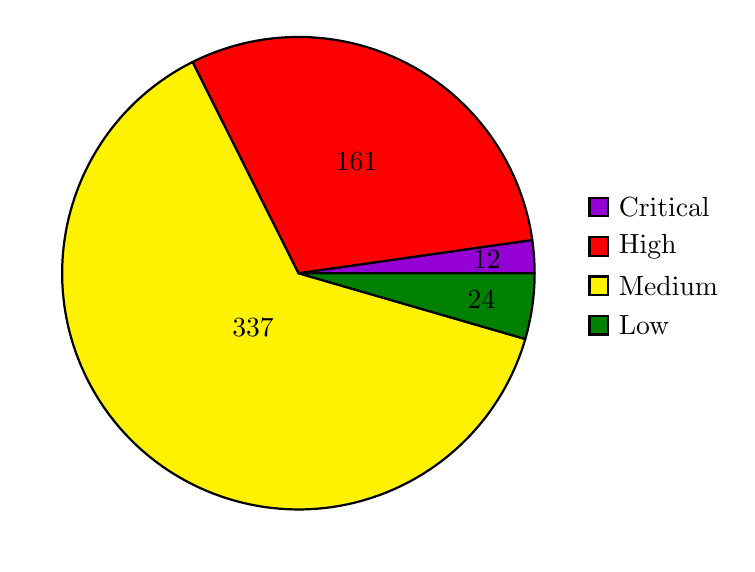
\begin{tikzpicture}
        \pie[
            color={darkviolet, red, yellow, darkgreen},
            text=legend,
            radius=3,
            sum=534
        ]
        {
            12/Critical,
            161/High,
            337/Medium,
            24/Low
        }
    \end{tikzpicture}
\end{figure}

\section*{Vulnerability Summary per IP}

\noindent The table below shows the number of critical, high, medium, and low vulnerabilities for each IP, ordered by the number of vulnerabilities (first by critical, then high, medium, and low):

\begin{longtable}{|>{\raggedright\arraybackslash}p{3cm}|c|c|c|c|}
    \hline
    \textbf{IP Address} & \textbf{Critical} & \textbf{High} & \textbf{Medium} & \textbf{Low} \\
    \hline
    \endfirsthead
    \hline
    \textbf{IP Address} & \textbf{Critical} & \textbf{High} & \textbf{Medium} & \textbf{Low} \\
    \hline
    \endhead
    \hline
    \endfoot
    \endlastfoot
    
    
    
    \rowcolor{lightred} % Righe con critical o high evidenziate in rosso
    
    156.54.148.62 & 10 & 98 & 121 & 4 \\
    \hline
    
    
    \rowcolor{lightred} % Righe con critical o high evidenziate in rosso
    
    151.22.39.163 & 2 & 4 & 20 & 2 \\
    \hline
    
    
    \rowcolor{lightred} % Righe con critical o high evidenziate in rosso
    
    109.168.22.85 & 0 & 27 & 73 & 4 \\
    \hline
    
    
    \rowcolor{lightred} % Righe con critical o high evidenziate in rosso
    
    54.76.95.70 & 0 & 26 & 106 & 10 \\
    \hline
    
    
    \rowcolor{lightred} % Righe con critical o high evidenziate in rosso
    
    212.35.216.126 & 0 & 6 & 14 & 4 \\
    \hline
    
    
    \rowcolor{lightyellow} % Righe con medium o low evidenziate in giallo
    
    109.168.22.86 & 0 & 0 & 3 & 0 \\
    \hline
    
    
    \rowcolor{lightgreen} % Righe senza vulnerabilità evidenziate in verde
    
    151.22.39.24 & 0 & 0 & 0 & 0 \\
    \hline
    
    
    \rowcolor{lightgreen} % Righe senza vulnerabilità evidenziate in verde
    
    3.65.111.227 & 0 & 0 & 0 & 0 \\
    \hline
    
    
    \rowcolor{lightgreen} % Righe senza vulnerabilità evidenziate in verde
    
    3.127.90.246 & 0 & 0 & 0 & 0 \\
    \hline
    
    
    \rowcolor{lightgreen} % Righe senza vulnerabilità evidenziate in verde
    
    62.94.137.206 & 0 & 0 & 0 & 0 \\
    \hline
    
    
    \rowcolor{lightgreen} % Righe senza vulnerabilità evidenziate in verde
    
    3.64.78.167 & 0 & 0 & 0 & 0 \\
    \hline
    
    
    \rowcolor{lightgreen} % Righe senza vulnerabilità evidenziate in verde
    
    52.49.89.252 & 0 & 0 & 0 & 0 \\
    \hline
    
    
    \rowcolor{lightgreen} % Righe senza vulnerabilità evidenziate in verde
    
    95.174.28.207 & 0 & 0 & 0 & 0 \\
    \hline
    
    
    \rowcolor{lightgreen} % Righe senza vulnerabilità evidenziate in verde
    
    151.22.38.133 & 0 & 0 & 0 & 0 \\
    \hline
    
    
    \rowcolor{lightgreen} % Righe senza vulnerabilità evidenziate in verde
    
    93.186.242.241 & 0 & 0 & 0 & 0 \\
    \hline
    
    
    \rowcolor{lightgreen} % Righe senza vulnerabilità evidenziate in verde
    
    62.94.137.182 & 0 & 0 & 0 & 0 \\
    \hline
    
    
    \rowcolor{lightgreen} % Righe senza vulnerabilità evidenziate in verde
    
    52.50.23.25 & 0 & 0 & 0 & 0 \\
    \hline
    
    
    \rowcolor{lightgreen} % Righe senza vulnerabilità evidenziate in verde
    
    151.101.65.195 & 0 & 0 & 0 & 0 \\
    \hline
    
    
    \rowcolor{lightgreen} % Righe senza vulnerabilità evidenziate in verde
    
    37.72.32.255 & 0 & 0 & 0 & 0 \\
    \hline
    
    
    \rowcolor{lightgreen} % Righe senza vulnerabilità evidenziate in verde
    
    213.217.29.85 & 0 & 0 & 0 & 0 \\
    \hline
    
    
    \rowcolor{lightgreen} % Righe senza vulnerabilità evidenziate in verde
    
    3.126.233.235 & 0 & 0 & 0 & 0 \\
    \hline
    
    
    \rowcolor{lightgreen} % Righe senza vulnerabilità evidenziate in verde
    
    3.66.39.13 & 0 & 0 & 0 & 0 \\
    \hline
    
    
    \rowcolor{lightgreen} % Righe senza vulnerabilità evidenziate in verde
    
    52.211.124.234 & 0 & 0 & 0 & 0 \\
    \hline
    
    
    \rowcolor{lightgreen} % Righe senza vulnerabilità evidenziate in verde
    
    35.156.181.89 & 0 & 0 & 0 & 0 \\
    \hline
    
    
    \rowcolor{lightgreen} % Righe senza vulnerabilità evidenziate in verde
    
    94.124.69.67 & 0 & 0 & 0 & 0 \\
    \hline
    
    
    \rowcolor{lightgreen} % Righe senza vulnerabilità evidenziate in verde
    
    151.22.39.125 & 0 & 0 & 0 & 0 \\
    \hline
    
    
    \rowcolor{lightgreen} % Righe senza vulnerabilità evidenziate in verde
    
    52.98.242.232 & 0 & 0 & 0 & 0 \\
    \hline
    
    
    \rowcolor{lightgreen} % Righe senza vulnerabilità evidenziate in verde
    
    3.121.156.227 & 0 & 0 & 0 & 0 \\
    \hline
    
    
    \rowcolor{lightgreen} % Righe senza vulnerabilità evidenziate in verde
    
    151.22.39.122 & 0 & 0 & 0 & 0 \\
    \hline
    
    
    \rowcolor{lightgreen} % Righe senza vulnerabilità evidenziate in verde
    
    151.101.1.195 & 0 & 0 & 0 & 0 \\
    \hline
    
    
    \rowcolor{lightgreen} % Righe senza vulnerabilità evidenziate in verde
    
    46.28.2.183 & 0 & 0 & 0 & 0 \\
    \hline
    
    
    \rowcolor{lightgreen} % Righe senza vulnerabilità evidenziate in verde
    
    3.120.219.35 & 0 & 0 & 0 & 0 \\
    \hline
    
    
    \rowcolor{lightgreen} % Righe senza vulnerabilità evidenziate in verde
    
    3.125.77.225 & 0 & 0 & 0 & 0 \\
    \hline
    
    
    \rowcolor{lightgreen} % Righe senza vulnerabilità evidenziate in verde
    
    51.178.13.239 & 0 & 0 & 0 & 0 \\
    \hline
    
    
    \rowcolor{lightgreen} % Righe senza vulnerabilità evidenziate in verde
    
    3.126.218.72 & 0 & 0 & 0 & 0 \\
    \hline
    
    
    \rowcolor{lightgreen} % Righe senza vulnerabilità evidenziate in verde
    
    18.202.92.68 & 0 & 0 & 0 & 0 \\
    \hline
    
    
    \rowcolor{lightgreen} % Righe senza vulnerabilità evidenziate in verde
    
    89.197.73.20 & 0 & 0 & 0 & 0 \\
    \hline
    
    
    \rowcolor{lightgreen} % Righe senza vulnerabilità evidenziate in verde
    
    3.127.119.45 & 0 & 0 & 0 & 0 \\
    \hline
    
    
    \rowcolor{lightgreen} % Righe senza vulnerabilità evidenziate in verde
    
    62.94.137.201 & 0 & 0 & 0 & 0 \\
    \hline
    
    
    \rowcolor{lightgreen} % Righe senza vulnerabilità evidenziate in verde
    
    151.22.38.13 & 0 & 0 & 0 & 0 \\
    \hline
    
    
    \rowcolor{lightgreen} % Righe senza vulnerabilità evidenziate in verde
    
    185.91.71.118 & 0 & 0 & 0 & 0 \\
    \hline
    
    
    \rowcolor{lightgreen} % Righe senza vulnerabilità evidenziate in verde
    
    52.49.152.75 & 0 & 0 & 0 & 0 \\
    \hline
    
    
    \rowcolor{lightgreen} % Righe senza vulnerabilità evidenziate in verde
    
    151.22.38.14 & 0 & 0 & 0 & 0 \\
    \hline
    
    
    \rowcolor{lightgreen} % Righe senza vulnerabilità evidenziate in verde
    
    151.22.38.252 & 0 & 0 & 0 & 0 \\
    \hline
    
    \caption{Number of vulnerabilities per IP, sorted by severity.} \\
\end{longtable}

\section*{Shodan Results for IP Addresses}

Below is the detailed report of vulnerabilities and services for each IP address:



\subsection*{IP Address: 151.22.39.24}

\begin{itemize}
    \item \textbf{Organization}: edison
    \item \textbf{Operating System}:  N/A 
    \item \textbf{Critical Vulnerabilities}: 0
    \item \textbf{High Vulnerabilities}: 0
    \item \textbf{Medium Vulnerabilities}: 0
    \item \textbf{Low Vulnerabilities}: 0
    \item \textbf{Total Vulnerabilities}: 0
\end{itemize}

\subsubsection*{Services Running on IP Address}

\begin{itemize}
    
        \item \textbf{Service}: BigIP
        \begin{itemize}
            \item \textbf{Port}: 80
            \item \textbf{Version}:  N/A 
            \item \textbf{Location}: \href{ https://151.22.39.24/ }{ https://151.22.39.24/ }
        \end{itemize}
    
        \item \textbf{Service}: N/A
        \begin{itemize}
            \item \textbf{Port}: 443
            \item \textbf{Version}:  N/A 
            \item \textbf{Location}: \href{  }{  }
        \end{itemize}
    
\end{itemize}


\textbf{No vulnerabilities found for this IP address.}




\clearpage



\subsection*{IP Address: 3.65.111.227}

\begin{itemize}
    \item \textbf{Organization}: A100 ROW GmbH
    \item \textbf{Operating System}:  N/A 
    \item \textbf{Critical Vulnerabilities}: 0
    \item \textbf{High Vulnerabilities}: 0
    \item \textbf{Medium Vulnerabilities}: 0
    \item \textbf{Low Vulnerabilities}: 0
    \item \textbf{Total Vulnerabilities}: 0
\end{itemize}

\subsubsection*{Services Running on IP Address}

\begin{itemize}
    
        \item \textbf{Service}: N/A
        \begin{itemize}
            \item \textbf{Port}: 443
            \item \textbf{Version}:  N/A 
            \item \textbf{Location}: \href{  }{  }
        \end{itemize}
    
\end{itemize}


\textbf{No vulnerabilities found for this IP address.}




\clearpage



\subsection*{IP Address: 3.127.90.246}

\begin{itemize}
    \item \textbf{Organization}: A100 ROW GmbH
    \item \textbf{Operating System}:  N/A 
    \item \textbf{Critical Vulnerabilities}: 0
    \item \textbf{High Vulnerabilities}: 0
    \item \textbf{Medium Vulnerabilities}: 0
    \item \textbf{Low Vulnerabilities}: 0
    \item \textbf{Total Vulnerabilities}: 0
\end{itemize}

\subsubsection*{Services Running on IP Address}

\begin{itemize}
    
        \item \textbf{Service}: Apache httpd
        \begin{itemize}
            \item \textbf{Port}: 443
            \item \textbf{Version}:  N/A 
            \item \textbf{Location}: \href{ / }{ / }
        \end{itemize}
    
\end{itemize}


\textbf{No vulnerabilities found for this IP address.}




\clearpage



\subsection*{IP Address: 62.94.137.206}

\begin{itemize}
    \item \textbf{Organization}: EDISON SPA
    \item \textbf{Operating System}:  N/A 
    \item \textbf{Critical Vulnerabilities}: 0
    \item \textbf{High Vulnerabilities}: 0
    \item \textbf{Medium Vulnerabilities}: 0
    \item \textbf{Low Vulnerabilities}: 0
    \item \textbf{Total Vulnerabilities}: 0
\end{itemize}

\subsubsection*{Services Running on IP Address}

\begin{itemize}
    
        \item \textbf{Service}: N/A
        \begin{itemize}
            \item \textbf{Port}: 179
            \item \textbf{Version}:  N/A 
            \item \textbf{Location}: \href{  }{  }
        \end{itemize}
    
\end{itemize}


\textbf{No vulnerabilities found for this IP address.}




\clearpage



\subsection*{IP Address: 3.64.78.167}

\begin{itemize}
    \item \textbf{Organization}: A100 ROW GmbH
    \item \textbf{Operating System}:  N/A 
    \item \textbf{Critical Vulnerabilities}: 0
    \item \textbf{High Vulnerabilities}: 0
    \item \textbf{Medium Vulnerabilities}: 0
    \item \textbf{Low Vulnerabilities}: 0
    \item \textbf{Total Vulnerabilities}: 0
\end{itemize}

\subsubsection*{Services Running on IP Address}

\begin{itemize}
    
        \item \textbf{Service}: N/A
        \begin{itemize}
            \item \textbf{Port}: 443
            \item \textbf{Version}:  N/A 
            \item \textbf{Location}: \href{ / }{ / }
        \end{itemize}
    
\end{itemize}


\textbf{No vulnerabilities found for this IP address.}




\clearpage



\subsection*{IP Address: 52.49.89.252}

\begin{itemize}
    \item \textbf{Organization}: Amazon Data Services Ireland Limited
    \item \textbf{Operating System}:  N/A 
    \item \textbf{Critical Vulnerabilities}: 0
    \item \textbf{High Vulnerabilities}: 0
    \item \textbf{Medium Vulnerabilities}: 0
    \item \textbf{Low Vulnerabilities}: 0
    \item \textbf{Total Vulnerabilities}: 0
\end{itemize}

\subsubsection*{Services Running on IP Address}

\begin{itemize}
    
        \item \textbf{Service}: AWS ELB
        \begin{itemize}
            \item \textbf{Port}: 80
            \item \textbf{Version}:  2.0 
            \item \textbf{Location}: \href{ https://52.49.89.252:443/ }{ https://52.49.89.252:443/ }
        \end{itemize}
    
        \item \textbf{Service}: AWS ELB
        \begin{itemize}
            \item \textbf{Port}: 443
            \item \textbf{Version}:  2.0 
            \item \textbf{Location}: \href{ / }{ / }
        \end{itemize}
    
\end{itemize}


\textbf{No vulnerabilities found for this IP address.}




\clearpage



\subsection*{IP Address: 95.174.28.207}

\begin{itemize}
    \item \textbf{Organization}: SEEWEB s.r.l.
    \item \textbf{Operating System}:  N/A 
    \item \textbf{Critical Vulnerabilities}: 0
    \item \textbf{High Vulnerabilities}: 0
    \item \textbf{Medium Vulnerabilities}: 0
    \item \textbf{Low Vulnerabilities}: 0
    \item \textbf{Total Vulnerabilities}: 0
\end{itemize}

\subsubsection*{Services Running on IP Address}

\begin{itemize}
    
        \item \textbf{Service}: N/A
        \begin{itemize}
            \item \textbf{Port}: 80
            \item \textbf{Version}:  N/A 
            \item \textbf{Location}: \href{ https://segnalazioni.edison.it/ }{ https://segnalazioni.edison.it/ }
        \end{itemize}
    
        \item \textbf{Service}: N/A
        \begin{itemize}
            \item \textbf{Port}: 443
            \item \textbf{Version}:  N/A 
            \item \textbf{Location}: \href{ http://wpmmuemkjmory654metcd6ibxhtmsv5t7z2ybads7kdjwrzaedfjuoqd.onion/ }{ http://wpmmuemkjmory654metcd6ibxhtmsv5t7z2ybads7kdjwrzaedfjuoqd.onion/ }
        \end{itemize}
    
\end{itemize}


\textbf{No vulnerabilities found for this IP address.}




\clearpage



\subsection*{IP Address: 151.22.38.133}

\begin{itemize}
    \item \textbf{Organization}: edison
    \item \textbf{Operating System}:  N/A 
    \item \textbf{Critical Vulnerabilities}: 0
    \item \textbf{High Vulnerabilities}: 0
    \item \textbf{Medium Vulnerabilities}: 0
    \item \textbf{Low Vulnerabilities}: 0
    \item \textbf{Total Vulnerabilities}: 0
\end{itemize}

\subsubsection*{Services Running on IP Address}

\begin{itemize}
    
        \item \textbf{Service}: N/A
        \begin{itemize}
            \item \textbf{Port}: 443
            \item \textbf{Version}:  N/A 
            \item \textbf{Location}: \href{ / }{ / }
        \end{itemize}
    
        \item \textbf{Service}: N/A
        \begin{itemize}
            \item \textbf{Port}: 10443
            \item \textbf{Version}:  N/A 
            \item \textbf{Location}: \href{ / }{ / }
        \end{itemize}
    
\end{itemize}


\textbf{No vulnerabilities found for this IP address.}




\clearpage



\subsection*{IP Address: 93.186.242.241}

\begin{itemize}
    \item \textbf{Organization}: Aruba Business srl - Dedicated Servers
    \item \textbf{Operating System}:  N/A 
    \item \textbf{Critical Vulnerabilities}: 0
    \item \textbf{High Vulnerabilities}: 0
    \item \textbf{Medium Vulnerabilities}: 0
    \item \textbf{Low Vulnerabilities}: 0
    \item \textbf{Total Vulnerabilities}: 0
\end{itemize}

\subsubsection*{Services Running on IP Address}

\begin{itemize}
    
        \item \textbf{Service}: nginx
        \begin{itemize}
            \item \textbf{Port}: 80
            \item \textbf{Version}:  N/A 
            \item \textbf{Location}: \href{ https://gen-e.edison.it/ }{ https://gen-e.edison.it/ }
        \end{itemize}
    
        \item \textbf{Service}: nginx
        \begin{itemize}
            \item \textbf{Port}: 443
            \item \textbf{Version}:  N/A 
            \item \textbf{Location}: \href{ http://www.gen-e.edison.it/ }{ http://www.gen-e.edison.it/ }
        \end{itemize}
    
\end{itemize}


\textbf{No vulnerabilities found for this IP address.}




\clearpage



\subsection*{IP Address: 62.94.137.182}

\begin{itemize}
    \item \textbf{Organization}: EDF EN Service Italia
    \item \textbf{Operating System}:  N/A 
    \item \textbf{Critical Vulnerabilities}: 0
    \item \textbf{High Vulnerabilities}: 0
    \item \textbf{Medium Vulnerabilities}: 0
    \item \textbf{Low Vulnerabilities}: 0
    \item \textbf{Total Vulnerabilities}: 0
\end{itemize}

\subsubsection*{Services Running on IP Address}

\begin{itemize}
    
        \item \textbf{Service}: N/A
        \begin{itemize}
            \item \textbf{Port}: 179
            \item \textbf{Version}:  N/A 
            \item \textbf{Location}: \href{  }{  }
        \end{itemize}
    
\end{itemize}


\textbf{No vulnerabilities found for this IP address.}




\clearpage



\subsection*{IP Address: 52.50.23.25}

\begin{itemize}
    \item \textbf{Organization}: Amazon Data Services Ireland Limited
    \item \textbf{Operating System}:  N/A 
    \item \textbf{Critical Vulnerabilities}: 0
    \item \textbf{High Vulnerabilities}: 0
    \item \textbf{Medium Vulnerabilities}: 0
    \item \textbf{Low Vulnerabilities}: 0
    \item \textbf{Total Vulnerabilities}: 0
\end{itemize}

\subsubsection*{Services Running on IP Address}

\begin{itemize}
    
        \item \textbf{Service}: N/A
        \begin{itemize}
            \item \textbf{Port}: 443
            \item \textbf{Version}:  N/A 
            \item \textbf{Location}: \href{ / }{ / }
        \end{itemize}
    
\end{itemize}


\textbf{No vulnerabilities found for this IP address.}




\clearpage



\subsection*{IP Address: 151.101.65.195}

\begin{itemize}
    \item \textbf{Organization}: Fastly, Inc.
    \item \textbf{Operating System}:  N/A 
    \item \textbf{Critical Vulnerabilities}: 0
    \item \textbf{High Vulnerabilities}: 0
    \item \textbf{Medium Vulnerabilities}: 0
    \item \textbf{Low Vulnerabilities}: 0
    \item \textbf{Total Vulnerabilities}: 0
\end{itemize}

\subsubsection*{Services Running on IP Address}

\begin{itemize}
    
        \item \textbf{Service}: N/A
        \begin{itemize}
            \item \textbf{Port}: 80
            \item \textbf{Version}:  N/A 
            \item \textbf{Location}: \href{ https://haveyouseenthis.dog/ }{ https://haveyouseenthis.dog/ }
        \end{itemize}
    
        \item \textbf{Service}: N/A
        \begin{itemize}
            \item \textbf{Port}: 443
            \item \textbf{Version}:  N/A 
            \item \textbf{Location}: \href{ / }{ / }
        \end{itemize}
    
\end{itemize}


\textbf{No vulnerabilities found for this IP address.}




\clearpage



\subsection*{IP Address: 37.72.32.255}

\begin{itemize}
    \item \textbf{Organization}: Netalia DTC Milano
    \item \textbf{Operating System}:  N/A 
    \item \textbf{Critical Vulnerabilities}: 0
    \item \textbf{High Vulnerabilities}: 0
    \item \textbf{Medium Vulnerabilities}: 0
    \item \textbf{Low Vulnerabilities}: 0
    \item \textbf{Total Vulnerabilities}: 0
\end{itemize}

\subsubsection*{Services Running on IP Address}

\begin{itemize}
    
        \item \textbf{Service}: N/A
        \begin{itemize}
            \item \textbf{Port}: 179
            \item \textbf{Version}:  N/A 
            \item \textbf{Location}: \href{  }{  }
        \end{itemize}
    
\end{itemize}


\textbf{No vulnerabilities found for this IP address.}




\clearpage



\subsection*{IP Address: 213.217.29.85}

\begin{itemize}
    \item \textbf{Organization}: Libraesva srl
    \item \textbf{Operating System}:  N/A 
    \item \textbf{Critical Vulnerabilities}: 0
    \item \textbf{High Vulnerabilities}: 0
    \item \textbf{Medium Vulnerabilities}: 0
    \item \textbf{Low Vulnerabilities}: 0
    \item \textbf{Total Vulnerabilities}: 0
\end{itemize}

\subsubsection*{Services Running on IP Address}

\begin{itemize}
    
        \item \textbf{Service}: Postfix smtpd
        \begin{itemize}
            \item \textbf{Port}: 25
            \item \textbf{Version}:  N/A 
            \item \textbf{Location}: \href{  }{  }
        \end{itemize}
    
        \item \textbf{Service}: Apache httpd
        \begin{itemize}
            \item \textbf{Port}: 80
            \item \textbf{Version}:  N/A 
            \item \textbf{Location}: \href{ https://213.217.29.85/ }{ https://213.217.29.85/ }
        \end{itemize}
    
        \item \textbf{Service}: Postfix smtpd
        \begin{itemize}
            \item \textbf{Port}: 465
            \item \textbf{Version}:  N/A 
            \item \textbf{Location}: \href{  }{  }
        \end{itemize}
    
        \item \textbf{Service}: Postfix smtpd
        \begin{itemize}
            \item \textbf{Port}: 587
            \item \textbf{Version}:  N/A 
            \item \textbf{Location}: \href{  }{  }
        \end{itemize}
    
\end{itemize}


\textbf{No vulnerabilities found for this IP address.}




\clearpage



\subsection*{IP Address: 3.126.233.235}

\begin{itemize}
    \item \textbf{Organization}: A100 ROW GmbH
    \item \textbf{Operating System}:  N/A 
    \item \textbf{Critical Vulnerabilities}: 0
    \item \textbf{High Vulnerabilities}: 0
    \item \textbf{Medium Vulnerabilities}: 0
    \item \textbf{Low Vulnerabilities}: 0
    \item \textbf{Total Vulnerabilities}: 0
\end{itemize}

\subsubsection*{Services Running on IP Address}

\begin{itemize}
    
        \item \textbf{Service}: N/A
        \begin{itemize}
            \item \textbf{Port}: 443
            \item \textbf{Version}:  N/A 
            \item \textbf{Location}: \href{  }{  }
        \end{itemize}
    
\end{itemize}


\textbf{No vulnerabilities found for this IP address.}




\clearpage



\subsection*{IP Address: 212.35.216.126}

\begin{itemize}
    \item \textbf{Organization}: SEEWEB s.r.l.
    \item \textbf{Operating System}:  N/A 
    \item \textbf{Critical Vulnerabilities}: 0
    \item \textbf{High Vulnerabilities}: 6
    \item \textbf{Medium Vulnerabilities}: 14
    \item \textbf{Low Vulnerabilities}: 4
    \item \textbf{Total Vulnerabilities}: 24
\end{itemize}

\subsubsection*{Services Running on IP Address}

\begin{itemize}
    
        \item \textbf{Service}: Apache httpd
        \begin{itemize}
            \item \textbf{Port}: 80
            \item \textbf{Version}:  2.4.57 
            \item \textbf{Location}: \href{ / }{ / }
        \end{itemize}
    
\end{itemize}


\subsubsection*{Vulnerabilities Found}

\begin{itemize}
    
        \item \textbf{Vulnerability}: CVE-2013-0941
        \begin{itemize}
            \item \textbf{CVSS Score}:  2.1 
            \item \textbf{Description}:
            \parbox[t]{0.9\linewidth}{
                \ttfamily EMC RSA Authentication API before 8.1 SP1, RSA Web Agent before 5.3.5 for Apache Web Server, RSA Web Agent before 5.3.5 for IIS, RSA PAM Agent before 7.0, and RSA Agent before 6.1.4 for Microsoft Windows use an improper encryption algorithm and a weak key for maintaining the stored data of the node secret for the SecurID Authentication API, which allows local users to obtain sensitive information via cryptographic attacks on this data.
            }
        \end{itemize}
    
        \item \textbf{Vulnerability}: CVE-2013-0942
        \begin{itemize}
            \item \textbf{CVSS Score}:  4.3 
            \item \textbf{Description}:
            \parbox[t]{0.9\linewidth}{
                \ttfamily Cross-site scripting (XSS) vulnerability in EMC RSA Authentication Agent 7.1 before 7.1.1 for Web for Internet Information Services, and 7.1 before 7.1.1 for Web for Apache, allows remote attackers to inject arbitrary web script or HTML via unspecified vectors.
            }
        \end{itemize}
    
        \item \textbf{Vulnerability}: CVE-2012-4001
        \begin{itemize}
            \item \textbf{CVSS Score}:  5 
            \item \textbf{Description}:
            \parbox[t]{0.9\linewidth}{
                \ttfamily The mod\_pagespeed module before 0.10.22.6 for the Apache HTTP Server does not properly verify its host name, which allows remote attackers to trigger HTTP requests to arbitrary hosts via unspecified vectors, as demonstrated by requests to intranet servers.
            }
        \end{itemize}
    
        \item \textbf{Vulnerability}: CVE-2009-2299
        \begin{itemize}
            \item \textbf{CVSS Score}:  5 
            \item \textbf{Description}:
            \parbox[t]{0.9\linewidth}{
                \ttfamily The Artofdefence Hyperguard Web Application Firewall (WAF) module before 2.5.5-11635, 3.0 before 3.0.3-11636, and 3.1 before 3.1.1-11637, a module for the Apache HTTP Server, allows remote attackers to cause a denial of service (memory consumption) via an HTTP request with a large Content-Length value but no POST data.
            }
        \end{itemize}
    
        \item \textbf{Vulnerability}: CVE-2024-27316
        \begin{itemize}
            \item \textbf{CVSS Score}:  N/A 
            \item \textbf{Description}:
            \parbox[t]{0.9\linewidth}{
                \ttfamily HTTP/2 incoming headers exceeding the limit are temporarily buffered in nghttp2 in order to generate an informative HTTP 413 response. If a client does not stop sending headers, this leads to memory exhaustion.
            }
        \end{itemize}
    
        \item \textbf{Vulnerability}: CVE-2023-31122
        \begin{itemize}
            \item \textbf{CVSS Score}:  N/A 
            \item \textbf{Description}:
            \parbox[t]{0.9\linewidth}{
                \ttfamily Out-of-bounds Read vulnerability in mod\_macro of Apache HTTP Server.This issue affects Apache HTTP Server: through 2.4.57.
            }
        \end{itemize}
    
        \item \textbf{Vulnerability}: CVE-2013-2765
        \begin{itemize}
            \item \textbf{CVSS Score}:  5 
            \item \textbf{Description}:
            \parbox[t]{0.9\linewidth}{
                \ttfamily The ModSecurity module before 2.7.4 for the Apache HTTP Server allows remote attackers to cause a denial of service (NULL pointer dereference, process crash, and disk consumption) via a POST request with a large body and a crafted Content-Type header.
            }
        \end{itemize}
    
        \item \textbf{Vulnerability}: CVE-2011-1176
        \begin{itemize}
            \item \textbf{CVSS Score}:  4.3 
            \item \textbf{Description}:
            \parbox[t]{0.9\linewidth}{
                \ttfamily The configuration merger in itk.c in the Steinar H. Gunderson mpm-itk Multi-Processing Module 2.2.11-01 and 2.2.11-02 for the Apache HTTP Server does not properly handle certain configuration sections that specify NiceValue but not AssignUserID, which might allow remote attackers to gain privileges by leveraging the root uid and root gid of an mpm-itk process.
            }
        \end{itemize}
    
        \item \textbf{Vulnerability}: CVE-2023-45802
        \begin{itemize}
            \item \textbf{CVSS Score}:  N/A 
            \item \textbf{Description}:
            \parbox[t]{0.9\linewidth}{
                \ttfamily When a HTTP/2 stream was reset (RST frame) by a client, there was a time window were the request's memory resources were not reclaimed immediately. Instead, de-allocation was deferred to connection close. A client could send new requests and resets, keeping the connection busy and open and causing the memory footprint to keep on growing. On connection close, all resources were reclaimed, but the process might run out of memory before that.This was found by the reporter during testing ofCVE-2023-44487 (HTTP/2 Rapid Reset Exploit) with their own test client. During "normal" HTTP/2 use, the probability to hit this bug is very low. The kept memory would not become noticeable before the connection closes or times out.Users are recommended to upgrade to version 2.4.58, which fixes the issue.
            }
        \end{itemize}
    
        \item \textbf{Vulnerability}: CVE-2011-2688
        \begin{itemize}
            \item \textbf{CVSS Score}:  7.5 
            \item \textbf{Description}:
            \parbox[t]{0.9\linewidth}{
                \ttfamily SQL injection vulnerability in mysql/mysql-auth.pl in the mod\_authnz\_external module 3.2.5 and earlier for the Apache HTTP Server allows remote attackers to execute arbitrary SQL commands via the user field.
            }
        \end{itemize}
    
        \item \textbf{Vulnerability}: CVE-2009-0796
        \begin{itemize}
            \item \textbf{CVSS Score}:  2.6 
            \item \textbf{Description}:
            \parbox[t]{0.9\linewidth}{
                \ttfamily Cross-site scripting (XSS) vulnerability in Status.pm in Apache::Status and Apache2::Status in mod\_perl1 and mod\_perl2 for the Apache HTTP Server, when /perl-status is accessible, allows remote attackers to inject arbitrary web script or HTML via the URI.
            }
        \end{itemize}
    
        \item \textbf{Vulnerability}: CVE-2023-43622
        \begin{itemize}
            \item \textbf{CVSS Score}:  N/A 
            \item \textbf{Description}:
            \parbox[t]{0.9\linewidth}{
                \ttfamily An attacker, opening a HTTP/2 connection with an initial window size of 0, was able to block handling of that connection indefinitely in Apache HTTP Server. This could be used to exhaust worker resources in the server, similar to the well known "slow loris" attack pattern.This has been fixed in version 2.4.58, so that such connection are terminated properly after the configured connection timeout.This issue affects Apache HTTP Server: from 2.4.55 through 2.4.57.Users are recommended to upgrade to version 2.4.58, which fixes the issue.
            }
        \end{itemize}
    
        \item \textbf{Vulnerability}: CVE-2007-4723
        \begin{itemize}
            \item \textbf{CVSS Score}:  7.5 
            \item \textbf{Description}:
            \parbox[t]{0.9\linewidth}{
                \ttfamily Directory traversal vulnerability in Ragnarok Online Control Panel 4.3.4a, when the Apache HTTP Server is used, allows remote attackers to bypass authentication via directory traversal sequences in a URI that ends with the name of a publicly available page, as demonstrated by a "/...../" sequence and an account\_manage.php/login.php final component for reaching the protected account\_manage.php page.
            }
        \end{itemize}
    
        \item \textbf{Vulnerability}: CVE-2024-40898
        \begin{itemize}
            \item \textbf{CVSS Score}:  N/A 
            \item \textbf{Description}:
            \parbox[t]{0.9\linewidth}{
                \ttfamily SSRF in Apache HTTP Server on Windows with mod\_rewrite in server/vhost context, allows to potentially leak NTML hashes to a malicious server via SSRF and malicious requests.Users are recommended to upgrade to version 2.4.62 which fixes this issue.
            }
        \end{itemize}
    
        \item \textbf{Vulnerability}: CVE-2013-4365
        \begin{itemize}
            \item \textbf{CVSS Score}:  7.5 
            \item \textbf{Description}:
            \parbox[t]{0.9\linewidth}{
                \ttfamily Heap-based buffer overflow in the fcgid\_header\_bucket\_read function in fcgid\_bucket.c in the mod\_fcgid module before 2.3.9 for the Apache HTTP Server allows remote attackers to have an unspecified impact via unknown vectors.
            }
        \end{itemize}
    
        \item \textbf{Vulnerability}: CVE-2012-3526
        \begin{itemize}
            \item \textbf{CVSS Score}:  5 
            \item \textbf{Description}:
            \parbox[t]{0.9\linewidth}{
                \ttfamily The reverse proxy add forward module (mod\_rpaf) 0.5 and 0.6 for the Apache HTTP Server allows remote attackers to cause a denial of service (server or application crash) via multiple X-Forwarded-For headers in a request.
            }
        \end{itemize}
    
        \item \textbf{Vulnerability}: CVE-2012-4360
        \begin{itemize}
            \item \textbf{CVSS Score}:  4.3 
            \item \textbf{Description}:
            \parbox[t]{0.9\linewidth}{
                \ttfamily Cross-site scripting (XSS) vulnerability in the mod\_pagespeed module 0.10.19.1 through 0.10.22.4 for the Apache HTTP Server allows remote attackers to inject arbitrary web script or HTML via unspecified vectors.
            }
        \end{itemize}
    
        \item \textbf{Vulnerability}: CVE-2013-0941
        \begin{itemize}
            \item \textbf{CVSS Score}:  2.1 
            \item \textbf{Description}:
            \parbox[t]{0.9\linewidth}{
                \ttfamily EMC RSA Authentication API before 8.1 SP1, RSA Web Agent before 5.3.5 for Apache Web Server, RSA Web Agent before 5.3.5 for IIS, RSA PAM Agent before 7.0, and RSA Agent before 6.1.4 for Microsoft Windows use an improper encryption algorithm and a weak key for maintaining the stored data of the node secret for the SecurID Authentication API, which allows local users to obtain sensitive information via cryptographic attacks on this data.
            }
        \end{itemize}
    
        \item \textbf{Vulnerability}: CVE-2013-0942
        \begin{itemize}
            \item \textbf{CVSS Score}:  4.3 
            \item \textbf{Description}:
            \parbox[t]{0.9\linewidth}{
                \ttfamily Cross-site scripting (XSS) vulnerability in EMC RSA Authentication Agent 7.1 before 7.1.1 for Web for Internet Information Services, and 7.1 before 7.1.1 for Web for Apache, allows remote attackers to inject arbitrary web script or HTML via unspecified vectors.
            }
        \end{itemize}
    
        \item \textbf{Vulnerability}: CVE-2009-2299
        \begin{itemize}
            \item \textbf{CVSS Score}:  5 
            \item \textbf{Description}:
            \parbox[t]{0.9\linewidth}{
                \ttfamily The Artofdefence Hyperguard Web Application Firewall (WAF) module before 2.5.5-11635, 3.0 before 3.0.3-11636, and 3.1 before 3.1.1-11637, a module for the Apache HTTP Server, allows remote attackers to cause a denial of service (memory consumption) via an HTTP request with a large Content-Length value but no POST data.
            }
        \end{itemize}
    
        \item \textbf{Vulnerability}: CVE-2024-27316
        \begin{itemize}
            \item \textbf{CVSS Score}:  N/A 
            \item \textbf{Description}:
            \parbox[t]{0.9\linewidth}{
                \ttfamily HTTP/2 incoming headers exceeding the limit are temporarily buffered in nghttp2 in order to generate an informative HTTP 413 response. If a client does not stop sending headers, this leads to memory exhaustion.
            }
        \end{itemize}
    
        \item \textbf{Vulnerability}: CVE-2023-31122
        \begin{itemize}
            \item \textbf{CVSS Score}:  N/A 
            \item \textbf{Description}:
            \parbox[t]{0.9\linewidth}{
                \ttfamily Out-of-bounds Read vulnerability in mod\_macro of Apache HTTP Server.This issue affects Apache HTTP Server: through 2.4.57.
            }
        \end{itemize}
    
        \item \textbf{Vulnerability}: CVE-2012-4001
        \begin{itemize}
            \item \textbf{CVSS Score}:  5 
            \item \textbf{Description}:
            \parbox[t]{0.9\linewidth}{
                \ttfamily The mod\_pagespeed module before 0.10.22.6 for the Apache HTTP Server does not properly verify its host name, which allows remote attackers to trigger HTTP requests to arbitrary hosts via unspecified vectors, as demonstrated by requests to intranet servers.
            }
        \end{itemize}
    
        \item \textbf{Vulnerability}: CVE-2011-1176
        \begin{itemize}
            \item \textbf{CVSS Score}:  4.3 
            \item \textbf{Description}:
            \parbox[t]{0.9\linewidth}{
                \ttfamily The configuration merger in itk.c in the Steinar H. Gunderson mpm-itk Multi-Processing Module 2.2.11-01 and 2.2.11-02 for the Apache HTTP Server does not properly handle certain configuration sections that specify NiceValue but not AssignUserID, which might allow remote attackers to gain privileges by leveraging the root uid and root gid of an mpm-itk process.
            }
        \end{itemize}
    
        \item \textbf{Vulnerability}: CVE-2023-45802
        \begin{itemize}
            \item \textbf{CVSS Score}:  N/A 
            \item \textbf{Description}:
            \parbox[t]{0.9\linewidth}{
                \ttfamily When a HTTP/2 stream was reset (RST frame) by a client, there was a time window were the request's memory resources were not reclaimed immediately. Instead, de-allocation was deferred to connection close. A client could send new requests and resets, keeping the connection busy and open and causing the memory footprint to keep on growing. On connection close, all resources were reclaimed, but the process might run out of memory before that.This was found by the reporter during testing ofCVE-2023-44487 (HTTP/2 Rapid Reset Exploit) with their own test client. During "normal" HTTP/2 use, the probability to hit this bug is very low. The kept memory would not become noticeable before the connection closes or times out.Users are recommended to upgrade to version 2.4.58, which fixes the issue.
            }
        \end{itemize}
    
        \item \textbf{Vulnerability}: CVE-2011-2688
        \begin{itemize}
            \item \textbf{CVSS Score}:  7.5 
            \item \textbf{Description}:
            \parbox[t]{0.9\linewidth}{
                \ttfamily SQL injection vulnerability in mysql/mysql-auth.pl in the mod\_authnz\_external module 3.2.5 and earlier for the Apache HTTP Server allows remote attackers to execute arbitrary SQL commands via the user field.
            }
        \end{itemize}
    
        \item \textbf{Vulnerability}: CVE-2009-0796
        \begin{itemize}
            \item \textbf{CVSS Score}:  2.6 
            \item \textbf{Description}:
            \parbox[t]{0.9\linewidth}{
                \ttfamily Cross-site scripting (XSS) vulnerability in Status.pm in Apache::Status and Apache2::Status in mod\_perl1 and mod\_perl2 for the Apache HTTP Server, when /perl-status is accessible, allows remote attackers to inject arbitrary web script or HTML via the URI.
            }
        \end{itemize}
    
        \item \textbf{Vulnerability}: CVE-2023-43622
        \begin{itemize}
            \item \textbf{CVSS Score}:  N/A 
            \item \textbf{Description}:
            \parbox[t]{0.9\linewidth}{
                \ttfamily An attacker, opening a HTTP/2 connection with an initial window size of 0, was able to block handling of that connection indefinitely in Apache HTTP Server. This could be used to exhaust worker resources in the server, similar to the well known "slow loris" attack pattern.This has been fixed in version 2.4.58, so that such connection are terminated properly after the configured connection timeout.This issue affects Apache HTTP Server: from 2.4.55 through 2.4.57.Users are recommended to upgrade to version 2.4.58, which fixes the issue.
            }
        \end{itemize}
    
        \item \textbf{Vulnerability}: CVE-2007-4723
        \begin{itemize}
            \item \textbf{CVSS Score}:  7.5 
            \item \textbf{Description}:
            \parbox[t]{0.9\linewidth}{
                \ttfamily Directory traversal vulnerability in Ragnarok Online Control Panel 4.3.4a, when the Apache HTTP Server is used, allows remote attackers to bypass authentication via directory traversal sequences in a URI that ends with the name of a publicly available page, as demonstrated by a "/...../" sequence and an account\_manage.php/login.php final component for reaching the protected account\_manage.php page.
            }
        \end{itemize}
    
        \item \textbf{Vulnerability}: CVE-2013-2765
        \begin{itemize}
            \item \textbf{CVSS Score}:  5 
            \item \textbf{Description}:
            \parbox[t]{0.9\linewidth}{
                \ttfamily The ModSecurity module before 2.7.4 for the Apache HTTP Server allows remote attackers to cause a denial of service (NULL pointer dereference, process crash, and disk consumption) via a POST request with a large body and a crafted Content-Type header.
            }
        \end{itemize}
    
        \item \textbf{Vulnerability}: CVE-2013-4365
        \begin{itemize}
            \item \textbf{CVSS Score}:  7.5 
            \item \textbf{Description}:
            \parbox[t]{0.9\linewidth}{
                \ttfamily Heap-based buffer overflow in the fcgid\_header\_bucket\_read function in fcgid\_bucket.c in the mod\_fcgid module before 2.3.9 for the Apache HTTP Server allows remote attackers to have an unspecified impact via unknown vectors.
            }
        \end{itemize}
    
        \item \textbf{Vulnerability}: CVE-2012-3526
        \begin{itemize}
            \item \textbf{CVSS Score}:  5 
            \item \textbf{Description}:
            \parbox[t]{0.9\linewidth}{
                \ttfamily The reverse proxy add forward module (mod\_rpaf) 0.5 and 0.6 for the Apache HTTP Server allows remote attackers to cause a denial of service (server or application crash) via multiple X-Forwarded-For headers in a request.
            }
        \end{itemize}
    
        \item \textbf{Vulnerability}: CVE-2012-4360
        \begin{itemize}
            \item \textbf{CVSS Score}:  4.3 
            \item \textbf{Description}:
            \parbox[t]{0.9\linewidth}{
                \ttfamily Cross-site scripting (XSS) vulnerability in the mod\_pagespeed module 0.10.19.1 through 0.10.22.4 for the Apache HTTP Server allows remote attackers to inject arbitrary web script or HTML via unspecified vectors.
            }
        \end{itemize}
    
\end{itemize}




\clearpage



\subsection*{IP Address: 3.66.39.13}

\begin{itemize}
    \item \textbf{Organization}: A100 ROW GmbH
    \item \textbf{Operating System}:  N/A 
    \item \textbf{Critical Vulnerabilities}: 0
    \item \textbf{High Vulnerabilities}: 0
    \item \textbf{Medium Vulnerabilities}: 0
    \item \textbf{Low Vulnerabilities}: 0
    \item \textbf{Total Vulnerabilities}: 0
\end{itemize}

\subsubsection*{Services Running on IP Address}

\begin{itemize}
    
        \item \textbf{Service}: N/A
        \begin{itemize}
            \item \textbf{Port}: 443
            \item \textbf{Version}:  N/A 
            \item \textbf{Location}: \href{  }{  }
        \end{itemize}
    
\end{itemize}


\textbf{No vulnerabilities found for this IP address.}




\clearpage



\subsection*{IP Address: 52.211.124.234}

\begin{itemize}
    \item \textbf{Organization}: Amazon Data Services Ireland Limited
    \item \textbf{Operating System}:  N/A 
    \item \textbf{Critical Vulnerabilities}: 0
    \item \textbf{High Vulnerabilities}: 0
    \item \textbf{Medium Vulnerabilities}: 0
    \item \textbf{Low Vulnerabilities}: 0
    \item \textbf{Total Vulnerabilities}: 0
\end{itemize}

\subsubsection*{Services Running on IP Address}

\begin{itemize}
    
        \item \textbf{Service}: PostgreSQL
        \begin{itemize}
            \item \textbf{Port}: 5432
            \item \textbf{Version}:  9.6.0 or later 
            \item \textbf{Location}: \href{  }{  }
        \end{itemize}
    
\end{itemize}


\textbf{No vulnerabilities found for this IP address.}




\clearpage



\subsection*{IP Address: 35.156.181.89}

\begin{itemize}
    \item \textbf{Organization}: A100 ROW GmbH
    \item \textbf{Operating System}:  N/A 
    \item \textbf{Critical Vulnerabilities}: 0
    \item \textbf{High Vulnerabilities}: 0
    \item \textbf{Medium Vulnerabilities}: 0
    \item \textbf{Low Vulnerabilities}: 0
    \item \textbf{Total Vulnerabilities}: 0
\end{itemize}

\subsubsection*{Services Running on IP Address}

\begin{itemize}
    
        \item \textbf{Service}: N/A
        \begin{itemize}
            \item \textbf{Port}: 443
            \item \textbf{Version}:  N/A 
            \item \textbf{Location}: \href{  }{  }
        \end{itemize}
    
\end{itemize}


\textbf{No vulnerabilities found for this IP address.}




\clearpage



\subsection*{IP Address: 94.124.69.67}

\begin{itemize}
    \item \textbf{Organization}: MainStreaming S.p.A.
    \item \textbf{Operating System}:  N/A 
    \item \textbf{Critical Vulnerabilities}: 0
    \item \textbf{High Vulnerabilities}: 0
    \item \textbf{Medium Vulnerabilities}: 0
    \item \textbf{Low Vulnerabilities}: 0
    \item \textbf{Total Vulnerabilities}: 0
\end{itemize}

\subsubsection*{Services Running on IP Address}

\begin{itemize}
    
        \item \textbf{Service}: N/A
        \begin{itemize}
            \item \textbf{Port}: 53
            \item \textbf{Version}:  N/A 
            \item \textbf{Location}: \href{  }{  }
        \end{itemize}
    
        \item \textbf{Service}: N/A
        \begin{itemize}
            \item \textbf{Port}: 53
            \item \textbf{Version}:  N/A 
            \item \textbf{Location}: \href{  }{  }
        \end{itemize}
    
        \item \textbf{Service}: nginx
        \begin{itemize}
            \item \textbf{Port}: 80
            \item \textbf{Version}:  N/A 
            \item \textbf{Location}: \href{ / }{ / }
        \end{itemize}
    
        \item \textbf{Service}: nginx
        \begin{itemize}
            \item \textbf{Port}: 443
            \item \textbf{Version}:  N/A 
            \item \textbf{Location}: \href{ / }{ / }
        \end{itemize}
    
\end{itemize}


\textbf{No vulnerabilities found for this IP address.}




\clearpage



\subsection*{IP Address: 151.22.39.125}

\begin{itemize}
    \item \textbf{Organization}: edison
    \item \textbf{Operating System}:  N/A 
    \item \textbf{Critical Vulnerabilities}: 0
    \item \textbf{High Vulnerabilities}: 0
    \item \textbf{Medium Vulnerabilities}: 0
    \item \textbf{Low Vulnerabilities}: 0
    \item \textbf{Total Vulnerabilities}: 0
\end{itemize}

\subsubsection*{Services Running on IP Address}

\begin{itemize}
    
        \item \textbf{Service}: N/A
        \begin{itemize}
            \item \textbf{Port}: 443
            \item \textbf{Version}:  N/A 
            \item \textbf{Location}: \href{  }{  }
        \end{itemize}
    
\end{itemize}


\textbf{No vulnerabilities found for this IP address.}




\clearpage



\subsection*{IP Address: 52.98.242.232}

\begin{itemize}
    \item \textbf{Organization}: Microsoft Corporation
    \item \textbf{Operating System}:  Windows 
    \item \textbf{Critical Vulnerabilities}: 0
    \item \textbf{High Vulnerabilities}: 0
    \item \textbf{Medium Vulnerabilities}: 0
    \item \textbf{Low Vulnerabilities}: 0
    \item \textbf{Total Vulnerabilities}: 0
\end{itemize}

\subsubsection*{Services Running on IP Address}

\begin{itemize}
    
        \item \textbf{Service}: Microsoft IIS httpd
        \begin{itemize}
            \item \textbf{Port}: 80
            \item \textbf{Version}:  10.0 
            \item \textbf{Location}: \href{ https://52.98.242.232/owa/ }{ https://52.98.242.232/owa/ }
        \end{itemize}
    
\end{itemize}


\textbf{No vulnerabilities found for this IP address.}




\clearpage



\subsection*{IP Address: 3.121.156.227}

\begin{itemize}
    \item \textbf{Organization}: A100 ROW GmbH
    \item \textbf{Operating System}:  N/A 
    \item \textbf{Critical Vulnerabilities}: 0
    \item \textbf{High Vulnerabilities}: 0
    \item \textbf{Medium Vulnerabilities}: 0
    \item \textbf{Low Vulnerabilities}: 0
    \item \textbf{Total Vulnerabilities}: 0
\end{itemize}

\subsubsection*{Services Running on IP Address}

\begin{itemize}
    
        \item \textbf{Service}: N/A
        \begin{itemize}
            \item \textbf{Port}: 443
            \item \textbf{Version}:  N/A 
            \item \textbf{Location}: \href{  }{  }
        \end{itemize}
    
\end{itemize}


\textbf{No vulnerabilities found for this IP address.}




\clearpage



\subsection*{IP Address: 54.76.95.70}

\begin{itemize}
    \item \textbf{Organization}: Amazon Technologies Inc.
    \item \textbf{Operating System}:  Ubuntu 
    \item \textbf{Critical Vulnerabilities}: 0
    \item \textbf{High Vulnerabilities}: 26
    \item \textbf{Medium Vulnerabilities}: 106
    \item \textbf{Low Vulnerabilities}: 10
    \item \textbf{Total Vulnerabilities}: 142
\end{itemize}

\subsubsection*{Services Running on IP Address}

\begin{itemize}
    
        \item \textbf{Service}: OpenSSH
        \begin{itemize}
            \item \textbf{Port}: 22
            \item \textbf{Version}:  7.2p2 Ubuntu 4ubuntu2.8 
            \item \textbf{Location}: \href{  }{  }
        \end{itemize}
    
        \item \textbf{Service}: Apache httpd
        \begin{itemize}
            \item \textbf{Port}: 80
            \item \textbf{Version}:  2.4.18 
            \item \textbf{Location}: \href{ https://www.54.76.95.70/ }{ https://www.54.76.95.70/ }
        \end{itemize}
    
        \item \textbf{Service}: Apache httpd
        \begin{itemize}
            \item \textbf{Port}: 443
            \item \textbf{Version}:  2.4.18 
            \item \textbf{Location}: \href{ https://www.54.76.95.70/ }{ https://www.54.76.95.70/ }
        \end{itemize}
    
\end{itemize}


\subsubsection*{Vulnerabilities Found}

\begin{itemize}
    
        \item \textbf{Vulnerability}: CVE-2019-0220
        \begin{itemize}
            \item \textbf{CVSS Score}:  5 
            \item \textbf{Description}:
            \parbox[t]{0.9\linewidth}{
                \ttfamily A vulnerability was found in Apache HTTP Server 2.4.0 to 2.4.38. When the path component of a request URL contains multiple consecutive slashes ('/'), directives such as LocationMatch and RewriteRule must account for duplicates in regular expressions while other aspects of the servers processing will implicitly collapse them.
            }
        \end{itemize}
    
        \item \textbf{Vulnerability}: CVE-2017-3169
        \begin{itemize}
            \item \textbf{CVSS Score}:  7.5 
            \item \textbf{Description}:
            \parbox[t]{0.9\linewidth}{
                \ttfamily In Apache httpd 2.2.x before 2.2.33 and 2.4.x before 2.4.26, mod\_ssl may dereference a NULL pointer when third-party modules call ap\_hook\_process\_connection() during an HTTP request to an HTTPS port.
            }
        \end{itemize}
    
        \item \textbf{Vulnerability}: CVE-2017-7679
        \begin{itemize}
            \item \textbf{CVSS Score}:  7.5 
            \item \textbf{Description}:
            \parbox[t]{0.9\linewidth}{
                \ttfamily In Apache httpd 2.2.x before 2.2.33 and 2.4.x before 2.4.26, mod\_mime can read one byte past the end of a buffer when sending a malicious Content-Type response header.
            }
        \end{itemize}
    
        \item \textbf{Vulnerability}: CVE-2013-2765
        \begin{itemize}
            \item \textbf{CVSS Score}:  5 
            \item \textbf{Description}:
            \parbox[t]{0.9\linewidth}{
                \ttfamily The ModSecurity module before 2.7.4 for the Apache HTTP Server allows remote attackers to cause a denial of service (NULL pointer dereference, process crash, and disk consumption) via a POST request with a large body and a crafted Content-Type header.
            }
        \end{itemize}
    
        \item \textbf{Vulnerability}: CVE-2020-1934
        \begin{itemize}
            \item \textbf{CVSS Score}:  5 
            \item \textbf{Description}:
            \parbox[t]{0.9\linewidth}{
                \ttfamily In Apache HTTP Server 2.4.0 to 2.4.41, mod\_proxy\_ftp may use uninitialized memory when proxying to a malicious FTP server.
            }
        \end{itemize}
    
        \item \textbf{Vulnerability}: CVE-2018-17189
        \begin{itemize}
            \item \textbf{CVSS Score}:  5 
            \item \textbf{Description}:
            \parbox[t]{0.9\linewidth}{
                \ttfamily In Apache HTTP server versions 2.4.37 and prior, by sending request bodies in a slow loris way to plain resources, the h2 stream for that request unnecessarily occupied a server thread cleaning up that incoming data. This affects only HTTP/2 (mod\_http2) connections.
            }
        \end{itemize}
    
        \item \textbf{Vulnerability}: CVE-2021-34798
        \begin{itemize}
            \item \textbf{CVSS Score}:  5 
            \item \textbf{Description}:
            \parbox[t]{0.9\linewidth}{
                \ttfamily Malformed requests may cause the server to dereference a NULL pointer. This issue affects Apache HTTP Server 2.4.48 and earlier.
            }
        \end{itemize}
    
        \item \textbf{Vulnerability}: CVE-2020-35452
        \begin{itemize}
            \item \textbf{CVSS Score}:  6.8 
            \item \textbf{Description}:
            \parbox[t]{0.9\linewidth}{
                \ttfamily Apache HTTP Server versions 2.4.0 to 2.4.46 A specially crafted Digest nonce can cause a stack overflow in mod\_auth\_digest. There is no report of this overflow being exploitable, nor the Apache HTTP Server team could create one, though some particular compiler and/or compilation option might make it possible, with limited consequences anyway due to the size (a single byte) and the value (zero byte) of the overflow
            }
        \end{itemize}
    
        \item \textbf{Vulnerability}: CVE-2017-9798
        \begin{itemize}
            \item \textbf{CVSS Score}:  5 
            \item \textbf{Description}:
            \parbox[t]{0.9\linewidth}{
                \ttfamily Apache httpd allows remote attackers to read secret data from process memory if the Limit directive can be set in a user's .htaccess file, or if httpd.conf has certain misconfigurations, aka Optionsbleed. This affects the Apache HTTP Server through 2.2.34 and 2.4.x through 2.4.27. The attacker sends an unauthenticated OPTIONS HTTP request when attempting to read secret data. This is a use-after-free issue and thus secret data is not always sent, and the specific data depends on many factors including configuration. Exploitation with .htaccess can be blocked with a patch to the ap\_limit\_section function in server/core.c.
            }
        \end{itemize}
    
        \item \textbf{Vulnerability}: CVE-2016-1546
        \begin{itemize}
            \item \textbf{CVSS Score}:  4.3 
            \item \textbf{Description}:
            \parbox[t]{0.9\linewidth}{
                \ttfamily The Apache HTTP Server 2.4.17 and 2.4.18, when mod\_http2 is enabled, does not limit the number of simultaneous stream workers for a single HTTP/2 connection, which allows remote attackers to cause a denial of service (stream-processing outage) via modified flow-control windows.
            }
        \end{itemize}
    
        \item \textbf{Vulnerability}: CVE-2022-29404
        \begin{itemize}
            \item \textbf{CVSS Score}:  5 
            \item \textbf{Description}:
            \parbox[t]{0.9\linewidth}{
                \ttfamily In Apache HTTP Server 2.4.53 and earlier, a malicious request to a lua script that calls r:parsebody(0) may cause a denial of service due to no default limit on possible input size.
            }
        \end{itemize}
    
        \item \textbf{Vulnerability}: CVE-2021-33193
        \begin{itemize}
            \item \textbf{CVSS Score}:  5 
            \item \textbf{Description}:
            \parbox[t]{0.9\linewidth}{
                \ttfamily A crafted method sent through HTTP/2 will bypass validation and be forwarded by mod\_proxy, which can lead to request splitting or cache poisoning. This issue affects Apache HTTP Server 2.4.17 to 2.4.48.
            }
        \end{itemize}
    
        \item \textbf{Vulnerability}: CVE-2009-0796
        \begin{itemize}
            \item \textbf{CVSS Score}:  2.6 
            \item \textbf{Description}:
            \parbox[t]{0.9\linewidth}{
                \ttfamily Cross-site scripting (XSS) vulnerability in Status.pm in Apache::Status and Apache2::Status in mod\_perl1 and mod\_perl2 for the Apache HTTP Server, when /perl-status is accessible, allows remote attackers to inject arbitrary web script or HTML via the URI.
            }
        \end{itemize}
    
        \item \textbf{Vulnerability}: CVE-2013-4365
        \begin{itemize}
            \item \textbf{CVSS Score}:  7.5 
            \item \textbf{Description}:
            \parbox[t]{0.9\linewidth}{
                \ttfamily Heap-based buffer overflow in the fcgid\_header\_bucket\_read function in fcgid\_bucket.c in the mod\_fcgid module before 2.3.9 for the Apache HTTP Server allows remote attackers to have an unspecified impact via unknown vectors.
            }
        \end{itemize}
    
        \item \textbf{Vulnerability}: CVE-2018-1333
        \begin{itemize}
            \item \textbf{CVSS Score}:  5 
            \item \textbf{Description}:
            \parbox[t]{0.9\linewidth}{
                \ttfamily By specially crafting HTTP/2 requests, workers would be allocated 60 seconds longer than necessary, leading to worker exhaustion and a denial of service. Fixed in Apache HTTP Server 2.4.34 (Affected 2.4.18-2.4.30,2.4.33).
            }
        \end{itemize}
    
        \item \textbf{Vulnerability}: CVE-2022-22720
        \begin{itemize}
            \item \textbf{CVSS Score}:  7.5 
            \item \textbf{Description}:
            \parbox[t]{0.9\linewidth}{
                \ttfamily Apache HTTP Server 2.4.52 and earlier fails to close inbound connection when errors are encountered discarding the request body, exposing the server to HTTP Request Smuggling
            }
        \end{itemize}
    
        \item \textbf{Vulnerability}: CVE-2018-11763
        \begin{itemize}
            \item \textbf{CVSS Score}:  4.3 
            \item \textbf{Description}:
            \parbox[t]{0.9\linewidth}{
                \ttfamily In Apache HTTP Server 2.4.17 to 2.4.34, by sending continuous, large SETTINGS frames a client can occupy a connection, server thread and CPU time without any connection timeout coming to effect. This affects only HTTP/2 connections. A possible mitigation is to not enable the h2 protocol.
            }
        \end{itemize}
    
        \item \textbf{Vulnerability}: CVE-2022-28330
        \begin{itemize}
            \item \textbf{CVSS Score}:  5 
            \item \textbf{Description}:
            \parbox[t]{0.9\linewidth}{
                \ttfamily Apache HTTP Server 2.4.53 and earlier on Windows may read beyond bounds when configured to process requests with the mod\_isapi module.
            }
        \end{itemize}
    
        \item \textbf{Vulnerability}: CVE-2021-32791
        \begin{itemize}
            \item \textbf{CVSS Score}:  4.3 
            \item \textbf{Description}:
            \parbox[t]{0.9\linewidth}{
                \ttfamily mod\_auth\_openidc is an authentication/authorization module for the Apache 2.x HTTP server that functions as an OpenID Connect Relying Party, authenticating users against an OpenID Connect Provider. In mod\_auth\_openidc before version 2.4.9, the AES GCM encryption in mod\_auth\_openidc uses a static IV and AAD. It is important to fix because this creates a static nonce and since aes-gcm is a stream cipher, this can lead to known cryptographic issues, since the same key is being reused. From 2.4.9 onwards this has been patched to use dynamic values through usage of cjose AES encryption routines.
            }
        \end{itemize}
    
        \item \textbf{Vulnerability}: CVE-2021-32792
        \begin{itemize}
            \item \textbf{CVSS Score}:  4.3 
            \item \textbf{Description}:
            \parbox[t]{0.9\linewidth}{
                \ttfamily mod\_auth\_openidc is an authentication/authorization module for the Apache 2.x HTTP server that functions as an OpenID Connect Relying Party, authenticating users against an OpenID Connect Provider. In mod\_auth\_openidc before version 2.4.9, there is an XSS vulnerability in when using `OIDCPreservePost On`.
            }
        \end{itemize}
    
        \item \textbf{Vulnerability}: CVE-2016-8612
        \begin{itemize}
            \item \textbf{CVSS Score}:  3.3 
            \item \textbf{Description}:
            \parbox[t]{0.9\linewidth}{
                \ttfamily Apache HTTP Server mod\_cluster before version httpd 2.4.23 is vulnerable to an Improper Input Validation in the protocol parsing logic in the load balancer resulting in a Segmentation Fault in the serving httpd process.
            }
        \end{itemize}
    
        \item \textbf{Vulnerability}: CVE-2009-2299
        \begin{itemize}
            \item \textbf{CVSS Score}:  5 
            \item \textbf{Description}:
            \parbox[t]{0.9\linewidth}{
                \ttfamily The Artofdefence Hyperguard Web Application Firewall (WAF) module before 2.5.5-11635, 3.0 before 3.0.3-11636, and 3.1 before 3.1.1-11637, a module for the Apache HTTP Server, allows remote attackers to cause a denial of service (memory consumption) via an HTTP request with a large Content-Length value but no POST data.
            }
        \end{itemize}
    
        \item \textbf{Vulnerability}: CVE-2024-27316
        \begin{itemize}
            \item \textbf{CVSS Score}:  N/A 
            \item \textbf{Description}:
            \parbox[t]{0.9\linewidth}{
                \ttfamily HTTP/2 incoming headers exceeding the limit are temporarily buffered in nghttp2 in order to generate an informative HTTP 413 response. If a client does not stop sending headers, this leads to memory exhaustion.
            }
        \end{itemize}
    
        \item \textbf{Vulnerability}: CVE-2023-31122
        \begin{itemize}
            \item \textbf{CVSS Score}:  N/A 
            \item \textbf{Description}:
            \parbox[t]{0.9\linewidth}{
                \ttfamily Out-of-bounds Read vulnerability in mod\_macro of Apache HTTP Server.This issue affects Apache HTTP Server: through 2.4.57.
            }
        \end{itemize}
    
        \item \textbf{Vulnerability}: CVE-2019-0196
        \begin{itemize}
            \item \textbf{CVSS Score}:  5 
            \item \textbf{Description}:
            \parbox[t]{0.9\linewidth}{
                \ttfamily A vulnerability was found in Apache HTTP Server 2.4.17 to 2.4.38. Using fuzzed network input, the http/2 request handling could be made to access freed memory in string comparison when determining the method of a request and thus process the request incorrectly.
            }
        \end{itemize}
    
        \item \textbf{Vulnerability}: CVE-2019-0211
        \begin{itemize}
            \item \textbf{CVSS Score}:  7.2 
            \item \textbf{Description}:
            \parbox[t]{0.9\linewidth}{
                \ttfamily In Apache HTTP Server 2.4 releases 2.4.17 to 2.4.38, with MPM event, worker or prefork, code executing in less-privileged child processes or threads (including scripts executed by an in-process scripting interpreter) could execute arbitrary code with the privileges of the parent process (usually root) by manipulating the scoreboard. Non-Unix systems are not affected.
            }
        \end{itemize}
    
        \item \textbf{Vulnerability}: CVE-2022-22721
        \begin{itemize}
            \item \textbf{CVSS Score}:  5.8 
            \item \textbf{Description}:
            \parbox[t]{0.9\linewidth}{
                \ttfamily If LimitXMLRequestBody is set to allow request bodies larger than 350MB (defaults to 1M) on 32 bit systems an integer overflow happens which later causes out of bounds writes. This issue affects Apache HTTP Server 2.4.52 and earlier.
            }
        \end{itemize}
    
        \item \textbf{Vulnerability}: CVE-2006-20001
        \begin{itemize}
            \item \textbf{CVSS Score}:  N/A 
            \item \textbf{Description}:
            \parbox[t]{0.9\linewidth}{
                \ttfamily A carefully crafted If: request header can cause a memory read, or write of a single zero byte, in a pool (heap) memory location beyond the header value sent. This could cause the process to crash.This issue affects Apache HTTP Server 2.4.54 and earlier.
            }
        \end{itemize}
    
        \item \textbf{Vulnerability}: CVE-2019-10092
        \begin{itemize}
            \item \textbf{CVSS Score}:  4.3 
            \item \textbf{Description}:
            \parbox[t]{0.9\linewidth}{
                \ttfamily In Apache HTTP Server 2.4.0-2.4.39, a limited cross-site scripting issue was reported affecting the mod\_proxy error page. An attacker could cause the link on the error page to be malformed and instead point to a page of their choice. This would only be exploitable where a server was set up with proxying enabled but was misconfigured in such a way that the Proxy Error page was displayed.
            }
        \end{itemize}
    
        \item \textbf{Vulnerability}: CVE-2013-0941
        \begin{itemize}
            \item \textbf{CVSS Score}:  2.1 
            \item \textbf{Description}:
            \parbox[t]{0.9\linewidth}{
                \ttfamily EMC RSA Authentication API before 8.1 SP1, RSA Web Agent before 5.3.5 for Apache Web Server, RSA Web Agent before 5.3.5 for IIS, RSA PAM Agent before 7.0, and RSA Agent before 6.1.4 for Microsoft Windows use an improper encryption algorithm and a weak key for maintaining the stored data of the node secret for the SecurID Authentication API, which allows local users to obtain sensitive information via cryptographic attacks on this data.
            }
        \end{itemize}
    
        \item \textbf{Vulnerability}: CVE-2019-17567
        \begin{itemize}
            \item \textbf{CVSS Score}:  5 
            \item \textbf{Description}:
            \parbox[t]{0.9\linewidth}{
                \ttfamily Apache HTTP Server versions 2.4.6 to 2.4.46 mod\_proxy\_wstunnel configured on an URL that is not necessarily Upgraded by the origin server was tunneling the whole connection regardless, thus allowing for subsequent requests on the same connection to pass through with no HTTP validation, authentication or authorization possibly configured.
            }
        \end{itemize}
    
        \item \textbf{Vulnerability}: CVE-2017-15715
        \begin{itemize}
            \item \textbf{CVSS Score}:  6.8 
            \item \textbf{Description}:
            \parbox[t]{0.9\linewidth}{
                \ttfamily In Apache httpd 2.4.0 to 2.4.29, the expression specified in <FilesMatch> could match '\$' to a newline character in a malicious filename, rather than matching only the end of the filename. This could be exploited in environments where uploads of some files are are externally blocked, but only by matching the trailing portion of the filename.
            }
        \end{itemize}
    
        \item \textbf{Vulnerability}: CVE-2022-31813
        \begin{itemize}
            \item \textbf{CVSS Score}:  7.5 
            \item \textbf{Description}:
            \parbox[t]{0.9\linewidth}{
                \ttfamily Apache HTTP Server 2.4.53 and earlier may not send the X-Forwarded-* headers to the origin server based on client side Connection header hop-by-hop mechanism. This may be used to bypass IP based authentication on the origin server/application.
            }
        \end{itemize}
    
        \item \textbf{Vulnerability}: CVE-2012-4001
        \begin{itemize}
            \item \textbf{CVSS Score}:  5 
            \item \textbf{Description}:
            \parbox[t]{0.9\linewidth}{
                \ttfamily The mod\_pagespeed module before 0.10.22.6 for the Apache HTTP Server does not properly verify its host name, which allows remote attackers to trigger HTTP requests to arbitrary hosts via unspecified vectors, as demonstrated by requests to intranet servers.
            }
        \end{itemize}
    
        \item \textbf{Vulnerability}: CVE-2019-10098
        \begin{itemize}
            \item \textbf{CVSS Score}:  5.8 
            \item \textbf{Description}:
            \parbox[t]{0.9\linewidth}{
                \ttfamily In Apache HTTP server 2.4.0 to 2.4.39, Redirects configured with mod\_rewrite that were intended to be self-referential might be fooled by encoded newlines and redirect instead to an unexpected URL within the request URL.
            }
        \end{itemize}
    
        \item \textbf{Vulnerability}: CVE-2022-37436
        \begin{itemize}
            \item \textbf{CVSS Score}:  N/A 
            \item \textbf{Description}:
            \parbox[t]{0.9\linewidth}{
                \ttfamily Prior to Apache HTTP Server 2.4.55, a malicious backend can cause the response headers to be truncated early, resulting in some headers being incorporated into the response body. If the later headers have any security purpose, they will not be interpreted by the client.
            }
        \end{itemize}
    
        \item \textbf{Vulnerability}: CVE-2016-5387
        \begin{itemize}
            \item \textbf{CVSS Score}:  6.8 
            \item \textbf{Description}:
            \parbox[t]{0.9\linewidth}{
                \ttfamily The Apache HTTP Server through 2.4.23 follows RFC 3875 section 4.1.18 and therefore does not protect applications from the presence of untrusted client data in the HTTP\_PROXY environment variable, which might allow remote attackers to redirect an application's outbound HTTP traffic to an arbitrary proxy server via a crafted Proxy header in an HTTP request, aka an "httpoxy" issue.  NOTE: the vendor states "This mitigation has been assigned the identifier CVE-2016-5387"; in other words, this is not a CVE ID for a vulnerability.
            }
        \end{itemize}
    
        \item \textbf{Vulnerability}: CVE-2012-4360
        \begin{itemize}
            \item \textbf{CVSS Score}:  4.3 
            \item \textbf{Description}:
            \parbox[t]{0.9\linewidth}{
                \ttfamily Cross-site scripting (XSS) vulnerability in the mod\_pagespeed module 0.10.19.1 through 0.10.22.4 for the Apache HTTP Server allows remote attackers to inject arbitrary web script or HTML via unspecified vectors.
            }
        \end{itemize}
    
        \item \textbf{Vulnerability}: CVE-2021-40438
        \begin{itemize}
            \item \textbf{CVSS Score}:  6.8 
            \item \textbf{Description}:
            \parbox[t]{0.9\linewidth}{
                \ttfamily A crafted request uri-path can cause mod\_proxy to forward the request to an origin server choosen by the remote user. This issue affects Apache HTTP Server 2.4.48 and earlier.
            }
        \end{itemize}
    
        \item \textbf{Vulnerability}: CVE-2011-1176
        \begin{itemize}
            \item \textbf{CVSS Score}:  4.3 
            \item \textbf{Description}:
            \parbox[t]{0.9\linewidth}{
                \ttfamily The configuration merger in itk.c in the Steinar H. Gunderson mpm-itk Multi-Processing Module 2.2.11-01 and 2.2.11-02 for the Apache HTTP Server does not properly handle certain configuration sections that specify NiceValue but not AssignUserID, which might allow remote attackers to gain privileges by leveraging the root uid and root gid of an mpm-itk process.
            }
        \end{itemize}
    
        \item \textbf{Vulnerability}: CVE-2022-23943
        \begin{itemize}
            \item \textbf{CVSS Score}:  7.5 
            \item \textbf{Description}:
            \parbox[t]{0.9\linewidth}{
                \ttfamily Out-of-bounds Write vulnerability in mod\_sed of Apache HTTP Server allows an attacker to overwrite heap memory with possibly attacker provided data. This issue affects Apache HTTP Server 2.4 version 2.4.52 and prior versions.
            }
        \end{itemize}
    
        \item \textbf{Vulnerability}: CVE-2020-1927
        \begin{itemize}
            \item \textbf{CVSS Score}:  5.8 
            \item \textbf{Description}:
            \parbox[t]{0.9\linewidth}{
                \ttfamily In Apache HTTP Server 2.4.0 to 2.4.41, redirects configured with mod\_rewrite that were intended to be self-referential might be fooled by encoded newlines and redirect instead to an an unexpected URL within the request URL.
            }
        \end{itemize}
    
        \item \textbf{Vulnerability}: CVE-2018-17199
        \begin{itemize}
            \item \textbf{CVSS Score}:  5 
            \item \textbf{Description}:
            \parbox[t]{0.9\linewidth}{
                \ttfamily In Apache HTTP Server 2.4 release 2.4.37 and prior, mod\_session checks the session expiry time before decoding the session. This causes session expiry time to be ignored for mod\_session\_cookie sessions since the expiry time is loaded when the session is decoded.
            }
        \end{itemize}
    
        \item \textbf{Vulnerability}: CVE-2017-9788
        \begin{itemize}
            \item \textbf{CVSS Score}:  6.4 
            \item \textbf{Description}:
            \parbox[t]{0.9\linewidth}{
                \ttfamily In Apache httpd before 2.2.34 and 2.4.x before 2.4.27, the value placeholder in [Proxy-]Authorization headers of type 'Digest' was not initialized or reset before or between successive key=value assignments by mod\_auth\_digest. Providing an initial key with no '=' assignment could reflect the stale value of uninitialized pool memory used by the prior request, leading to leakage of potentially confidential information, and a segfault in other cases resulting in denial of service.
            }
        \end{itemize}
    
        \item \textbf{Vulnerability}: CVE-2017-15710
        \begin{itemize}
            \item \textbf{CVSS Score}:  5 
            \item \textbf{Description}:
            \parbox[t]{0.9\linewidth}{
                \ttfamily In Apache httpd 2.0.23 to 2.0.65, 2.2.0 to 2.2.34, and 2.4.0 to 2.4.29, mod\_authnz\_ldap, if configured with AuthLDAPCharsetConfig, uses the Accept-Language header value to lookup the right charset encoding when verifying the user's credentials. If the header value is not present in the charset conversion table, a fallback mechanism is used to truncate it to a two characters value to allow a quick retry (for example, 'en-US' is truncated to 'en'). A header value of less than two characters forces an out of bound write of one NUL byte to a memory location that is not part of the string. In the worst case, quite unlikely, the process would crash which could be used as a Denial of Service attack. In the more likely case, this memory is already reserved for future use and the issue has no effect at all.
            }
        \end{itemize}
    
        \item \textbf{Vulnerability}: CVE-2016-4975
        \begin{itemize}
            \item \textbf{CVSS Score}:  4.3 
            \item \textbf{Description}:
            \parbox[t]{0.9\linewidth}{
                \ttfamily Possible CRLF injection allowing HTTP response splitting attacks for sites which use mod\_userdir. This issue was mitigated by changes made in 2.4.25 and 2.2.32 which prohibit CR or LF injection into the "Location" or other outbound header key or value. Fixed in Apache HTTP Server 2.4.25 (Affected 2.4.1-2.4.23). Fixed in Apache HTTP Server 2.2.32 (Affected 2.2.0-2.2.31).
            }
        \end{itemize}
    
        \item \textbf{Vulnerability}: CVE-2018-1302
        \begin{itemize}
            \item \textbf{CVSS Score}:  4.3 
            \item \textbf{Description}:
            \parbox[t]{0.9\linewidth}{
                \ttfamily When an HTTP/2 stream was destroyed after being handled, the Apache HTTP Server prior to version 2.4.30 could have written a NULL pointer potentially to an already freed memory. The memory pools maintained by the server make this vulnerability hard to trigger in usual configurations, the reporter and the team could not reproduce it outside debug builds, so it is classified as low risk.
            }
        \end{itemize}
    
        \item \textbf{Vulnerability}: CVE-2018-1303
        \begin{itemize}
            \item \textbf{CVSS Score}:  5 
            \item \textbf{Description}:
            \parbox[t]{0.9\linewidth}{
                \ttfamily A specially crafted HTTP request header could have crashed the Apache HTTP Server prior to version 2.4.30 due to an out of bound read while preparing data to be cached in shared memory. It could be used as a Denial of Service attack against users of mod\_cache\_socache. The vulnerability is considered as low risk since mod\_cache\_socache is not widely used, mod\_cache\_disk is not concerned by this vulnerability.
            }
        \end{itemize}
    
        \item \textbf{Vulnerability}: CVE-2017-3167
        \begin{itemize}
            \item \textbf{CVSS Score}:  7.5 
            \item \textbf{Description}:
            \parbox[t]{0.9\linewidth}{
                \ttfamily In Apache httpd 2.2.x before 2.2.33 and 2.4.x before 2.4.26, use of the ap\_get\_basic\_auth\_pw() by third-party modules outside of the authentication phase may lead to authentication requirements being bypassed.
            }
        \end{itemize}
    
        \item \textbf{Vulnerability}: CVE-2022-36760
        \begin{itemize}
            \item \textbf{CVSS Score}:  N/A 
            \item \textbf{Description}:
            \parbox[t]{0.9\linewidth}{
                \ttfamily Inconsistent Interpretation of HTTP Requests ('HTTP Request Smuggling') vulnerability in mod\_proxy\_ajp of Apache HTTP Server allows an attacker to smuggle requests to the AJP server it forwards requests to.  This issue affects Apache HTTP Server Apache HTTP Server 2.4 version 2.4.54 and prior versions.
            }
        \end{itemize}
    
        \item \textbf{Vulnerability}: CVE-2023-25690
        \begin{itemize}
            \item \textbf{CVSS Score}:  N/A 
            \item \textbf{Description}:
            \parbox[t]{0.9\linewidth}{
                \ttfamily Some mod\_proxy configurations on Apache HTTP Server versions 2.4.0 through 2.4.55 allow a HTTP Request Smuggling attack.Configurations are affected when mod\_proxy is enabled along with some form of RewriteRule or ProxyPassMatch in which a non-specific pattern matches some portion of the user-supplied request-target (URL) data and is then re-inserted into the proxied request-target using variable substitution. For example, something like:RewriteEngine onRewriteRule "\^/here/(.*)" "http://example.com:8080/elsewhere?\$1"; [P]ProxyPassReverse /here/ http://example.com:8080/Request splitting/smuggling could result in bypass of access controls in the proxy server, proxying unintended URLs to existing origin servers, and cache poisoning. Users are recommended to update to at least version 2.4.56 of Apache HTTP Server.
            }
        \end{itemize}
    
        \item \textbf{Vulnerability}: CVE-2021-32786
        \begin{itemize}
            \item \textbf{CVSS Score}:  5.8 
            \item \textbf{Description}:
            \parbox[t]{0.9\linewidth}{
                \ttfamily mod\_auth\_openidc is an authentication/authorization module for the Apache 2.x HTTP server that functions as an OpenID Connect Relying Party, authenticating users against an OpenID Connect Provider. In versions prior to 2.4.9, `oidc\_validate\_redirect\_url()` does not parse URLs the same way as most browsers do. As a result, this function can be bypassed and leads to an Open Redirect vulnerability in the logout functionality. This bug has been fixed in version 2.4.9 by replacing any backslash of the URL to redirect with slashes to address a particular breaking change between the different specifications (RFC2396 / RFC3986 and WHATWG). As a workaround, this vulnerability can be mitigated by configuring `mod\_auth\_openidc` to only allow redirection whose destination matches a given regular expression.
            }
        \end{itemize}
    
        \item \textbf{Vulnerability}: CVE-2021-32785
        \begin{itemize}
            \item \textbf{CVSS Score}:  4.3 
            \item \textbf{Description}:
            \parbox[t]{0.9\linewidth}{
                \ttfamily mod\_auth\_openidc is an authentication/authorization module for the Apache 2.x HTTP server that functions as an OpenID Connect Relying Party, authenticating users against an OpenID Connect Provider. When mod\_auth\_openidc versions prior to 2.4.9 are configured to use an unencrypted Redis cache (`OIDCCacheEncrypt off`, `OIDCSessionType server-cache`, `OIDCCacheType redis`), `mod\_auth\_openidc` wrongly performed argument interpolation before passing Redis requests to `hiredis`, which would perform it again and lead to an uncontrolled format string bug. Initial assessment shows that this bug does not appear to allow gaining arbitrary code execution, but can reliably provoke a denial of service by repeatedly crashing the Apache workers. This bug has been corrected in version 2.4.9 by performing argument interpolation only once, using the `hiredis` API. As a workaround, this vulnerability can be mitigated by setting `OIDCCacheEncrypt` to `on`, as cache keys are cryptographically hashed before use when this option is enabled.
            }
        \end{itemize}
    
        \item \textbf{Vulnerability}: CVE-2011-2688
        \begin{itemize}
            \item \textbf{CVSS Score}:  7.5 
            \item \textbf{Description}:
            \parbox[t]{0.9\linewidth}{
                \ttfamily SQL injection vulnerability in mysql/mysql-auth.pl in the mod\_authnz\_external module 3.2.5 and earlier for the Apache HTTP Server allows remote attackers to execute arbitrary SQL commands via the user field.
            }
        \end{itemize}
    
        \item \textbf{Vulnerability}: CVE-2021-44224
        \begin{itemize}
            \item \textbf{CVSS Score}:  6.4 
            \item \textbf{Description}:
            \parbox[t]{0.9\linewidth}{
                \ttfamily A crafted URI sent to httpd configured as a forward proxy (ProxyRequests on) can cause a crash (NULL pointer dereference) or, for configurations mixing forward and reverse proxy declarations, can allow for requests to be directed to a declared Unix Domain Socket endpoint (Server Side Request Forgery). This issue affects Apache HTTP Server 2.4.7 up to 2.4.51 (included).
            }
        \end{itemize}
    
        \item \textbf{Vulnerability}: CVE-2020-11985
        \begin{itemize}
            \item \textbf{CVSS Score}:  4.3 
            \item \textbf{Description}:
            \parbox[t]{0.9\linewidth}{
                \ttfamily IP address spoofing when proxying using mod\_remoteip and mod\_rewrite For configurations using proxying with mod\_remoteip and certain mod\_rewrite rules, an attacker could spoof their IP address for logging and PHP scripts. Note this issue was fixed in Apache HTTP Server 2.4.24 but was retrospectively allocated a low severity CVE in 2020.
            }
        \end{itemize}
    
        \item \textbf{Vulnerability}: CVE-2021-44790
        \begin{itemize}
            \item \textbf{CVSS Score}:  7.5 
            \item \textbf{Description}:
            \parbox[t]{0.9\linewidth}{
                \ttfamily A carefully crafted request body can cause a buffer overflow in the mod\_lua multipart parser (r:parsebody() called from Lua scripts). The Apache httpd team is not aware of an exploit for the vulnerabilty though it might be possible to craft one. This issue affects Apache HTTP Server 2.4.51 and earlier.
            }
        \end{itemize}
    
        \item \textbf{Vulnerability}: CVE-2013-0942
        \begin{itemize}
            \item \textbf{CVSS Score}:  4.3 
            \item \textbf{Description}:
            \parbox[t]{0.9\linewidth}{
                \ttfamily Cross-site scripting (XSS) vulnerability in EMC RSA Authentication Agent 7.1 before 7.1.1 for Web for Internet Information Services, and 7.1 before 7.1.1 for Web for Apache, allows remote attackers to inject arbitrary web script or HTML via unspecified vectors.
            }
        \end{itemize}
    
        \item \textbf{Vulnerability}: CVE-2016-4979
        \begin{itemize}
            \item \textbf{CVSS Score}:  5 
            \item \textbf{Description}:
            \parbox[t]{0.9\linewidth}{
                \ttfamily The Apache HTTP Server 2.4.18 through 2.4.20, when mod\_http2 and mod\_ssl are enabled, does not properly recognize the "SSLVerifyClient require" directive for HTTP/2 request authorization, which allows remote attackers to bypass intended access restrictions by leveraging the ability to send multiple requests over a single connection and aborting a renegotiation.
            }
        \end{itemize}
    
        \item \textbf{Vulnerability}: CVE-2012-3526
        \begin{itemize}
            \item \textbf{CVSS Score}:  5 
            \item \textbf{Description}:
            \parbox[t]{0.9\linewidth}{
                \ttfamily The reverse proxy add forward module (mod\_rpaf) 0.5 and 0.6 for the Apache HTTP Server allows remote attackers to cause a denial of service (server or application crash) via multiple X-Forwarded-For headers in a request.
            }
        \end{itemize}
    
        \item \textbf{Vulnerability}: CVE-2018-1301
        \begin{itemize}
            \item \textbf{CVSS Score}:  4.3 
            \item \textbf{Description}:
            \parbox[t]{0.9\linewidth}{
                \ttfamily A specially crafted request could have crashed the Apache HTTP Server prior to version 2.4.30, due to an out of bound access after a size limit is reached by reading the HTTP header. This vulnerability is considered very hard if not impossible to trigger in non-debug mode (both log and build level), so it is classified as low risk for common server usage.
            }
        \end{itemize}
    
        \item \textbf{Vulnerability}: CVE-2021-26690
        \begin{itemize}
            \item \textbf{CVSS Score}:  5 
            \item \textbf{Description}:
            \parbox[t]{0.9\linewidth}{
                \ttfamily Apache HTTP Server versions 2.4.0 to 2.4.46 A specially crafted Cookie header handled by mod\_session can cause a NULL pointer dereference and crash, leading to a possible Denial Of Service
            }
        \end{itemize}
    
        \item \textbf{Vulnerability}: CVE-2021-26691
        \begin{itemize}
            \item \textbf{CVSS Score}:  7.5 
            \item \textbf{Description}:
            \parbox[t]{0.9\linewidth}{
                \ttfamily In Apache HTTP Server versions 2.4.0 to 2.4.46 a specially crafted SessionHeader sent by an origin server could cause a heap overflow
            }
        \end{itemize}
    
        \item \textbf{Vulnerability}: CVE-2022-26377
        \begin{itemize}
            \item \textbf{CVSS Score}:  5 
            \item \textbf{Description}:
            \parbox[t]{0.9\linewidth}{
                \ttfamily Inconsistent Interpretation of HTTP Requests ('HTTP Request Smuggling') vulnerability in mod\_proxy\_ajp of Apache HTTP Server allows an attacker to smuggle requests to the AJP server it forwards requests to. This issue affects Apache HTTP Server Apache HTTP Server 2.4 version 2.4.53 and prior versions.
            }
        \end{itemize}
    
        \item \textbf{Vulnerability}: CVE-2007-4723
        \begin{itemize}
            \item \textbf{CVSS Score}:  7.5 
            \item \textbf{Description}:
            \parbox[t]{0.9\linewidth}{
                \ttfamily Directory traversal vulnerability in Ragnarok Online Control Panel 4.3.4a, when the Apache HTTP Server is used, allows remote attackers to bypass authentication via directory traversal sequences in a URI that ends with the name of a publicly available page, as demonstrated by a "/...../" sequence and an account\_manage.php/login.php final component for reaching the protected account\_manage.php page.
            }
        \end{itemize}
    
        \item \textbf{Vulnerability}: CVE-2023-45802
        \begin{itemize}
            \item \textbf{CVSS Score}:  N/A 
            \item \textbf{Description}:
            \parbox[t]{0.9\linewidth}{
                \ttfamily When a HTTP/2 stream was reset (RST frame) by a client, there was a time window were the request's memory resources were not reclaimed immediately. Instead, de-allocation was deferred to connection close. A client could send new requests and resets, keeping the connection busy and open and causing the memory footprint to keep on growing. On connection close, all resources were reclaimed, but the process might run out of memory before that.This was found by the reporter during testing ofCVE-2023-44487 (HTTP/2 Rapid Reset Exploit) with their own test client. During "normal" HTTP/2 use, the probability to hit this bug is very low. The kept memory would not become noticeable before the connection closes or times out.Users are recommended to upgrade to version 2.4.58, which fixes the issue.
            }
        \end{itemize}
    
        \item \textbf{Vulnerability}: CVE-2022-28614
        \begin{itemize}
            \item \textbf{CVSS Score}:  5 
            \item \textbf{Description}:
            \parbox[t]{0.9\linewidth}{
                \ttfamily The ap\_rwrite() function in Apache HTTP Server 2.4.53 and earlier may read unintended memory if an attacker can cause the server to reflect very large input using ap\_rwrite() or ap\_rputs(), such as with mod\_luas r:puts() function. Modules compiled and distributed separately from Apache HTTP Server that use the 'ap\_rputs' function and may pass it a very large (INT\_MAX or larger) string must be compiled against current headers to resolve the issue.
            }
        \end{itemize}
    
        \item \textbf{Vulnerability}: CVE-2020-13938
        \begin{itemize}
            \item \textbf{CVSS Score}:  2.1 
            \item \textbf{Description}:
            \parbox[t]{0.9\linewidth}{
                \ttfamily Apache HTTP Server versions 2.4.0 to 2.4.46 Unprivileged local users can stop httpd on Windows
            }
        \end{itemize}
    
        \item \textbf{Vulnerability}: CVE-2018-1283
        \begin{itemize}
            \item \textbf{CVSS Score}:  3.5 
            \item \textbf{Description}:
            \parbox[t]{0.9\linewidth}{
                \ttfamily In Apache httpd 2.4.0 to 2.4.29, when mod\_session is configured to forward its session data to CGI applications (SessionEnv on, not the default), a remote user may influence their content by using a "Session" header. This comes from the "HTTP\_SESSION" variable name used by mod\_session to forward its data to CGIs, since the prefix "HTTP\_" is also used by the Apache HTTP Server to pass HTTP header fields, per CGI specifications.
            }
        \end{itemize}
    
        \item \textbf{Vulnerability}: CVE-2019-10082
        \begin{itemize}
            \item \textbf{CVSS Score}:  6.4 
            \item \textbf{Description}:
            \parbox[t]{0.9\linewidth}{
                \ttfamily In Apache HTTP Server 2.4.18-2.4.39, using fuzzed network input, the http/2 session handling could be made to read memory after being freed, during connection shutdown.
            }
        \end{itemize}
    
        \item \textbf{Vulnerability}: CVE-2018-1312
        \begin{itemize}
            \item \textbf{CVSS Score}:  6.8 
            \item \textbf{Description}:
            \parbox[t]{0.9\linewidth}{
                \ttfamily In Apache httpd 2.2.0 to 2.4.29, when generating an HTTP Digest authentication challenge, the nonce sent to prevent reply attacks was not correctly generated using a pseudo-random seed. In a cluster of servers using a common Digest authentication configuration, HTTP requests could be replayed across servers by an attacker without detection.
            }
        \end{itemize}
    
        \item \textbf{Vulnerability}: CVE-2016-8740
        \begin{itemize}
            \item \textbf{CVSS Score}:  5 
            \item \textbf{Description}:
            \parbox[t]{0.9\linewidth}{
                \ttfamily The mod\_http2 module in the Apache HTTP Server 2.4.17 through 2.4.23, when the Protocols configuration includes h2 or h2c, does not restrict request-header length, which allows remote attackers to cause a denial of service (memory consumption) via crafted CONTINUATION frames in an HTTP/2 request.
            }
        \end{itemize}
    
        \item \textbf{Vulnerability}: CVE-2016-8743
        \begin{itemize}
            \item \textbf{CVSS Score}:  5 
            \item \textbf{Description}:
            \parbox[t]{0.9\linewidth}{
                \ttfamily Apache HTTP Server, in all releases prior to 2.2.32 and 2.4.25, was liberal in the whitespace accepted from requests and sent in response lines and headers. Accepting these different behaviors represented a security concern when httpd participates in any chain of proxies or interacts with back-end application servers, either through mod\_proxy or using conventional CGI mechanisms, and may result in request smuggling, response splitting and cache pollution.
            }
        \end{itemize}
    
        \item \textbf{Vulnerability}: CVE-2024-40898
        \begin{itemize}
            \item \textbf{CVSS Score}:  N/A 
            \item \textbf{Description}:
            \parbox[t]{0.9\linewidth}{
                \ttfamily SSRF in Apache HTTP Server on Windows with mod\_rewrite in server/vhost context, allows to potentially leak NTML hashes to a malicious server via SSRF and malicious requests.Users are recommended to upgrade to version 2.4.62 which fixes this issue.
            }
        \end{itemize}
    
        \item \textbf{Vulnerability}: CVE-2019-0217
        \begin{itemize}
            \item \textbf{CVSS Score}:  6 
            \item \textbf{Description}:
            \parbox[t]{0.9\linewidth}{
                \ttfamily In Apache HTTP Server 2.4 release 2.4.38 and prior, a race condition in mod\_auth\_digest when running in a threaded server could allow a user with valid credentials to authenticate using another username, bypassing configured access control restrictions.
            }
        \end{itemize}
    
        \item \textbf{Vulnerability}: CVE-2021-39275
        \begin{itemize}
            \item \textbf{CVSS Score}:  7.5 
            \item \textbf{Description}:
            \parbox[t]{0.9\linewidth}{
                \ttfamily ap\_escape\_quotes() may write beyond the end of a buffer when given malicious input. No included modules pass untrusted data to these functions, but third-party / external modules may. This issue affects Apache HTTP Server 2.4.48 and earlier.
            }
        \end{itemize}
    
        \item \textbf{Vulnerability}: CVE-2022-28615
        \begin{itemize}
            \item \textbf{CVSS Score}:  6.4 
            \item \textbf{Description}:
            \parbox[t]{0.9\linewidth}{
                \ttfamily Apache HTTP Server 2.4.53 and earlier may crash or disclose information due to a read beyond bounds in ap\_strcmp\_match() when provided with an extremely large input buffer. While no code distributed with the server can be coerced into such a call, third-party modules or lua scripts that use ap\_strcmp\_match() may hypothetically be affected.
            }
        \end{itemize}
    
        \item \textbf{Vulnerability}: CVE-2022-30556
        \begin{itemize}
            \item \textbf{CVSS Score}:  5 
            \item \textbf{Description}:
            \parbox[t]{0.9\linewidth}{
                \ttfamily Apache HTTP Server 2.4.53 and earlier may return lengths to applications calling r:wsread() that point past the end of the storage allocated for the buffer.
            }
        \end{itemize}
    
        \item \textbf{Vulnerability}: CVE-2022-22719
        \begin{itemize}
            \item \textbf{CVSS Score}:  5 
            \item \textbf{Description}:
            \parbox[t]{0.9\linewidth}{
                \ttfamily A carefully crafted request body can cause a read to a random memory area which could cause the process to crash. This issue affects Apache HTTP Server 2.4.52 and earlier.
            }
        \end{itemize}
    
        \item \textbf{Vulnerability}: CVE-2019-0220
        \begin{itemize}
            \item \textbf{CVSS Score}:  5 
            \item \textbf{Description}:
            \parbox[t]{0.9\linewidth}{
                \ttfamily A vulnerability was found in Apache HTTP Server 2.4.0 to 2.4.38. When the path component of a request URL contains multiple consecutive slashes ('/'), directives such as LocationMatch and RewriteRule must account for duplicates in regular expressions while other aspects of the servers processing will implicitly collapse them.
            }
        \end{itemize}
    
        \item \textbf{Vulnerability}: CVE-2017-3169
        \begin{itemize}
            \item \textbf{CVSS Score}:  7.5 
            \item \textbf{Description}:
            \parbox[t]{0.9\linewidth}{
                \ttfamily In Apache httpd 2.2.x before 2.2.33 and 2.4.x before 2.4.26, mod\_ssl may dereference a NULL pointer when third-party modules call ap\_hook\_process\_connection() during an HTTP request to an HTTPS port.
            }
        \end{itemize}
    
        \item \textbf{Vulnerability}: CVE-2017-7679
        \begin{itemize}
            \item \textbf{CVSS Score}:  7.5 
            \item \textbf{Description}:
            \parbox[t]{0.9\linewidth}{
                \ttfamily In Apache httpd 2.2.x before 2.2.33 and 2.4.x before 2.4.26, mod\_mime can read one byte past the end of a buffer when sending a malicious Content-Type response header.
            }
        \end{itemize}
    
        \item \textbf{Vulnerability}: CVE-2013-2765
        \begin{itemize}
            \item \textbf{CVSS Score}:  5 
            \item \textbf{Description}:
            \parbox[t]{0.9\linewidth}{
                \ttfamily The ModSecurity module before 2.7.4 for the Apache HTTP Server allows remote attackers to cause a denial of service (NULL pointer dereference, process crash, and disk consumption) via a POST request with a large body and a crafted Content-Type header.
            }
        \end{itemize}
    
        \item \textbf{Vulnerability}: CVE-2020-1934
        \begin{itemize}
            \item \textbf{CVSS Score}:  5 
            \item \textbf{Description}:
            \parbox[t]{0.9\linewidth}{
                \ttfamily In Apache HTTP Server 2.4.0 to 2.4.41, mod\_proxy\_ftp may use uninitialized memory when proxying to a malicious FTP server.
            }
        \end{itemize}
    
        \item \textbf{Vulnerability}: CVE-2018-17189
        \begin{itemize}
            \item \textbf{CVSS Score}:  5 
            \item \textbf{Description}:
            \parbox[t]{0.9\linewidth}{
                \ttfamily In Apache HTTP server versions 2.4.37 and prior, by sending request bodies in a slow loris way to plain resources, the h2 stream for that request unnecessarily occupied a server thread cleaning up that incoming data. This affects only HTTP/2 (mod\_http2) connections.
            }
        \end{itemize}
    
        \item \textbf{Vulnerability}: CVE-2021-34798
        \begin{itemize}
            \item \textbf{CVSS Score}:  5 
            \item \textbf{Description}:
            \parbox[t]{0.9\linewidth}{
                \ttfamily Malformed requests may cause the server to dereference a NULL pointer. This issue affects Apache HTTP Server 2.4.48 and earlier.
            }
        \end{itemize}
    
        \item \textbf{Vulnerability}: CVE-2020-35452
        \begin{itemize}
            \item \textbf{CVSS Score}:  6.8 
            \item \textbf{Description}:
            \parbox[t]{0.9\linewidth}{
                \ttfamily Apache HTTP Server versions 2.4.0 to 2.4.46 A specially crafted Digest nonce can cause a stack overflow in mod\_auth\_digest. There is no report of this overflow being exploitable, nor the Apache HTTP Server team could create one, though some particular compiler and/or compilation option might make it possible, with limited consequences anyway due to the size (a single byte) and the value (zero byte) of the overflow
            }
        \end{itemize}
    
        \item \textbf{Vulnerability}: CVE-2017-9798
        \begin{itemize}
            \item \textbf{CVSS Score}:  5 
            \item \textbf{Description}:
            \parbox[t]{0.9\linewidth}{
                \ttfamily Apache httpd allows remote attackers to read secret data from process memory if the Limit directive can be set in a user's .htaccess file, or if httpd.conf has certain misconfigurations, aka Optionsbleed. This affects the Apache HTTP Server through 2.2.34 and 2.4.x through 2.4.27. The attacker sends an unauthenticated OPTIONS HTTP request when attempting to read secret data. This is a use-after-free issue and thus secret data is not always sent, and the specific data depends on many factors including configuration. Exploitation with .htaccess can be blocked with a patch to the ap\_limit\_section function in server/core.c.
            }
        \end{itemize}
    
        \item \textbf{Vulnerability}: CVE-2016-1546
        \begin{itemize}
            \item \textbf{CVSS Score}:  4.3 
            \item \textbf{Description}:
            \parbox[t]{0.9\linewidth}{
                \ttfamily The Apache HTTP Server 2.4.17 and 2.4.18, when mod\_http2 is enabled, does not limit the number of simultaneous stream workers for a single HTTP/2 connection, which allows remote attackers to cause a denial of service (stream-processing outage) via modified flow-control windows.
            }
        \end{itemize}
    
        \item \textbf{Vulnerability}: CVE-2022-29404
        \begin{itemize}
            \item \textbf{CVSS Score}:  5 
            \item \textbf{Description}:
            \parbox[t]{0.9\linewidth}{
                \ttfamily In Apache HTTP Server 2.4.53 and earlier, a malicious request to a lua script that calls r:parsebody(0) may cause a denial of service due to no default limit on possible input size.
            }
        \end{itemize}
    
        \item \textbf{Vulnerability}: CVE-2021-33193
        \begin{itemize}
            \item \textbf{CVSS Score}:  5 
            \item \textbf{Description}:
            \parbox[t]{0.9\linewidth}{
                \ttfamily A crafted method sent through HTTP/2 will bypass validation and be forwarded by mod\_proxy, which can lead to request splitting or cache poisoning. This issue affects Apache HTTP Server 2.4.17 to 2.4.48.
            }
        \end{itemize}
    
        \item \textbf{Vulnerability}: CVE-2009-0796
        \begin{itemize}
            \item \textbf{CVSS Score}:  2.6 
            \item \textbf{Description}:
            \parbox[t]{0.9\linewidth}{
                \ttfamily Cross-site scripting (XSS) vulnerability in Status.pm in Apache::Status and Apache2::Status in mod\_perl1 and mod\_perl2 for the Apache HTTP Server, when /perl-status is accessible, allows remote attackers to inject arbitrary web script or HTML via the URI.
            }
        \end{itemize}
    
        \item \textbf{Vulnerability}: CVE-2013-4365
        \begin{itemize}
            \item \textbf{CVSS Score}:  7.5 
            \item \textbf{Description}:
            \parbox[t]{0.9\linewidth}{
                \ttfamily Heap-based buffer overflow in the fcgid\_header\_bucket\_read function in fcgid\_bucket.c in the mod\_fcgid module before 2.3.9 for the Apache HTTP Server allows remote attackers to have an unspecified impact via unknown vectors.
            }
        \end{itemize}
    
        \item \textbf{Vulnerability}: CVE-2018-1333
        \begin{itemize}
            \item \textbf{CVSS Score}:  5 
            \item \textbf{Description}:
            \parbox[t]{0.9\linewidth}{
                \ttfamily By specially crafting HTTP/2 requests, workers would be allocated 60 seconds longer than necessary, leading to worker exhaustion and a denial of service. Fixed in Apache HTTP Server 2.4.34 (Affected 2.4.18-2.4.30,2.4.33).
            }
        \end{itemize}
    
        \item \textbf{Vulnerability}: CVE-2022-22720
        \begin{itemize}
            \item \textbf{CVSS Score}:  7.5 
            \item \textbf{Description}:
            \parbox[t]{0.9\linewidth}{
                \ttfamily Apache HTTP Server 2.4.52 and earlier fails to close inbound connection when errors are encountered discarding the request body, exposing the server to HTTP Request Smuggling
            }
        \end{itemize}
    
        \item \textbf{Vulnerability}: CVE-2018-11763
        \begin{itemize}
            \item \textbf{CVSS Score}:  4.3 
            \item \textbf{Description}:
            \parbox[t]{0.9\linewidth}{
                \ttfamily In Apache HTTP Server 2.4.17 to 2.4.34, by sending continuous, large SETTINGS frames a client can occupy a connection, server thread and CPU time without any connection timeout coming to effect. This affects only HTTP/2 connections. A possible mitigation is to not enable the h2 protocol.
            }
        \end{itemize}
    
        \item \textbf{Vulnerability}: CVE-2022-28330
        \begin{itemize}
            \item \textbf{CVSS Score}:  5 
            \item \textbf{Description}:
            \parbox[t]{0.9\linewidth}{
                \ttfamily Apache HTTP Server 2.4.53 and earlier on Windows may read beyond bounds when configured to process requests with the mod\_isapi module.
            }
        \end{itemize}
    
        \item \textbf{Vulnerability}: CVE-2021-32791
        \begin{itemize}
            \item \textbf{CVSS Score}:  4.3 
            \item \textbf{Description}:
            \parbox[t]{0.9\linewidth}{
                \ttfamily mod\_auth\_openidc is an authentication/authorization module for the Apache 2.x HTTP server that functions as an OpenID Connect Relying Party, authenticating users against an OpenID Connect Provider. In mod\_auth\_openidc before version 2.4.9, the AES GCM encryption in mod\_auth\_openidc uses a static IV and AAD. It is important to fix because this creates a static nonce and since aes-gcm is a stream cipher, this can lead to known cryptographic issues, since the same key is being reused. From 2.4.9 onwards this has been patched to use dynamic values through usage of cjose AES encryption routines.
            }
        \end{itemize}
    
        \item \textbf{Vulnerability}: CVE-2021-32792
        \begin{itemize}
            \item \textbf{CVSS Score}:  4.3 
            \item \textbf{Description}:
            \parbox[t]{0.9\linewidth}{
                \ttfamily mod\_auth\_openidc is an authentication/authorization module for the Apache 2.x HTTP server that functions as an OpenID Connect Relying Party, authenticating users against an OpenID Connect Provider. In mod\_auth\_openidc before version 2.4.9, there is an XSS vulnerability in when using `OIDCPreservePost On`.
            }
        \end{itemize}
    
        \item \textbf{Vulnerability}: CVE-2016-8612
        \begin{itemize}
            \item \textbf{CVSS Score}:  3.3 
            \item \textbf{Description}:
            \parbox[t]{0.9\linewidth}{
                \ttfamily Apache HTTP Server mod\_cluster before version httpd 2.4.23 is vulnerable to an Improper Input Validation in the protocol parsing logic in the load balancer resulting in a Segmentation Fault in the serving httpd process.
            }
        \end{itemize}
    
        \item \textbf{Vulnerability}: CVE-2009-2299
        \begin{itemize}
            \item \textbf{CVSS Score}:  5 
            \item \textbf{Description}:
            \parbox[t]{0.9\linewidth}{
                \ttfamily The Artofdefence Hyperguard Web Application Firewall (WAF) module before 2.5.5-11635, 3.0 before 3.0.3-11636, and 3.1 before 3.1.1-11637, a module for the Apache HTTP Server, allows remote attackers to cause a denial of service (memory consumption) via an HTTP request with a large Content-Length value but no POST data.
            }
        \end{itemize}
    
        \item \textbf{Vulnerability}: CVE-2024-27316
        \begin{itemize}
            \item \textbf{CVSS Score}:  N/A 
            \item \textbf{Description}:
            \parbox[t]{0.9\linewidth}{
                \ttfamily HTTP/2 incoming headers exceeding the limit are temporarily buffered in nghttp2 in order to generate an informative HTTP 413 response. If a client does not stop sending headers, this leads to memory exhaustion.
            }
        \end{itemize}
    
        \item \textbf{Vulnerability}: CVE-2023-31122
        \begin{itemize}
            \item \textbf{CVSS Score}:  N/A 
            \item \textbf{Description}:
            \parbox[t]{0.9\linewidth}{
                \ttfamily Out-of-bounds Read vulnerability in mod\_macro of Apache HTTP Server.This issue affects Apache HTTP Server: through 2.4.57.
            }
        \end{itemize}
    
        \item \textbf{Vulnerability}: CVE-2019-0196
        \begin{itemize}
            \item \textbf{CVSS Score}:  5 
            \item \textbf{Description}:
            \parbox[t]{0.9\linewidth}{
                \ttfamily A vulnerability was found in Apache HTTP Server 2.4.17 to 2.4.38. Using fuzzed network input, the http/2 request handling could be made to access freed memory in string comparison when determining the method of a request and thus process the request incorrectly.
            }
        \end{itemize}
    
        \item \textbf{Vulnerability}: CVE-2019-0211
        \begin{itemize}
            \item \textbf{CVSS Score}:  7.2 
            \item \textbf{Description}:
            \parbox[t]{0.9\linewidth}{
                \ttfamily In Apache HTTP Server 2.4 releases 2.4.17 to 2.4.38, with MPM event, worker or prefork, code executing in less-privileged child processes or threads (including scripts executed by an in-process scripting interpreter) could execute arbitrary code with the privileges of the parent process (usually root) by manipulating the scoreboard. Non-Unix systems are not affected.
            }
        \end{itemize}
    
        \item \textbf{Vulnerability}: CVE-2022-22721
        \begin{itemize}
            \item \textbf{CVSS Score}:  5.8 
            \item \textbf{Description}:
            \parbox[t]{0.9\linewidth}{
                \ttfamily If LimitXMLRequestBody is set to allow request bodies larger than 350MB (defaults to 1M) on 32 bit systems an integer overflow happens which later causes out of bounds writes. This issue affects Apache HTTP Server 2.4.52 and earlier.
            }
        \end{itemize}
    
        \item \textbf{Vulnerability}: CVE-2006-20001
        \begin{itemize}
            \item \textbf{CVSS Score}:  N/A 
            \item \textbf{Description}:
            \parbox[t]{0.9\linewidth}{
                \ttfamily A carefully crafted If: request header can cause a memory read, or write of a single zero byte, in a pool (heap) memory location beyond the header value sent. This could cause the process to crash.This issue affects Apache HTTP Server 2.4.54 and earlier.
            }
        \end{itemize}
    
        \item \textbf{Vulnerability}: CVE-2019-10092
        \begin{itemize}
            \item \textbf{CVSS Score}:  4.3 
            \item \textbf{Description}:
            \parbox[t]{0.9\linewidth}{
                \ttfamily In Apache HTTP Server 2.4.0-2.4.39, a limited cross-site scripting issue was reported affecting the mod\_proxy error page. An attacker could cause the link on the error page to be malformed and instead point to a page of their choice. This would only be exploitable where a server was set up with proxying enabled but was misconfigured in such a way that the Proxy Error page was displayed.
            }
        \end{itemize}
    
        \item \textbf{Vulnerability}: CVE-2013-0941
        \begin{itemize}
            \item \textbf{CVSS Score}:  2.1 
            \item \textbf{Description}:
            \parbox[t]{0.9\linewidth}{
                \ttfamily EMC RSA Authentication API before 8.1 SP1, RSA Web Agent before 5.3.5 for Apache Web Server, RSA Web Agent before 5.3.5 for IIS, RSA PAM Agent before 7.0, and RSA Agent before 6.1.4 for Microsoft Windows use an improper encryption algorithm and a weak key for maintaining the stored data of the node secret for the SecurID Authentication API, which allows local users to obtain sensitive information via cryptographic attacks on this data.
            }
        \end{itemize}
    
        \item \textbf{Vulnerability}: CVE-2019-17567
        \begin{itemize}
            \item \textbf{CVSS Score}:  5 
            \item \textbf{Description}:
            \parbox[t]{0.9\linewidth}{
                \ttfamily Apache HTTP Server versions 2.4.6 to 2.4.46 mod\_proxy\_wstunnel configured on an URL that is not necessarily Upgraded by the origin server was tunneling the whole connection regardless, thus allowing for subsequent requests on the same connection to pass through with no HTTP validation, authentication or authorization possibly configured.
            }
        \end{itemize}
    
        \item \textbf{Vulnerability}: CVE-2017-15715
        \begin{itemize}
            \item \textbf{CVSS Score}:  6.8 
            \item \textbf{Description}:
            \parbox[t]{0.9\linewidth}{
                \ttfamily In Apache httpd 2.4.0 to 2.4.29, the expression specified in <FilesMatch> could match '\$' to a newline character in a malicious filename, rather than matching only the end of the filename. This could be exploited in environments where uploads of some files are are externally blocked, but only by matching the trailing portion of the filename.
            }
        \end{itemize}
    
        \item \textbf{Vulnerability}: CVE-2022-31813
        \begin{itemize}
            \item \textbf{CVSS Score}:  7.5 
            \item \textbf{Description}:
            \parbox[t]{0.9\linewidth}{
                \ttfamily Apache HTTP Server 2.4.53 and earlier may not send the X-Forwarded-* headers to the origin server based on client side Connection header hop-by-hop mechanism. This may be used to bypass IP based authentication on the origin server/application.
            }
        \end{itemize}
    
        \item \textbf{Vulnerability}: CVE-2012-4001
        \begin{itemize}
            \item \textbf{CVSS Score}:  5 
            \item \textbf{Description}:
            \parbox[t]{0.9\linewidth}{
                \ttfamily The mod\_pagespeed module before 0.10.22.6 for the Apache HTTP Server does not properly verify its host name, which allows remote attackers to trigger HTTP requests to arbitrary hosts via unspecified vectors, as demonstrated by requests to intranet servers.
            }
        \end{itemize}
    
        \item \textbf{Vulnerability}: CVE-2019-10098
        \begin{itemize}
            \item \textbf{CVSS Score}:  5.8 
            \item \textbf{Description}:
            \parbox[t]{0.9\linewidth}{
                \ttfamily In Apache HTTP server 2.4.0 to 2.4.39, Redirects configured with mod\_rewrite that were intended to be self-referential might be fooled by encoded newlines and redirect instead to an unexpected URL within the request URL.
            }
        \end{itemize}
    
        \item \textbf{Vulnerability}: CVE-2022-37436
        \begin{itemize}
            \item \textbf{CVSS Score}:  N/A 
            \item \textbf{Description}:
            \parbox[t]{0.9\linewidth}{
                \ttfamily Prior to Apache HTTP Server 2.4.55, a malicious backend can cause the response headers to be truncated early, resulting in some headers being incorporated into the response body. If the later headers have any security purpose, they will not be interpreted by the client.
            }
        \end{itemize}
    
        \item \textbf{Vulnerability}: CVE-2016-5387
        \begin{itemize}
            \item \textbf{CVSS Score}:  6.8 
            \item \textbf{Description}:
            \parbox[t]{0.9\linewidth}{
                \ttfamily The Apache HTTP Server through 2.4.23 follows RFC 3875 section 4.1.18 and therefore does not protect applications from the presence of untrusted client data in the HTTP\_PROXY environment variable, which might allow remote attackers to redirect an application's outbound HTTP traffic to an arbitrary proxy server via a crafted Proxy header in an HTTP request, aka an "httpoxy" issue.  NOTE: the vendor states "This mitigation has been assigned the identifier CVE-2016-5387"; in other words, this is not a CVE ID for a vulnerability.
            }
        \end{itemize}
    
        \item \textbf{Vulnerability}: CVE-2012-4360
        \begin{itemize}
            \item \textbf{CVSS Score}:  4.3 
            \item \textbf{Description}:
            \parbox[t]{0.9\linewidth}{
                \ttfamily Cross-site scripting (XSS) vulnerability in the mod\_pagespeed module 0.10.19.1 through 0.10.22.4 for the Apache HTTP Server allows remote attackers to inject arbitrary web script or HTML via unspecified vectors.
            }
        \end{itemize}
    
        \item \textbf{Vulnerability}: CVE-2021-40438
        \begin{itemize}
            \item \textbf{CVSS Score}:  6.8 
            \item \textbf{Description}:
            \parbox[t]{0.9\linewidth}{
                \ttfamily A crafted request uri-path can cause mod\_proxy to forward the request to an origin server choosen by the remote user. This issue affects Apache HTTP Server 2.4.48 and earlier.
            }
        \end{itemize}
    
        \item \textbf{Vulnerability}: CVE-2011-1176
        \begin{itemize}
            \item \textbf{CVSS Score}:  4.3 
            \item \textbf{Description}:
            \parbox[t]{0.9\linewidth}{
                \ttfamily The configuration merger in itk.c in the Steinar H. Gunderson mpm-itk Multi-Processing Module 2.2.11-01 and 2.2.11-02 for the Apache HTTP Server does not properly handle certain configuration sections that specify NiceValue but not AssignUserID, which might allow remote attackers to gain privileges by leveraging the root uid and root gid of an mpm-itk process.
            }
        \end{itemize}
    
        \item \textbf{Vulnerability}: CVE-2022-23943
        \begin{itemize}
            \item \textbf{CVSS Score}:  7.5 
            \item \textbf{Description}:
            \parbox[t]{0.9\linewidth}{
                \ttfamily Out-of-bounds Write vulnerability in mod\_sed of Apache HTTP Server allows an attacker to overwrite heap memory with possibly attacker provided data. This issue affects Apache HTTP Server 2.4 version 2.4.52 and prior versions.
            }
        \end{itemize}
    
        \item \textbf{Vulnerability}: CVE-2020-1927
        \begin{itemize}
            \item \textbf{CVSS Score}:  5.8 
            \item \textbf{Description}:
            \parbox[t]{0.9\linewidth}{
                \ttfamily In Apache HTTP Server 2.4.0 to 2.4.41, redirects configured with mod\_rewrite that were intended to be self-referential might be fooled by encoded newlines and redirect instead to an an unexpected URL within the request URL.
            }
        \end{itemize}
    
        \item \textbf{Vulnerability}: CVE-2018-17199
        \begin{itemize}
            \item \textbf{CVSS Score}:  5 
            \item \textbf{Description}:
            \parbox[t]{0.9\linewidth}{
                \ttfamily In Apache HTTP Server 2.4 release 2.4.37 and prior, mod\_session checks the session expiry time before decoding the session. This causes session expiry time to be ignored for mod\_session\_cookie sessions since the expiry time is loaded when the session is decoded.
            }
        \end{itemize}
    
        \item \textbf{Vulnerability}: CVE-2017-9788
        \begin{itemize}
            \item \textbf{CVSS Score}:  6.4 
            \item \textbf{Description}:
            \parbox[t]{0.9\linewidth}{
                \ttfamily In Apache httpd before 2.2.34 and 2.4.x before 2.4.27, the value placeholder in [Proxy-]Authorization headers of type 'Digest' was not initialized or reset before or between successive key=value assignments by mod\_auth\_digest. Providing an initial key with no '=' assignment could reflect the stale value of uninitialized pool memory used by the prior request, leading to leakage of potentially confidential information, and a segfault in other cases resulting in denial of service.
            }
        \end{itemize}
    
        \item \textbf{Vulnerability}: CVE-2017-15710
        \begin{itemize}
            \item \textbf{CVSS Score}:  5 
            \item \textbf{Description}:
            \parbox[t]{0.9\linewidth}{
                \ttfamily In Apache httpd 2.0.23 to 2.0.65, 2.2.0 to 2.2.34, and 2.4.0 to 2.4.29, mod\_authnz\_ldap, if configured with AuthLDAPCharsetConfig, uses the Accept-Language header value to lookup the right charset encoding when verifying the user's credentials. If the header value is not present in the charset conversion table, a fallback mechanism is used to truncate it to a two characters value to allow a quick retry (for example, 'en-US' is truncated to 'en'). A header value of less than two characters forces an out of bound write of one NUL byte to a memory location that is not part of the string. In the worst case, quite unlikely, the process would crash which could be used as a Denial of Service attack. In the more likely case, this memory is already reserved for future use and the issue has no effect at all.
            }
        \end{itemize}
    
        \item \textbf{Vulnerability}: CVE-2016-4975
        \begin{itemize}
            \item \textbf{CVSS Score}:  4.3 
            \item \textbf{Description}:
            \parbox[t]{0.9\linewidth}{
                \ttfamily Possible CRLF injection allowing HTTP response splitting attacks for sites which use mod\_userdir. This issue was mitigated by changes made in 2.4.25 and 2.2.32 which prohibit CR or LF injection into the "Location" or other outbound header key or value. Fixed in Apache HTTP Server 2.4.25 (Affected 2.4.1-2.4.23). Fixed in Apache HTTP Server 2.2.32 (Affected 2.2.0-2.2.31).
            }
        \end{itemize}
    
        \item \textbf{Vulnerability}: CVE-2018-1302
        \begin{itemize}
            \item \textbf{CVSS Score}:  4.3 
            \item \textbf{Description}:
            \parbox[t]{0.9\linewidth}{
                \ttfamily When an HTTP/2 stream was destroyed after being handled, the Apache HTTP Server prior to version 2.4.30 could have written a NULL pointer potentially to an already freed memory. The memory pools maintained by the server make this vulnerability hard to trigger in usual configurations, the reporter and the team could not reproduce it outside debug builds, so it is classified as low risk.
            }
        \end{itemize}
    
        \item \textbf{Vulnerability}: CVE-2018-1303
        \begin{itemize}
            \item \textbf{CVSS Score}:  5 
            \item \textbf{Description}:
            \parbox[t]{0.9\linewidth}{
                \ttfamily A specially crafted HTTP request header could have crashed the Apache HTTP Server prior to version 2.4.30 due to an out of bound read while preparing data to be cached in shared memory. It could be used as a Denial of Service attack against users of mod\_cache\_socache. The vulnerability is considered as low risk since mod\_cache\_socache is not widely used, mod\_cache\_disk is not concerned by this vulnerability.
            }
        \end{itemize}
    
        \item \textbf{Vulnerability}: CVE-2017-3167
        \begin{itemize}
            \item \textbf{CVSS Score}:  7.5 
            \item \textbf{Description}:
            \parbox[t]{0.9\linewidth}{
                \ttfamily In Apache httpd 2.2.x before 2.2.33 and 2.4.x before 2.4.26, use of the ap\_get\_basic\_auth\_pw() by third-party modules outside of the authentication phase may lead to authentication requirements being bypassed.
            }
        \end{itemize}
    
        \item \textbf{Vulnerability}: CVE-2022-36760
        \begin{itemize}
            \item \textbf{CVSS Score}:  N/A 
            \item \textbf{Description}:
            \parbox[t]{0.9\linewidth}{
                \ttfamily Inconsistent Interpretation of HTTP Requests ('HTTP Request Smuggling') vulnerability in mod\_proxy\_ajp of Apache HTTP Server allows an attacker to smuggle requests to the AJP server it forwards requests to.  This issue affects Apache HTTP Server Apache HTTP Server 2.4 version 2.4.54 and prior versions.
            }
        \end{itemize}
    
        \item \textbf{Vulnerability}: CVE-2023-25690
        \begin{itemize}
            \item \textbf{CVSS Score}:  N/A 
            \item \textbf{Description}:
            \parbox[t]{0.9\linewidth}{
                \ttfamily Some mod\_proxy configurations on Apache HTTP Server versions 2.4.0 through 2.4.55 allow a HTTP Request Smuggling attack.Configurations are affected when mod\_proxy is enabled along with some form of RewriteRule or ProxyPassMatch in which a non-specific pattern matches some portion of the user-supplied request-target (URL) data and is then re-inserted into the proxied request-target using variable substitution. For example, something like:RewriteEngine onRewriteRule "\^/here/(.*)" "http://example.com:8080/elsewhere?\$1"; [P]ProxyPassReverse /here/ http://example.com:8080/Request splitting/smuggling could result in bypass of access controls in the proxy server, proxying unintended URLs to existing origin servers, and cache poisoning. Users are recommended to update to at least version 2.4.56 of Apache HTTP Server.
            }
        \end{itemize}
    
        \item \textbf{Vulnerability}: CVE-2021-32786
        \begin{itemize}
            \item \textbf{CVSS Score}:  5.8 
            \item \textbf{Description}:
            \parbox[t]{0.9\linewidth}{
                \ttfamily mod\_auth\_openidc is an authentication/authorization module for the Apache 2.x HTTP server that functions as an OpenID Connect Relying Party, authenticating users against an OpenID Connect Provider. In versions prior to 2.4.9, `oidc\_validate\_redirect\_url()` does not parse URLs the same way as most browsers do. As a result, this function can be bypassed and leads to an Open Redirect vulnerability in the logout functionality. This bug has been fixed in version 2.4.9 by replacing any backslash of the URL to redirect with slashes to address a particular breaking change between the different specifications (RFC2396 / RFC3986 and WHATWG). As a workaround, this vulnerability can be mitigated by configuring `mod\_auth\_openidc` to only allow redirection whose destination matches a given regular expression.
            }
        \end{itemize}
    
        \item \textbf{Vulnerability}: CVE-2021-32785
        \begin{itemize}
            \item \textbf{CVSS Score}:  4.3 
            \item \textbf{Description}:
            \parbox[t]{0.9\linewidth}{
                \ttfamily mod\_auth\_openidc is an authentication/authorization module for the Apache 2.x HTTP server that functions as an OpenID Connect Relying Party, authenticating users against an OpenID Connect Provider. When mod\_auth\_openidc versions prior to 2.4.9 are configured to use an unencrypted Redis cache (`OIDCCacheEncrypt off`, `OIDCSessionType server-cache`, `OIDCCacheType redis`), `mod\_auth\_openidc` wrongly performed argument interpolation before passing Redis requests to `hiredis`, which would perform it again and lead to an uncontrolled format string bug. Initial assessment shows that this bug does not appear to allow gaining arbitrary code execution, but can reliably provoke a denial of service by repeatedly crashing the Apache workers. This bug has been corrected in version 2.4.9 by performing argument interpolation only once, using the `hiredis` API. As a workaround, this vulnerability can be mitigated by setting `OIDCCacheEncrypt` to `on`, as cache keys are cryptographically hashed before use when this option is enabled.
            }
        \end{itemize}
    
        \item \textbf{Vulnerability}: CVE-2011-2688
        \begin{itemize}
            \item \textbf{CVSS Score}:  7.5 
            \item \textbf{Description}:
            \parbox[t]{0.9\linewidth}{
                \ttfamily SQL injection vulnerability in mysql/mysql-auth.pl in the mod\_authnz\_external module 3.2.5 and earlier for the Apache HTTP Server allows remote attackers to execute arbitrary SQL commands via the user field.
            }
        \end{itemize}
    
        \item \textbf{Vulnerability}: CVE-2021-44224
        \begin{itemize}
            \item \textbf{CVSS Score}:  6.4 
            \item \textbf{Description}:
            \parbox[t]{0.9\linewidth}{
                \ttfamily A crafted URI sent to httpd configured as a forward proxy (ProxyRequests on) can cause a crash (NULL pointer dereference) or, for configurations mixing forward and reverse proxy declarations, can allow for requests to be directed to a declared Unix Domain Socket endpoint (Server Side Request Forgery). This issue affects Apache HTTP Server 2.4.7 up to 2.4.51 (included).
            }
        \end{itemize}
    
        \item \textbf{Vulnerability}: CVE-2020-11985
        \begin{itemize}
            \item \textbf{CVSS Score}:  4.3 
            \item \textbf{Description}:
            \parbox[t]{0.9\linewidth}{
                \ttfamily IP address spoofing when proxying using mod\_remoteip and mod\_rewrite For configurations using proxying with mod\_remoteip and certain mod\_rewrite rules, an attacker could spoof their IP address for logging and PHP scripts. Note this issue was fixed in Apache HTTP Server 2.4.24 but was retrospectively allocated a low severity CVE in 2020.
            }
        \end{itemize}
    
        \item \textbf{Vulnerability}: CVE-2021-44790
        \begin{itemize}
            \item \textbf{CVSS Score}:  7.5 
            \item \textbf{Description}:
            \parbox[t]{0.9\linewidth}{
                \ttfamily A carefully crafted request body can cause a buffer overflow in the mod\_lua multipart parser (r:parsebody() called from Lua scripts). The Apache httpd team is not aware of an exploit for the vulnerabilty though it might be possible to craft one. This issue affects Apache HTTP Server 2.4.51 and earlier.
            }
        \end{itemize}
    
        \item \textbf{Vulnerability}: CVE-2013-0942
        \begin{itemize}
            \item \textbf{CVSS Score}:  4.3 
            \item \textbf{Description}:
            \parbox[t]{0.9\linewidth}{
                \ttfamily Cross-site scripting (XSS) vulnerability in EMC RSA Authentication Agent 7.1 before 7.1.1 for Web for Internet Information Services, and 7.1 before 7.1.1 for Web for Apache, allows remote attackers to inject arbitrary web script or HTML via unspecified vectors.
            }
        \end{itemize}
    
        \item \textbf{Vulnerability}: CVE-2016-4979
        \begin{itemize}
            \item \textbf{CVSS Score}:  5 
            \item \textbf{Description}:
            \parbox[t]{0.9\linewidth}{
                \ttfamily The Apache HTTP Server 2.4.18 through 2.4.20, when mod\_http2 and mod\_ssl are enabled, does not properly recognize the "SSLVerifyClient require" directive for HTTP/2 request authorization, which allows remote attackers to bypass intended access restrictions by leveraging the ability to send multiple requests over a single connection and aborting a renegotiation.
            }
        \end{itemize}
    
        \item \textbf{Vulnerability}: CVE-2012-3526
        \begin{itemize}
            \item \textbf{CVSS Score}:  5 
            \item \textbf{Description}:
            \parbox[t]{0.9\linewidth}{
                \ttfamily The reverse proxy add forward module (mod\_rpaf) 0.5 and 0.6 for the Apache HTTP Server allows remote attackers to cause a denial of service (server or application crash) via multiple X-Forwarded-For headers in a request.
            }
        \end{itemize}
    
        \item \textbf{Vulnerability}: CVE-2018-1301
        \begin{itemize}
            \item \textbf{CVSS Score}:  4.3 
            \item \textbf{Description}:
            \parbox[t]{0.9\linewidth}{
                \ttfamily A specially crafted request could have crashed the Apache HTTP Server prior to version 2.4.30, due to an out of bound access after a size limit is reached by reading the HTTP header. This vulnerability is considered very hard if not impossible to trigger in non-debug mode (both log and build level), so it is classified as low risk for common server usage.
            }
        \end{itemize}
    
        \item \textbf{Vulnerability}: CVE-2021-26690
        \begin{itemize}
            \item \textbf{CVSS Score}:  5 
            \item \textbf{Description}:
            \parbox[t]{0.9\linewidth}{
                \ttfamily Apache HTTP Server versions 2.4.0 to 2.4.46 A specially crafted Cookie header handled by mod\_session can cause a NULL pointer dereference and crash, leading to a possible Denial Of Service
            }
        \end{itemize}
    
        \item \textbf{Vulnerability}: CVE-2021-26691
        \begin{itemize}
            \item \textbf{CVSS Score}:  7.5 
            \item \textbf{Description}:
            \parbox[t]{0.9\linewidth}{
                \ttfamily In Apache HTTP Server versions 2.4.0 to 2.4.46 a specially crafted SessionHeader sent by an origin server could cause a heap overflow
            }
        \end{itemize}
    
        \item \textbf{Vulnerability}: CVE-2022-26377
        \begin{itemize}
            \item \textbf{CVSS Score}:  5 
            \item \textbf{Description}:
            \parbox[t]{0.9\linewidth}{
                \ttfamily Inconsistent Interpretation of HTTP Requests ('HTTP Request Smuggling') vulnerability in mod\_proxy\_ajp of Apache HTTP Server allows an attacker to smuggle requests to the AJP server it forwards requests to. This issue affects Apache HTTP Server Apache HTTP Server 2.4 version 2.4.53 and prior versions.
            }
        \end{itemize}
    
        \item \textbf{Vulnerability}: CVE-2007-4723
        \begin{itemize}
            \item \textbf{CVSS Score}:  7.5 
            \item \textbf{Description}:
            \parbox[t]{0.9\linewidth}{
                \ttfamily Directory traversal vulnerability in Ragnarok Online Control Panel 4.3.4a, when the Apache HTTP Server is used, allows remote attackers to bypass authentication via directory traversal sequences in a URI that ends with the name of a publicly available page, as demonstrated by a "/...../" sequence and an account\_manage.php/login.php final component for reaching the protected account\_manage.php page.
            }
        \end{itemize}
    
        \item \textbf{Vulnerability}: CVE-2023-45802
        \begin{itemize}
            \item \textbf{CVSS Score}:  N/A 
            \item \textbf{Description}:
            \parbox[t]{0.9\linewidth}{
                \ttfamily When a HTTP/2 stream was reset (RST frame) by a client, there was a time window were the request's memory resources were not reclaimed immediately. Instead, de-allocation was deferred to connection close. A client could send new requests and resets, keeping the connection busy and open and causing the memory footprint to keep on growing. On connection close, all resources were reclaimed, but the process might run out of memory before that.This was found by the reporter during testing ofCVE-2023-44487 (HTTP/2 Rapid Reset Exploit) with their own test client. During "normal" HTTP/2 use, the probability to hit this bug is very low. The kept memory would not become noticeable before the connection closes or times out.Users are recommended to upgrade to version 2.4.58, which fixes the issue.
            }
        \end{itemize}
    
        \item \textbf{Vulnerability}: CVE-2022-28614
        \begin{itemize}
            \item \textbf{CVSS Score}:  5 
            \item \textbf{Description}:
            \parbox[t]{0.9\linewidth}{
                \ttfamily The ap\_rwrite() function in Apache HTTP Server 2.4.53 and earlier may read unintended memory if an attacker can cause the server to reflect very large input using ap\_rwrite() or ap\_rputs(), such as with mod\_luas r:puts() function. Modules compiled and distributed separately from Apache HTTP Server that use the 'ap\_rputs' function and may pass it a very large (INT\_MAX or larger) string must be compiled against current headers to resolve the issue.
            }
        \end{itemize}
    
        \item \textbf{Vulnerability}: CVE-2020-13938
        \begin{itemize}
            \item \textbf{CVSS Score}:  2.1 
            \item \textbf{Description}:
            \parbox[t]{0.9\linewidth}{
                \ttfamily Apache HTTP Server versions 2.4.0 to 2.4.46 Unprivileged local users can stop httpd on Windows
            }
        \end{itemize}
    
        \item \textbf{Vulnerability}: CVE-2018-1283
        \begin{itemize}
            \item \textbf{CVSS Score}:  3.5 
            \item \textbf{Description}:
            \parbox[t]{0.9\linewidth}{
                \ttfamily In Apache httpd 2.4.0 to 2.4.29, when mod\_session is configured to forward its session data to CGI applications (SessionEnv on, not the default), a remote user may influence their content by using a "Session" header. This comes from the "HTTP\_SESSION" variable name used by mod\_session to forward its data to CGIs, since the prefix "HTTP\_" is also used by the Apache HTTP Server to pass HTTP header fields, per CGI specifications.
            }
        \end{itemize}
    
        \item \textbf{Vulnerability}: CVE-2019-10082
        \begin{itemize}
            \item \textbf{CVSS Score}:  6.4 
            \item \textbf{Description}:
            \parbox[t]{0.9\linewidth}{
                \ttfamily In Apache HTTP Server 2.4.18-2.4.39, using fuzzed network input, the http/2 session handling could be made to read memory after being freed, during connection shutdown.
            }
        \end{itemize}
    
        \item \textbf{Vulnerability}: CVE-2018-1312
        \begin{itemize}
            \item \textbf{CVSS Score}:  6.8 
            \item \textbf{Description}:
            \parbox[t]{0.9\linewidth}{
                \ttfamily In Apache httpd 2.2.0 to 2.4.29, when generating an HTTP Digest authentication challenge, the nonce sent to prevent reply attacks was not correctly generated using a pseudo-random seed. In a cluster of servers using a common Digest authentication configuration, HTTP requests could be replayed across servers by an attacker without detection.
            }
        \end{itemize}
    
        \item \textbf{Vulnerability}: CVE-2016-8740
        \begin{itemize}
            \item \textbf{CVSS Score}:  5 
            \item \textbf{Description}:
            \parbox[t]{0.9\linewidth}{
                \ttfamily The mod\_http2 module in the Apache HTTP Server 2.4.17 through 2.4.23, when the Protocols configuration includes h2 or h2c, does not restrict request-header length, which allows remote attackers to cause a denial of service (memory consumption) via crafted CONTINUATION frames in an HTTP/2 request.
            }
        \end{itemize}
    
        \item \textbf{Vulnerability}: CVE-2016-8743
        \begin{itemize}
            \item \textbf{CVSS Score}:  5 
            \item \textbf{Description}:
            \parbox[t]{0.9\linewidth}{
                \ttfamily Apache HTTP Server, in all releases prior to 2.2.32 and 2.4.25, was liberal in the whitespace accepted from requests and sent in response lines and headers. Accepting these different behaviors represented a security concern when httpd participates in any chain of proxies or interacts with back-end application servers, either through mod\_proxy or using conventional CGI mechanisms, and may result in request smuggling, response splitting and cache pollution.
            }
        \end{itemize}
    
        \item \textbf{Vulnerability}: CVE-2024-40898
        \begin{itemize}
            \item \textbf{CVSS Score}:  N/A 
            \item \textbf{Description}:
            \parbox[t]{0.9\linewidth}{
                \ttfamily SSRF in Apache HTTP Server on Windows with mod\_rewrite in server/vhost context, allows to potentially leak NTML hashes to a malicious server via SSRF and malicious requests.Users are recommended to upgrade to version 2.4.62 which fixes this issue.
            }
        \end{itemize}
    
        \item \textbf{Vulnerability}: CVE-2019-0217
        \begin{itemize}
            \item \textbf{CVSS Score}:  6 
            \item \textbf{Description}:
            \parbox[t]{0.9\linewidth}{
                \ttfamily In Apache HTTP Server 2.4 release 2.4.38 and prior, a race condition in mod\_auth\_digest when running in a threaded server could allow a user with valid credentials to authenticate using another username, bypassing configured access control restrictions.
            }
        \end{itemize}
    
        \item \textbf{Vulnerability}: CVE-2021-39275
        \begin{itemize}
            \item \textbf{CVSS Score}:  7.5 
            \item \textbf{Description}:
            \parbox[t]{0.9\linewidth}{
                \ttfamily ap\_escape\_quotes() may write beyond the end of a buffer when given malicious input. No included modules pass untrusted data to these functions, but third-party / external modules may. This issue affects Apache HTTP Server 2.4.48 and earlier.
            }
        \end{itemize}
    
        \item \textbf{Vulnerability}: CVE-2022-28615
        \begin{itemize}
            \item \textbf{CVSS Score}:  6.4 
            \item \textbf{Description}:
            \parbox[t]{0.9\linewidth}{
                \ttfamily Apache HTTP Server 2.4.53 and earlier may crash or disclose information due to a read beyond bounds in ap\_strcmp\_match() when provided with an extremely large input buffer. While no code distributed with the server can be coerced into such a call, third-party modules or lua scripts that use ap\_strcmp\_match() may hypothetically be affected.
            }
        \end{itemize}
    
        \item \textbf{Vulnerability}: CVE-2022-30556
        \begin{itemize}
            \item \textbf{CVSS Score}:  5 
            \item \textbf{Description}:
            \parbox[t]{0.9\linewidth}{
                \ttfamily Apache HTTP Server 2.4.53 and earlier may return lengths to applications calling r:wsread() that point past the end of the storage allocated for the buffer.
            }
        \end{itemize}
    
        \item \textbf{Vulnerability}: CVE-2022-22719
        \begin{itemize}
            \item \textbf{CVSS Score}:  5 
            \item \textbf{Description}:
            \parbox[t]{0.9\linewidth}{
                \ttfamily A carefully crafted request body can cause a read to a random memory area which could cause the process to crash. This issue affects Apache HTTP Server 2.4.52 and earlier.
            }
        \end{itemize}
    
\end{itemize}




\clearpage



\subsection*{IP Address: 151.22.39.163}

\begin{itemize}
    \item \textbf{Organization}: edison
    \item \textbf{Operating System}:  N/A 
    \item \textbf{Critical Vulnerabilities}: 2
    \item \textbf{High Vulnerabilities}: 4
    \item \textbf{Medium Vulnerabilities}: 20
    \item \textbf{Low Vulnerabilities}: 2
    \item \textbf{Total Vulnerabilities}: 28
\end{itemize}

\subsubsection*{Services Running on IP Address}

\begin{itemize}
    
        \item \textbf{Service}: BigIP
        \begin{itemize}
            \item \textbf{Port}: 80
            \item \textbf{Version}:  N/A 
            \item \textbf{Location}: \href{ https://151.22.39.163/ }{ https://151.22.39.163/ }
        \end{itemize}
    
        \item \textbf{Service}: Apache httpd
        \begin{itemize}
            \item \textbf{Port}: 443
            \item \textbf{Version}:  2.4.53 
            \item \textbf{Location}: \href{ / }{ / }
        \end{itemize}
    
\end{itemize}


\subsubsection*{Vulnerabilities Found}

\begin{itemize}
    
        \item \textbf{Vulnerability}: CVE-2009-2299
        \begin{itemize}
            \item \textbf{CVSS Score}:  5 
            \item \textbf{Description}:
            \parbox[t]{0.9\linewidth}{
                \ttfamily The Artofdefence Hyperguard Web Application Firewall (WAF) module before 2.5.5-11635, 3.0 before 3.0.3-11636, and 3.1 before 3.1.1-11637, a module for the Apache HTTP Server, allows remote attackers to cause a denial of service (memory consumption) via an HTTP request with a large Content-Length value but no POST data.
            }
        \end{itemize}
    
        \item \textbf{Vulnerability}: CVE-2024-27316
        \begin{itemize}
            \item \textbf{CVSS Score}:  N/A 
            \item \textbf{Description}:
            \parbox[t]{0.9\linewidth}{
                \ttfamily HTTP/2 incoming headers exceeding the limit are temporarily buffered in nghttp2 in order to generate an informative HTTP 413 response. If a client does not stop sending headers, this leads to memory exhaustion.
            }
        \end{itemize}
    
        \item \textbf{Vulnerability}: CVE-2013-2765
        \begin{itemize}
            \item \textbf{CVSS Score}:  5 
            \item \textbf{Description}:
            \parbox[t]{0.9\linewidth}{
                \ttfamily The ModSecurity module before 2.7.4 for the Apache HTTP Server allows remote attackers to cause a denial of service (NULL pointer dereference, process crash, and disk consumption) via a POST request with a large body and a crafted Content-Type header.
            }
        \end{itemize}
    
        \item \textbf{Vulnerability}: CVE-2022-36760
        \begin{itemize}
            \item \textbf{CVSS Score}:  N/A 
            \item \textbf{Description}:
            \parbox[t]{0.9\linewidth}{
                \ttfamily Inconsistent Interpretation of HTTP Requests ('HTTP Request Smuggling') vulnerability in mod\_proxy\_ajp of Apache HTTP Server allows an attacker to smuggle requests to the AJP server it forwards requests to.  This issue affects Apache HTTP Server Apache HTTP Server 2.4 version 2.4.54 and prior versions.
            }
        \end{itemize}
    
        \item \textbf{Vulnerability}: CVE-2022-2097
        \begin{itemize}
            \item \textbf{CVSS Score}:  5 
            \item \textbf{Description}:
            \parbox[t]{0.9\linewidth}{
                \ttfamily AES OCB mode for 32-bit x86 platforms using the AES-NI assembly optimised implementation will not encrypt the entirety of the data under some circumstances. This could reveal sixteen bytes of data that was preexisting in the memory that wasn't written. In the special case of "in place" encryption, sixteen bytes of the plaintext would be revealed. Since OpenSSL does not support OCB based cipher suites for TLS and DTLS, they are both unaffected. Fixed in OpenSSL 3.0.5 (Affected 3.0.0-3.0.4). Fixed in OpenSSL 1.1.1q (Affected 1.1.1-1.1.1p).
            }
        \end{itemize}
    
        \item \textbf{Vulnerability}: CVE-2023-27522
        \begin{itemize}
            \item \textbf{CVSS Score}:  N/A 
            \item \textbf{Description}:
            \parbox[t]{0.9\linewidth}{
                \ttfamily HTTP Response Smuggling vulnerability in Apache HTTP Server via mod\_proxy\_uwsgi. This issue affects Apache HTTP Server: from 2.4.30 through 2.4.55.Special characters in the origin response header can truncate/split the response forwarded to the client.
            }
        \end{itemize}
    
        \item \textbf{Vulnerability}: CVE-2022-4304
        \begin{itemize}
            \item \textbf{CVSS Score}:  N/A 
            \item \textbf{Description}:
            \parbox[t]{0.9\linewidth}{
                \ttfamily A timing based side channel exists in the OpenSSL RSA Decryption implementationwhich could be sufficient to recover a plaintext across a network in aBleichenbacher style attack. To achieve a successful decryption an attackerwould have to be able to send a very large number of trial messages fordecryption. The vulnerability affects all RSA padding modes: PKCS\#1 v1.5,RSA-OEAP and RSASVE.For example, in a TLS connection, RSA is commonly used by a client to send anencrypted pre-master secret to the server. An attacker that had observed agenuine connection between a client and a server could use this flaw to sendtrial messages to the server and record the time taken to process them. After asufficiently large number of messages the attacker could recover the pre-mastersecret used for the original connection and thus be able to decrypt theapplication data sent over that connection.
            }
        \end{itemize}
    
        \item \textbf{Vulnerability}: CVE-2013-4365
        \begin{itemize}
            \item \textbf{CVSS Score}:  7.5 
            \item \textbf{Description}:
            \parbox[t]{0.9\linewidth}{
                \ttfamily Heap-based buffer overflow in the fcgid\_header\_bucket\_read function in fcgid\_bucket.c in the mod\_fcgid module before 2.3.9 for the Apache HTTP Server allows remote attackers to have an unspecified impact via unknown vectors.
            }
        \end{itemize}
    
        \item \textbf{Vulnerability}: CVE-2009-1390
        \begin{itemize}
            \item \textbf{CVSS Score}:  6.8 
            \item \textbf{Description}:
            \parbox[t]{0.9\linewidth}{
                \ttfamily Mutt 1.5.19, when linked against (1) OpenSSL (mutt\_ssl.c) or (2) GnuTLS (mutt\_ssl\_gnutls.c), allows connections when only one TLS certificate in the chain is accepted instead of verifying the entire chain, which allows remote attackers to spoof trusted servers via a man-in-the-middle attack.
            }
        \end{itemize}
    
        \item \textbf{Vulnerability}: CVE-2022-28330
        \begin{itemize}
            \item \textbf{CVSS Score}:  5 
            \item \textbf{Description}:
            \parbox[t]{0.9\linewidth}{
                \ttfamily Apache HTTP Server 2.4.53 and earlier on Windows may read beyond bounds when configured to process requests with the mod\_isapi module.
            }
        \end{itemize}
    
        \item \textbf{Vulnerability}: CVE-2023-5678
        \begin{itemize}
            \item \textbf{CVSS Score}:  N/A 
            \item \textbf{Description}:
            \parbox[t]{0.9\linewidth}{
                \ttfamily Issue summary: Generating excessively long X9.42 DH keys or checkingexcessively long X9.42 DH keys or parameters may be very slow.Impact summary: Applications that use the functions DH\_generate\_key() togenerate an X9.42 DH key may experience long delays.  Likewise, applicationsthat use DH\_check\_pub\_key(), DH\_check\_pub\_key\_ex() or EVP\_PKEY\_public\_check()to check an X9.42 DH key or X9.42 DH parameters may experience long delays.Where the key or parameters that are being checked have been obtained froman untrusted source this may lead to a Denial of Service.While DH\_check() performs all the necessary checks (as of CVE-2023-3817),DH\_check\_pub\_key() doesn't make any of these checks, and is thereforevulnerable for excessively large P and Q parameters.Likewise, while DH\_generate\_key() performs a check for an excessively largeP, it doesn't check for an excessively large Q.An application that calls DH\_generate\_key() or DH\_check\_pub\_key() andsupplies a key or parameters obtained from an untrusted source could bevulnerable to a Denial of Service attack.DH\_generate\_key() and DH\_check\_pub\_key() are also called by a number ofother OpenSSL functions.  An application calling any of those otherfunctions may similarly be affected.  The other functions affected by thisare DH\_check\_pub\_key\_ex(), EVP\_PKEY\_public\_check(), and EVP\_PKEY\_generate().Also vulnerable are the OpenSSL pkey command line application when using the"-pubcheck" option, as well as the OpenSSL genpkey command line application.The OpenSSL SSL/TLS implementation is not affected by this issue.The OpenSSL 3.0 and 3.1 FIPS providers are not affected by this issue.
            }
        \end{itemize}
    
        \item \textbf{Vulnerability}: CVE-2022-2068
        \begin{itemize}
            \item \textbf{CVSS Score}:  10 
            \item \textbf{Description}:
            \parbox[t]{0.9\linewidth}{
                \ttfamily In addition to the c\_rehash shell command injection identified in CVE-2022-1292, further circumstances where the c\_rehash script does not properly sanitise shell metacharacters to prevent command injection were found by code review. When the CVE-2022-1292 was fixed it was not discovered that there are other places in the script where the file names of certificates being hashed were possibly passed to a command executed through the shell. This script is distributed by some operating systems in a manner where it is automatically executed. On such operating systems, an attacker could execute arbitrary commands with the privileges of the script. Use of the c\_rehash script is considered obsolete and should be replaced by the OpenSSL rehash command line tool. Fixed in OpenSSL 3.0.4 (Affected 3.0.0,3.0.1,3.0.2,3.0.3). Fixed in OpenSSL 1.1.1p (Affected 1.1.1-1.1.1o). Fixed in OpenSSL 1.0.2zf (Affected 1.0.2-1.0.2ze).
            }
        \end{itemize}
    
        \item \textbf{Vulnerability}: CVE-2009-3766
        \begin{itemize}
            \item \textbf{CVSS Score}:  6.8 
            \item \textbf{Description}:
            \parbox[t]{0.9\linewidth}{
                \ttfamily mutt\_ssl.c in mutt 1.5.16 and other versions before 1.5.19, when OpenSSL is used, does not verify the domain name in the subject's Common Name (CN) field of an X.509 certificate, which allows man-in-the-middle attackers to spoof SSL servers via an arbitrary valid certificate.
            }
        \end{itemize}
    
        \item \textbf{Vulnerability}: CVE-2022-1292
        \begin{itemize}
            \item \textbf{CVSS Score}:  10 
            \item \textbf{Description}:
            \parbox[t]{0.9\linewidth}{
                \ttfamily The c\_rehash script does not properly sanitise shell metacharacters to prevent command injection. This script is distributed by some operating systems in a manner where it is automatically executed. On such operating systems, an attacker could execute arbitrary commands with the privileges of the script. Use of the c\_rehash script is considered obsolete and should be replaced by the OpenSSL rehash command line tool. Fixed in OpenSSL 3.0.3 (Affected 3.0.0,3.0.1,3.0.2). Fixed in OpenSSL 1.1.1o (Affected 1.1.1-1.1.1n). Fixed in OpenSSL 1.0.2ze (Affected 1.0.2-1.0.2zd).
            }
        \end{itemize}
    
        \item \textbf{Vulnerability}: CVE-2024-38474
        \begin{itemize}
            \item \textbf{CVSS Score}:  N/A 
            \item \textbf{Description}:
            \parbox[t]{0.9\linewidth}{
                \ttfamily Substitution encoding issue in mod\_rewrite in Apache HTTP Server 2.4.59 and earlier allows attacker to execute scripts indirectories permitted by the configuration but not directly reachable by anyURL or source disclosure of scripts meant to only to be executed as CGI.Users are recommended to upgrade to version 2.4.60, which fixes this issue.Some RewriteRules that capture and substitute unsafely will now fail unless rewrite flag "UnsafeAllow3F" is specified.
            }
        \end{itemize}
    
        \item \textbf{Vulnerability}: CVE-2009-3765
        \begin{itemize}
            \item \textbf{CVSS Score}:  6.8 
            \item \textbf{Description}:
            \parbox[t]{0.9\linewidth}{
                \ttfamily mutt\_ssl.c in mutt 1.5.19 and 1.5.20, when OpenSSL is used, does not properly handle a '\textbackslash\{\}0' character in a domain name in the subject's Common Name (CN) field of an X.509 certificate, which allows man-in-the-middle attackers to spoof arbitrary SSL servers via a crafted certificate issued by a legitimate Certification Authority, a related issue to CVE-2009-2408.
            }
        \end{itemize}
    
        \item \textbf{Vulnerability}: CVE-2019-0190
        \begin{itemize}
            \item \textbf{CVSS Score}:  5 
            \item \textbf{Description}:
            \parbox[t]{0.9\linewidth}{
                \ttfamily A bug exists in the way mod\_ssl handled client renegotiations. A remote attacker could send a carefully crafted request that would cause mod\_ssl to enter a loop leading to a denial of service. This bug can be only triggered with Apache HTTP Server version 2.4.37 when using OpenSSL version 1.1.1 or later, due to an interaction in changes to handling of renegotiation attempts.
            }
        \end{itemize}
    
        \item \textbf{Vulnerability}: CVE-2022-30556
        \begin{itemize}
            \item \textbf{CVSS Score}:  5 
            \item \textbf{Description}:
            \parbox[t]{0.9\linewidth}{
                \ttfamily Apache HTTP Server 2.4.53 and earlier may return lengths to applications calling r:wsread() that point past the end of the storage allocated for the buffer.
            }
        \end{itemize}
    
        \item \textbf{Vulnerability}: CVE-2006-20001
        \begin{itemize}
            \item \textbf{CVSS Score}:  N/A 
            \item \textbf{Description}:
            \parbox[t]{0.9\linewidth}{
                \ttfamily A carefully crafted If: request header can cause a memory read, or write of a single zero byte, in a pool (heap) memory location beyond the header value sent. This could cause the process to crash.This issue affects Apache HTTP Server 2.4.54 and earlier.
            }
        \end{itemize}
    
        \item \textbf{Vulnerability}: CVE-2009-0796
        \begin{itemize}
            \item \textbf{CVSS Score}:  2.6 
            \item \textbf{Description}:
            \parbox[t]{0.9\linewidth}{
                \ttfamily Cross-site scripting (XSS) vulnerability in Status.pm in Apache::Status and Apache2::Status in mod\_perl1 and mod\_perl2 for the Apache HTTP Server, when /perl-status is accessible, allows remote attackers to inject arbitrary web script or HTML via the URI.
            }
        \end{itemize}
    
        \item \textbf{Vulnerability}: CVE-2024-0727
        \begin{itemize}
            \item \textbf{CVSS Score}:  N/A 
            \item \textbf{Description}:
            \parbox[t]{0.9\linewidth}{
                \ttfamily Issue summary: Processing a maliciously formatted PKCS12 file may lead OpenSSLto crash leading to a potential Denial of Service attackImpact summary: Applications loading files in the PKCS12 format from untrustedsources might terminate abruptly.A file in PKCS12 format can contain certificates and keys and may come from anuntrusted source. The PKCS12 specification allows certain fields to be NULL, butOpenSSL does not correctly check for this case. This can lead to a NULL pointerdereference that results in OpenSSL crashing. If an application processes PKCS12files from an untrusted source using the OpenSSL APIs then that application willbe vulnerable to this issue.OpenSSL APIs that are vulnerable to this are: PKCS12\_parse(),PKCS12\_unpack\_p7data(), PKCS12\_unpack\_p7encdata(), PKCS12\_unpack\_authsafes()and PKCS12\_newpass().We have also fixed a similar issue in SMIME\_write\_PKCS7(). However since thisfunction is related to writing data we do not consider it security significant.The FIPS modules in 3.2, 3.1 and 3.0 are not affected by this issue.
            }
        \end{itemize}
    
        \item \textbf{Vulnerability}: CVE-2023-0464
        \begin{itemize}
            \item \textbf{CVSS Score}:  N/A 
            \item \textbf{Description}:
            \parbox[t]{0.9\linewidth}{
                \ttfamily A security vulnerability has been identified in all supported versionsof OpenSSL related to the verification of X.509 certificate chainsthat include policy constraints.  Attackers may be able to exploit thisvulnerability by creating a malicious certificate chain that triggersexponential use of computational resources, leading to a denial-of-service(DoS) attack on affected systems.Policy processing is disabled by default but can be enabled by passingthe `-policy' argument to the command line utilities or by calling the`X509\_VERIFY\_PARAM\_set1\_policies()' function.
            }
        \end{itemize}
    
        \item \textbf{Vulnerability}: CVE-2023-0465
        \begin{itemize}
            \item \textbf{CVSS Score}:  N/A 
            \item \textbf{Description}:
            \parbox[t]{0.9\linewidth}{
                \ttfamily Applications that use a non-default option when verifying certificates may bevulnerable to an attack from a malicious CA to circumvent certain checks.Invalid certificate policies in leaf certificates are silently ignored byOpenSSL and other certificate policy checks are skipped for that certificate.A malicious CA could use this to deliberately assert invalid certificate policiesin order to circumvent policy checking on the certificate altogether.Policy processing is disabled by default but can be enabled by passingthe `-policy' argument to the command line utilities or by calling the`X509\_VERIFY\_PARAM\_set1\_policies()' function.
            }
        \end{itemize}
    
        \item \textbf{Vulnerability}: CVE-2023-0466
        \begin{itemize}
            \item \textbf{CVSS Score}:  N/A 
            \item \textbf{Description}:
            \parbox[t]{0.9\linewidth}{
                \ttfamily The function X509\_VERIFY\_PARAM\_add0\_policy() is documented toimplicitly enable the certificate policy check when doing certificateverification. However the implementation of the function does notenable the check which allows certificates with invalid or incorrectpolicies to pass the certificate verification.As suddenly enabling the policy check could break existing deployments it wasdecided to keep the existing behavior of the X509\_VERIFY\_PARAM\_add0\_policy()function.Instead the applications that require OpenSSL to perform certificatepolicy check need to use X509\_VERIFY\_PARAM\_set1\_policies() or explicitlyenable the policy check by calling X509\_VERIFY\_PARAM\_set\_flags() withthe X509\_V\_FLAG\_POLICY\_CHECK flag argument.Certificate policy checks are disabled by default in OpenSSL and are notcommonly used by applications.
            }
        \end{itemize}
    
        \item \textbf{Vulnerability}: CVE-2012-4001
        \begin{itemize}
            \item \textbf{CVSS Score}:  5 
            \item \textbf{Description}:
            \parbox[t]{0.9\linewidth}{
                \ttfamily The mod\_pagespeed module before 0.10.22.6 for the Apache HTTP Server does not properly verify its host name, which allows remote attackers to trigger HTTP requests to arbitrary hosts via unspecified vectors, as demonstrated by requests to intranet servers.
            }
        \end{itemize}
    
        \item \textbf{Vulnerability}: CVE-2022-37436
        \begin{itemize}
            \item \textbf{CVSS Score}:  N/A 
            \item \textbf{Description}:
            \parbox[t]{0.9\linewidth}{
                \ttfamily Prior to Apache HTTP Server 2.4.55, a malicious backend can cause the response headers to be truncated early, resulting in some headers being incorporated into the response body. If the later headers have any security purpose, they will not be interpreted by the client.
            }
        \end{itemize}
    
        \item \textbf{Vulnerability}: CVE-2012-4360
        \begin{itemize}
            \item \textbf{CVSS Score}:  4.3 
            \item \textbf{Description}:
            \parbox[t]{0.9\linewidth}{
                \ttfamily Cross-site scripting (XSS) vulnerability in the mod\_pagespeed module 0.10.19.1 through 0.10.22.4 for the Apache HTTP Server allows remote attackers to inject arbitrary web script or HTML via unspecified vectors.
            }
        \end{itemize}
    
        \item \textbf{Vulnerability}: CVE-2011-1176
        \begin{itemize}
            \item \textbf{CVSS Score}:  4.3 
            \item \textbf{Description}:
            \parbox[t]{0.9\linewidth}{
                \ttfamily The configuration merger in itk.c in the Steinar H. Gunderson mpm-itk Multi-Processing Module 2.2.11-01 and 2.2.11-02 for the Apache HTTP Server does not properly handle certain configuration sections that specify NiceValue but not AssignUserID, which might allow remote attackers to gain privileges by leveraging the root uid and root gid of an mpm-itk process.
            }
        \end{itemize}
    
        \item \textbf{Vulnerability}: CVE-2022-31813
        \begin{itemize}
            \item \textbf{CVSS Score}:  7.5 
            \item \textbf{Description}:
            \parbox[t]{0.9\linewidth}{
                \ttfamily Apache HTTP Server 2.4.53 and earlier may not send the X-Forwarded-* headers to the origin server based on client side Connection header hop-by-hop mechanism. This may be used to bypass IP based authentication on the origin server/application.
            }
        \end{itemize}
    
        \item \textbf{Vulnerability}: CVE-2024-38476
        \begin{itemize}
            \item \textbf{CVSS Score}:  N/A 
            \item \textbf{Description}:
            \parbox[t]{0.9\linewidth}{
                \ttfamily Vulnerability in core of Apache HTTP Server 2.4.59 and earlier are vulnerably to information disclosure, SSRF or local script execution viabackend applications whose response headers are malicious or exploitable.Users are recommended to upgrade to version 2.4.60, which fixes this issue.
            }
        \end{itemize}
    
        \item \textbf{Vulnerability}: CVE-2022-30522
        \begin{itemize}
            \item \textbf{CVSS Score}:  5 
            \item \textbf{Description}:
            \parbox[t]{0.9\linewidth}{
                \ttfamily If Apache HTTP Server 2.4.53 is configured to do transformations with mod\_sed in contexts where the input to mod\_sed may be very large, mod\_sed may make excessively large memory allocations and trigger an abort.
            }
        \end{itemize}
    
        \item \textbf{Vulnerability}: CVE-2022-4450
        \begin{itemize}
            \item \textbf{CVSS Score}:  N/A 
            \item \textbf{Description}:
            \parbox[t]{0.9\linewidth}{
                \ttfamily The function PEM\_read\_bio\_ex() reads a PEM file from a BIO and parses anddecodes the "name" (e.g. "CERTIFICATE"), any header data and the payload data.If the function succeeds then the "name\_out", "header" and "data" arguments arepopulated with pointers to buffers containing the relevant decoded data. Thecaller is responsible for freeing those buffers. It is possible to construct aPEM file that results in 0 bytes of payload data. In this case PEM\_read\_bio\_ex()will return a failure code but will populate the header argument with a pointerto a buffer that has already been freed. If the caller also frees this bufferthen a double free will occur. This will most likely lead to a crash. Thiscould be exploited by an attacker who has the ability to supply malicious PEMfiles for parsing to achieve a denial of service attack.The functions PEM\_read\_bio() and PEM\_read() are simple wrappers aroundPEM\_read\_bio\_ex() and therefore these functions are also directly affected.These functions are also called indirectly by a number of other OpenSSLfunctions including PEM\_X509\_INFO\_read\_bio\_ex() andSSL\_CTX\_use\_serverinfo\_file() which are also vulnerable. Some OpenSSL internaluses of these functions are not vulnerable because the caller does not free theheader argument if PEM\_read\_bio\_ex() returns a failure code. These locationsinclude the PEM\_read\_bio\_TYPE() functions as well as the decoders introduced inOpenSSL 3.0.The OpenSSL asn1parse command line application is also impacted by this issue.
            }
        \end{itemize}
    
        \item \textbf{Vulnerability}: CVE-2023-0286
        \begin{itemize}
            \item \textbf{CVSS Score}:  N/A 
            \item \textbf{Description}:
            \parbox[t]{0.9\linewidth}{
                \ttfamily There is a type confusion vulnerability relating to X.400 address processinginside an X.509 GeneralName. X.400 addresses were parsed as an ASN1\_STRING butthe public structure definition for GENERAL\_NAME incorrectly specified the typeof the x400Address field as ASN1\_TYPE. This field is subsequently interpreted bythe OpenSSL function GENERAL\_NAME\_cmp as an ASN1\_TYPE rather than anASN1\_STRING.When CRL checking is enabled (i.e. the application sets theX509\_V\_FLAG\_CRL\_CHECK flag), this vulnerability may allow an attacker to passarbitrary pointers to a memcmp call, enabling them to read memory contents orenact a denial of service. In most cases, the attack requires the attacker toprovide both the certificate chain and CRL, neither of which need to have avalid signature. If the attacker only controls one of these inputs, the otherinput must already contain an X.400 address as a CRL distribution point, whichis uncommon. As such, this vulnerability is most likely to only affectapplications which have implemented their own functionality for retrieving CRLsover a network.
            }
        \end{itemize}
    
        \item \textbf{Vulnerability}: CVE-2023-3817
        \begin{itemize}
            \item \textbf{CVSS Score}:  N/A 
            \item \textbf{Description}:
            \parbox[t]{0.9\linewidth}{
                \ttfamily Issue summary: Checking excessively long DH keys or parameters may be very slow.Impact summary: Applications that use the functions DH\_check(), DH\_check\_ex()or EVP\_PKEY\_param\_check() to check a DH key or DH parameters may experience longdelays. Where the key or parameters that are being checked have been obtainedfrom an untrusted source this may lead to a Denial of Service.The function DH\_check() performs various checks on DH parameters. After fixingCVE-2023-3446 it was discovered that a large q parameter value can also triggeran overly long computation during some of these checks. A correct q value,if present, cannot be larger than the modulus p parameter, thus it isunnecessary to perform these checks if q is larger than p.An application that calls DH\_check() and supplies a key or parameters obtainedfrom an untrusted source could be vulnerable to a Denial of Service attack.The function DH\_check() is itself called by a number of other OpenSSL functions.An application calling any of those other functions may similarly be affected.The other functions affected by this are DH\_check\_ex() andEVP\_PKEY\_param\_check().Also vulnerable are the OpenSSL dhparam and pkeyparam command line applicationswhen using the "-check" option.The OpenSSL SSL/TLS implementation is not affected by this issue.The OpenSSL 3.0 and 3.1 FIPS providers are not affected by this issue.
            }
        \end{itemize}
    
        \item \textbf{Vulnerability}: CVE-2023-4807
        \begin{itemize}
            \item \textbf{CVSS Score}:  N/A 
            \item \textbf{Description}:
            \parbox[t]{0.9\linewidth}{
                \ttfamily Issue summary: The POLY1305 MAC (message authentication code) implementationcontains a bug that might corrupt the internal state of applications on theWindows 64 platform when running on newer X86\_64 processors supporting theAVX512-IFMA instructions.Impact summary: If in an application that uses the OpenSSL library an attackercan influence whether the POLY1305 MAC algorithm is used, the applicationstate might be corrupted with various application dependent consequences.The POLY1305 MAC (message authentication code) implementation in OpenSSL doesnot save the contents of non-volatile XMM registers on Windows 64 platformwhen calculating the MAC of data larger than 64 bytes. Before returning tothe caller all the XMM registers are set to zero rather than restoring theirprevious content. The vulnerable code is used only on newer x86\_64 processorssupporting the AVX512-IFMA instructions.The consequences of this kind of internal application state corruption canbe various - from no consequences, if the calling application does notdepend on the contents of non-volatile XMM registers at all, to the worstconsequences, where the attacker could get complete control of the applicationprocess. However given the contents of the registers are just zeroized sothe attacker cannot put arbitrary values inside, the most likely consequence,if any, would be an incorrect result of some application dependentcalculations or a crash leading to a denial of service.The POLY1305 MAC algorithm is most frequently used as part of theCHACHA20-POLY1305 AEAD (authenticated encryption with associated data)algorithm. The most common usage of this AEAD cipher is with TLS protocolversions 1.2 and 1.3 and a malicious client can influence whether this AEADcipher is used by the server. This implies that server applications usingOpenSSL can be potentially impacted. However we are currently not aware ofany concrete application that would be affected by this issue therefore weconsider this a Low severity security issue.As a workaround the AVX512-IFMA instructions support can be disabled atruntime by setting the environment variable OPENSSL\_ia32cap:   OPENSSL\_ia32cap=:\~{}0x200000The FIPS provider is not affected by this issue.
            }
        \end{itemize}
    
        \item \textbf{Vulnerability}: CVE-2023-25690
        \begin{itemize}
            \item \textbf{CVSS Score}:  N/A 
            \item \textbf{Description}:
            \parbox[t]{0.9\linewidth}{
                \ttfamily Some mod\_proxy configurations on Apache HTTP Server versions 2.4.0 through 2.4.55 allow a HTTP Request Smuggling attack.Configurations are affected when mod\_proxy is enabled along with some form of RewriteRule or ProxyPassMatch in which a non-specific pattern matches some portion of the user-supplied request-target (URL) data and is then re-inserted into the proxied request-target using variable substitution. For example, something like:RewriteEngine onRewriteRule "\^/here/(.*)" "http://example.com:8080/elsewhere?\$1"; [P]ProxyPassReverse /here/ http://example.com:8080/Request splitting/smuggling could result in bypass of access controls in the proxy server, proxying unintended URLs to existing origin servers, and cache poisoning. Users are recommended to update to at least version 2.4.56 of Apache HTTP Server.
            }
        \end{itemize}
    
        \item \textbf{Vulnerability}: CVE-2011-2688
        \begin{itemize}
            \item \textbf{CVSS Score}:  7.5 
            \item \textbf{Description}:
            \parbox[t]{0.9\linewidth}{
                \ttfamily SQL injection vulnerability in mysql/mysql-auth.pl in the mod\_authnz\_external module 3.2.5 and earlier for the Apache HTTP Server allows remote attackers to execute arbitrary SQL commands via the user field.
            }
        \end{itemize}
    
        \item \textbf{Vulnerability}: CVE-2009-3767
        \begin{itemize}
            \item \textbf{CVSS Score}:  4.3 
            \item \textbf{Description}:
            \parbox[t]{0.9\linewidth}{
                \ttfamily libraries/libldap/tls\_o.c in OpenLDAP 2.2 and 2.4, and possibly other versions, when OpenSSL is used, does not properly handle a '\textbackslash\{\}0' character in a domain name in the subject's Common Name (CN) field of an X.509 certificate, which allows man-in-the-middle attackers to spoof arbitrary SSL servers via a crafted certificate issued by a legitimate Certification Authority, a related issue to CVE-2009-2408.
            }
        \end{itemize}
    
        \item \textbf{Vulnerability}: CVE-2007-4723
        \begin{itemize}
            \item \textbf{CVSS Score}:  7.5 
            \item \textbf{Description}:
            \parbox[t]{0.9\linewidth}{
                \ttfamily Directory traversal vulnerability in Ragnarok Online Control Panel 4.3.4a, when the Apache HTTP Server is used, allows remote attackers to bypass authentication via directory traversal sequences in a URI that ends with the name of a publicly available page, as demonstrated by a "/...../" sequence and an account\_manage.php/login.php final component for reaching the protected account\_manage.php page.
            }
        \end{itemize}
    
        \item \textbf{Vulnerability}: CVE-2013-0941
        \begin{itemize}
            \item \textbf{CVSS Score}:  2.1 
            \item \textbf{Description}:
            \parbox[t]{0.9\linewidth}{
                \ttfamily EMC RSA Authentication API before 8.1 SP1, RSA Web Agent before 5.3.5 for Apache Web Server, RSA Web Agent before 5.3.5 for IIS, RSA PAM Agent before 7.0, and RSA Agent before 6.1.4 for Microsoft Windows use an improper encryption algorithm and a weak key for maintaining the stored data of the node secret for the SecurID Authentication API, which allows local users to obtain sensitive information via cryptographic attacks on this data.
            }
        \end{itemize}
    
        \item \textbf{Vulnerability}: CVE-2013-0942
        \begin{itemize}
            \item \textbf{CVSS Score}:  4.3 
            \item \textbf{Description}:
            \parbox[t]{0.9\linewidth}{
                \ttfamily Cross-site scripting (XSS) vulnerability in EMC RSA Authentication Agent 7.1 before 7.1.1 for Web for Internet Information Services, and 7.1 before 7.1.1 for Web for Apache, allows remote attackers to inject arbitrary web script or HTML via unspecified vectors.
            }
        \end{itemize}
    
        \item \textbf{Vulnerability}: CVE-2024-38477
        \begin{itemize}
            \item \textbf{CVSS Score}:  N/A 
            \item \textbf{Description}:
            \parbox[t]{0.9\linewidth}{
                \ttfamily null pointer dereference in mod\_proxy in Apache HTTP Server 2.4.59 and earlier allows an attacker to crash the server via a malicious request.Users are recommended to upgrade to version 2.4.60, which fixes this issue.
            }
        \end{itemize}
    
        \item \textbf{Vulnerability}: CVE-2022-26377
        \begin{itemize}
            \item \textbf{CVSS Score}:  5 
            \item \textbf{Description}:
            \parbox[t]{0.9\linewidth}{
                \ttfamily Inconsistent Interpretation of HTTP Requests ('HTTP Request Smuggling') vulnerability in mod\_proxy\_ajp of Apache HTTP Server allows an attacker to smuggle requests to the AJP server it forwards requests to. This issue affects Apache HTTP Server Apache HTTP Server 2.4 version 2.4.53 and prior versions.
            }
        \end{itemize}
    
        \item \textbf{Vulnerability}: CVE-2023-45802
        \begin{itemize}
            \item \textbf{CVSS Score}:  N/A 
            \item \textbf{Description}:
            \parbox[t]{0.9\linewidth}{
                \ttfamily When a HTTP/2 stream was reset (RST frame) by a client, there was a time window were the request's memory resources were not reclaimed immediately. Instead, de-allocation was deferred to connection close. A client could send new requests and resets, keeping the connection busy and open and causing the memory footprint to keep on growing. On connection close, all resources were reclaimed, but the process might run out of memory before that.This was found by the reporter during testing ofCVE-2023-44487 (HTTP/2 Rapid Reset Exploit) with their own test client. During "normal" HTTP/2 use, the probability to hit this bug is very low. The kept memory would not become noticeable before the connection closes or times out.Users are recommended to upgrade to version 2.4.58, which fixes the issue.
            }
        \end{itemize}
    
        \item \textbf{Vulnerability}: CVE-2022-28614
        \begin{itemize}
            \item \textbf{CVSS Score}:  5 
            \item \textbf{Description}:
            \parbox[t]{0.9\linewidth}{
                \ttfamily The ap\_rwrite() function in Apache HTTP Server 2.4.53 and earlier may read unintended memory if an attacker can cause the server to reflect very large input using ap\_rwrite() or ap\_rputs(), such as with mod\_luas r:puts() function. Modules compiled and distributed separately from Apache HTTP Server that use the 'ap\_rputs' function and may pass it a very large (INT\_MAX or larger) string must be compiled against current headers to resolve the issue.
            }
        \end{itemize}
    
        \item \textbf{Vulnerability}: CVE-2023-2650
        \begin{itemize}
            \item \textbf{CVSS Score}:  N/A 
            \item \textbf{Description}:
            \parbox[t]{0.9\linewidth}{
                \ttfamily Issue summary: Processing some specially crafted ASN.1 object identifiers ordata containing them may be very slow.Impact summary: Applications that use OBJ\_obj2txt() directly, or use any ofthe OpenSSL subsystems OCSP, PKCS7/SMIME, CMS, CMP/CRMF or TS with no messagesize limit may experience notable to very long delays when processing thosemessages, which may lead to a Denial of Service.An OBJECT IDENTIFIER is composed of a series of numbers - sub-identifiers -most of which have no size limit.  OBJ\_obj2txt() may be used to translatean ASN.1 OBJECT IDENTIFIER given in DER encoding form (using the OpenSSLtype ASN1\_OBJECT) to its canonical numeric text form, which are thesub-identifiers of the OBJECT IDENTIFIER in decimal form, separated byperiods.When one of the sub-identifiers in the OBJECT IDENTIFIER is very large(these are sizes that are seen as absurdly large, taking up tens or hundredsof KiBs), the translation to a decimal number in text may take a very longtime.  The time complexity is O(n\^2) with 'n' being the size of thesub-identifiers in bytes (*).With OpenSSL 3.0, support to fetch cryptographic algorithms using names /identifiers in string form was introduced.  This includes using OBJECTIDENTIFIERs in canonical numeric text form as identifiers for fetchingalgorithms.Such OBJECT IDENTIFIERs may be received through the ASN.1 structureAlgorithmIdentifier, which is commonly used in multiple protocols to specifywhat cryptographic algorithm should be used to sign or verify, encrypt ordecrypt, or digest passed data.Applications that call OBJ\_obj2txt() directly with untrusted data areaffected, with any version of OpenSSL.  If the use is for the mere purposeof display, the severity is considered low.In OpenSSL 3.0 and newer, this affects the subsystems OCSP, PKCS7/SMIME,CMS, CMP/CRMF or TS.  It also impacts anything that processes X.509certificates, including simple things like verifying its signature.The impact on TLS is relatively low, because all versions of OpenSSL have a100KiB limit on the peer's certificate chain.  Additionally, this onlyimpacts clients, or servers that have explicitly enabled clientauthentication.In OpenSSL 1.1.1 and 1.0.2, this only affects displaying diverse objects,such as X.509 certificates.  This is assumed to not happen in such a waythat it would cause a Denial of Service, so these versions are considerednot affected by this issue in such a way that it would be cause for concern,and the severity is therefore considered low.
            }
        \end{itemize}
    
        \item \textbf{Vulnerability}: CVE-2023-0215
        \begin{itemize}
            \item \textbf{CVSS Score}:  N/A 
            \item \textbf{Description}:
            \parbox[t]{0.9\linewidth}{
                \ttfamily The public API function BIO\_new\_NDEF is a helper function used for streamingASN.1 data via a BIO. It is primarily used internally to OpenSSL to support theSMIME, CMS and PKCS7 streaming capabilities, but may also be called directly byend user applications.The function receives a BIO from the caller, prepends a new BIO\_f\_asn1 filterBIO onto the front of it to form a BIO chain, and then returns the new head ofthe BIO chain to the caller. Under certain conditions, for example if a CMSrecipient public key is invalid, the new filter BIO is freed and the functionreturns a NULL result indicating a failure. However, in this case, the BIO chainis not properly cleaned up and the BIO passed by the caller still retainsinternal pointers to the previously freed filter BIO. If the caller then goes onto call BIO\_pop() on the BIO then a use-after-free will occur. This will mostlikely result in a crash.This scenario occurs directly in the internal function B64\_write\_ASN1() whichmay cause BIO\_new\_NDEF() to be called and will subsequently call BIO\_pop() onthe BIO. This internal function is in turn called by the public API functionsPEM\_write\_bio\_ASN1\_stream, PEM\_write\_bio\_CMS\_stream, PEM\_write\_bio\_PKCS7\_stream,SMIME\_write\_ASN1, SMIME\_write\_CMS and SMIME\_write\_PKCS7.Other public API functions that may be impacted by this includei2d\_ASN1\_bio\_stream, BIO\_new\_CMS, BIO\_new\_PKCS7, i2d\_CMS\_bio\_stream andi2d\_PKCS7\_bio\_stream.The OpenSSL cms and smime command line applications are similarly affected.
            }
        \end{itemize}
    
        \item \textbf{Vulnerability}: CVE-2022-29404
        \begin{itemize}
            \item \textbf{CVSS Score}:  5 
            \item \textbf{Description}:
            \parbox[t]{0.9\linewidth}{
                \ttfamily In Apache HTTP Server 2.4.53 and earlier, a malicious request to a lua script that calls r:parsebody(0) may cause a denial of service due to no default limit on possible input size.
            }
        \end{itemize}
    
        \item \textbf{Vulnerability}: CVE-2012-3526
        \begin{itemize}
            \item \textbf{CVSS Score}:  5 
            \item \textbf{Description}:
            \parbox[t]{0.9\linewidth}{
                \ttfamily The reverse proxy add forward module (mod\_rpaf) 0.5 and 0.6 for the Apache HTTP Server allows remote attackers to cause a denial of service (server or application crash) via multiple X-Forwarded-For headers in a request.
            }
        \end{itemize}
    
        \item \textbf{Vulnerability}: CVE-2024-40898
        \begin{itemize}
            \item \textbf{CVSS Score}:  N/A 
            \item \textbf{Description}:
            \parbox[t]{0.9\linewidth}{
                \ttfamily SSRF in Apache HTTP Server on Windows with mod\_rewrite in server/vhost context, allows to potentially leak NTML hashes to a malicious server via SSRF and malicious requests.Users are recommended to upgrade to version 2.4.62 which fixes this issue.
            }
        \end{itemize}
    
        \item \textbf{Vulnerability}: CVE-2022-28615
        \begin{itemize}
            \item \textbf{CVSS Score}:  6.4 
            \item \textbf{Description}:
            \parbox[t]{0.9\linewidth}{
                \ttfamily Apache HTTP Server 2.4.53 and earlier may crash or disclose information due to a read beyond bounds in ap\_strcmp\_match() when provided with an extremely large input buffer. While no code distributed with the server can be coerced into such a call, third-party modules or lua scripts that use ap\_strcmp\_match() may hypothetically be affected.
            }
        \end{itemize}
    
        \item \textbf{Vulnerability}: CVE-2023-31122
        \begin{itemize}
            \item \textbf{CVSS Score}:  N/A 
            \item \textbf{Description}:
            \parbox[t]{0.9\linewidth}{
                \ttfamily Out-of-bounds Read vulnerability in mod\_macro of Apache HTTP Server.This issue affects Apache HTTP Server: through 2.4.57.
            }
        \end{itemize}
    
\end{itemize}




\clearpage



\subsection*{IP Address: 151.22.39.122}

\begin{itemize}
    \item \textbf{Organization}: edison
    \item \textbf{Operating System}:  N/A 
    \item \textbf{Critical Vulnerabilities}: 0
    \item \textbf{High Vulnerabilities}: 0
    \item \textbf{Medium Vulnerabilities}: 0
    \item \textbf{Low Vulnerabilities}: 0
    \item \textbf{Total Vulnerabilities}: 0
\end{itemize}

\subsubsection*{Services Running on IP Address}

\begin{itemize}
    
        \item \textbf{Service}: N/A
        \begin{itemize}
            \item \textbf{Port}: 443
            \item \textbf{Version}:  N/A 
            \item \textbf{Location}: \href{ / }{ / }
        \end{itemize}
    
\end{itemize}


\textbf{No vulnerabilities found for this IP address.}




\clearpage



\subsection*{IP Address: 151.101.1.195}

\begin{itemize}
    \item \textbf{Organization}: Fastly, Inc.
    \item \textbf{Operating System}:  N/A 
    \item \textbf{Critical Vulnerabilities}: 0
    \item \textbf{High Vulnerabilities}: 0
    \item \textbf{Medium Vulnerabilities}: 0
    \item \textbf{Low Vulnerabilities}: 0
    \item \textbf{Total Vulnerabilities}: 0
\end{itemize}

\subsubsection*{Services Running on IP Address}

\begin{itemize}
    
        \item \textbf{Service}: N/A
        \begin{itemize}
            \item \textbf{Port}: 80
            \item \textbf{Version}:  N/A 
            \item \textbf{Location}: \href{ https://www.kimscleaners.com/ }{ https://www.kimscleaners.com/ }
        \end{itemize}
    
\end{itemize}


\textbf{No vulnerabilities found for this IP address.}




\clearpage



\subsection*{IP Address: 109.168.22.85}

\begin{itemize}
    \item \textbf{Organization}: SEH SRL . - 6275212
    \item \textbf{Operating System}:  Ubuntu 
    \item \textbf{Critical Vulnerabilities}: 0
    \item \textbf{High Vulnerabilities}: 27
    \item \textbf{Medium Vulnerabilities}: 73
    \item \textbf{Low Vulnerabilities}: 4
    \item \textbf{Total Vulnerabilities}: 104
\end{itemize}

\subsubsection*{Services Running on IP Address}

\begin{itemize}
    
        \item \textbf{Service}: nginx
        \begin{itemize}
            \item \textbf{Port}: 80
            \item \textbf{Version}:  1.14.0 
            \item \textbf{Location}: \href{ https://demo-ricaricaev.seh.it/ }{ https://demo-ricaricaev.seh.it/ }
        \end{itemize}
    
        \item \textbf{Service}: nginx
        \begin{itemize}
            \item \textbf{Port}: 443
            \item \textbf{Version}:  1.14.0 
            \item \textbf{Location}: \href{ / }{ / }
        \end{itemize}
    
        \item \textbf{Service}: N/A
        \begin{itemize}
            \item \textbf{Port}: 5060
            \item \textbf{Version}:  N/A 
            \item \textbf{Location}: \href{  }{  }
        \end{itemize}
    
        \item \textbf{Service}: Apache httpd
        \begin{itemize}
            \item \textbf{Port}: 8000
            \item \textbf{Version}:  2.4.29 
            \item \textbf{Location}: \href{  }{  }
        \end{itemize}
    
        \item \textbf{Service}: nginx
        \begin{itemize}
            \item \textbf{Port}: 8080
            \item \textbf{Version}:  1.14.0 
            \item \textbf{Location}: \href{ https://demo-ricaricaev.seh.it/ }{ https://demo-ricaricaev.seh.it/ }
        \end{itemize}
    
        \item \textbf{Service}: nginx
        \begin{itemize}
            \item \textbf{Port}: 8443
            \item \textbf{Version}:  1.14.0 
            \item \textbf{Location}: \href{ / }{ / }
        \end{itemize}
    
\end{itemize}


\subsubsection*{Vulnerabilities Found}

\begin{itemize}
    
        \item \textbf{Vulnerability}: CVE-2023-44487
        \begin{itemize}
            \item \textbf{CVSS Score}:  N/A 
            \item \textbf{Description}:
            \parbox[t]{0.9\linewidth}{
                \ttfamily The HTTP/2 protocol allows a denial of service (server resource consumption) because request cancellation can reset many streams quickly, as exploited in the wild in August through October 2023.
            }
        \end{itemize}
    
        \item \textbf{Vulnerability}: CVE-2019-9516
        \begin{itemize}
            \item \textbf{CVSS Score}:  6.8 
            \item \textbf{Description}:
            \parbox[t]{0.9\linewidth}{
                \ttfamily Some HTTP/2 implementations are vulnerable to a header leak, potentially leading to a denial of service. The attacker sends a stream of headers with a 0-length header name and 0-length header value, optionally Huffman encoded into 1-byte or greater headers. Some implementations allocate memory for these headers and keep the allocation alive until the session dies. This can consume excess memory.
            }
        \end{itemize}
    
        \item \textbf{Vulnerability}: CVE-2019-9513
        \begin{itemize}
            \item \textbf{CVSS Score}:  7.8 
            \item \textbf{Description}:
            \parbox[t]{0.9\linewidth}{
                \ttfamily Some HTTP/2 implementations are vulnerable to resource loops, potentially leading to a denial of service. The attacker creates multiple request streams and continually shuffles the priority of the streams in a way that causes substantial churn to the priority tree. This can consume excess CPU.
            }
        \end{itemize}
    
        \item \textbf{Vulnerability}: CVE-2019-9511
        \begin{itemize}
            \item \textbf{CVSS Score}:  7.8 
            \item \textbf{Description}:
            \parbox[t]{0.9\linewidth}{
                \ttfamily Some HTTP/2 implementations are vulnerable to window size manipulation and stream prioritization manipulation, potentially leading to a denial of service. The attacker requests a large amount of data from a specified resource over multiple streams. They manipulate window size and stream priority to force the server to queue the data in 1-byte chunks. Depending on how efficiently this data is queued, this can consume excess CPU, memory, or both.
            }
        \end{itemize}
    
        \item \textbf{Vulnerability}: CVE-2018-16843
        \begin{itemize}
            \item \textbf{CVSS Score}:  7.8 
            \item \textbf{Description}:
            \parbox[t]{0.9\linewidth}{
                \ttfamily nginx before versions 1.15.6 and 1.14.1 has a vulnerability in the implementation of HTTP/2 that can allow for excessive memory consumption. This issue affects nginx compiled with the ngx\_http\_v2\_module (not compiled by default) if the 'http2' option of the 'listen' directive is used in a configuration file.
            }
        \end{itemize}
    
        \item \textbf{Vulnerability}: CVE-2021-23017
        \begin{itemize}
            \item \textbf{CVSS Score}:  6.8 
            \item \textbf{Description}:
            \parbox[t]{0.9\linewidth}{
                \ttfamily A security issue in nginx resolver was identified, which might allow an attacker who is able to forge UDP packets from the DNS server to cause 1-byte memory overwrite, resulting in worker process crash or potential other impact.
            }
        \end{itemize}
    
        \item \textbf{Vulnerability}: CVE-2021-3618
        \begin{itemize}
            \item \textbf{CVSS Score}:  5.8 
            \item \textbf{Description}:
            \parbox[t]{0.9\linewidth}{
                \ttfamily ALPACA is an application layer protocol content confusion attack, exploiting TLS servers implementing different protocols but using compatible certificates, such as multi-domain or wildcard certificates. A MiTM attacker having access to victim's traffic at the TCP/IP layer can redirect traffic from one subdomain to another, resulting in a valid TLS session. This breaks the authentication of TLS and cross-protocol attacks may be possible where the behavior of one protocol service may compromise the other at the application layer.
            }
        \end{itemize}
    
        \item \textbf{Vulnerability}: CVE-2019-20372
        \begin{itemize}
            \item \textbf{CVSS Score}:  4.3 
            \item \textbf{Description}:
            \parbox[t]{0.9\linewidth}{
                \ttfamily NGINX before 1.17.7, with certain error\_page configurations, allows HTTP request smuggling, as demonstrated by the ability of an attacker to read unauthorized web pages in environments where NGINX is being fronted by a load balancer.
            }
        \end{itemize}
    
        \item \textbf{Vulnerability}: CVE-2018-16844
        \begin{itemize}
            \item \textbf{CVSS Score}:  7.8 
            \item \textbf{Description}:
            \parbox[t]{0.9\linewidth}{
                \ttfamily nginx before versions 1.15.6 and 1.14.1 has a vulnerability in the implementation of HTTP/2 that can allow for excessive CPU usage. This issue affects nginx compiled with the ngx\_http\_v2\_module (not compiled by default) if the 'http2' option of the 'listen' directive is used in a configuration file.
            }
        \end{itemize}
    
        \item \textbf{Vulnerability}: CVE-2018-16845
        \begin{itemize}
            \item \textbf{CVSS Score}:  5.8 
            \item \textbf{Description}:
            \parbox[t]{0.9\linewidth}{
                \ttfamily nginx before versions 1.15.6, 1.14.1 has a vulnerability in the ngx\_http\_mp4\_module, which might allow an attacker to cause infinite loop in a worker process, cause a worker process crash, or might result in worker process memory disclosure by using a specially crafted mp4 file. The issue only affects nginx if it is built with the ngx\_http\_mp4\_module (the module is not built by default) and the .mp4. directive is used in the configuration file. Further, the attack is only possible if an attacker is able to trigger processing of a specially crafted mp4 file with the ngx\_http\_mp4\_module.
            }
        \end{itemize}
    
        \item \textbf{Vulnerability}: CVE-2023-44487
        \begin{itemize}
            \item \textbf{CVSS Score}:  N/A 
            \item \textbf{Description}:
            \parbox[t]{0.9\linewidth}{
                \ttfamily The HTTP/2 protocol allows a denial of service (server resource consumption) because request cancellation can reset many streams quickly, as exploited in the wild in August through October 2023.
            }
        \end{itemize}
    
        \item \textbf{Vulnerability}: CVE-2018-16844
        \begin{itemize}
            \item \textbf{CVSS Score}:  7.8 
            \item \textbf{Description}:
            \parbox[t]{0.9\linewidth}{
                \ttfamily nginx before versions 1.15.6 and 1.14.1 has a vulnerability in the implementation of HTTP/2 that can allow for excessive CPU usage. This issue affects nginx compiled with the ngx\_http\_v2\_module (not compiled by default) if the 'http2' option of the 'listen' directive is used in a configuration file.
            }
        \end{itemize}
    
        \item \textbf{Vulnerability}: CVE-2019-11358
        \begin{itemize}
            \item \textbf{CVSS Score}:  4.3 
            \item \textbf{Description}:
            \parbox[t]{0.9\linewidth}{
                \ttfamily jQuery before 3.4.0, as used in Drupal, Backdrop CMS, and other products, mishandles jQuery.extend(true, \{\}, ...) because of Object.prototype pollution. If an unsanitized source object contained an enumerable \_\_proto\_\_ property, it could extend the native Object.prototype.
            }
        \end{itemize}
    
        \item \textbf{Vulnerability}: CVE-2019-9516
        \begin{itemize}
            \item \textbf{CVSS Score}:  6.8 
            \item \textbf{Description}:
            \parbox[t]{0.9\linewidth}{
                \ttfamily Some HTTP/2 implementations are vulnerable to a header leak, potentially leading to a denial of service. The attacker sends a stream of headers with a 0-length header name and 0-length header value, optionally Huffman encoded into 1-byte or greater headers. Some implementations allocate memory for these headers and keep the allocation alive until the session dies. This can consume excess memory.
            }
        \end{itemize}
    
        \item \textbf{Vulnerability}: CVE-2019-9513
        \begin{itemize}
            \item \textbf{CVSS Score}:  7.8 
            \item \textbf{Description}:
            \parbox[t]{0.9\linewidth}{
                \ttfamily Some HTTP/2 implementations are vulnerable to resource loops, potentially leading to a denial of service. The attacker creates multiple request streams and continually shuffles the priority of the streams in a way that causes substantial churn to the priority tree. This can consume excess CPU.
            }
        \end{itemize}
    
        \item \textbf{Vulnerability}: CVE-2019-9511
        \begin{itemize}
            \item \textbf{CVSS Score}:  7.8 
            \item \textbf{Description}:
            \parbox[t]{0.9\linewidth}{
                \ttfamily Some HTTP/2 implementations are vulnerable to window size manipulation and stream prioritization manipulation, potentially leading to a denial of service. The attacker requests a large amount of data from a specified resource over multiple streams. They manipulate window size and stream priority to force the server to queue the data in 1-byte chunks. Depending on how efficiently this data is queued, this can consume excess CPU, memory, or both.
            }
        \end{itemize}
    
        \item \textbf{Vulnerability}: CVE-2018-16843
        \begin{itemize}
            \item \textbf{CVSS Score}:  7.8 
            \item \textbf{Description}:
            \parbox[t]{0.9\linewidth}{
                \ttfamily nginx before versions 1.15.6 and 1.14.1 has a vulnerability in the implementation of HTTP/2 that can allow for excessive memory consumption. This issue affects nginx compiled with the ngx\_http\_v2\_module (not compiled by default) if the 'http2' option of the 'listen' directive is used in a configuration file.
            }
        \end{itemize}
    
        \item \textbf{Vulnerability}: CVE-2021-23017
        \begin{itemize}
            \item \textbf{CVSS Score}:  6.8 
            \item \textbf{Description}:
            \parbox[t]{0.9\linewidth}{
                \ttfamily A security issue in nginx resolver was identified, which might allow an attacker who is able to forge UDP packets from the DNS server to cause 1-byte memory overwrite, resulting in worker process crash or potential other impact.
            }
        \end{itemize}
    
        \item \textbf{Vulnerability}: CVE-2018-16845
        \begin{itemize}
            \item \textbf{CVSS Score}:  5.8 
            \item \textbf{Description}:
            \parbox[t]{0.9\linewidth}{
                \ttfamily nginx before versions 1.15.6, 1.14.1 has a vulnerability in the ngx\_http\_mp4\_module, which might allow an attacker to cause infinite loop in a worker process, cause a worker process crash, or might result in worker process memory disclosure by using a specially crafted mp4 file. The issue only affects nginx if it is built with the ngx\_http\_mp4\_module (the module is not built by default) and the .mp4. directive is used in the configuration file. Further, the attack is only possible if an attacker is able to trigger processing of a specially crafted mp4 file with the ngx\_http\_mp4\_module.
            }
        \end{itemize}
    
        \item \textbf{Vulnerability}: CVE-2021-3618
        \begin{itemize}
            \item \textbf{CVSS Score}:  5.8 
            \item \textbf{Description}:
            \parbox[t]{0.9\linewidth}{
                \ttfamily ALPACA is an application layer protocol content confusion attack, exploiting TLS servers implementing different protocols but using compatible certificates, such as multi-domain or wildcard certificates. A MiTM attacker having access to victim's traffic at the TCP/IP layer can redirect traffic from one subdomain to another, resulting in a valid TLS session. This breaks the authentication of TLS and cross-protocol attacks may be possible where the behavior of one protocol service may compromise the other at the application layer.
            }
        \end{itemize}
    
        \item \textbf{Vulnerability}: CVE-2019-20372
        \begin{itemize}
            \item \textbf{CVSS Score}:  4.3 
            \item \textbf{Description}:
            \parbox[t]{0.9\linewidth}{
                \ttfamily NGINX before 1.17.7, with certain error\_page configurations, allows HTTP request smuggling, as demonstrated by the ability of an attacker to read unauthorized web pages in environments where NGINX is being fronted by a load balancer.
            }
        \end{itemize}
    
        \item \textbf{Vulnerability}: CVE-2020-11022
        \begin{itemize}
            \item \textbf{CVSS Score}:  4.3 
            \item \textbf{Description}:
            \parbox[t]{0.9\linewidth}{
                \ttfamily In jQuery versions greater than or equal to 1.2 and before 3.5.0, passing HTML from untrusted sources - even after sanitizing it - to one of jQuery's DOM manipulation methods (i.e. .html(), .append(), and others) may execute untrusted code. This problem is patched in jQuery 3.5.0.
            }
        \end{itemize}
    
        \item \textbf{Vulnerability}: CVE-2020-11023
        \begin{itemize}
            \item \textbf{CVSS Score}:  4.3 
            \item \textbf{Description}:
            \parbox[t]{0.9\linewidth}{
                \ttfamily In jQuery versions greater than or equal to 1.0.3 and before 3.5.0, passing HTML containing <option> elements from untrusted sources - even after sanitizing it - to one of jQuery's DOM manipulation methods (i.e. .html(), .append(), and others) may execute untrusted code. This problem is patched in jQuery 3.5.0.
            }
        \end{itemize}
    
        \item \textbf{Vulnerability}: CVE-2019-0220
        \begin{itemize}
            \item \textbf{CVSS Score}:  5 
            \item \textbf{Description}:
            \parbox[t]{0.9\linewidth}{
                \ttfamily A vulnerability was found in Apache HTTP Server 2.4.0 to 2.4.38. When the path component of a request URL contains multiple consecutive slashes ('/'), directives such as LocationMatch and RewriteRule must account for duplicates in regular expressions while other aspects of the servers processing will implicitly collapse them.
            }
        \end{itemize}
    
        \item \textbf{Vulnerability}: CVE-2011-2688
        \begin{itemize}
            \item \textbf{CVSS Score}:  7.5 
            \item \textbf{Description}:
            \parbox[t]{0.9\linewidth}{
                \ttfamily SQL injection vulnerability in mysql/mysql-auth.pl in the mod\_authnz\_external module 3.2.5 and earlier for the Apache HTTP Server allows remote attackers to execute arbitrary SQL commands via the user field.
            }
        \end{itemize}
    
        \item \textbf{Vulnerability}: CVE-2013-2765
        \begin{itemize}
            \item \textbf{CVSS Score}:  5 
            \item \textbf{Description}:
            \parbox[t]{0.9\linewidth}{
                \ttfamily The ModSecurity module before 2.7.4 for the Apache HTTP Server allows remote attackers to cause a denial of service (NULL pointer dereference, process crash, and disk consumption) via a POST request with a large body and a crafted Content-Type header.
            }
        \end{itemize}
    
        \item \textbf{Vulnerability}: CVE-2020-1934
        \begin{itemize}
            \item \textbf{CVSS Score}:  5 
            \item \textbf{Description}:
            \parbox[t]{0.9\linewidth}{
                \ttfamily In Apache HTTP Server 2.4.0 to 2.4.41, mod\_proxy\_ftp may use uninitialized memory when proxying to a malicious FTP server.
            }
        \end{itemize}
    
        \item \textbf{Vulnerability}: CVE-2018-17189
        \begin{itemize}
            \item \textbf{CVSS Score}:  5 
            \item \textbf{Description}:
            \parbox[t]{0.9\linewidth}{
                \ttfamily In Apache HTTP server versions 2.4.37 and prior, by sending request bodies in a slow loris way to plain resources, the h2 stream for that request unnecessarily occupied a server thread cleaning up that incoming data. This affects only HTTP/2 (mod\_http2) connections.
            }
        \end{itemize}
    
        \item \textbf{Vulnerability}: CVE-2021-34798
        \begin{itemize}
            \item \textbf{CVSS Score}:  5 
            \item \textbf{Description}:
            \parbox[t]{0.9\linewidth}{
                \ttfamily Malformed requests may cause the server to dereference a NULL pointer. This issue affects Apache HTTP Server 2.4.48 and earlier.
            }
        \end{itemize}
    
        \item \textbf{Vulnerability}: CVE-2020-35452
        \begin{itemize}
            \item \textbf{CVSS Score}:  6.8 
            \item \textbf{Description}:
            \parbox[t]{0.9\linewidth}{
                \ttfamily Apache HTTP Server versions 2.4.0 to 2.4.46 A specially crafted Digest nonce can cause a stack overflow in mod\_auth\_digest. There is no report of this overflow being exploitable, nor the Apache HTTP Server team could create one, though some particular compiler and/or compilation option might make it possible, with limited consequences anyway due to the size (a single byte) and the value (zero byte) of the overflow
            }
        \end{itemize}
    
        \item \textbf{Vulnerability}: CVE-2022-29404
        \begin{itemize}
            \item \textbf{CVSS Score}:  5 
            \item \textbf{Description}:
            \parbox[t]{0.9\linewidth}{
                \ttfamily In Apache HTTP Server 2.4.53 and earlier, a malicious request to a lua script that calls r:parsebody(0) may cause a denial of service due to no default limit on possible input size.
            }
        \end{itemize}
    
        \item \textbf{Vulnerability}: CVE-2021-33193
        \begin{itemize}
            \item \textbf{CVSS Score}:  5 
            \item \textbf{Description}:
            \parbox[t]{0.9\linewidth}{
                \ttfamily A crafted method sent through HTTP/2 will bypass validation and be forwarded by mod\_proxy, which can lead to request splitting or cache poisoning. This issue affects Apache HTTP Server 2.4.17 to 2.4.48.
            }
        \end{itemize}
    
        \item \textbf{Vulnerability}: CVE-2009-0796
        \begin{itemize}
            \item \textbf{CVSS Score}:  2.6 
            \item \textbf{Description}:
            \parbox[t]{0.9\linewidth}{
                \ttfamily Cross-site scripting (XSS) vulnerability in Status.pm in Apache::Status and Apache2::Status in mod\_perl1 and mod\_perl2 for the Apache HTTP Server, when /perl-status is accessible, allows remote attackers to inject arbitrary web script or HTML via the URI.
            }
        \end{itemize}
    
        \item \textbf{Vulnerability}: CVE-2013-4365
        \begin{itemize}
            \item \textbf{CVSS Score}:  7.5 
            \item \textbf{Description}:
            \parbox[t]{0.9\linewidth}{
                \ttfamily Heap-based buffer overflow in the fcgid\_header\_bucket\_read function in fcgid\_bucket.c in the mod\_fcgid module before 2.3.9 for the Apache HTTP Server allows remote attackers to have an unspecified impact via unknown vectors.
            }
        \end{itemize}
    
        \item \textbf{Vulnerability}: CVE-2018-1333
        \begin{itemize}
            \item \textbf{CVSS Score}:  5 
            \item \textbf{Description}:
            \parbox[t]{0.9\linewidth}{
                \ttfamily By specially crafting HTTP/2 requests, workers would be allocated 60 seconds longer than necessary, leading to worker exhaustion and a denial of service. Fixed in Apache HTTP Server 2.4.34 (Affected 2.4.18-2.4.30,2.4.33).
            }
        \end{itemize}
    
        \item \textbf{Vulnerability}: CVE-2022-22720
        \begin{itemize}
            \item \textbf{CVSS Score}:  7.5 
            \item \textbf{Description}:
            \parbox[t]{0.9\linewidth}{
                \ttfamily Apache HTTP Server 2.4.52 and earlier fails to close inbound connection when errors are encountered discarding the request body, exposing the server to HTTP Request Smuggling
            }
        \end{itemize}
    
        \item \textbf{Vulnerability}: CVE-2018-11763
        \begin{itemize}
            \item \textbf{CVSS Score}:  4.3 
            \item \textbf{Description}:
            \parbox[t]{0.9\linewidth}{
                \ttfamily In Apache HTTP Server 2.4.17 to 2.4.34, by sending continuous, large SETTINGS frames a client can occupy a connection, server thread and CPU time without any connection timeout coming to effect. This affects only HTTP/2 connections. A possible mitigation is to not enable the h2 protocol.
            }
        \end{itemize}
    
        \item \textbf{Vulnerability}: CVE-2022-28330
        \begin{itemize}
            \item \textbf{CVSS Score}:  5 
            \item \textbf{Description}:
            \parbox[t]{0.9\linewidth}{
                \ttfamily Apache HTTP Server 2.4.53 and earlier on Windows may read beyond bounds when configured to process requests with the mod\_isapi module.
            }
        \end{itemize}
    
        \item \textbf{Vulnerability}: CVE-2020-11993
        \begin{itemize}
            \item \textbf{CVSS Score}:  4.3 
            \item \textbf{Description}:
            \parbox[t]{0.9\linewidth}{
                \ttfamily Apache HTTP Server versions 2.4.20 to 2.4.43 When trace/debug was enabled for the HTTP/2 module and on certain traffic edge patterns, logging statements were made on the wrong connection, causing concurrent use of memory pools. Configuring the LogLevel of mod\_http2 above "info" will mitigate this vulnerability for unpatched servers.
            }
        \end{itemize}
    
        \item \textbf{Vulnerability}: CVE-2021-32791
        \begin{itemize}
            \item \textbf{CVSS Score}:  4.3 
            \item \textbf{Description}:
            \parbox[t]{0.9\linewidth}{
                \ttfamily mod\_auth\_openidc is an authentication/authorization module for the Apache 2.x HTTP server that functions as an OpenID Connect Relying Party, authenticating users against an OpenID Connect Provider. In mod\_auth\_openidc before version 2.4.9, the AES GCM encryption in mod\_auth\_openidc uses a static IV and AAD. It is important to fix because this creates a static nonce and since aes-gcm is a stream cipher, this can lead to known cryptographic issues, since the same key is being reused. From 2.4.9 onwards this has been patched to use dynamic values through usage of cjose AES encryption routines.
            }
        \end{itemize}
    
        \item \textbf{Vulnerability}: CVE-2021-32792
        \begin{itemize}
            \item \textbf{CVSS Score}:  4.3 
            \item \textbf{Description}:
            \parbox[t]{0.9\linewidth}{
                \ttfamily mod\_auth\_openidc is an authentication/authorization module for the Apache 2.x HTTP server that functions as an OpenID Connect Relying Party, authenticating users against an OpenID Connect Provider. In mod\_auth\_openidc before version 2.4.9, there is an XSS vulnerability in when using `OIDCPreservePost On`.
            }
        \end{itemize}
    
        \item \textbf{Vulnerability}: CVE-2019-9517
        \begin{itemize}
            \item \textbf{CVSS Score}:  7.8 
            \item \textbf{Description}:
            \parbox[t]{0.9\linewidth}{
                \ttfamily Some HTTP/2 implementations are vulnerable to unconstrained interal data buffering, potentially leading to a denial of service. The attacker opens the HTTP/2 window so the peer can send without constraint; however, they leave the TCP window closed so the peer cannot actually write (many of) the bytes on the wire. The attacker then sends a stream of requests for a large response object. Depending on how the servers queue the responses, this can consume excess memory, CPU, or both.
            }
        \end{itemize}
    
        \item \textbf{Vulnerability}: CVE-2009-2299
        \begin{itemize}
            \item \textbf{CVSS Score}:  5 
            \item \textbf{Description}:
            \parbox[t]{0.9\linewidth}{
                \ttfamily The Artofdefence Hyperguard Web Application Firewall (WAF) module before 2.5.5-11635, 3.0 before 3.0.3-11636, and 3.1 before 3.1.1-11637, a module for the Apache HTTP Server, allows remote attackers to cause a denial of service (memory consumption) via an HTTP request with a large Content-Length value but no POST data.
            }
        \end{itemize}
    
        \item \textbf{Vulnerability}: CVE-2024-27316
        \begin{itemize}
            \item \textbf{CVSS Score}:  N/A 
            \item \textbf{Description}:
            \parbox[t]{0.9\linewidth}{
                \ttfamily HTTP/2 incoming headers exceeding the limit are temporarily buffered in nghttp2 in order to generate an informative HTTP 413 response. If a client does not stop sending headers, this leads to memory exhaustion.
            }
        \end{itemize}
    
        \item \textbf{Vulnerability}: CVE-2023-31122
        \begin{itemize}
            \item \textbf{CVSS Score}:  N/A 
            \item \textbf{Description}:
            \parbox[t]{0.9\linewidth}{
                \ttfamily Out-of-bounds Read vulnerability in mod\_macro of Apache HTTP Server.This issue affects Apache HTTP Server: through 2.4.57.
            }
        \end{itemize}
    
        \item \textbf{Vulnerability}: CVE-2019-0196
        \begin{itemize}
            \item \textbf{CVSS Score}:  5 
            \item \textbf{Description}:
            \parbox[t]{0.9\linewidth}{
                \ttfamily A vulnerability was found in Apache HTTP Server 2.4.17 to 2.4.38. Using fuzzed network input, the http/2 request handling could be made to access freed memory in string comparison when determining the method of a request and thus process the request incorrectly.
            }
        \end{itemize}
    
        \item \textbf{Vulnerability}: CVE-2019-0211
        \begin{itemize}
            \item \textbf{CVSS Score}:  7.2 
            \item \textbf{Description}:
            \parbox[t]{0.9\linewidth}{
                \ttfamily In Apache HTTP Server 2.4 releases 2.4.17 to 2.4.38, with MPM event, worker or prefork, code executing in less-privileged child processes or threads (including scripts executed by an in-process scripting interpreter) could execute arbitrary code with the privileges of the parent process (usually root) by manipulating the scoreboard. Non-Unix systems are not affected.
            }
        \end{itemize}
    
        \item \textbf{Vulnerability}: CVE-2022-22721
        \begin{itemize}
            \item \textbf{CVSS Score}:  5.8 
            \item \textbf{Description}:
            \parbox[t]{0.9\linewidth}{
                \ttfamily If LimitXMLRequestBody is set to allow request bodies larger than 350MB (defaults to 1M) on 32 bit systems an integer overflow happens which later causes out of bounds writes. This issue affects Apache HTTP Server 2.4.52 and earlier.
            }
        \end{itemize}
    
        \item \textbf{Vulnerability}: CVE-2006-20001
        \begin{itemize}
            \item \textbf{CVSS Score}:  N/A 
            \item \textbf{Description}:
            \parbox[t]{0.9\linewidth}{
                \ttfamily A carefully crafted If: request header can cause a memory read, or write of a single zero byte, in a pool (heap) memory location beyond the header value sent. This could cause the process to crash.This issue affects Apache HTTP Server 2.4.54 and earlier.
            }
        \end{itemize}
    
        \item \textbf{Vulnerability}: CVE-2019-10092
        \begin{itemize}
            \item \textbf{CVSS Score}:  4.3 
            \item \textbf{Description}:
            \parbox[t]{0.9\linewidth}{
                \ttfamily In Apache HTTP Server 2.4.0-2.4.39, a limited cross-site scripting issue was reported affecting the mod\_proxy error page. An attacker could cause the link on the error page to be malformed and instead point to a page of their choice. This would only be exploitable where a server was set up with proxying enabled but was misconfigured in such a way that the Proxy Error page was displayed.
            }
        \end{itemize}
    
        \item \textbf{Vulnerability}: CVE-2013-0941
        \begin{itemize}
            \item \textbf{CVSS Score}:  2.1 
            \item \textbf{Description}:
            \parbox[t]{0.9\linewidth}{
                \ttfamily EMC RSA Authentication API before 8.1 SP1, RSA Web Agent before 5.3.5 for Apache Web Server, RSA Web Agent before 5.3.5 for IIS, RSA PAM Agent before 7.0, and RSA Agent before 6.1.4 for Microsoft Windows use an improper encryption algorithm and a weak key for maintaining the stored data of the node secret for the SecurID Authentication API, which allows local users to obtain sensitive information via cryptographic attacks on this data.
            }
        \end{itemize}
    
        \item \textbf{Vulnerability}: CVE-2019-17567
        \begin{itemize}
            \item \textbf{CVSS Score}:  5 
            \item \textbf{Description}:
            \parbox[t]{0.9\linewidth}{
                \ttfamily Apache HTTP Server versions 2.4.6 to 2.4.46 mod\_proxy\_wstunnel configured on an URL that is not necessarily Upgraded by the origin server was tunneling the whole connection regardless, thus allowing for subsequent requests on the same connection to pass through with no HTTP validation, authentication or authorization possibly configured.
            }
        \end{itemize}
    
        \item \textbf{Vulnerability}: CVE-2017-15715
        \begin{itemize}
            \item \textbf{CVSS Score}:  6.8 
            \item \textbf{Description}:
            \parbox[t]{0.9\linewidth}{
                \ttfamily In Apache httpd 2.4.0 to 2.4.29, the expression specified in <FilesMatch> could match '\$' to a newline character in a malicious filename, rather than matching only the end of the filename. This could be exploited in environments where uploads of some files are are externally blocked, but only by matching the trailing portion of the filename.
            }
        \end{itemize}
    
        \item \textbf{Vulnerability}: CVE-2022-31813
        \begin{itemize}
            \item \textbf{CVSS Score}:  7.5 
            \item \textbf{Description}:
            \parbox[t]{0.9\linewidth}{
                \ttfamily Apache HTTP Server 2.4.53 and earlier may not send the X-Forwarded-* headers to the origin server based on client side Connection header hop-by-hop mechanism. This may be used to bypass IP based authentication on the origin server/application.
            }
        \end{itemize}
    
        \item \textbf{Vulnerability}: CVE-2012-4001
        \begin{itemize}
            \item \textbf{CVSS Score}:  5 
            \item \textbf{Description}:
            \parbox[t]{0.9\linewidth}{
                \ttfamily The mod\_pagespeed module before 0.10.22.6 for the Apache HTTP Server does not properly verify its host name, which allows remote attackers to trigger HTTP requests to arbitrary hosts via unspecified vectors, as demonstrated by requests to intranet servers.
            }
        \end{itemize}
    
        \item \textbf{Vulnerability}: CVE-2019-10098
        \begin{itemize}
            \item \textbf{CVSS Score}:  5.8 
            \item \textbf{Description}:
            \parbox[t]{0.9\linewidth}{
                \ttfamily In Apache HTTP server 2.4.0 to 2.4.39, Redirects configured with mod\_rewrite that were intended to be self-referential might be fooled by encoded newlines and redirect instead to an unexpected URL within the request URL.
            }
        \end{itemize}
    
        \item \textbf{Vulnerability}: CVE-2022-37436
        \begin{itemize}
            \item \textbf{CVSS Score}:  N/A 
            \item \textbf{Description}:
            \parbox[t]{0.9\linewidth}{
                \ttfamily Prior to Apache HTTP Server 2.4.55, a malicious backend can cause the response headers to be truncated early, resulting in some headers being incorporated into the response body. If the later headers have any security purpose, they will not be interpreted by the client.
            }
        \end{itemize}
    
        \item \textbf{Vulnerability}: CVE-2012-4360
        \begin{itemize}
            \item \textbf{CVSS Score}:  4.3 
            \item \textbf{Description}:
            \parbox[t]{0.9\linewidth}{
                \ttfamily Cross-site scripting (XSS) vulnerability in the mod\_pagespeed module 0.10.19.1 through 0.10.22.4 for the Apache HTTP Server allows remote attackers to inject arbitrary web script or HTML via unspecified vectors.
            }
        \end{itemize}
    
        \item \textbf{Vulnerability}: CVE-2021-40438
        \begin{itemize}
            \item \textbf{CVSS Score}:  6.8 
            \item \textbf{Description}:
            \parbox[t]{0.9\linewidth}{
                \ttfamily A crafted request uri-path can cause mod\_proxy to forward the request to an origin server choosen by the remote user. This issue affects Apache HTTP Server 2.4.48 and earlier.
            }
        \end{itemize}
    
        \item \textbf{Vulnerability}: CVE-2011-1176
        \begin{itemize}
            \item \textbf{CVSS Score}:  4.3 
            \item \textbf{Description}:
            \parbox[t]{0.9\linewidth}{
                \ttfamily The configuration merger in itk.c in the Steinar H. Gunderson mpm-itk Multi-Processing Module 2.2.11-01 and 2.2.11-02 for the Apache HTTP Server does not properly handle certain configuration sections that specify NiceValue but not AssignUserID, which might allow remote attackers to gain privileges by leveraging the root uid and root gid of an mpm-itk process.
            }
        \end{itemize}
    
        \item \textbf{Vulnerability}: CVE-2022-23943
        \begin{itemize}
            \item \textbf{CVSS Score}:  7.5 
            \item \textbf{Description}:
            \parbox[t]{0.9\linewidth}{
                \ttfamily Out-of-bounds Write vulnerability in mod\_sed of Apache HTTP Server allows an attacker to overwrite heap memory with possibly attacker provided data. This issue affects Apache HTTP Server 2.4 version 2.4.52 and prior versions.
            }
        \end{itemize}
    
        \item \textbf{Vulnerability}: CVE-2020-1927
        \begin{itemize}
            \item \textbf{CVSS Score}:  5.8 
            \item \textbf{Description}:
            \parbox[t]{0.9\linewidth}{
                \ttfamily In Apache HTTP Server 2.4.0 to 2.4.41, redirects configured with mod\_rewrite that were intended to be self-referential might be fooled by encoded newlines and redirect instead to an an unexpected URL within the request URL.
            }
        \end{itemize}
    
        \item \textbf{Vulnerability}: CVE-2018-17199
        \begin{itemize}
            \item \textbf{CVSS Score}:  5 
            \item \textbf{Description}:
            \parbox[t]{0.9\linewidth}{
                \ttfamily In Apache HTTP Server 2.4 release 2.4.37 and prior, mod\_session checks the session expiry time before decoding the session. This causes session expiry time to be ignored for mod\_session\_cookie sessions since the expiry time is loaded when the session is decoded.
            }
        \end{itemize}
    
        \item \textbf{Vulnerability}: CVE-2017-15710
        \begin{itemize}
            \item \textbf{CVSS Score}:  5 
            \item \textbf{Description}:
            \parbox[t]{0.9\linewidth}{
                \ttfamily In Apache httpd 2.0.23 to 2.0.65, 2.2.0 to 2.2.34, and 2.4.0 to 2.4.29, mod\_authnz\_ldap, if configured with AuthLDAPCharsetConfig, uses the Accept-Language header value to lookup the right charset encoding when verifying the user's credentials. If the header value is not present in the charset conversion table, a fallback mechanism is used to truncate it to a two characters value to allow a quick retry (for example, 'en-US' is truncated to 'en'). A header value of less than two characters forces an out of bound write of one NUL byte to a memory location that is not part of the string. In the worst case, quite unlikely, the process would crash which could be used as a Denial of Service attack. In the more likely case, this memory is already reserved for future use and the issue has no effect at all.
            }
        \end{itemize}
    
        \item \textbf{Vulnerability}: CVE-2018-1301
        \begin{itemize}
            \item \textbf{CVSS Score}:  4.3 
            \item \textbf{Description}:
            \parbox[t]{0.9\linewidth}{
                \ttfamily A specially crafted request could have crashed the Apache HTTP Server prior to version 2.4.30, due to an out of bound access after a size limit is reached by reading the HTTP header. This vulnerability is considered very hard if not impossible to trigger in non-debug mode (both log and build level), so it is classified as low risk for common server usage.
            }
        \end{itemize}
    
        \item \textbf{Vulnerability}: CVE-2018-1302
        \begin{itemize}
            \item \textbf{CVSS Score}:  4.3 
            \item \textbf{Description}:
            \parbox[t]{0.9\linewidth}{
                \ttfamily When an HTTP/2 stream was destroyed after being handled, the Apache HTTP Server prior to version 2.4.30 could have written a NULL pointer potentially to an already freed memory. The memory pools maintained by the server make this vulnerability hard to trigger in usual configurations, the reporter and the team could not reproduce it outside debug builds, so it is classified as low risk.
            }
        \end{itemize}
    
        \item \textbf{Vulnerability}: CVE-2018-1303
        \begin{itemize}
            \item \textbf{CVSS Score}:  5 
            \item \textbf{Description}:
            \parbox[t]{0.9\linewidth}{
                \ttfamily A specially crafted HTTP request header could have crashed the Apache HTTP Server prior to version 2.4.30 due to an out of bound read while preparing data to be cached in shared memory. It could be used as a Denial of Service attack against users of mod\_cache\_socache. The vulnerability is considered as low risk since mod\_cache\_socache is not widely used, mod\_cache\_disk is not concerned by this vulnerability.
            }
        \end{itemize}
    
        \item \textbf{Vulnerability}: CVE-2022-36760
        \begin{itemize}
            \item \textbf{CVSS Score}:  N/A 
            \item \textbf{Description}:
            \parbox[t]{0.9\linewidth}{
                \ttfamily Inconsistent Interpretation of HTTP Requests ('HTTP Request Smuggling') vulnerability in mod\_proxy\_ajp of Apache HTTP Server allows an attacker to smuggle requests to the AJP server it forwards requests to.  This issue affects Apache HTTP Server Apache HTTP Server 2.4 version 2.4.54 and prior versions.
            }
        \end{itemize}
    
        \item \textbf{Vulnerability}: CVE-2023-25690
        \begin{itemize}
            \item \textbf{CVSS Score}:  N/A 
            \item \textbf{Description}:
            \parbox[t]{0.9\linewidth}{
                \ttfamily Some mod\_proxy configurations on Apache HTTP Server versions 2.4.0 through 2.4.55 allow a HTTP Request Smuggling attack.Configurations are affected when mod\_proxy is enabled along with some form of RewriteRule or ProxyPassMatch in which a non-specific pattern matches some portion of the user-supplied request-target (URL) data and is then re-inserted into the proxied request-target using variable substitution. For example, something like:RewriteEngine onRewriteRule "\^/here/(.*)" "http://example.com:8080/elsewhere?\$1"; [P]ProxyPassReverse /here/ http://example.com:8080/Request splitting/smuggling could result in bypass of access controls in the proxy server, proxying unintended URLs to existing origin servers, and cache poisoning. Users are recommended to update to at least version 2.4.56 of Apache HTTP Server.
            }
        \end{itemize}
    
        \item \textbf{Vulnerability}: CVE-2021-32786
        \begin{itemize}
            \item \textbf{CVSS Score}:  5.8 
            \item \textbf{Description}:
            \parbox[t]{0.9\linewidth}{
                \ttfamily mod\_auth\_openidc is an authentication/authorization module for the Apache 2.x HTTP server that functions as an OpenID Connect Relying Party, authenticating users against an OpenID Connect Provider. In versions prior to 2.4.9, `oidc\_validate\_redirect\_url()` does not parse URLs the same way as most browsers do. As a result, this function can be bypassed and leads to an Open Redirect vulnerability in the logout functionality. This bug has been fixed in version 2.4.9 by replacing any backslash of the URL to redirect with slashes to address a particular breaking change between the different specifications (RFC2396 / RFC3986 and WHATWG). As a workaround, this vulnerability can be mitigated by configuring `mod\_auth\_openidc` to only allow redirection whose destination matches a given regular expression.
            }
        \end{itemize}
    
        \item \textbf{Vulnerability}: CVE-2021-32785
        \begin{itemize}
            \item \textbf{CVSS Score}:  4.3 
            \item \textbf{Description}:
            \parbox[t]{0.9\linewidth}{
                \ttfamily mod\_auth\_openidc is an authentication/authorization module for the Apache 2.x HTTP server that functions as an OpenID Connect Relying Party, authenticating users against an OpenID Connect Provider. When mod\_auth\_openidc versions prior to 2.4.9 are configured to use an unencrypted Redis cache (`OIDCCacheEncrypt off`, `OIDCSessionType server-cache`, `OIDCCacheType redis`), `mod\_auth\_openidc` wrongly performed argument interpolation before passing Redis requests to `hiredis`, which would perform it again and lead to an uncontrolled format string bug. Initial assessment shows that this bug does not appear to allow gaining arbitrary code execution, but can reliably provoke a denial of service by repeatedly crashing the Apache workers. This bug has been corrected in version 2.4.9 by performing argument interpolation only once, using the `hiredis` API. As a workaround, this vulnerability can be mitigated by setting `OIDCCacheEncrypt` to `on`, as cache keys are cryptographically hashed before use when this option is enabled.
            }
        \end{itemize}
    
        \item \textbf{Vulnerability}: CVE-2020-9490
        \begin{itemize}
            \item \textbf{CVSS Score}:  5 
            \item \textbf{Description}:
            \parbox[t]{0.9\linewidth}{
                \ttfamily Apache HTTP Server versions 2.4.20 to 2.4.43. A specially crafted value for the 'Cache-Digest' header in a HTTP/2 request would result in a crash when the server actually tries to HTTP/2 PUSH a resource afterwards. Configuring the HTTP/2 feature via "H2Push off" will mitigate this vulnerability for unpatched servers.
            }
        \end{itemize}
    
        \item \textbf{Vulnerability}: CVE-2021-44224
        \begin{itemize}
            \item \textbf{CVSS Score}:  6.4 
            \item \textbf{Description}:
            \parbox[t]{0.9\linewidth}{
                \ttfamily A crafted URI sent to httpd configured as a forward proxy (ProxyRequests on) can cause a crash (NULL pointer dereference) or, for configurations mixing forward and reverse proxy declarations, can allow for requests to be directed to a declared Unix Domain Socket endpoint (Server Side Request Forgery). This issue affects Apache HTTP Server 2.4.7 up to 2.4.51 (included).
            }
        \end{itemize}
    
        \item \textbf{Vulnerability}: CVE-2007-4723
        \begin{itemize}
            \item \textbf{CVSS Score}:  7.5 
            \item \textbf{Description}:
            \parbox[t]{0.9\linewidth}{
                \ttfamily Directory traversal vulnerability in Ragnarok Online Control Panel 4.3.4a, when the Apache HTTP Server is used, allows remote attackers to bypass authentication via directory traversal sequences in a URI that ends with the name of a publicly available page, as demonstrated by a "/...../" sequence and an account\_manage.php/login.php final component for reaching the protected account\_manage.php page.
            }
        \end{itemize}
    
        \item \textbf{Vulnerability}: CVE-2021-44790
        \begin{itemize}
            \item \textbf{CVSS Score}:  7.5 
            \item \textbf{Description}:
            \parbox[t]{0.9\linewidth}{
                \ttfamily A carefully crafted request body can cause a buffer overflow in the mod\_lua multipart parser (r:parsebody() called from Lua scripts). The Apache httpd team is not aware of an exploit for the vulnerabilty though it might be possible to craft one. This issue affects Apache HTTP Server 2.4.51 and earlier.
            }
        \end{itemize}
    
        \item \textbf{Vulnerability}: CVE-2013-0942
        \begin{itemize}
            \item \textbf{CVSS Score}:  4.3 
            \item \textbf{Description}:
            \parbox[t]{0.9\linewidth}{
                \ttfamily Cross-site scripting (XSS) vulnerability in EMC RSA Authentication Agent 7.1 before 7.1.1 for Web for Internet Information Services, and 7.1 before 7.1.1 for Web for Apache, allows remote attackers to inject arbitrary web script or HTML via unspecified vectors.
            }
        \end{itemize}
    
        \item \textbf{Vulnerability}: CVE-2021-26690
        \begin{itemize}
            \item \textbf{CVSS Score}:  5 
            \item \textbf{Description}:
            \parbox[t]{0.9\linewidth}{
                \ttfamily Apache HTTP Server versions 2.4.0 to 2.4.46 A specially crafted Cookie header handled by mod\_session can cause a NULL pointer dereference and crash, leading to a possible Denial Of Service
            }
        \end{itemize}
    
        \item \textbf{Vulnerability}: CVE-2021-26691
        \begin{itemize}
            \item \textbf{CVSS Score}:  7.5 
            \item \textbf{Description}:
            \parbox[t]{0.9\linewidth}{
                \ttfamily In Apache HTTP Server versions 2.4.0 to 2.4.46 a specially crafted SessionHeader sent by an origin server could cause a heap overflow
            }
        \end{itemize}
    
        \item \textbf{Vulnerability}: CVE-2022-26377
        \begin{itemize}
            \item \textbf{CVSS Score}:  5 
            \item \textbf{Description}:
            \parbox[t]{0.9\linewidth}{
                \ttfamily Inconsistent Interpretation of HTTP Requests ('HTTP Request Smuggling') vulnerability in mod\_proxy\_ajp of Apache HTTP Server allows an attacker to smuggle requests to the AJP server it forwards requests to. This issue affects Apache HTTP Server Apache HTTP Server 2.4 version 2.4.53 and prior versions.
            }
        \end{itemize}
    
        \item \textbf{Vulnerability}: CVE-2023-45802
        \begin{itemize}
            \item \textbf{CVSS Score}:  N/A 
            \item \textbf{Description}:
            \parbox[t]{0.9\linewidth}{
                \ttfamily When a HTTP/2 stream was reset (RST frame) by a client, there was a time window were the request's memory resources were not reclaimed immediately. Instead, de-allocation was deferred to connection close. A client could send new requests and resets, keeping the connection busy and open and causing the memory footprint to keep on growing. On connection close, all resources were reclaimed, but the process might run out of memory before that.This was found by the reporter during testing ofCVE-2023-44487 (HTTP/2 Rapid Reset Exploit) with their own test client. During "normal" HTTP/2 use, the probability to hit this bug is very low. The kept memory would not become noticeable before the connection closes or times out.Users are recommended to upgrade to version 2.4.58, which fixes the issue.
            }
        \end{itemize}
    
        \item \textbf{Vulnerability}: CVE-2022-28614
        \begin{itemize}
            \item \textbf{CVSS Score}:  5 
            \item \textbf{Description}:
            \parbox[t]{0.9\linewidth}{
                \ttfamily The ap\_rwrite() function in Apache HTTP Server 2.4.53 and earlier may read unintended memory if an attacker can cause the server to reflect very large input using ap\_rwrite() or ap\_rputs(), such as with mod\_luas r:puts() function. Modules compiled and distributed separately from Apache HTTP Server that use the 'ap\_rputs' function and may pass it a very large (INT\_MAX or larger) string must be compiled against current headers to resolve the issue.
            }
        \end{itemize}
    
        \item \textbf{Vulnerability}: CVE-2020-13938
        \begin{itemize}
            \item \textbf{CVSS Score}:  2.1 
            \item \textbf{Description}:
            \parbox[t]{0.9\linewidth}{
                \ttfamily Apache HTTP Server versions 2.4.0 to 2.4.46 Unprivileged local users can stop httpd on Windows
            }
        \end{itemize}
    
        \item \textbf{Vulnerability}: CVE-2019-10081
        \begin{itemize}
            \item \textbf{CVSS Score}:  5 
            \item \textbf{Description}:
            \parbox[t]{0.9\linewidth}{
                \ttfamily HTTP/2 (2.4.20 through 2.4.39) very early pushes, for example configured with "H2PushResource", could lead to an overwrite of memory in the pushing request's pool, leading to crashes. The memory copied is that of the configured push link header values, not data supplied by the client.
            }
        \end{itemize}
    
        \item \textbf{Vulnerability}: CVE-2018-1283
        \begin{itemize}
            \item \textbf{CVSS Score}:  3.5 
            \item \textbf{Description}:
            \parbox[t]{0.9\linewidth}{
                \ttfamily In Apache httpd 2.4.0 to 2.4.29, when mod\_session is configured to forward its session data to CGI applications (SessionEnv on, not the default), a remote user may influence their content by using a "Session" header. This comes from the "HTTP\_SESSION" variable name used by mod\_session to forward its data to CGIs, since the prefix "HTTP\_" is also used by the Apache HTTP Server to pass HTTP header fields, per CGI specifications.
            }
        \end{itemize}
    
        \item \textbf{Vulnerability}: CVE-2019-10082
        \begin{itemize}
            \item \textbf{CVSS Score}:  6.4 
            \item \textbf{Description}:
            \parbox[t]{0.9\linewidth}{
                \ttfamily In Apache HTTP Server 2.4.18-2.4.39, using fuzzed network input, the http/2 session handling could be made to read memory after being freed, during connection shutdown.
            }
        \end{itemize}
    
        \item \textbf{Vulnerability}: CVE-2018-1312
        \begin{itemize}
            \item \textbf{CVSS Score}:  6.8 
            \item \textbf{Description}:
            \parbox[t]{0.9\linewidth}{
                \ttfamily In Apache httpd 2.2.0 to 2.4.29, when generating an HTTP Digest authentication challenge, the nonce sent to prevent reply attacks was not correctly generated using a pseudo-random seed. In a cluster of servers using a common Digest authentication configuration, HTTP requests could be replayed across servers by an attacker without detection.
            }
        \end{itemize}
    
        \item \textbf{Vulnerability}: CVE-2012-3526
        \begin{itemize}
            \item \textbf{CVSS Score}:  5 
            \item \textbf{Description}:
            \parbox[t]{0.9\linewidth}{
                \ttfamily The reverse proxy add forward module (mod\_rpaf) 0.5 and 0.6 for the Apache HTTP Server allows remote attackers to cause a denial of service (server or application crash) via multiple X-Forwarded-For headers in a request.
            }
        \end{itemize}
    
        \item \textbf{Vulnerability}: CVE-2024-40898
        \begin{itemize}
            \item \textbf{CVSS Score}:  N/A 
            \item \textbf{Description}:
            \parbox[t]{0.9\linewidth}{
                \ttfamily SSRF in Apache HTTP Server on Windows with mod\_rewrite in server/vhost context, allows to potentially leak NTML hashes to a malicious server via SSRF and malicious requests.Users are recommended to upgrade to version 2.4.62 which fixes this issue.
            }
        \end{itemize}
    
        \item \textbf{Vulnerability}: CVE-2019-0217
        \begin{itemize}
            \item \textbf{CVSS Score}:  6 
            \item \textbf{Description}:
            \parbox[t]{0.9\linewidth}{
                \ttfamily In Apache HTTP Server 2.4 release 2.4.38 and prior, a race condition in mod\_auth\_digest when running in a threaded server could allow a user with valid credentials to authenticate using another username, bypassing configured access control restrictions.
            }
        \end{itemize}
    
        \item \textbf{Vulnerability}: CVE-2021-39275
        \begin{itemize}
            \item \textbf{CVSS Score}:  7.5 
            \item \textbf{Description}:
            \parbox[t]{0.9\linewidth}{
                \ttfamily ap\_escape\_quotes() may write beyond the end of a buffer when given malicious input. No included modules pass untrusted data to these functions, but third-party / external modules may. This issue affects Apache HTTP Server 2.4.48 and earlier.
            }
        \end{itemize}
    
        \item \textbf{Vulnerability}: CVE-2022-28615
        \begin{itemize}
            \item \textbf{CVSS Score}:  6.4 
            \item \textbf{Description}:
            \parbox[t]{0.9\linewidth}{
                \ttfamily Apache HTTP Server 2.4.53 and earlier may crash or disclose information due to a read beyond bounds in ap\_strcmp\_match() when provided with an extremely large input buffer. While no code distributed with the server can be coerced into such a call, third-party modules or lua scripts that use ap\_strcmp\_match() may hypothetically be affected.
            }
        \end{itemize}
    
        \item \textbf{Vulnerability}: CVE-2022-30556
        \begin{itemize}
            \item \textbf{CVSS Score}:  5 
            \item \textbf{Description}:
            \parbox[t]{0.9\linewidth}{
                \ttfamily Apache HTTP Server 2.4.53 and earlier may return lengths to applications calling r:wsread() that point past the end of the storage allocated for the buffer.
            }
        \end{itemize}
    
        \item \textbf{Vulnerability}: CVE-2022-22719
        \begin{itemize}
            \item \textbf{CVSS Score}:  5 
            \item \textbf{Description}:
            \parbox[t]{0.9\linewidth}{
                \ttfamily A carefully crafted request body can cause a read to a random memory area which could cause the process to crash. This issue affects Apache HTTP Server 2.4.52 and earlier.
            }
        \end{itemize}
    
        \item \textbf{Vulnerability}: CVE-2023-44487
        \begin{itemize}
            \item \textbf{CVSS Score}:  N/A 
            \item \textbf{Description}:
            \parbox[t]{0.9\linewidth}{
                \ttfamily The HTTP/2 protocol allows a denial of service (server resource consumption) because request cancellation can reset many streams quickly, as exploited in the wild in August through October 2023.
            }
        \end{itemize}
    
        \item \textbf{Vulnerability}: CVE-2019-9516
        \begin{itemize}
            \item \textbf{CVSS Score}:  6.8 
            \item \textbf{Description}:
            \parbox[t]{0.9\linewidth}{
                \ttfamily Some HTTP/2 implementations are vulnerable to a header leak, potentially leading to a denial of service. The attacker sends a stream of headers with a 0-length header name and 0-length header value, optionally Huffman encoded into 1-byte or greater headers. Some implementations allocate memory for these headers and keep the allocation alive until the session dies. This can consume excess memory.
            }
        \end{itemize}
    
        \item \textbf{Vulnerability}: CVE-2019-9513
        \begin{itemize}
            \item \textbf{CVSS Score}:  7.8 
            \item \textbf{Description}:
            \parbox[t]{0.9\linewidth}{
                \ttfamily Some HTTP/2 implementations are vulnerable to resource loops, potentially leading to a denial of service. The attacker creates multiple request streams and continually shuffles the priority of the streams in a way that causes substantial churn to the priority tree. This can consume excess CPU.
            }
        \end{itemize}
    
        \item \textbf{Vulnerability}: CVE-2019-9511
        \begin{itemize}
            \item \textbf{CVSS Score}:  7.8 
            \item \textbf{Description}:
            \parbox[t]{0.9\linewidth}{
                \ttfamily Some HTTP/2 implementations are vulnerable to window size manipulation and stream prioritization manipulation, potentially leading to a denial of service. The attacker requests a large amount of data from a specified resource over multiple streams. They manipulate window size and stream priority to force the server to queue the data in 1-byte chunks. Depending on how efficiently this data is queued, this can consume excess CPU, memory, or both.
            }
        \end{itemize}
    
        \item \textbf{Vulnerability}: CVE-2018-16843
        \begin{itemize}
            \item \textbf{CVSS Score}:  7.8 
            \item \textbf{Description}:
            \parbox[t]{0.9\linewidth}{
                \ttfamily nginx before versions 1.15.6 and 1.14.1 has a vulnerability in the implementation of HTTP/2 that can allow for excessive memory consumption. This issue affects nginx compiled with the ngx\_http\_v2\_module (not compiled by default) if the 'http2' option of the 'listen' directive is used in a configuration file.
            }
        \end{itemize}
    
        \item \textbf{Vulnerability}: CVE-2021-23017
        \begin{itemize}
            \item \textbf{CVSS Score}:  6.8 
            \item \textbf{Description}:
            \parbox[t]{0.9\linewidth}{
                \ttfamily A security issue in nginx resolver was identified, which might allow an attacker who is able to forge UDP packets from the DNS server to cause 1-byte memory overwrite, resulting in worker process crash or potential other impact.
            }
        \end{itemize}
    
        \item \textbf{Vulnerability}: CVE-2021-3618
        \begin{itemize}
            \item \textbf{CVSS Score}:  5.8 
            \item \textbf{Description}:
            \parbox[t]{0.9\linewidth}{
                \ttfamily ALPACA is an application layer protocol content confusion attack, exploiting TLS servers implementing different protocols but using compatible certificates, such as multi-domain or wildcard certificates. A MiTM attacker having access to victim's traffic at the TCP/IP layer can redirect traffic from one subdomain to another, resulting in a valid TLS session. This breaks the authentication of TLS and cross-protocol attacks may be possible where the behavior of one protocol service may compromise the other at the application layer.
            }
        \end{itemize}
    
        \item \textbf{Vulnerability}: CVE-2019-20372
        \begin{itemize}
            \item \textbf{CVSS Score}:  4.3 
            \item \textbf{Description}:
            \parbox[t]{0.9\linewidth}{
                \ttfamily NGINX before 1.17.7, with certain error\_page configurations, allows HTTP request smuggling, as demonstrated by the ability of an attacker to read unauthorized web pages in environments where NGINX is being fronted by a load balancer.
            }
        \end{itemize}
    
        \item \textbf{Vulnerability}: CVE-2018-16844
        \begin{itemize}
            \item \textbf{CVSS Score}:  7.8 
            \item \textbf{Description}:
            \parbox[t]{0.9\linewidth}{
                \ttfamily nginx before versions 1.15.6 and 1.14.1 has a vulnerability in the implementation of HTTP/2 that can allow for excessive CPU usage. This issue affects nginx compiled with the ngx\_http\_v2\_module (not compiled by default) if the 'http2' option of the 'listen' directive is used in a configuration file.
            }
        \end{itemize}
    
        \item \textbf{Vulnerability}: CVE-2018-16845
        \begin{itemize}
            \item \textbf{CVSS Score}:  5.8 
            \item \textbf{Description}:
            \parbox[t]{0.9\linewidth}{
                \ttfamily nginx before versions 1.15.6, 1.14.1 has a vulnerability in the ngx\_http\_mp4\_module, which might allow an attacker to cause infinite loop in a worker process, cause a worker process crash, or might result in worker process memory disclosure by using a specially crafted mp4 file. The issue only affects nginx if it is built with the ngx\_http\_mp4\_module (the module is not built by default) and the .mp4. directive is used in the configuration file. Further, the attack is only possible if an attacker is able to trigger processing of a specially crafted mp4 file with the ngx\_http\_mp4\_module.
            }
        \end{itemize}
    
        \item \textbf{Vulnerability}: CVE-2023-44487
        \begin{itemize}
            \item \textbf{CVSS Score}:  N/A 
            \item \textbf{Description}:
            \parbox[t]{0.9\linewidth}{
                \ttfamily The HTTP/2 protocol allows a denial of service (server resource consumption) because request cancellation can reset many streams quickly, as exploited in the wild in August through October 2023.
            }
        \end{itemize}
    
        \item \textbf{Vulnerability}: CVE-2018-16844
        \begin{itemize}
            \item \textbf{CVSS Score}:  7.8 
            \item \textbf{Description}:
            \parbox[t]{0.9\linewidth}{
                \ttfamily nginx before versions 1.15.6 and 1.14.1 has a vulnerability in the implementation of HTTP/2 that can allow for excessive CPU usage. This issue affects nginx compiled with the ngx\_http\_v2\_module (not compiled by default) if the 'http2' option of the 'listen' directive is used in a configuration file.
            }
        \end{itemize}
    
        \item \textbf{Vulnerability}: CVE-2019-11358
        \begin{itemize}
            \item \textbf{CVSS Score}:  4.3 
            \item \textbf{Description}:
            \parbox[t]{0.9\linewidth}{
                \ttfamily jQuery before 3.4.0, as used in Drupal, Backdrop CMS, and other products, mishandles jQuery.extend(true, \{\}, ...) because of Object.prototype pollution. If an unsanitized source object contained an enumerable \_\_proto\_\_ property, it could extend the native Object.prototype.
            }
        \end{itemize}
    
        \item \textbf{Vulnerability}: CVE-2019-9516
        \begin{itemize}
            \item \textbf{CVSS Score}:  6.8 
            \item \textbf{Description}:
            \parbox[t]{0.9\linewidth}{
                \ttfamily Some HTTP/2 implementations are vulnerable to a header leak, potentially leading to a denial of service. The attacker sends a stream of headers with a 0-length header name and 0-length header value, optionally Huffman encoded into 1-byte or greater headers. Some implementations allocate memory for these headers and keep the allocation alive until the session dies. This can consume excess memory.
            }
        \end{itemize}
    
        \item \textbf{Vulnerability}: CVE-2019-9513
        \begin{itemize}
            \item \textbf{CVSS Score}:  7.8 
            \item \textbf{Description}:
            \parbox[t]{0.9\linewidth}{
                \ttfamily Some HTTP/2 implementations are vulnerable to resource loops, potentially leading to a denial of service. The attacker creates multiple request streams and continually shuffles the priority of the streams in a way that causes substantial churn to the priority tree. This can consume excess CPU.
            }
        \end{itemize}
    
        \item \textbf{Vulnerability}: CVE-2019-9511
        \begin{itemize}
            \item \textbf{CVSS Score}:  7.8 
            \item \textbf{Description}:
            \parbox[t]{0.9\linewidth}{
                \ttfamily Some HTTP/2 implementations are vulnerable to window size manipulation and stream prioritization manipulation, potentially leading to a denial of service. The attacker requests a large amount of data from a specified resource over multiple streams. They manipulate window size and stream priority to force the server to queue the data in 1-byte chunks. Depending on how efficiently this data is queued, this can consume excess CPU, memory, or both.
            }
        \end{itemize}
    
        \item \textbf{Vulnerability}: CVE-2018-16843
        \begin{itemize}
            \item \textbf{CVSS Score}:  7.8 
            \item \textbf{Description}:
            \parbox[t]{0.9\linewidth}{
                \ttfamily nginx before versions 1.15.6 and 1.14.1 has a vulnerability in the implementation of HTTP/2 that can allow for excessive memory consumption. This issue affects nginx compiled with the ngx\_http\_v2\_module (not compiled by default) if the 'http2' option of the 'listen' directive is used in a configuration file.
            }
        \end{itemize}
    
        \item \textbf{Vulnerability}: CVE-2021-23017
        \begin{itemize}
            \item \textbf{CVSS Score}:  6.8 
            \item \textbf{Description}:
            \parbox[t]{0.9\linewidth}{
                \ttfamily A security issue in nginx resolver was identified, which might allow an attacker who is able to forge UDP packets from the DNS server to cause 1-byte memory overwrite, resulting in worker process crash or potential other impact.
            }
        \end{itemize}
    
        \item \textbf{Vulnerability}: CVE-2018-16845
        \begin{itemize}
            \item \textbf{CVSS Score}:  5.8 
            \item \textbf{Description}:
            \parbox[t]{0.9\linewidth}{
                \ttfamily nginx before versions 1.15.6, 1.14.1 has a vulnerability in the ngx\_http\_mp4\_module, which might allow an attacker to cause infinite loop in a worker process, cause a worker process crash, or might result in worker process memory disclosure by using a specially crafted mp4 file. The issue only affects nginx if it is built with the ngx\_http\_mp4\_module (the module is not built by default) and the .mp4. directive is used in the configuration file. Further, the attack is only possible if an attacker is able to trigger processing of a specially crafted mp4 file with the ngx\_http\_mp4\_module.
            }
        \end{itemize}
    
        \item \textbf{Vulnerability}: CVE-2021-3618
        \begin{itemize}
            \item \textbf{CVSS Score}:  5.8 
            \item \textbf{Description}:
            \parbox[t]{0.9\linewidth}{
                \ttfamily ALPACA is an application layer protocol content confusion attack, exploiting TLS servers implementing different protocols but using compatible certificates, such as multi-domain or wildcard certificates. A MiTM attacker having access to victim's traffic at the TCP/IP layer can redirect traffic from one subdomain to another, resulting in a valid TLS session. This breaks the authentication of TLS and cross-protocol attacks may be possible where the behavior of one protocol service may compromise the other at the application layer.
            }
        \end{itemize}
    
        \item \textbf{Vulnerability}: CVE-2019-20372
        \begin{itemize}
            \item \textbf{CVSS Score}:  4.3 
            \item \textbf{Description}:
            \parbox[t]{0.9\linewidth}{
                \ttfamily NGINX before 1.17.7, with certain error\_page configurations, allows HTTP request smuggling, as demonstrated by the ability of an attacker to read unauthorized web pages in environments where NGINX is being fronted by a load balancer.
            }
        \end{itemize}
    
        \item \textbf{Vulnerability}: CVE-2020-11022
        \begin{itemize}
            \item \textbf{CVSS Score}:  4.3 
            \item \textbf{Description}:
            \parbox[t]{0.9\linewidth}{
                \ttfamily In jQuery versions greater than or equal to 1.2 and before 3.5.0, passing HTML from untrusted sources - even after sanitizing it - to one of jQuery's DOM manipulation methods (i.e. .html(), .append(), and others) may execute untrusted code. This problem is patched in jQuery 3.5.0.
            }
        \end{itemize}
    
        \item \textbf{Vulnerability}: CVE-2020-11023
        \begin{itemize}
            \item \textbf{CVSS Score}:  4.3 
            \item \textbf{Description}:
            \parbox[t]{0.9\linewidth}{
                \ttfamily In jQuery versions greater than or equal to 1.0.3 and before 3.5.0, passing HTML containing <option> elements from untrusted sources - even after sanitizing it - to one of jQuery's DOM manipulation methods (i.e. .html(), .append(), and others) may execute untrusted code. This problem is patched in jQuery 3.5.0.
            }
        \end{itemize}
    
\end{itemize}




\clearpage



\subsection*{IP Address: 46.28.2.183}

\begin{itemize}
    \item \textbf{Organization}: Serverplan network3
    \item \textbf{Operating System}:  N/A 
    \item \textbf{Critical Vulnerabilities}: 0
    \item \textbf{High Vulnerabilities}: 0
    \item \textbf{Medium Vulnerabilities}: 0
    \item \textbf{Low Vulnerabilities}: 0
    \item \textbf{Total Vulnerabilities}: 0
\end{itemize}

\subsubsection*{Services Running on IP Address}

\begin{itemize}
    
        \item \textbf{Service}: Apache httpd
        \begin{itemize}
            \item \textbf{Port}: 443
            \item \textbf{Version}:  N/A 
            \item \textbf{Location}: \href{ / }{ / }
        \end{itemize}
    
\end{itemize}


\textbf{No vulnerabilities found for this IP address.}




\clearpage



\subsection*{IP Address: 3.120.219.35}

\begin{itemize}
    \item \textbf{Organization}: A100 ROW GmbH
    \item \textbf{Operating System}:  N/A 
    \item \textbf{Critical Vulnerabilities}: 0
    \item \textbf{High Vulnerabilities}: 0
    \item \textbf{Medium Vulnerabilities}: 0
    \item \textbf{Low Vulnerabilities}: 0
    \item \textbf{Total Vulnerabilities}: 0
\end{itemize}

\subsubsection*{Services Running on IP Address}

\begin{itemize}
    
        \item \textbf{Service}: N/A
        \begin{itemize}
            \item \textbf{Port}: 443
            \item \textbf{Version}:  N/A 
            \item \textbf{Location}: \href{  }{  }
        \end{itemize}
    
\end{itemize}


\textbf{No vulnerabilities found for this IP address.}




\clearpage



\subsection*{IP Address: 3.125.77.225}

\begin{itemize}
    \item \textbf{Organization}: A100 ROW GmbH
    \item \textbf{Operating System}:  N/A 
    \item \textbf{Critical Vulnerabilities}: 0
    \item \textbf{High Vulnerabilities}: 0
    \item \textbf{Medium Vulnerabilities}: 0
    \item \textbf{Low Vulnerabilities}: 0
    \item \textbf{Total Vulnerabilities}: 0
\end{itemize}

\subsubsection*{Services Running on IP Address}

\begin{itemize}
    
        \item \textbf{Service}: N/A
        \begin{itemize}
            \item \textbf{Port}: 443
            \item \textbf{Version}:  N/A 
            \item \textbf{Location}: \href{ / }{ / }
        \end{itemize}
    
\end{itemize}


\textbf{No vulnerabilities found for this IP address.}




\clearpage



\subsection*{IP Address: 51.178.13.239}

\begin{itemize}
    \item \textbf{Organization}: S.r.l. Bisy
    \item \textbf{Operating System}:  N/A 
    \item \textbf{Critical Vulnerabilities}: 0
    \item \textbf{High Vulnerabilities}: 0
    \item \textbf{Medium Vulnerabilities}: 0
    \item \textbf{Low Vulnerabilities}: 0
    \item \textbf{Total Vulnerabilities}: 0
\end{itemize}

\subsubsection*{Services Running on IP Address}

\begin{itemize}
    
        \item \textbf{Service}: Apache httpd
        \begin{itemize}
            \item \textbf{Port}: 80
            \item \textbf{Version}:  N/A 
            \item \textbf{Location}: \href{ https://51.178.13.239/ }{ https://51.178.13.239/ }
        \end{itemize}
    
        \item \textbf{Service}: Apache httpd
        \begin{itemize}
            \item \textbf{Port}: 443
            \item \textbf{Version}:  N/A 
            \item \textbf{Location}: \href{ / }{ / }
        \end{itemize}
    
\end{itemize}


\textbf{No vulnerabilities found for this IP address.}




\clearpage



\subsection*{IP Address: 109.168.22.86}

\begin{itemize}
    \item \textbf{Organization}: SEH SRL . - 6275212
    \item \textbf{Operating System}:  N/A 
    \item \textbf{Critical Vulnerabilities}: 0
    \item \textbf{High Vulnerabilities}: 0
    \item \textbf{Medium Vulnerabilities}: 3
    \item \textbf{Low Vulnerabilities}: 0
    \item \textbf{Total Vulnerabilities}: 3
\end{itemize}

\subsubsection*{Services Running on IP Address}

\begin{itemize}
    
        \item \textbf{Service}: nginx
        \begin{itemize}
            \item \textbf{Port}: 80
            \item \textbf{Version}:  1.23.3 
            \item \textbf{Location}: \href{ https://ricaricaev.it/ }{ https://ricaricaev.it/ }
        \end{itemize}
    
        \item \textbf{Service}: nginx
        \begin{itemize}
            \item \textbf{Port}: 443
            \item \textbf{Version}:  1.23.3 
            \item \textbf{Location}: \href{ / }{ / }
        \end{itemize}
    
\end{itemize}


\subsubsection*{Vulnerabilities Found}

\begin{itemize}
    
        \item \textbf{Vulnerability}: CVE-2019-11358
        \begin{itemize}
            \item \textbf{CVSS Score}:  4.3 
            \item \textbf{Description}:
            \parbox[t]{0.9\linewidth}{
                \ttfamily jQuery before 3.4.0, as used in Drupal, Backdrop CMS, and other products, mishandles jQuery.extend(true, \{\}, ...) because of Object.prototype pollution. If an unsanitized source object contained an enumerable \_\_proto\_\_ property, it could extend the native Object.prototype.
            }
        \end{itemize}
    
        \item \textbf{Vulnerability}: CVE-2020-11022
        \begin{itemize}
            \item \textbf{CVSS Score}:  4.3 
            \item \textbf{Description}:
            \parbox[t]{0.9\linewidth}{
                \ttfamily In jQuery versions greater than or equal to 1.2 and before 3.5.0, passing HTML from untrusted sources - even after sanitizing it - to one of jQuery's DOM manipulation methods (i.e. .html(), .append(), and others) may execute untrusted code. This problem is patched in jQuery 3.5.0.
            }
        \end{itemize}
    
        \item \textbf{Vulnerability}: CVE-2020-11023
        \begin{itemize}
            \item \textbf{CVSS Score}:  4.3 
            \item \textbf{Description}:
            \parbox[t]{0.9\linewidth}{
                \ttfamily In jQuery versions greater than or equal to 1.0.3 and before 3.5.0, passing HTML containing <option> elements from untrusted sources - even after sanitizing it - to one of jQuery's DOM manipulation methods (i.e. .html(), .append(), and others) may execute untrusted code. This problem is patched in jQuery 3.5.0.
            }
        \end{itemize}
    
\end{itemize}




\clearpage



\subsection*{IP Address: 3.126.218.72}

\begin{itemize}
    \item \textbf{Organization}: A100 ROW GmbH
    \item \textbf{Operating System}:  N/A 
    \item \textbf{Critical Vulnerabilities}: 0
    \item \textbf{High Vulnerabilities}: 0
    \item \textbf{Medium Vulnerabilities}: 0
    \item \textbf{Low Vulnerabilities}: 0
    \item \textbf{Total Vulnerabilities}: 0
\end{itemize}

\subsubsection*{Services Running on IP Address}

\begin{itemize}
    
        \item \textbf{Service}: Apache httpd
        \begin{itemize}
            \item \textbf{Port}: 443
            \item \textbf{Version}:  N/A 
            \item \textbf{Location}: \href{  }{  }
        \end{itemize}
    
\end{itemize}


\textbf{No vulnerabilities found for this IP address.}




\clearpage



\subsection*{IP Address: 18.202.92.68}

\begin{itemize}
    \item \textbf{Organization}: Amazon Data Services Ireland Limited
    \item \textbf{Operating System}:  N/A 
    \item \textbf{Critical Vulnerabilities}: 0
    \item \textbf{High Vulnerabilities}: 0
    \item \textbf{Medium Vulnerabilities}: 0
    \item \textbf{Low Vulnerabilities}: 0
    \item \textbf{Total Vulnerabilities}: 0
\end{itemize}

\subsubsection*{Services Running on IP Address}

\begin{itemize}
    
        \item \textbf{Service}: AWS ELB
        \begin{itemize}
            \item \textbf{Port}: 80
            \item \textbf{Version}:  2.0 
            \item \textbf{Location}: \href{ https://18.202.92.68:443/ }{ https://18.202.92.68:443/ }
        \end{itemize}
    
\end{itemize}


\textbf{No vulnerabilities found for this IP address.}




\clearpage



\subsection*{IP Address: 89.197.73.20}

\begin{itemize}
    \item \textbf{Organization}: Virtual1 Limited
    \item \textbf{Operating System}:  N/A 
    \item \textbf{Critical Vulnerabilities}: 0
    \item \textbf{High Vulnerabilities}: 0
    \item \textbf{Medium Vulnerabilities}: 0
    \item \textbf{Low Vulnerabilities}: 0
    \item \textbf{Total Vulnerabilities}: 0
\end{itemize}

\subsubsection*{Services Running on IP Address}

\begin{itemize}
    
        \item \textbf{Service}: N/A
        \begin{itemize}
            \item \textbf{Port}: 5060
            \item \textbf{Version}:  N/A 
            \item \textbf{Location}: \href{  }{  }
        \end{itemize}
    
\end{itemize}


\textbf{No vulnerabilities found for this IP address.}




\clearpage



\subsection*{IP Address: 3.127.119.45}

\begin{itemize}
    \item \textbf{Organization}: A100 ROW GmbH
    \item \textbf{Operating System}:  N/A 
    \item \textbf{Critical Vulnerabilities}: 0
    \item \textbf{High Vulnerabilities}: 0
    \item \textbf{Medium Vulnerabilities}: 0
    \item \textbf{Low Vulnerabilities}: 0
    \item \textbf{Total Vulnerabilities}: 0
\end{itemize}

\subsubsection*{Services Running on IP Address}

\begin{itemize}
    
        \item \textbf{Service}: N/A
        \begin{itemize}
            \item \textbf{Port}: 443
            \item \textbf{Version}:  N/A 
            \item \textbf{Location}: \href{  }{  }
        \end{itemize}
    
\end{itemize}


\textbf{No vulnerabilities found for this IP address.}




\clearpage



\subsection*{IP Address: 156.54.148.62}

\begin{itemize}
    \item \textbf{Organization}: Telecom Italia S.p.A.
    \item \textbf{Operating System}:  N/A 
    \item \textbf{Critical Vulnerabilities}: 10
    \item \textbf{High Vulnerabilities}: 98
    \item \textbf{Medium Vulnerabilities}: 121
    \item \textbf{Low Vulnerabilities}: 4
    \item \textbf{Total Vulnerabilities}: 233
\end{itemize}

\subsubsection*{Services Running on IP Address}

\begin{itemize}
    
        \item \textbf{Service}: OpenSSH
        \begin{itemize}
            \item \textbf{Port}: 22
            \item \textbf{Version}:  7.2p2 
            \item \textbf{Location}: \href{  }{  }
        \end{itemize}
    
        \item \textbf{Service}: nginx
        \begin{itemize}
            \item \textbf{Port}: 80
            \item \textbf{Version}:  N/A 
            \item \textbf{Location}: \href{ / }{ / }
        \end{itemize}
    
        \item \textbf{Service}: nginx
        \begin{itemize}
            \item \textbf{Port}: 443
            \item \textbf{Version}:  N/A 
            \item \textbf{Location}: \href{ / }{ / }
        \end{itemize}
    
\end{itemize}


\subsubsection*{Vulnerabilities Found}

\begin{itemize}
    
        \item \textbf{Vulnerability}: CVE-2018-10549
        \begin{itemize}
            \item \textbf{CVSS Score}:  6.8 
            \item \textbf{Description}:
            \parbox[t]{0.9\linewidth}{
                \ttfamily An issue was discovered in PHP before 5.6.36, 7.0.x before 7.0.30, 7.1.x before 7.1.17, and 7.2.x before 7.2.5. exif\_read\_data in ext/exif/exif.c has an out-of-bounds read for crafted JPEG data because exif\_iif\_add\_value mishandles the case of a MakerNote that lacks a final '\textbackslash\{\}0' character.
            }
        \end{itemize}
    
        \item \textbf{Vulnerability}: CVE-2018-10548
        \begin{itemize}
            \item \textbf{CVSS Score}:  5 
            \item \textbf{Description}:
            \parbox[t]{0.9\linewidth}{
                \ttfamily An issue was discovered in PHP before 5.6.36, 7.0.x before 7.0.30, 7.1.x before 7.1.17, and 7.2.x before 7.2.5. ext/ldap/ldap.c allows remote LDAP servers to cause a denial of service (NULL pointer dereference and application crash) because of mishandling of the ldap\_get\_dn return value.
            }
        \end{itemize}
    
        \item \textbf{Vulnerability}: CVE-2016-3141
        \begin{itemize}
            \item \textbf{CVSS Score}:  7.5 
            \item \textbf{Description}:
            \parbox[t]{0.9\linewidth}{
                \ttfamily Use-after-free vulnerability in wddx.c in the WDDX extension in PHP before 5.5.33 and 5.6.x before 5.6.19 allows remote attackers to cause a denial of service (memory corruption and application crash) or possibly have unspecified other impact by triggering a wddx\_deserialize call on XML data containing a crafted var element.
            }
        \end{itemize}
    
        \item \textbf{Vulnerability}: CVE-2018-10545
        \begin{itemize}
            \item \textbf{CVSS Score}:  1.9 
            \item \textbf{Description}:
            \parbox[t]{0.9\linewidth}{
                \ttfamily An issue was discovered in PHP before 5.6.35, 7.0.x before 7.0.29, 7.1.x before 7.1.16, and 7.2.x before 7.2.4. Dumpable FPM child processes allow bypassing opcache access controls because fpm\_unix.c makes a PR\_SET\_DUMPABLE prctl call, allowing one user (in a multiuser environment) to obtain sensitive information from the process memory of a second user's PHP applications by running gcore on the PID of the PHP-FPM worker process.
            }
        \end{itemize}
    
        \item \textbf{Vulnerability}: CVE-2018-10547
        \begin{itemize}
            \item \textbf{CVSS Score}:  4.3 
            \item \textbf{Description}:
            \parbox[t]{0.9\linewidth}{
                \ttfamily An issue was discovered in ext/phar/phar\_object.c in PHP before 5.6.36, 7.0.x before 7.0.30, 7.1.x before 7.1.17, and 7.2.x before 7.2.5. There is Reflected XSS on the PHAR 403 and 404 error pages via request data of a request for a .phar file. NOTE: this vulnerability exists because of an incomplete fix for CVE-2018-5712.
            }
        \end{itemize}
    
        \item \textbf{Vulnerability}: CVE-2018-10546
        \begin{itemize}
            \item \textbf{CVSS Score}:  5 
            \item \textbf{Description}:
            \parbox[t]{0.9\linewidth}{
                \ttfamily An issue was discovered in PHP before 5.6.36, 7.0.x before 7.0.30, 7.1.x before 7.1.17, and 7.2.x before 7.2.5. An infinite loop exists in ext/iconv/iconv.c because the iconv stream filter does not reject invalid multibyte sequences.
            }
        \end{itemize}
    
        \item \textbf{Vulnerability}: CVE-2017-7272
        \begin{itemize}
            \item \textbf{CVSS Score}:  5.8 
            \item \textbf{Description}:
            \parbox[t]{0.9\linewidth}{
                \ttfamily PHP through 7.1.11 enables potential SSRF in applications that accept an fsockopen or pfsockopen hostname argument with an expectation that the port number is constrained. Because a :port syntax is recognized, fsockopen will use the port number that is specified in the hostname argument, instead of the port number in the second argument of the function.
            }
        \end{itemize}
    
        \item \textbf{Vulnerability}: CVE-2015-8387
        \begin{itemize}
            \item \textbf{CVSS Score}:  7.5 
            \item \textbf{Description}:
            \parbox[t]{0.9\linewidth}{
                \ttfamily PCRE before 8.38 mishandles (?123) subroutine calls and related subroutine calls, which allows remote attackers to cause a denial of service (integer overflow) or possibly have unspecified other impact via a crafted regular expression, as demonstrated by a JavaScript RegExp object encountered by Konqueror.
            }
        \end{itemize}
    
        \item \textbf{Vulnerability}: CVE-2015-0232
        \begin{itemize}
            \item \textbf{CVSS Score}:  6.8 
            \item \textbf{Description}:
            \parbox[t]{0.9\linewidth}{
                \ttfamily The exif\_process\_unicode function in ext/exif/exif.c in PHP before 5.4.37, 5.5.x before 5.5.21, and 5.6.x before 5.6.5 allows remote attackers to execute arbitrary code or cause a denial of service (uninitialized pointer free and application crash) via crafted EXIF data in a JPEG image.
            }
        \end{itemize}
    
        \item \textbf{Vulnerability}: CVE-2024-4577
        \begin{itemize}
            \item \textbf{CVSS Score}:  N/A 
            \item \textbf{Description}:
            \parbox[t]{0.9\linewidth}{
                \ttfamily In PHP versions8.1.* before 8.1.29, 8.2.* before 8.2.20, 8.3.* before 8.3.8, when using Apache and PHP-CGI on Windows, if the system is set up to use certain code pages, Windows may use "Best-Fit" behavior to replace characters in command line given toWin32 API functions. PHP CGI module may misinterpret those characters as PHP options, which may allow a malicious user to pass options to PHP binary being run, and thus reveal the source code of scripts, run arbitrary PHP code on the server, etc.
            }
        \end{itemize}
    
        \item \textbf{Vulnerability}: CVE-2015-0235
        \begin{itemize}
            \item \textbf{CVSS Score}:  10 
            \item \textbf{Description}:
            \parbox[t]{0.9\linewidth}{
                \ttfamily Heap-based buffer overflow in the \_\_nss\_hostname\_digits\_dots function in glibc 2.2, and other 2.x versions before 2.18, allows context-dependent attackers to execute arbitrary code via vectors related to the (1) gethostbyname or (2) gethostbyname2 function, aka "GHOST."
            }
        \end{itemize}
    
        \item \textbf{Vulnerability}: CVE-2016-3142
        \begin{itemize}
            \item \textbf{CVSS Score}:  6.4 
            \item \textbf{Description}:
            \parbox[t]{0.9\linewidth}{
                \ttfamily The phar\_parse\_zipfile function in zip.c in the PHAR extension in PHP before 5.5.33 and 5.6.x before 5.6.19 allows remote attackers to obtain sensitive information from process memory or cause a denial of service (out-of-bounds read and application crash) by placing a PK\textbackslash\{\}x05\textbackslash\{\}x06 signature at an invalid location.
            }
        \end{itemize}
    
        \item \textbf{Vulnerability}: CVE-2014-5459
        \begin{itemize}
            \item \textbf{CVSS Score}:  3.6 
            \item \textbf{Description}:
            \parbox[t]{0.9\linewidth}{
                \ttfamily The PEAR\_REST class in REST.php in PEAR in PHP through 5.6.0 allows local users to write to arbitrary files via a symlink attack on a (1) rest.cachefile or (2) rest.cacheid file in /tmp/pear/cache/, related to the retrieveCacheFirst and useLocalCache functions.
            }
        \end{itemize}
    
        \item \textbf{Vulnerability}: CVE-2015-8835
        \begin{itemize}
            \item \textbf{CVSS Score}:  7.5 
            \item \textbf{Description}:
            \parbox[t]{0.9\linewidth}{
                \ttfamily The make\_http\_soap\_request function in ext/soap/php\_http.c in PHP before 5.4.44, 5.5.x before 5.5.28, and 5.6.x before 5.6.12 does not properly retrieve keys, which allows remote attackers to cause a denial of service (NULL pointer dereference, type confusion, and application crash) or possibly execute arbitrary code via crafted serialized data representing a numerically indexed \_cookies array, related to the SoapClient::\_\_call method in ext/soap/soap.c.
            }
        \end{itemize}
    
        \item \textbf{Vulnerability}: CVE-2016-7418
        \begin{itemize}
            \item \textbf{CVSS Score}:  5 
            \item \textbf{Description}:
            \parbox[t]{0.9\linewidth}{
                \ttfamily The php\_wddx\_push\_element function in ext/wddx/wddx.c in PHP before 5.6.26 and 7.x before 7.0.11 allows remote attackers to cause a denial of service (invalid pointer access and out-of-bounds read) or possibly have unspecified other impact via an incorrect boolean element in a wddxPacket XML document, leading to mishandling in a wddx\_deserialize call.
            }
        \end{itemize}
    
        \item \textbf{Vulnerability}: CVE-2016-7414
        \begin{itemize}
            \item \textbf{CVSS Score}:  7.5 
            \item \textbf{Description}:
            \parbox[t]{0.9\linewidth}{
                \ttfamily The ZIP signature-verification feature in PHP before 5.6.26 and 7.x before 7.0.11 does not ensure that the uncompressed\_filesize field is large enough, which allows remote attackers to cause a denial of service (out-of-bounds memory access) or possibly have unspecified other impact via a crafted PHAR archive, related to ext/phar/util.c and ext/phar/zip.c.
            }
        \end{itemize}
    
        \item \textbf{Vulnerability}: CVE-2016-7416
        \begin{itemize}
            \item \textbf{CVSS Score}:  5 
            \item \textbf{Description}:
            \parbox[t]{0.9\linewidth}{
                \ttfamily ext/intl/msgformat/msgformat\_format.c in PHP before 5.6.26 and 7.x before 7.0.11 does not properly restrict the locale length provided to the Locale class in the ICU library, which allows remote attackers to cause a denial of service (application crash) or possibly have unspecified other impact via a MessageFormatter::formatMessage call with a long first argument.
            }
        \end{itemize}
    
        \item \textbf{Vulnerability}: CVE-2016-7417
        \begin{itemize}
            \item \textbf{CVSS Score}:  7.5 
            \item \textbf{Description}:
            \parbox[t]{0.9\linewidth}{
                \ttfamily ext/spl/spl\_array.c in PHP before 5.6.26 and 7.x before 7.0.11 proceeds with SplArray unserialization without validating a return value and data type, which allows remote attackers to cause a denial of service or possibly have unspecified other impact via crafted serialized data.
            }
        \end{itemize}
    
        \item \textbf{Vulnerability}: CVE-2014-0185
        \begin{itemize}
            \item \textbf{CVSS Score}:  7.2 
            \item \textbf{Description}:
            \parbox[t]{0.9\linewidth}{
                \ttfamily sapi/fpm/fpm/fpm\_unix.c in the FastCGI Process Manager (FPM) in PHP before 5.4.28 and 5.5.x before 5.5.12 uses 0666 permissions for the UNIX socket, which allows local users to gain privileges via a crafted FastCGI client.
            }
        \end{itemize}
    
        \item \textbf{Vulnerability}: CVE-2016-7411
        \begin{itemize}
            \item \textbf{CVSS Score}:  7.5 
            \item \textbf{Description}:
            \parbox[t]{0.9\linewidth}{
                \ttfamily ext/standard/var\_unserializer.re in PHP before 5.6.26 mishandles object-deserialization failures, which allows remote attackers to cause a denial of service (memory corruption) or possibly have unspecified other impact via an unserialize call that references a partially constructed object.
            }
        \end{itemize}
    
        \item \textbf{Vulnerability}: CVE-2016-7412
        \begin{itemize}
            \item \textbf{CVSS Score}:  6.8 
            \item \textbf{Description}:
            \parbox[t]{0.9\linewidth}{
                \ttfamily ext/mysqlnd/mysqlnd\_wireprotocol.c in PHP before 5.6.26 and 7.x before 7.0.11 does not verify that a BIT field has the UNSIGNED\_FLAG flag, which allows remote MySQL servers to cause a denial of service (heap-based buffer overflow) or possibly have unspecified other impact via crafted field metadata.
            }
        \end{itemize}
    
        \item \textbf{Vulnerability}: CVE-2016-7413
        \begin{itemize}
            \item \textbf{CVSS Score}:  7.5 
            \item \textbf{Description}:
            \parbox[t]{0.9\linewidth}{
                \ttfamily Use-after-free vulnerability in the wddx\_stack\_destroy function in ext/wddx/wddx.c in PHP before 5.6.26 and 7.x before 7.0.11 allows remote attackers to cause a denial of service or possibly have unspecified other impact via a wddxPacket XML document that lacks an end-tag for a recordset field element, leading to mishandling in a wddx\_deserialize call.
            }
        \end{itemize}
    
        \item \textbf{Vulnerability}: CVE-2015-6832
        \begin{itemize}
            \item \textbf{CVSS Score}:  7.5 
            \item \textbf{Description}:
            \parbox[t]{0.9\linewidth}{
                \ttfamily Use-after-free vulnerability in the SPL unserialize implementation in ext/spl/spl\_array.c in PHP before 5.4.44, 5.5.x before 5.5.28, and 5.6.x before 5.6.12 allows remote attackers to execute arbitrary code via crafted serialized data that triggers misuse of an array field.
            }
        \end{itemize}
    
        \item \textbf{Vulnerability}: CVE-2016-8670
        \begin{itemize}
            \item \textbf{CVSS Score}:  7.5 
            \item \textbf{Description}:
            \parbox[t]{0.9\linewidth}{
                \ttfamily Integer signedness error in the dynamicGetbuf function in gd\_io\_dp.c in the GD Graphics Library (aka libgd) through 2.2.3, as used in PHP before 5.6.28 and 7.x before 7.0.13, allows remote attackers to cause a denial of service (stack-based buffer overflow) or possibly have unspecified other impact via a crafted imagecreatefromstring call.
            }
        \end{itemize}
    
        \item \textbf{Vulnerability}: CVE-2015-8994
        \begin{itemize}
            \item \textbf{CVSS Score}:  6.8 
            \item \textbf{Description}:
            \parbox[t]{0.9\linewidth}{
                \ttfamily An issue was discovered in PHP 5.x and 7.x, when the configuration uses apache2handler/mod\_php or php-fpm with OpCache enabled. With 5.x after 5.6.28 or 7.x after 7.0.13, the issue is resolved in a non-default configuration with the opcache.validate\_permission=1 setting. The vulnerability details are as follows. In PHP SAPIs where PHP interpreters share a common parent process, Zend OpCache creates a shared memory object owned by the common parent during initialization. Child PHP processes inherit the SHM descriptor, using it to cache and retrieve compiled script bytecode ("opcode" in PHP jargon). Cache keys vary depending on configuration, but filename is a central key component, and compiled opcode can generally be run if a script's filename is known or can be guessed. Many common shared-hosting configurations change EUID in child processes to enforce privilege separation among hosted users (for example using mod\_ruid2 for the Apache HTTP Server, or php-fpm user settings). In these scenarios, the default Zend OpCache behavior defeats script file permissions by sharing a single SHM cache among all child PHP processes. PHP scripts often contain sensitive information: Think of CMS configurations where reading or running another user's script usually means gaining privileges to the CMS database.
            }
        \end{itemize}
    
        \item \textbf{Vulnerability}: CVE-2015-4148
        \begin{itemize}
            \item \textbf{CVSS Score}:  5 
            \item \textbf{Description}:
            \parbox[t]{0.9\linewidth}{
                \ttfamily The do\_soap\_call function in ext/soap/soap.c in PHP before 5.4.39, 5.5.x before 5.5.23, and 5.6.x before 5.6.7 does not verify that the uri property is a string, which allows remote attackers to obtain sensitive information by providing crafted serialized data with an int data type, related to a "type confusion" issue.
            }
        \end{itemize}
    
        \item \textbf{Vulnerability}: CVE-2014-3587
        \begin{itemize}
            \item \textbf{CVSS Score}:  4.3 
            \item \textbf{Description}:
            \parbox[t]{0.9\linewidth}{
                \ttfamily Integer overflow in the cdf\_read\_property\_info function in cdf.c in file through 5.19, as used in the Fileinfo component in PHP before 5.4.32 and 5.5.x before 5.5.16, allows remote attackers to cause a denial of service (application crash) via a crafted CDF file.  NOTE: this vulnerability exists because of an incomplete fix for CVE-2012-1571.
            }
        \end{itemize}
    
        \item \textbf{Vulnerability}: CVE-2016-5773
        \begin{itemize}
            \item \textbf{CVSS Score}:  7.5 
            \item \textbf{Description}:
            \parbox[t]{0.9\linewidth}{
                \ttfamily php\_zip.c in the zip extension in PHP before 5.5.37, 5.6.x before 5.6.23, and 7.x before 7.0.8 improperly interacts with the unserialize implementation and garbage collection, which allows remote attackers to execute arbitrary code or cause a denial of service (use-after-free and application crash) via crafted serialized data containing a ZipArchive object.
            }
        \end{itemize}
    
        \item \textbf{Vulnerability}: CVE-2016-5772
        \begin{itemize}
            \item \textbf{CVSS Score}:  7.5 
            \item \textbf{Description}:
            \parbox[t]{0.9\linewidth}{
                \ttfamily Double free vulnerability in the php\_wddx\_process\_data function in wddx.c in the WDDX extension in PHP before 5.5.37, 5.6.x before 5.6.23, and 7.x before 7.0.8 allows remote attackers to cause a denial of service (application crash) or possibly execute arbitrary code via crafted XML data that is mishandled in a wddx\_deserialize call.
            }
        \end{itemize}
    
        \item \textbf{Vulnerability}: CVE-2016-5771
        \begin{itemize}
            \item \textbf{CVSS Score}:  7.5 
            \item \textbf{Description}:
            \parbox[t]{0.9\linewidth}{
                \ttfamily spl\_array.c in the SPL extension in PHP before 5.5.37 and 5.6.x before 5.6.23 improperly interacts with the unserialize implementation and garbage collection, which allows remote attackers to execute arbitrary code or cause a denial of service (use-after-free and application crash) via crafted serialized data.
            }
        \end{itemize}
    
        \item \textbf{Vulnerability}: CVE-2016-5770
        \begin{itemize}
            \item \textbf{CVSS Score}:  7.5 
            \item \textbf{Description}:
            \parbox[t]{0.9\linewidth}{
                \ttfamily Integer overflow in the SplFileObject::fread function in spl\_directory.c in the SPL extension in PHP before 5.5.37 and 5.6.x before 5.6.23 allows remote attackers to cause a denial of service or possibly have unspecified other impact via a large integer argument, a related issue to CVE-2016-5096.
            }
        \end{itemize}
    
        \item \textbf{Vulnerability}: CVE-2015-8935
        \begin{itemize}
            \item \textbf{CVSS Score}:  4.3 
            \item \textbf{Description}:
            \parbox[t]{0.9\linewidth}{
                \ttfamily The sapi\_header\_op function in main/SAPI.c in PHP before 5.4.38, 5.5.x before 5.5.22, and 5.6.x before 5.6.6 supports deprecated line folding without considering browser compatibility, which allows remote attackers to conduct cross-site scripting (XSS) attacks against Internet Explorer by leveraging (1) \%0A\%20 or (2) \%0D\%0A\%20 mishandling in the header function.
            }
        \end{itemize}
    
        \item \textbf{Vulnerability}: CVE-2018-20783
        \begin{itemize}
            \item \textbf{CVSS Score}:  5 
            \item \textbf{Description}:
            \parbox[t]{0.9\linewidth}{
                \ttfamily In PHP before 5.6.39, 7.x before 7.0.33, 7.1.x before 7.1.25, and 7.2.x before 7.2.13, a buffer over-read in PHAR reading functions may allow an attacker to read allocated or unallocated memory past the actual data when trying to parse a .phar file. This is related to phar\_parse\_pharfile in ext/phar/phar.c.
            }
        \end{itemize}
    
        \item \textbf{Vulnerability}: CVE-2015-4147
        \begin{itemize}
            \item \textbf{CVSS Score}:  7.5 
            \item \textbf{Description}:
            \parbox[t]{0.9\linewidth}{
                \ttfamily The SoapClient::\_\_call method in ext/soap/soap.c in PHP before 5.4.39, 5.5.x before 5.5.23, and 5.6.x before 5.6.7 does not verify that \_\_default\_headers is an array, which allows remote attackers to execute arbitrary code by providing crafted serialized data with an unexpected data type, related to a "type confusion" issue.
            }
        \end{itemize}
    
        \item \textbf{Vulnerability}: CVE-2016-5766
        \begin{itemize}
            \item \textbf{CVSS Score}:  6.8 
            \item \textbf{Description}:
            \parbox[t]{0.9\linewidth}{
                \ttfamily Integer overflow in the \_gd2GetHeader function in gd\_gd2.c in the GD Graphics Library (aka libgd) before 2.2.3, as used in PHP before 5.5.37, 5.6.x before 5.6.23, and 7.x before 7.0.8, allows remote attackers to cause a denial of service (heap-based buffer overflow and application crash) or possibly have unspecified other impact via crafted chunk dimensions in an image.
            }
        \end{itemize}
    
        \item \textbf{Vulnerability}: CVE-2015-2348
        \begin{itemize}
            \item \textbf{CVSS Score}:  5 
            \item \textbf{Description}:
            \parbox[t]{0.9\linewidth}{
                \ttfamily The move\_uploaded\_file implementation in ext/standard/basic\_functions.c in PHP before 5.4.39, 5.5.x before 5.5.23, and 5.6.x before 5.6.7 truncates a pathname upon encountering a \textbackslash\{\}x00 character, which allows remote attackers to bypass intended extension restrictions and create files with unexpected names via a crafted second argument.  NOTE: this vulnerability exists because of an incomplete fix for CVE-2006-7243.
            }
        \end{itemize}
    
        \item \textbf{Vulnerability}: CVE-2015-2305
        \begin{itemize}
            \item \textbf{CVSS Score}:  6.8 
            \item \textbf{Description}:
            \parbox[t]{0.9\linewidth}{
                \ttfamily Integer overflow in the regcomp implementation in the Henry Spencer BSD regex library (aka rxspencer) alpha3.8.g5 on 32-bit platforms, as used in NetBSD through 6.1.5 and other products, might allow context-dependent attackers to execute arbitrary code via a large regular expression that leads to a heap-based buffer overflow.
            }
        \end{itemize}
    
        \item \textbf{Vulnerability}: CVE-2015-8838
        \begin{itemize}
            \item \textbf{CVSS Score}:  4.3 
            \item \textbf{Description}:
            \parbox[t]{0.9\linewidth}{
                \ttfamily ext/mysqlnd/mysqlnd.c in PHP before 5.4.43, 5.5.x before 5.5.27, and 5.6.x before 5.6.11 uses a client SSL option to mean that SSL is optional, which allows man-in-the-middle attackers to spoof servers via a cleartext-downgrade attack, a related issue to CVE-2015-3152.
            }
        \end{itemize}
    
        \item \textbf{Vulnerability}: CVE-2016-4073
        \begin{itemize}
            \item \textbf{CVSS Score}:  7.5 
            \item \textbf{Description}:
            \parbox[t]{0.9\linewidth}{
                \ttfamily Multiple integer overflows in the mbfl\_strcut function in ext/mbstring/libmbfl/mbfl/mbfilter.c in PHP before 5.5.34, 5.6.x before 5.6.20, and 7.x before 7.0.5 allow remote attackers to cause a denial of service (application crash) or possibly execute arbitrary code via a crafted mb\_strcut call.
            }
        \end{itemize}
    
        \item \textbf{Vulnerability}: CVE-2016-4072
        \begin{itemize}
            \item \textbf{CVSS Score}:  7.5 
            \item \textbf{Description}:
            \parbox[t]{0.9\linewidth}{
                \ttfamily The Phar extension in PHP before 5.5.34, 5.6.x before 5.6.20, and 7.x before 7.0.5 allows remote attackers to execute arbitrary code via a crafted filename, as demonstrated by mishandling of \textbackslash\{\}0 characters by the phar\_analyze\_path function in ext/phar/phar.c.
            }
        \end{itemize}
    
        \item \textbf{Vulnerability}: CVE-2016-4071
        \begin{itemize}
            \item \textbf{CVSS Score}:  7.5 
            \item \textbf{Description}:
            \parbox[t]{0.9\linewidth}{
                \ttfamily Format string vulnerability in the php\_snmp\_error function in ext/snmp/snmp.c in PHP before 5.5.34, 5.6.x before 5.6.20, and 7.x before 7.0.5 allows remote attackers to execute arbitrary code via format string specifiers in an SNMP::get call.
            }
        \end{itemize}
    
        \item \textbf{Vulnerability}: CVE-2016-4070
        \begin{itemize}
            \item \textbf{CVSS Score}:  5 
            \item \textbf{Description}:
            \parbox[t]{0.9\linewidth}{
                \ttfamily Integer overflow in the php\_raw\_url\_encode function in ext/standard/url.c in PHP before 5.5.34, 5.6.x before 5.6.20, and 7.x before 7.0.5 allows remote attackers to cause a denial of service (application crash) via a long string to the rawurlencode function. NOTE: the vendor says "Not sure if this qualifies as security issue (probably not).
            }
        \end{itemize}
    
        \item \textbf{Vulnerability}: CVE-2015-4024
        \begin{itemize}
            \item \textbf{CVSS Score}:  5 
            \item \textbf{Description}:
            \parbox[t]{0.9\linewidth}{
                \ttfamily Algorithmic complexity vulnerability in the multipart\_buffer\_headers function in main/rfc1867.c in PHP before 5.4.41, 5.5.x before 5.5.25, and 5.6.x before 5.6.9 allows remote attackers to cause a denial of service (CPU consumption) via crafted form data that triggers an improper order-of-growth outcome.
            }
        \end{itemize}
    
        \item \textbf{Vulnerability}: CVE-2018-14851
        \begin{itemize}
            \item \textbf{CVSS Score}:  4.3 
            \item \textbf{Description}:
            \parbox[t]{0.9\linewidth}{
                \ttfamily exif\_process\_IFD\_in\_MAKERNOTE in ext/exif/exif.c in PHP before 5.6.37, 7.0.x before 7.0.31, 7.1.x before 7.1.20, and 7.2.x before 7.2.8 allows remote attackers to cause a denial of service (out-of-bounds read and application crash) via a crafted JPEG file.
            }
        \end{itemize}
    
        \item \textbf{Vulnerability}: CVE-2014-3538
        \begin{itemize}
            \item \textbf{CVSS Score}:  5 
            \item \textbf{Description}:
            \parbox[t]{0.9\linewidth}{
                \ttfamily file before 5.19 does not properly restrict the amount of data read during a regex search, which allows remote attackers to cause a denial of service (CPU consumption) via a crafted file that triggers backtracking during processing of an awk rule.  NOTE: this vulnerability exists because of an incomplete fix for CVE-2013-7345.
            }
        \end{itemize}
    
        \item \textbf{Vulnerability}: CVE-2015-0231
        \begin{itemize}
            \item \textbf{CVSS Score}:  7.5 
            \item \textbf{Description}:
            \parbox[t]{0.9\linewidth}{
                \ttfamily Use-after-free vulnerability in the process\_nested\_data function in ext/standard/var\_unserializer.re in PHP before 5.4.37, 5.5.x before 5.5.21, and 5.6.x before 5.6.5 allows remote attackers to execute arbitrary code via a crafted unserialize call that leverages improper handling of duplicate numerical keys within the serialized properties of an object.  NOTE: this vulnerability exists because of an incomplete fix for CVE-2014-8142.
            }
        \end{itemize}
    
        \item \textbf{Vulnerability}: CVE-2015-2301
        \begin{itemize}
            \item \textbf{CVSS Score}:  7.5 
            \item \textbf{Description}:
            \parbox[t]{0.9\linewidth}{
                \ttfamily Use-after-free vulnerability in the phar\_rename\_archive function in phar\_object.c in PHP before 5.5.22 and 5.6.x before 5.6.6 allows remote attackers to cause a denial of service or possibly have unspecified other impact via vectors that trigger an attempted renaming of a Phar archive to the name of an existing file.
            }
        \end{itemize}
    
        \item \textbf{Vulnerability}: CVE-2017-8923
        \begin{itemize}
            \item \textbf{CVSS Score}:  7.5 
            \item \textbf{Description}:
            \parbox[t]{0.9\linewidth}{
                \ttfamily The zend\_string\_extend function in Zend/zend\_string.h in PHP through 7.1.5 does not prevent changes to string objects that result in a negative length, which allows remote attackers to cause a denial of service (application crash) or possibly have unspecified other impact by leveraging a script's use of .= with a long string.
            }
        \end{itemize}
    
        \item \textbf{Vulnerability}: CVE-2013-6501
        \begin{itemize}
            \item \textbf{CVSS Score}:  4.6 
            \item \textbf{Description}:
            \parbox[t]{0.9\linewidth}{
                \ttfamily The default soap.wsdl\_cache\_dir setting in (1) php.ini-production and (2) php.ini-development in PHP through 5.6.7 specifies the /tmp directory, which makes it easier for local users to conduct WSDL injection attacks by creating a file under /tmp with a predictable filename that is used by the get\_sdl function in ext/soap/php\_sdl.c.
            }
        \end{itemize}
    
        \item \textbf{Vulnerability}: CVE-2016-3074
        \begin{itemize}
            \item \textbf{CVSS Score}:  7.5 
            \item \textbf{Description}:
            \parbox[t]{0.9\linewidth}{
                \ttfamily Integer signedness error in GD Graphics Library 2.1.1 (aka libgd or libgd2) allows remote attackers to cause a denial of service (crash) or potentially execute arbitrary code via crafted compressed gd2 data, which triggers a heap-based buffer overflow.
            }
        \end{itemize}
    
        \item \textbf{Vulnerability}: CVE-2013-2220
        \begin{itemize}
            \item \textbf{CVSS Score}:  7.5 
            \item \textbf{Description}:
            \parbox[t]{0.9\linewidth}{
                \ttfamily Buffer overflow in the radius\_get\_vendor\_attr function in the Radius extension before 1.2.7 for PHP allows remote attackers to cause a denial of service (crash) and possibly execute arbitrary code via a large Vendor Specific Attributes (VSA) length value.
            }
        \end{itemize}
    
        \item \textbf{Vulnerability}: CVE-2014-2497
        \begin{itemize}
            \item \textbf{CVSS Score}:  4.3 
            \item \textbf{Description}:
            \parbox[t]{0.9\linewidth}{
                \ttfamily The gdImageCreateFromXpm function in gdxpm.c in libgd, as used in PHP 5.4.26 and earlier, allows remote attackers to cause a denial of service (NULL pointer dereference and application crash) via a crafted color table in an XPM file.
            }
        \end{itemize}
    
        \item \textbf{Vulnerability}: CVE-2014-3487
        \begin{itemize}
            \item \textbf{CVSS Score}:  4.3 
            \item \textbf{Description}:
            \parbox[t]{0.9\linewidth}{
                \ttfamily The cdf\_read\_property\_info function in file before 5.19, as used in the Fileinfo component in PHP before 5.4.30 and 5.5.x before 5.5.14, does not properly validate a stream offset, which allows remote attackers to cause a denial of service (application crash) via a crafted CDF file.
            }
        \end{itemize}
    
        \item \textbf{Vulnerability}: CVE-2014-9426
        \begin{itemize}
            \item \textbf{CVSS Score}:  7.5 
            \item \textbf{Description}:
            \parbox[t]{0.9\linewidth}{
                \ttfamily The apprentice\_load function in libmagic/apprentice.c in the Fileinfo component in PHP through 5.6.4 attempts to perform a free operation on a stack-based character array, which allows remote attackers to cause a denial of service (memory corruption or application crash) or possibly have unspecified other impact via unknown vectors.  NOTE: this is disputed by the vendor because the standard erealloc behavior makes the free operation unreachable
            }
        \end{itemize}
    
        \item \textbf{Vulnerability}: CVE-2018-5712
        \begin{itemize}
            \item \textbf{CVSS Score}:  4.3 
            \item \textbf{Description}:
            \parbox[t]{0.9\linewidth}{
                \ttfamily An issue was discovered in PHP before 5.6.33, 7.0.x before 7.0.27, 7.1.x before 7.1.13, and 7.2.x before 7.2.1. There is Reflected XSS on the PHAR 404 error page via the URI of a request for a .phar file.
            }
        \end{itemize}
    
        \item \textbf{Vulnerability}: CVE-2022-31628
        \begin{itemize}
            \item \textbf{CVSS Score}:  N/A 
            \item \textbf{Description}:
            \parbox[t]{0.9\linewidth}{
                \ttfamily In PHP versions before 7.4.31, 8.0.24 and 8.1.11, the phar uncompressor code would recursively uncompress "quines" gzip files, resulting in an infinite loop.
            }
        \end{itemize}
    
        \item \textbf{Vulnerability}: CVE-2022-31629
        \begin{itemize}
            \item \textbf{CVSS Score}:  N/A 
            \item \textbf{Description}:
            \parbox[t]{0.9\linewidth}{
                \ttfamily In PHP versions before 7.4.31, 8.0.24 and 8.1.11, the vulnerability enables network and same-site attackers to set a standard insecure cookie in the victim's browser which is treated as a `\_\_Host-` or `\_\_Secure-` cookie by PHP applications.
            }
        \end{itemize}
    
        \item \textbf{Vulnerability}: CVE-2016-5768
        \begin{itemize}
            \item \textbf{CVSS Score}:  7.5 
            \item \textbf{Description}:
            \parbox[t]{0.9\linewidth}{
                \ttfamily Double free vulnerability in the \_php\_mb\_regex\_ereg\_replace\_exec function in php\_mbregex.c in the mbstring extension in PHP before 5.5.37, 5.6.x before 5.6.23, and 7.x before 7.0.8 allows remote attackers to execute arbitrary code or cause a denial of service (application crash) by leveraging a callback exception.
            }
        \end{itemize}
    
        \item \textbf{Vulnerability}: CVE-2016-5769
        \begin{itemize}
            \item \textbf{CVSS Score}:  7.5 
            \item \textbf{Description}:
            \parbox[t]{0.9\linewidth}{
                \ttfamily Multiple integer overflows in mcrypt.c in the mcrypt extension in PHP before 5.5.37, 5.6.x before 5.6.23, and 7.x before 7.0.8 allow remote attackers to cause a denial of service (heap-based buffer overflow and application crash) or possibly have unspecified other impact via a crafted length value, related to the (1) mcrypt\_generic and (2) mdecrypt\_generic functions.
            }
        \end{itemize}
    
        \item \textbf{Vulnerability}: CVE-2016-9137
        \begin{itemize}
            \item \textbf{CVSS Score}:  7.5 
            \item \textbf{Description}:
            \parbox[t]{0.9\linewidth}{
                \ttfamily Use-after-free vulnerability in the CURLFile implementation in ext/curl/curl\_file.c in PHP before 5.6.27 and 7.x before 7.0.12 allows remote attackers to cause a denial of service or possibly have unspecified other impact via crafted serialized data that is mishandled during \_\_wakeup processing.
            }
        \end{itemize}
    
        \item \textbf{Vulnerability}: CVE-2016-3185
        \begin{itemize}
            \item \textbf{CVSS Score}:  6.4 
            \item \textbf{Description}:
            \parbox[t]{0.9\linewidth}{
                \ttfamily The make\_http\_soap\_request function in ext/soap/php\_http.c in PHP before 5.4.44, 5.5.x before 5.5.28, 5.6.x before 5.6.12, and 7.x before 7.0.4 allows remote attackers to obtain sensitive information from process memory or cause a denial of service (type confusion and application crash) via crafted serialized \_cookies data, related to the SoapClient::\_\_call method in ext/soap/soap.c.
            }
        \end{itemize}
    
        \item \textbf{Vulnerability}: CVE-2015-2787
        \begin{itemize}
            \item \textbf{CVSS Score}:  7.5 
            \item \textbf{Description}:
            \parbox[t]{0.9\linewidth}{
                \ttfamily Use-after-free vulnerability in the process\_nested\_data function in ext/standard/var\_unserializer.re in PHP before 5.4.39, 5.5.x before 5.5.23, and 5.6.x before 5.6.7 allows remote attackers to execute arbitrary code via a crafted unserialize call that leverages use of the unset function within an \_\_wakeup function, a related issue to CVE-2015-0231.
            }
        \end{itemize}
    
        \item \textbf{Vulnerability}: CVE-2015-6831
        \begin{itemize}
            \item \textbf{CVSS Score}:  7.5 
            \item \textbf{Description}:
            \parbox[t]{0.9\linewidth}{
                \ttfamily Multiple use-after-free vulnerabilities in SPL in PHP before 5.4.44, 5.5.x before 5.5.28, and 5.6.x before 5.6.12 allow remote attackers to execute arbitrary code via vectors involving (1) ArrayObject, (2) SplObjectStorage, and (3) SplDoublyLinkedList, which are mishandled during unserialization.
            }
        \end{itemize}
    
        \item \textbf{Vulnerability}: CVE-2016-5116
        \begin{itemize}
            \item \textbf{CVSS Score}:  6.4 
            \item \textbf{Description}:
            \parbox[t]{0.9\linewidth}{
                \ttfamily gd\_xbm.c in the GD Graphics Library (aka libgd) before 2.2.0, as used in certain custom PHP 5.5.x configurations, allows context-dependent attackers to obtain sensitive information from process memory or cause a denial of service (stack-based buffer under-read and application crash) via a long name.
            }
        \end{itemize}
    
        \item \textbf{Vulnerability}: CVE-2015-6833
        \begin{itemize}
            \item \textbf{CVSS Score}:  5 
            \item \textbf{Description}:
            \parbox[t]{0.9\linewidth}{
                \ttfamily Directory traversal vulnerability in the PharData class in PHP before 5.4.44, 5.5.x before 5.5.28, and 5.6.x before 5.6.12 allows remote attackers to write to arbitrary files via a .. (dot dot) in a ZIP archive entry that is mishandled during an extractTo call.
            }
        \end{itemize}
    
        \item \textbf{Vulnerability}: CVE-2015-6834
        \begin{itemize}
            \item \textbf{CVSS Score}:  7.5 
            \item \textbf{Description}:
            \parbox[t]{0.9\linewidth}{
                \ttfamily Multiple use-after-free vulnerabilities in PHP before 5.4.45, 5.5.x before 5.5.29, and 5.6.x before 5.6.13 allow remote attackers to execute arbitrary code via vectors related to (1) the Serializable interface, (2) the SplObjectStorage class, and (3) the SplDoublyLinkedList class, which are mishandled during unserialization.
            }
        \end{itemize}
    
        \item \textbf{Vulnerability}: CVE-2015-6835
        \begin{itemize}
            \item \textbf{CVSS Score}:  7.5 
            \item \textbf{Description}:
            \parbox[t]{0.9\linewidth}{
                \ttfamily The session deserializer in PHP before 5.4.45, 5.5.x before 5.5.29, and 5.6.x before 5.6.13 mishandles multiple php\_var\_unserialize calls, which allow remote attackers to execute arbitrary code or cause a denial of service (use-after-free) via crafted session content.
            }
        \end{itemize}
    
        \item \textbf{Vulnerability}: CVE-2015-6836
        \begin{itemize}
            \item \textbf{CVSS Score}:  7.5 
            \item \textbf{Description}:
            \parbox[t]{0.9\linewidth}{
                \ttfamily The SoapClient \_\_call method in ext/soap/soap.c in PHP before 5.4.45, 5.5.x before 5.5.29, and 5.6.x before 5.6.13 does not properly manage headers, which allows remote attackers to execute arbitrary code via crafted serialized data that triggers a "type confusion" in the serialize\_function\_call function.
            }
        \end{itemize}
    
        \item \textbf{Vulnerability}: CVE-2015-6837
        \begin{itemize}
            \item \textbf{CVSS Score}:  5 
            \item \textbf{Description}:
            \parbox[t]{0.9\linewidth}{
                \ttfamily The xsl\_ext\_function\_php function in ext/xsl/xsltprocessor.c in PHP before 5.4.45, 5.5.x before 5.5.29, and 5.6.x before 5.6.13, when libxml2 before 2.9.2 is used, does not consider the possibility of a NULL valuePop return value before proceeding with a free operation during initial error checking, which allows remote attackers to cause a denial of service (NULL pointer dereference and application crash) via a crafted XML document, a different vulnerability than CVE-2015-6838.
            }
        \end{itemize}
    
        \item \textbf{Vulnerability}: CVE-2015-6838
        \begin{itemize}
            \item \textbf{CVSS Score}:  5 
            \item \textbf{Description}:
            \parbox[t]{0.9\linewidth}{
                \ttfamily The xsl\_ext\_function\_php function in ext/xsl/xsltprocessor.c in PHP before 5.4.45, 5.5.x before 5.5.29, and 5.6.x before 5.6.13, when libxml2 before 2.9.2 is used, does not consider the possibility of a NULL valuePop return value before proceeding with a free operation after the principal argument loop, which allows remote attackers to cause a denial of service (NULL pointer dereference and application crash) via a crafted XML document, a different vulnerability than CVE-2015-6837.
            }
        \end{itemize}
    
        \item \textbf{Vulnerability}: CVE-2018-19520
        \begin{itemize}
            \item \textbf{CVSS Score}:  6.5 
            \item \textbf{Description}:
            \parbox[t]{0.9\linewidth}{
                \ttfamily An issue was discovered in SDCMS 1.6 with PHP 5.x. app/admin/controller/themecontroller.php uses a check\_bad function in an attempt to block certain PHP functions such as eval, but does not prevent use of preg\_replace 'e' calls, allowing users to execute arbitrary code by leveraging access to admin template management.
            }
        \end{itemize}
    
        \item \textbf{Vulnerability}: CVE-2016-9934
        \begin{itemize}
            \item \textbf{CVSS Score}:  5 
            \item \textbf{Description}:
            \parbox[t]{0.9\linewidth}{
                \ttfamily ext/wddx/wddx.c in PHP before 5.6.28 and 7.x before 7.0.13 allows remote attackers to cause a denial of service (NULL pointer dereference) via crafted serialized data in a wddxPacket XML document, as demonstrated by a PDORow string.
            }
        \end{itemize}
    
        \item \textbf{Vulnerability}: CVE-2016-7478
        \begin{itemize}
            \item \textbf{CVSS Score}:  5 
            \item \textbf{Description}:
            \parbox[t]{0.9\linewidth}{
                \ttfamily Zend/zend\_exceptions.c in PHP, possibly 5.x before 5.6.28 and 7.x before 7.0.13, allows remote attackers to cause a denial of service (infinite loop) via a crafted Exception object in serialized data, a related issue to CVE-2015-8876.
            }
        \end{itemize}
    
        \item \textbf{Vulnerability}: CVE-2017-7890
        \begin{itemize}
            \item \textbf{CVSS Score}:  4.3 
            \item \textbf{Description}:
            \parbox[t]{0.9\linewidth}{
                \ttfamily The GIF decoding function gdImageCreateFromGifCtx in gd\_gif\_in.c in the GD Graphics Library (aka libgd), as used in PHP before 5.6.31 and 7.x before 7.1.7, does not zero colorMap arrays before use. A specially crafted GIF image could use the uninitialized tables to read \~{}700 bytes from the top of the stack, potentially disclosing sensitive information.
            }
        \end{itemize}
    
        \item \textbf{Vulnerability}: CVE-2017-11145
        \begin{itemize}
            \item \textbf{CVSS Score}:  5 
            \item \textbf{Description}:
            \parbox[t]{0.9\linewidth}{
                \ttfamily In PHP before 5.6.31, 7.x before 7.0.21, and 7.1.x before 7.1.7, an error in the date extension's timelib\_meridian parsing code could be used by attackers able to supply date strings to leak information from the interpreter, related to ext/date/lib/parse\_date.c out-of-bounds reads affecting the php\_parse\_date function. NOTE: the correct fix is in the e8b7698f5ee757ce2c8bd10a192a491a498f891c commit, not the bd77ac90d3bdf31ce2a5251ad92e9e75 gist.
            }
        \end{itemize}
    
        \item \textbf{Vulnerability}: CVE-2017-11144
        \begin{itemize}
            \item \textbf{CVSS Score}:  5 
            \item \textbf{Description}:
            \parbox[t]{0.9\linewidth}{
                \ttfamily In PHP before 5.6.31, 7.x before 7.0.21, and 7.1.x before 7.1.7, the openssl extension PEM sealing code did not check the return value of the OpenSSL sealing function, which could lead to a crash of the PHP interpreter, related to an interpretation conflict for a negative number in ext/openssl/openssl.c, and an OpenSSL documentation omission.
            }
        \end{itemize}
    
        \item \textbf{Vulnerability}: CVE-2017-11147
        \begin{itemize}
            \item \textbf{CVSS Score}:  6.4 
            \item \textbf{Description}:
            \parbox[t]{0.9\linewidth}{
                \ttfamily In PHP before 5.6.30 and 7.x before 7.0.15, the PHAR archive handler could be used by attackers supplying malicious archive files to crash the PHP interpreter or potentially disclose information due to a buffer over-read in the phar\_parse\_pharfile function in ext/phar/phar.c.
            }
        \end{itemize}
    
        \item \textbf{Vulnerability}: CVE-2015-3416
        \begin{itemize}
            \item \textbf{CVSS Score}:  7.5 
            \item \textbf{Description}:
            \parbox[t]{0.9\linewidth}{
                \ttfamily The sqlite3VXPrintf function in printf.c in SQLite before 3.8.9 does not properly handle precision and width values during floating-point conversions, which allows context-dependent attackers to cause a denial of service (integer overflow and stack-based buffer overflow) or possibly have unspecified other impact via large integers in a crafted printf function call in a SELECT statement.
            }
        \end{itemize}
    
        \item \textbf{Vulnerability}: CVE-2015-3411
        \begin{itemize}
            \item \textbf{CVSS Score}:  6.4 
            \item \textbf{Description}:
            \parbox[t]{0.9\linewidth}{
                \ttfamily PHP before 5.4.40, 5.5.x before 5.5.24, and 5.6.x before 5.6.8 does not ensure that pathnames lack \%00 sequences, which might allow remote attackers to read or write to arbitrary files via crafted input to an application that calls (1) a DOMDocument load method, (2) the xmlwriter\_open\_uri function, (3) the finfo\_file function, or (4) the hash\_hmac\_file function, as demonstrated by a filename\textbackslash\{\}0.xml attack that bypasses an intended configuration in which client users may read only .xml files.
            }
        \end{itemize}
    
        \item \textbf{Vulnerability}: CVE-2014-0207
        \begin{itemize}
            \item \textbf{CVSS Score}:  4.3 
            \item \textbf{Description}:
            \parbox[t]{0.9\linewidth}{
                \ttfamily The cdf\_read\_short\_sector function in cdf.c in file before 5.19, as used in the Fileinfo component in PHP before 5.4.30 and 5.5.x before 5.5.14, allows remote attackers to cause a denial of service (assertion failure and application exit) via a crafted CDF file.
            }
        \end{itemize}
    
        \item \textbf{Vulnerability}: CVE-2018-17082
        \begin{itemize}
            \item \textbf{CVSS Score}:  4.3 
            \item \textbf{Description}:
            \parbox[t]{0.9\linewidth}{
                \ttfamily The Apache2 component in PHP before 5.6.38, 7.0.x before 7.0.32, 7.1.x before 7.1.22, and 7.2.x before 7.2.10 allows XSS via the body of a "Transfer-Encoding: chunked" request, because the bucket brigade is mishandled in the php\_handler function in sapi/apache2handler/sapi\_apache2.c.
            }
        \end{itemize}
    
        \item \textbf{Vulnerability}: CVE-2019-9639
        \begin{itemize}
            \item \textbf{CVSS Score}:  5 
            \item \textbf{Description}:
            \parbox[t]{0.9\linewidth}{
                \ttfamily An issue was discovered in the EXIF component in PHP before 7.1.27, 7.2.x before 7.2.16, and 7.3.x before 7.3.3. There is an uninitialized read in exif\_process\_IFD\_in\_MAKERNOTE because of mishandling the data\_len variable.
            }
        \end{itemize}
    
        \item \textbf{Vulnerability}: CVE-2019-9638
        \begin{itemize}
            \item \textbf{CVSS Score}:  5 
            \item \textbf{Description}:
            \parbox[t]{0.9\linewidth}{
                \ttfamily An issue was discovered in the EXIF component in PHP before 7.1.27, 7.2.x before 7.2.16, and 7.3.x before 7.3.3. There is an uninitialized read in exif\_process\_IFD\_in\_MAKERNOTE because of mishandling the maker\_note->offset relationship to value\_len.
            }
        \end{itemize}
    
        \item \textbf{Vulnerability}: CVE-2016-1903
        \begin{itemize}
            \item \textbf{CVSS Score}:  6.4 
            \item \textbf{Description}:
            \parbox[t]{0.9\linewidth}{
                \ttfamily The gdImageRotateInterpolated function in ext/gd/libgd/gd\_interpolation.c in PHP before 5.5.31, 5.6.x before 5.6.17, and 7.x before 7.0.2 allows remote attackers to obtain sensitive information or cause a denial of service (out-of-bounds read and application crash) via a large bgd\_color argument to the imagerotate function.
            }
        \end{itemize}
    
        \item \textbf{Vulnerability}: CVE-2013-7456
        \begin{itemize}
            \item \textbf{CVSS Score}:  6.8 
            \item \textbf{Description}:
            \parbox[t]{0.9\linewidth}{
                \ttfamily gd\_interpolation.c in the GD Graphics Library (aka libgd) before 2.1.1, as used in PHP before 5.5.36, 5.6.x before 5.6.22, and 7.x before 7.0.7, allows remote attackers to cause a denial of service (out-of-bounds read) or possibly have unspecified other impact via a crafted image that is mishandled by the imagescale function.
            }
        \end{itemize}
    
        \item \textbf{Vulnerability}: CVE-2015-0273
        \begin{itemize}
            \item \textbf{CVSS Score}:  7.5 
            \item \textbf{Description}:
            \parbox[t]{0.9\linewidth}{
                \ttfamily Multiple use-after-free vulnerabilities in ext/date/php\_date.c in PHP before 5.4.38, 5.5.x before 5.5.22, and 5.6.x before 5.6.6 allow remote attackers to execute arbitrary code via crafted serialized input containing a (1) R or (2) r type specifier in (a) DateTimeZone data handled by the php\_date\_timezone\_initialize\_from\_hash function or (b) DateTime data handled by the php\_date\_initialize\_from\_hash function.
            }
        \end{itemize}
    
        \item \textbf{Vulnerability}: CVE-2019-9637
        \begin{itemize}
            \item \textbf{CVSS Score}:  5 
            \item \textbf{Description}:
            \parbox[t]{0.9\linewidth}{
                \ttfamily An issue was discovered in PHP before 7.1.27, 7.2.x before 7.2.16, and 7.3.x before 7.3.3. Due to the way rename() across filesystems is implemented, it is possible that file being renamed is briefly available with wrong permissions while the rename is ongoing, thus enabling unauthorized users to access the data.
            }
        \end{itemize}
    
        \item \textbf{Vulnerability}: CVE-2016-6289
        \begin{itemize}
            \item \textbf{CVSS Score}:  6.8 
            \item \textbf{Description}:
            \parbox[t]{0.9\linewidth}{
                \ttfamily Integer overflow in the virtual\_file\_ex function in TSRM/tsrm\_virtual\_cwd.c in PHP before 5.5.38, 5.6.x before 5.6.24, and 7.x before 7.0.9 allows remote attackers to cause a denial of service (stack-based buffer overflow) or possibly have unspecified other impact via a crafted extract operation on a ZIP archive.
            }
        \end{itemize}
    
        \item \textbf{Vulnerability}: CVE-2015-4602
        \begin{itemize}
            \item \textbf{CVSS Score}:  10 
            \item \textbf{Description}:
            \parbox[t]{0.9\linewidth}{
                \ttfamily The \_\_PHP\_Incomplete\_Class function in ext/standard/incomplete\_class.c in PHP before 5.4.40, 5.5.x before 5.5.24, and 5.6.x before 5.6.8 allows remote attackers to cause a denial of service (application crash) or possibly execute arbitrary code via an unexpected data type, related to a "type confusion" issue.
            }
        \end{itemize}
    
        \item \textbf{Vulnerability}: CVE-2017-12868
        \begin{itemize}
            \item \textbf{CVSS Score}:  7.5 
            \item \textbf{Description}:
            \parbox[t]{0.9\linewidth}{
                \ttfamily The secureCompare method in lib/SimpleSAML/Utils/Crypto.php in SimpleSAMLphp 1.14.13 and earlier, when used with PHP before 5.6, allows attackers to conduct session fixation attacks or possibly bypass authentication by leveraging missing character conversions before an XOR operation.
            }
        \end{itemize}
    
        \item \textbf{Vulnerability}: CVE-2015-4601
        \begin{itemize}
            \item \textbf{CVSS Score}:  10 
            \item \textbf{Description}:
            \parbox[t]{0.9\linewidth}{
                \ttfamily PHP before 5.6.7 might allow remote attackers to cause a denial of service (application crash) or possibly execute arbitrary code via an unexpected data type, related to "type confusion" issues in (1) ext/soap/php\_encoding.c, (2) ext/soap/php\_http.c, and (3) ext/soap/soap.c, a different issue than CVE-2015-4600.
            }
        \end{itemize}
    
        \item \textbf{Vulnerability}: CVE-2015-4600
        \begin{itemize}
            \item \textbf{CVSS Score}:  10 
            \item \textbf{Description}:
            \parbox[t]{0.9\linewidth}{
                \ttfamily The SoapClient implementation in PHP before 5.4.40, 5.5.x before 5.5.24, and 5.6.x before 5.6.8 allows remote attackers to cause a denial of service (application crash) or possibly execute arbitrary code via an unexpected data type, related to "type confusion" issues in the (1) SoapClient::\_\_getLastRequest, (2) SoapClient::\_\_getLastResponse, (3) SoapClient::\_\_getLastRequestHeaders, (4) SoapClient::\_\_getLastResponseHeaders, (5) SoapClient::\_\_getCookies, and (6) SoapClient::\_\_setCookie methods.
            }
        \end{itemize}
    
        \item \textbf{Vulnerability}: CVE-2015-4603
        \begin{itemize}
            \item \textbf{CVSS Score}:  10 
            \item \textbf{Description}:
            \parbox[t]{0.9\linewidth}{
                \ttfamily The exception::getTraceAsString function in Zend/zend\_exceptions.c in PHP before 5.4.40, 5.5.x before 5.5.24, and 5.6.x before 5.6.8 allows remote attackers to execute arbitrary code via an unexpected data type, related to a "type confusion" issue.
            }
        \end{itemize}
    
        \item \textbf{Vulnerability}: CVE-2018-14883
        \begin{itemize}
            \item \textbf{CVSS Score}:  5 
            \item \textbf{Description}:
            \parbox[t]{0.9\linewidth}{
                \ttfamily An issue was discovered in PHP before 5.6.37, 7.0.x before 7.0.31, 7.1.x before 7.1.20, and 7.2.x before 7.2.8. An Integer Overflow leads to a heap-based buffer over-read in exif\_thumbnail\_extract of exif.c.
            }
        \end{itemize}
    
        \item \textbf{Vulnerability}: CVE-2015-4605
        \begin{itemize}
            \item \textbf{CVSS Score}:  5 
            \item \textbf{Description}:
            \parbox[t]{0.9\linewidth}{
                \ttfamily The mcopy function in softmagic.c in file 5.x, as used in the Fileinfo component in PHP before 5.4.40, 5.5.x before 5.5.24, and 5.6.x before 5.6.8, does not properly restrict a certain offset value, which allows remote attackers to cause a denial of service (application crash) or possibly execute arbitrary code via a crafted string that is mishandled by a "Python script text executable" rule.
            }
        \end{itemize}
    
        \item \textbf{Vulnerability}: CVE-2015-4604
        \begin{itemize}
            \item \textbf{CVSS Score}:  5 
            \item \textbf{Description}:
            \parbox[t]{0.9\linewidth}{
                \ttfamily The mget function in softmagic.c in file 5.x, as used in the Fileinfo component in PHP before 5.4.40, 5.5.x before 5.5.24, and 5.6.x before 5.6.8, does not properly maintain a certain pointer relationship, which allows remote attackers to cause a denial of service (application crash) or possibly execute arbitrary code via a crafted string that is mishandled by a "Python script text executable" rule.
            }
        \end{itemize}
    
        \item \textbf{Vulnerability}: CVE-2014-3597
        \begin{itemize}
            \item \textbf{CVSS Score}:  6.8 
            \item \textbf{Description}:
            \parbox[t]{0.9\linewidth}{
                \ttfamily Multiple buffer overflows in the php\_parserr function in ext/standard/dns.c in PHP before 5.4.32 and 5.5.x before 5.5.16 allow remote DNS servers to cause a denial of service (application crash) or possibly execute arbitrary code via a crafted DNS record, related to the dns\_get\_record function and the dn\_expand function.  NOTE: this issue exists because of an incomplete fix for CVE-2014-4049.
            }
        \end{itemize}
    
        \item \textbf{Vulnerability}: CVE-2014-4670
        \begin{itemize}
            \item \textbf{CVSS Score}:  4.6 
            \item \textbf{Description}:
            \parbox[t]{0.9\linewidth}{
                \ttfamily Use-after-free vulnerability in ext/spl/spl\_dllist.c in the SPL component in PHP through 5.5.14 allows context-dependent attackers to cause a denial of service or possibly have unspecified other impact via crafted iterator usage within applications in certain web-hosting environments.
            }
        \end{itemize}
    
        \item \textbf{Vulnerability}: CVE-2014-9912
        \begin{itemize}
            \item \textbf{CVSS Score}:  7.5 
            \item \textbf{Description}:
            \parbox[t]{0.9\linewidth}{
                \ttfamily The get\_icu\_disp\_value\_src\_php function in ext/intl/locale/locale\_methods.c in PHP before 5.3.29, 5.4.x before 5.4.30, and 5.5.x before 5.5.14 does not properly restrict calls to the ICU uresbund.cpp component, which allows remote attackers to cause a denial of service (buffer overflow) or possibly have unspecified other impact via a locale\_get\_display\_name call with a long first argument.
            }
        \end{itemize}
    
        \item \textbf{Vulnerability}: CVE-2014-0237
        \begin{itemize}
            \item \textbf{CVSS Score}:  5 
            \item \textbf{Description}:
            \parbox[t]{0.9\linewidth}{
                \ttfamily The cdf\_unpack\_summary\_info function in cdf.c in the Fileinfo component in PHP before 5.4.29 and 5.5.x before 5.5.13 allows remote attackers to cause a denial of service (performance degradation) by triggering many file\_printf calls.
            }
        \end{itemize}
    
        \item \textbf{Vulnerability}: CVE-2016-5093
        \begin{itemize}
            \item \textbf{CVSS Score}:  7.5 
            \item \textbf{Description}:
            \parbox[t]{0.9\linewidth}{
                \ttfamily The get\_icu\_value\_internal function in ext/intl/locale/locale\_methods.c in PHP before 5.5.36, 5.6.x before 5.6.22, and 7.x before 7.0.7 does not ensure the presence of a '\textbackslash\{\}0' character, which allows remote attackers to cause a denial of service (out-of-bounds read) or possibly have unspecified other impact via a crafted locale\_get\_primary\_language call.
            }
        \end{itemize}
    
        \item \textbf{Vulnerability}: CVE-2014-4049
        \begin{itemize}
            \item \textbf{CVSS Score}:  5.1 
            \item \textbf{Description}:
            \parbox[t]{0.9\linewidth}{
                \ttfamily Heap-based buffer overflow in the php\_parserr function in ext/standard/dns.c in PHP 5.6.0beta4 and earlier allows remote servers to cause a denial of service (crash) and possibly execute arbitrary code via a crafted DNS TXT record, related to the dns\_get\_record function.
            }
        \end{itemize}
    
        \item \textbf{Vulnerability}: CVE-2015-8394
        \begin{itemize}
            \item \textbf{CVSS Score}:  7.5 
            \item \textbf{Description}:
            \parbox[t]{0.9\linewidth}{
                \ttfamily PCRE before 8.38 mishandles the (?(<digits>) and (?(R<digits>) conditions, which allows remote attackers to cause a denial of service (integer overflow) or possibly have unspecified other impact via a crafted regular expression, as demonstrated by a JavaScript RegExp object encountered by Konqueror.
            }
        \end{itemize}
    
        \item \textbf{Vulnerability}: CVE-2016-5096
        \begin{itemize}
            \item \textbf{CVSS Score}:  7.5 
            \item \textbf{Description}:
            \parbox[t]{0.9\linewidth}{
                \ttfamily Integer overflow in the fread function in ext/standard/file.c in PHP before 5.5.36 and 5.6.x before 5.6.22 allows remote attackers to cause a denial of service or possibly have unspecified other impact via a large integer in the second argument.
            }
        \end{itemize}
    
        \item \textbf{Vulnerability}: CVE-2014-9653
        \begin{itemize}
            \item \textbf{CVSS Score}:  7.5 
            \item \textbf{Description}:
            \parbox[t]{0.9\linewidth}{
                \ttfamily readelf.c in file before 5.22, as used in the Fileinfo component in PHP before 5.4.37, 5.5.x before 5.5.21, and 5.6.x before 5.6.5, does not consider that pread calls sometimes read only a subset of the available data, which allows remote attackers to cause a denial of service (uninitialized memory access) or possibly have unspecified other impact via a crafted ELF file.
            }
        \end{itemize}
    
        \item \textbf{Vulnerability}: CVE-2016-5094
        \begin{itemize}
            \item \textbf{CVSS Score}:  7.5 
            \item \textbf{Description}:
            \parbox[t]{0.9\linewidth}{
                \ttfamily Integer overflow in the php\_html\_entities function in ext/standard/html.c in PHP before 5.5.36 and 5.6.x before 5.6.22 allows remote attackers to cause a denial of service or possibly have unspecified other impact by triggering a large output string from the htmlspecialchars function.
            }
        \end{itemize}
    
        \item \textbf{Vulnerability}: CVE-2016-5095
        \begin{itemize}
            \item \textbf{CVSS Score}:  7.5 
            \item \textbf{Description}:
            \parbox[t]{0.9\linewidth}{
                \ttfamily Integer overflow in the php\_escape\_html\_entities\_ex function in ext/standard/html.c in PHP before 5.5.36 and 5.6.x before 5.6.22 allows remote attackers to cause a denial of service or possibly have unspecified other impact by triggering a large output string from a FILTER\_SANITIZE\_FULL\_SPECIAL\_CHARS filter\_var call.  NOTE: this vulnerability exists because of an incomplete fix for CVE-2016-5094.
            }
        \end{itemize}
    
        \item \textbf{Vulnerability}: CVE-2016-4543
        \begin{itemize}
            \item \textbf{CVSS Score}:  7.5 
            \item \textbf{Description}:
            \parbox[t]{0.9\linewidth}{
                \ttfamily The exif\_process\_IFD\_in\_JPEG function in ext/exif/exif.c in PHP before 5.5.35, 5.6.x before 5.6.21, and 7.x before 7.0.6 does not validate IFD sizes, which allows remote attackers to cause a denial of service (out-of-bounds read) or possibly have unspecified other impact via crafted header data.
            }
        \end{itemize}
    
        \item \textbf{Vulnerability}: CVE-2016-4542
        \begin{itemize}
            \item \textbf{CVSS Score}:  7.5 
            \item \textbf{Description}:
            \parbox[t]{0.9\linewidth}{
                \ttfamily The exif\_process\_IFD\_TAG function in ext/exif/exif.c in PHP before 5.5.35, 5.6.x before 5.6.21, and 7.x before 7.0.6 does not properly construct spprintf arguments, which allows remote attackers to cause a denial of service (out-of-bounds read) or possibly have unspecified other impact via crafted header data.
            }
        \end{itemize}
    
        \item \textbf{Vulnerability}: CVE-2016-4541
        \begin{itemize}
            \item \textbf{CVSS Score}:  7.5 
            \item \textbf{Description}:
            \parbox[t]{0.9\linewidth}{
                \ttfamily The grapheme\_strpos function in ext/intl/grapheme/grapheme\_string.c in PHP before 5.5.35, 5.6.x before 5.6.21, and 7.x before 7.0.6 allows remote attackers to cause a denial of service (out-of-bounds read) or possibly have unspecified other impact via a negative offset.
            }
        \end{itemize}
    
        \item \textbf{Vulnerability}: CVE-2016-4540
        \begin{itemize}
            \item \textbf{CVSS Score}:  7.5 
            \item \textbf{Description}:
            \parbox[t]{0.9\linewidth}{
                \ttfamily The grapheme\_stripos function in ext/intl/grapheme/grapheme\_string.c in PHP before 5.5.35, 5.6.x before 5.6.21, and 7.x before 7.0.6 allows remote attackers to cause a denial of service (out-of-bounds read) or possibly have unspecified other impact via a negative offset.
            }
        \end{itemize}
    
        \item \textbf{Vulnerability}: CVE-2017-7963
        \begin{itemize}
            \item \textbf{CVSS Score}:  5 
            \item \textbf{Description}:
            \parbox[t]{0.9\linewidth}{
                \ttfamily The GNU Multiple Precision Arithmetic Library (GMP) interfaces for PHP through 7.1.4 allow attackers to cause a denial of service (memory consumption and application crash) via operations on long strings. NOTE: the vendor disputes this, stating "There is no security issue here, because GMP safely aborts in case of an OOM condition. The only attack vector here is denial of service. However, if you allow attacker-controlled, unbounded allocations you have a DoS vector regardless of GMP's OOM behavior.
            }
        \end{itemize}
    
        \item \textbf{Vulnerability}: CVE-2014-3515
        \begin{itemize}
            \item \textbf{CVSS Score}:  7.5 
            \item \textbf{Description}:
            \parbox[t]{0.9\linewidth}{
                \ttfamily The SPL component in PHP before 5.4.30 and 5.5.x before 5.5.14 incorrectly anticipates that certain data structures will have the array data type after unserialization, which allows remote attackers to execute arbitrary code via a crafted string that triggers use of a Hashtable destructor, related to "type confusion" issues in (1) ArrayObject and (2) SPLObjectStorage.
            }
        \end{itemize}
    
        \item \textbf{Vulnerability}: CVE-2016-4544
        \begin{itemize}
            \item \textbf{CVSS Score}:  7.5 
            \item \textbf{Description}:
            \parbox[t]{0.9\linewidth}{
                \ttfamily The exif\_process\_TIFF\_in\_JPEG function in ext/exif/exif.c in PHP before 5.5.35, 5.6.x before 5.6.21, and 7.x before 7.0.6 does not validate TIFF start data, which allows remote attackers to cause a denial of service (out-of-bounds read) or possibly have unspecified other impact via crafted header data.
            }
        \end{itemize}
    
        \item \textbf{Vulnerability}: CVE-2016-5399
        \begin{itemize}
            \item \textbf{CVSS Score}:  6.8 
            \item \textbf{Description}:
            \parbox[t]{0.9\linewidth}{
                \ttfamily The bzread function in ext/bz2/bz2.c in PHP before 5.5.38, 5.6.x before 5.6.24, and 7.x before 7.0.9 allows remote attackers to cause a denial of service (out-of-bounds write) or execute arbitrary code via a crafted bz2 archive.
            }
        \end{itemize}
    
        \item \textbf{Vulnerability}: CVE-2019-9023
        \begin{itemize}
            \item \textbf{CVSS Score}:  7.5 
            \item \textbf{Description}:
            \parbox[t]{0.9\linewidth}{
                \ttfamily An issue was discovered in PHP before 5.6.40, 7.x before 7.1.26, 7.2.x before 7.2.14, and 7.3.x before 7.3.1. A number of heap-based buffer over-read instances are present in mbstring regular expression functions when supplied with invalid multibyte data. These occur in ext/mbstring/oniguruma/regcomp.c, ext/mbstring/oniguruma/regexec.c, ext/mbstring/oniguruma/regparse.c, ext/mbstring/oniguruma/enc/unicode.c, and ext/mbstring/oniguruma/src/utf32\_be.c when a multibyte regular expression pattern contains invalid multibyte sequences.
            }
        \end{itemize}
    
        \item \textbf{Vulnerability}: CVE-2019-9020
        \begin{itemize}
            \item \textbf{CVSS Score}:  7.5 
            \item \textbf{Description}:
            \parbox[t]{0.9\linewidth}{
                \ttfamily An issue was discovered in PHP before 5.6.40, 7.x before 7.1.26, 7.2.x before 7.2.14, and 7.3.x before 7.3.1. Invalid input to the function xmlrpc\_decode() can lead to an invalid memory access (heap out of bounds read or read after free). This is related to xml\_elem\_parse\_buf in ext/xmlrpc/libxmlrpc/xml\_element.c.
            }
        \end{itemize}
    
        \item \textbf{Vulnerability}: CVE-2019-9021
        \begin{itemize}
            \item \textbf{CVSS Score}:  7.5 
            \item \textbf{Description}:
            \parbox[t]{0.9\linewidth}{
                \ttfamily An issue was discovered in PHP before 5.6.40, 7.x before 7.1.26, 7.2.x before 7.2.14, and 7.3.x before 7.3.1. A heap-based buffer over-read in PHAR reading functions in the PHAR extension may allow an attacker to read allocated or unallocated memory past the actual data when trying to parse the file name, a different vulnerability than CVE-2018-20783. This is related to phar\_detect\_phar\_fname\_ext in ext/phar/phar.c.
            }
        \end{itemize}
    
        \item \textbf{Vulnerability}: CVE-2019-9024
        \begin{itemize}
            \item \textbf{CVSS Score}:  5 
            \item \textbf{Description}:
            \parbox[t]{0.9\linewidth}{
                \ttfamily An issue was discovered in PHP before 5.6.40, 7.x before 7.1.26, 7.2.x before 7.2.14, and 7.3.x before 7.3.1. xmlrpc\_decode() can allow a hostile XMLRPC server to cause PHP to read memory outside of allocated areas in base64\_decode\_xmlrpc in ext/xmlrpc/libxmlrpc/base64.c.
            }
        \end{itemize}
    
        \item \textbf{Vulnerability}: CVE-2015-8389
        \begin{itemize}
            \item \textbf{CVSS Score}:  7.5 
            \item \textbf{Description}:
            \parbox[t]{0.9\linewidth}{
                \ttfamily PCRE before 8.38 mishandles the /(?:|a|)\{100\}x/ pattern and related patterns, which allows remote attackers to cause a denial of service (infinite recursion) or possibly have unspecified other impact via a crafted regular expression, as demonstrated by a JavaScript RegExp object encountered by Konqueror.
            }
        \end{itemize}
    
        \item \textbf{Vulnerability}: CVE-2013-7345
        \begin{itemize}
            \item \textbf{CVSS Score}:  5 
            \item \textbf{Description}:
            \parbox[t]{0.9\linewidth}{
                \ttfamily The BEGIN regular expression in the awk script detector in magic/Magdir/commands in file before 5.15 uses multiple wildcards with unlimited repetitions, which allows context-dependent attackers to cause a denial of service (CPU consumption) via a crafted ASCII file that triggers a large amount of backtracking, as demonstrated via a file with many newline characters.
            }
        \end{itemize}
    
        \item \textbf{Vulnerability}: CVE-2016-6291
        \begin{itemize}
            \item \textbf{CVSS Score}:  7.5 
            \item \textbf{Description}:
            \parbox[t]{0.9\linewidth}{
                \ttfamily The exif\_process\_IFD\_in\_MAKERNOTE function in ext/exif/exif.c in PHP before 5.5.38, 5.6.x before 5.6.24, and 7.x before 7.0.9 allows remote attackers to cause a denial of service (out-of-bounds array access and memory corruption), obtain sensitive information from process memory, or possibly have unspecified other impact via a crafted JPEG image.
            }
        \end{itemize}
    
        \item \textbf{Vulnerability}: CVE-2016-6290
        \begin{itemize}
            \item \textbf{CVSS Score}:  7.5 
            \item \textbf{Description}:
            \parbox[t]{0.9\linewidth}{
                \ttfamily ext/session/session.c in PHP before 5.5.38, 5.6.x before 5.6.24, and 7.x before 7.0.9 does not properly maintain a certain hash data structure, which allows remote attackers to cause a denial of service (use-after-free) or possibly have unspecified other impact via vectors related to session deserialization.
            }
        \end{itemize}
    
        \item \textbf{Vulnerability}: CVE-2016-6292
        \begin{itemize}
            \item \textbf{CVSS Score}:  4.3 
            \item \textbf{Description}:
            \parbox[t]{0.9\linewidth}{
                \ttfamily The exif\_process\_user\_comment function in ext/exif/exif.c in PHP before 5.5.38, 5.6.x before 5.6.24, and 7.x before 7.0.9 allows remote attackers to cause a denial of service (NULL pointer dereference and application crash) via a crafted JPEG image.
            }
        \end{itemize}
    
        \item \textbf{Vulnerability}: CVE-2016-6295
        \begin{itemize}
            \item \textbf{CVSS Score}:  7.5 
            \item \textbf{Description}:
            \parbox[t]{0.9\linewidth}{
                \ttfamily ext/snmp/snmp.c in PHP before 5.5.38, 5.6.x before 5.6.24, and 7.x before 7.0.9 improperly interacts with the unserialize implementation and garbage collection, which allows remote attackers to cause a denial of service (use-after-free and application crash) or possibly have unspecified other impact via crafted serialized data, a related issue to CVE-2016-5773.
            }
        \end{itemize}
    
        \item \textbf{Vulnerability}: CVE-2016-6294
        \begin{itemize}
            \item \textbf{CVSS Score}:  7.5 
            \item \textbf{Description}:
            \parbox[t]{0.9\linewidth}{
                \ttfamily The locale\_accept\_from\_http function in ext/intl/locale/locale\_methods.c in PHP before 5.5.38, 5.6.x before 5.6.24, and 7.x before 7.0.9 does not properly restrict calls to the ICU uloc\_acceptLanguageFromHTTP function, which allows remote attackers to cause a denial of service (out-of-bounds read) or possibly have unspecified other impact via a call with a long argument.
            }
        \end{itemize}
    
        \item \textbf{Vulnerability}: CVE-2016-6297
        \begin{itemize}
            \item \textbf{CVSS Score}:  6.8 
            \item \textbf{Description}:
            \parbox[t]{0.9\linewidth}{
                \ttfamily Integer overflow in the php\_stream\_zip\_opener function in ext/zip/zip\_stream.c in PHP before 5.5.38, 5.6.x before 5.6.24, and 7.x before 7.0.9 allows remote attackers to cause a denial of service (stack-based buffer overflow) or possibly have unspecified other impact via a crafted zip:// URL.
            }
        \end{itemize}
    
        \item \textbf{Vulnerability}: CVE-2016-6296
        \begin{itemize}
            \item \textbf{CVSS Score}:  7.5 
            \item \textbf{Description}:
            \parbox[t]{0.9\linewidth}{
                \ttfamily Integer signedness error in the simplestring\_addn function in simplestring.c in xmlrpc-epi through 0.54.2, as used in PHP before 5.5.38, 5.6.x before 5.6.24, and 7.x before 7.0.9, allows remote attackers to cause a denial of service (heap-based buffer overflow) or possibly have unspecified other impact via a long first argument to the PHP xmlrpc\_encode\_request function.
            }
        \end{itemize}
    
        \item \textbf{Vulnerability}: CVE-2014-5120
        \begin{itemize}
            \item \textbf{CVSS Score}:  6.4 
            \item \textbf{Description}:
            \parbox[t]{0.9\linewidth}{
                \ttfamily gd\_ctx.c in the GD component in PHP 5.4.x before 5.4.32 and 5.5.x before 5.5.16 does not ensure that pathnames lack \%00 sequences, which might allow remote attackers to overwrite arbitrary files via crafted input to an application that calls the (1) imagegd, (2) imagegd2, (3) imagegif, (4) imagejpeg, (5) imagepng, (6) imagewbmp, or (7) imagewebp function.
            }
        \end{itemize}
    
        \item \textbf{Vulnerability}: CVE-2015-4642
        \begin{itemize}
            \item \textbf{CVSS Score}:  10 
            \item \textbf{Description}:
            \parbox[t]{0.9\linewidth}{
                \ttfamily The escapeshellarg function in ext/standard/exec.c in PHP before 5.4.42, 5.5.x before 5.5.26, and 5.6.x before 5.6.10 on Windows allows remote attackers to execute arbitrary OS commands via a crafted string to an application that accepts command-line arguments for a call to the PHP system function.
            }
        \end{itemize}
    
        \item \textbf{Vulnerability}: CVE-2015-1351
        \begin{itemize}
            \item \textbf{CVSS Score}:  7.5 
            \item \textbf{Description}:
            \parbox[t]{0.9\linewidth}{
                \ttfamily Use-after-free vulnerability in the \_zend\_shared\_memdup function in zend\_shared\_alloc.c in the OPcache extension in PHP through 5.6.7 allows remote attackers to cause a denial of service or possibly have unspecified other impact via unknown vectors.
            }
        \end{itemize}
    
        \item \textbf{Vulnerability}: CVE-2015-1352
        \begin{itemize}
            \item \textbf{CVSS Score}:  5 
            \item \textbf{Description}:
            \parbox[t]{0.9\linewidth}{
                \ttfamily The build\_tablename function in pgsql.c in the PostgreSQL (aka pgsql) extension in PHP through 5.6.7 does not validate token extraction for table names, which allows remote attackers to cause a denial of service (NULL pointer dereference and application crash) via a crafted name.
            }
        \end{itemize}
    
        \item \textbf{Vulnerability}: CVE-2015-4116
        \begin{itemize}
            \item \textbf{CVSS Score}:  7.5 
            \item \textbf{Description}:
            \parbox[t]{0.9\linewidth}{
                \ttfamily Use-after-free vulnerability in the spl\_ptr\_heap\_insert function in ext/spl/spl\_heap.c in PHP before 5.5.27 and 5.6.x before 5.6.11 allows remote attackers to execute arbitrary code by triggering a failed SplMinHeap::compare operation.
            }
        \end{itemize}
    
        \item \textbf{Vulnerability}: CVE-2015-8865
        \begin{itemize}
            \item \textbf{CVSS Score}:  7.5 
            \item \textbf{Description}:
            \parbox[t]{0.9\linewidth}{
                \ttfamily The file\_check\_mem function in funcs.c in file before 5.23, as used in the Fileinfo component in PHP before 5.5.34, 5.6.x before 5.6.20, and 7.x before 7.0.5, mishandles continuation-level jumps, which allows context-dependent attackers to cause a denial of service (buffer overflow and application crash) or possibly execute arbitrary code via a crafted magic file.
            }
        \end{itemize}
    
        \item \textbf{Vulnerability}: CVE-2014-9705
        \begin{itemize}
            \item \textbf{CVSS Score}:  7.5 
            \item \textbf{Description}:
            \parbox[t]{0.9\linewidth}{
                \ttfamily Heap-based buffer overflow in the enchant\_broker\_request\_dict function in ext/enchant/enchant.c in PHP before 5.4.38, 5.5.x before 5.5.22, and 5.6.x before 5.6.6 allows remote attackers to execute arbitrary code via vectors that trigger creation of multiple dictionaries.
            }
        \end{itemize}
    
        \item \textbf{Vulnerability}: CVE-2015-8867
        \begin{itemize}
            \item \textbf{CVSS Score}:  5 
            \item \textbf{Description}:
            \parbox[t]{0.9\linewidth}{
                \ttfamily The openssl\_random\_pseudo\_bytes function in ext/openssl/openssl.c in PHP before 5.4.44, 5.5.x before 5.5.28, and 5.6.x before 5.6.12 incorrectly relies on the deprecated RAND\_pseudo\_bytes function, which makes it easier for remote attackers to defeat cryptographic protection mechanisms via unspecified vectors.
            }
        \end{itemize}
    
        \item \textbf{Vulnerability}: CVE-2015-8866
        \begin{itemize}
            \item \textbf{CVSS Score}:  6.8 
            \item \textbf{Description}:
            \parbox[t]{0.9\linewidth}{
                \ttfamily ext/libxml/libxml.c in PHP before 5.5.22 and 5.6.x before 5.6.6, when PHP-FPM is used, does not isolate each thread from libxml\_disable\_entity\_loader changes in other threads, which allows remote attackers to conduct XML External Entity (XXE) and XML Entity Expansion (XEE) attacks via a crafted XML document, a related issue to CVE-2015-5161.
            }
        \end{itemize}
    
        \item \textbf{Vulnerability}: CVE-2016-10712
        \begin{itemize}
            \item \textbf{CVSS Score}:  5 
            \item \textbf{Description}:
            \parbox[t]{0.9\linewidth}{
                \ttfamily In PHP before 5.5.32, 5.6.x before 5.6.18, and 7.x before 7.0.3, all of the return values of stream\_get\_meta\_data can be controlled if the input can be controlled (e.g., during file uploads). For example, a "\$uri = stream\_get\_meta\_data(fopen(\$file, "r"))['uri']" call mishandles the case where \$file is data:text/plain;uri=eviluri, -- in other words, metadata can be set by an attacker.
            }
        \end{itemize}
    
        \item \textbf{Vulnerability}: CVE-2014-9709
        \begin{itemize}
            \item \textbf{CVSS Score}:  5 
            \item \textbf{Description}:
            \parbox[t]{0.9\linewidth}{
                \ttfamily The GetCode\_ function in gd\_gif\_in.c in GD 2.1.1 and earlier, as used in PHP before 5.5.21 and 5.6.x before 5.6.5, allows remote attackers to cause a denial of service (buffer over-read and application crash) via a crafted GIF image that is improperly handled by the gdImageCreateFromGif function.
            }
        \end{itemize}
    
        \item \textbf{Vulnerability}: CVE-2015-5589
        \begin{itemize}
            \item \textbf{CVSS Score}:  10 
            \item \textbf{Description}:
            \parbox[t]{0.9\linewidth}{
                \ttfamily The phar\_convert\_to\_other function in ext/phar/phar\_object.c in PHP before 5.4.43, 5.5.x before 5.5.27, and 5.6.x before 5.6.11 does not validate a file pointer before a close operation, which allows remote attackers to cause a denial of service (segmentation fault) or possibly have unspecified other impact via a crafted TAR archive that is mishandled in a Phar::convertToData call.
            }
        \end{itemize}
    
        \item \textbf{Vulnerability}: CVE-2007-3205
        \begin{itemize}
            \item \textbf{CVSS Score}:  5 
            \item \textbf{Description}:
            \parbox[t]{0.9\linewidth}{
                \ttfamily The parse\_str function in (1) PHP, (2) Hardened-PHP, and (3) Suhosin, when called without a second parameter, might allow remote attackers to overwrite arbitrary variables by specifying variable names and values in the string to be parsed.  NOTE: it is not clear whether this is a design limitation of the function or a bug in PHP, although it is likely to be regarded as a bug in Hardened-PHP and Suhosin.
            }
        \end{itemize}
    
        \item \textbf{Vulnerability}: CVE-2016-9138
        \begin{itemize}
            \item \textbf{CVSS Score}:  7.5 
            \item \textbf{Description}:
            \parbox[t]{0.9\linewidth}{
                \ttfamily PHP through 5.6.27 and 7.x through 7.0.12 mishandles property modification during \_\_wakeup processing, which allows remote attackers to cause a denial of service or possibly have unspecified other impact via crafted serialized data, as demonstrated by Exception::\_\_toString with DateInterval::\_\_wakeup.
            }
        \end{itemize}
    
        \item \textbf{Vulnerability}: CVE-2018-7584
        \begin{itemize}
            \item \textbf{CVSS Score}:  7.5 
            \item \textbf{Description}:
            \parbox[t]{0.9\linewidth}{
                \ttfamily In PHP through 5.6.33, 7.0.x before 7.0.28, 7.1.x through 7.1.14, and 7.2.x through 7.2.2, there is a stack-based buffer under-read while parsing an HTTP response in the php\_stream\_url\_wrap\_http\_ex function in ext/standard/http\_fopen\_wrapper.c. This subsequently results in copying a large string.
            }
        \end{itemize}
    
        \item \textbf{Vulnerability}: CVE-2016-10397
        \begin{itemize}
            \item \textbf{CVSS Score}:  5 
            \item \textbf{Description}:
            \parbox[t]{0.9\linewidth}{
                \ttfamily In PHP before 5.6.28 and 7.x before 7.0.13, incorrect handling of various URI components in the URL parser could be used by attackers to bypass hostname-specific URL checks, as demonstrated by evil.example.com:80\#@good.example.com/ and evil.example.com:80?@good.example.com/ inputs to the parse\_url function (implemented in the php\_url\_parse\_ex function in ext/standard/url.c).
            }
        \end{itemize}
    
        \item \textbf{Vulnerability}: CVE-2015-8383
        \begin{itemize}
            \item \textbf{CVSS Score}:  7.5 
            \item \textbf{Description}:
            \parbox[t]{0.9\linewidth}{
                \ttfamily PCRE before 8.38 mishandles certain repeated conditional groups, which allows remote attackers to cause a denial of service (buffer overflow) or possibly have unspecified other impact via a crafted regular expression, as demonstrated by a JavaScript RegExp object encountered by Konqueror.
            }
        \end{itemize}
    
        \item \textbf{Vulnerability}: CVE-2014-3669
        \begin{itemize}
            \item \textbf{CVSS Score}:  7.5 
            \item \textbf{Description}:
            \parbox[t]{0.9\linewidth}{
                \ttfamily Integer overflow in the object\_custom function in ext/standard/var\_unserializer.c in PHP before 5.4.34, 5.5.x before 5.5.18, and 5.6.x before 5.6.2 allows remote attackers to cause a denial of service (application crash) or possibly execute arbitrary code via an argument to the unserialize function that triggers calculation of a large length value.
            }
        \end{itemize}
    
        \item \textbf{Vulnerability}: CVE-2018-5711
        \begin{itemize}
            \item \textbf{CVSS Score}:  4.3 
            \item \textbf{Description}:
            \parbox[t]{0.9\linewidth}{
                \ttfamily gd\_gif\_in.c in the GD Graphics Library (aka libgd), as used in PHP before 5.6.33, 7.0.x before 7.0.27, 7.1.x before 7.1.13, and 7.2.x before 7.2.1, has an integer signedness error that leads to an infinite loop via a crafted GIF file, as demonstrated by a call to the imagecreatefromgif or imagecreatefromstring PHP function. This is related to GetCode\_ and gdImageCreateFromGifCtx.
            }
        \end{itemize}
    
        \item \textbf{Vulnerability}: CVE-2015-8386
        \begin{itemize}
            \item \textbf{CVSS Score}:  7.5 
            \item \textbf{Description}:
            \parbox[t]{0.9\linewidth}{
                \ttfamily PCRE before 8.38 mishandles the interaction of lookbehind assertions and mutually recursive subpatterns, which allows remote attackers to cause a denial of service (buffer overflow) or possibly have unspecified other impact via a crafted regular expression, as demonstrated by a JavaScript RegExp object encountered by Konqueror.
            }
        \end{itemize}
    
        \item \textbf{Vulnerability}: CVE-2017-11143
        \begin{itemize}
            \item \textbf{CVSS Score}:  5 
            \item \textbf{Description}:
            \parbox[t]{0.9\linewidth}{
                \ttfamily In PHP before 5.6.31, an invalid free in the WDDX deserialization of boolean parameters could be used by attackers able to inject XML for deserialization to crash the PHP interpreter, related to an invalid free for an empty boolean element in ext/wddx/wddx.c.
            }
        \end{itemize}
    
        \item \textbf{Vulnerability}: CVE-2016-10161
        \begin{itemize}
            \item \textbf{CVSS Score}:  5 
            \item \textbf{Description}:
            \parbox[t]{0.9\linewidth}{
                \ttfamily The object\_common1 function in ext/standard/var\_unserializer.c in PHP before 5.6.30, 7.0.x before 7.0.15, and 7.1.x before 7.1.1 allows remote attackers to cause a denial of service (buffer over-read and application crash) via crafted serialized data that is mishandled in a finish\_nested\_data call.
            }
        \end{itemize}
    
        \item \textbf{Vulnerability}: CVE-2015-3412
        \begin{itemize}
            \item \textbf{CVSS Score}:  5 
            \item \textbf{Description}:
            \parbox[t]{0.9\linewidth}{
                \ttfamily PHP before 5.4.40, 5.5.x before 5.5.24, and 5.6.x before 5.6.8 does not ensure that pathnames lack \%00 sequences, which might allow remote attackers to read arbitrary files via crafted input to an application that calls the stream\_resolve\_include\_path function in ext/standard/streamsfuncs.c, as demonstrated by a filename\textbackslash\{\}0.extension attack that bypasses an intended configuration in which client users may read files with only one specific extension.
            }
        \end{itemize}
    
        \item \textbf{Vulnerability}: CVE-2016-5767
        \begin{itemize}
            \item \textbf{CVSS Score}:  6.8 
            \item \textbf{Description}:
            \parbox[t]{0.9\linewidth}{
                \ttfamily Integer overflow in the gdImageCreate function in gd.c in the GD Graphics Library (aka libgd) before 2.0.34RC1, as used in PHP before 5.5.37, 5.6.x before 5.6.23, and 7.x before 7.0.8, allows remote attackers to cause a denial of service (heap-based buffer overflow and application crash) or possibly have unspecified other impact via a crafted image dimensions.
            }
        \end{itemize}
    
        \item \textbf{Vulnerability}: CVE-2015-4599
        \begin{itemize}
            \item \textbf{CVSS Score}:  10 
            \item \textbf{Description}:
            \parbox[t]{0.9\linewidth}{
                \ttfamily The SoapFault::\_\_toString method in ext/soap/soap.c in PHP before 5.4.40, 5.5.x before 5.5.24, and 5.6.x before 5.6.8 allows remote attackers to obtain sensitive information, cause a denial of service (application crash), or possibly execute arbitrary code via an unexpected data type, related to a "type confusion" issue.
            }
        \end{itemize}
    
        \item \textbf{Vulnerability}: CVE-2015-4598
        \begin{itemize}
            \item \textbf{CVSS Score}:  7.5 
            \item \textbf{Description}:
            \parbox[t]{0.9\linewidth}{
                \ttfamily PHP before 5.4.42, 5.5.x before 5.5.26, and 5.6.x before 5.6.10 does not ensure that pathnames lack \%00 sequences, which might allow remote attackers to read or write to arbitrary files via crafted input to an application that calls (1) a DOMDocument save method or (2) the GD imagepsloadfont function, as demonstrated by a filename\textbackslash\{\}0.html attack that bypasses an intended configuration in which client users may write to only .html files.
            }
        \end{itemize}
    
        \item \textbf{Vulnerability}: CVE-2014-9652
        \begin{itemize}
            \item \textbf{CVSS Score}:  5 
            \item \textbf{Description}:
            \parbox[t]{0.9\linewidth}{
                \ttfamily The mconvert function in softmagic.c in file before 5.21, as used in the Fileinfo component in PHP before 5.4.37, 5.5.x before 5.5.21, and 5.6.x before 5.6.5, does not properly handle a certain string-length field during a copy of a truncated version of a Pascal string, which might allow remote attackers to cause a denial of service (out-of-bounds memory access and application crash) via a crafted file.
            }
        \end{itemize}
    
        \item \textbf{Vulnerability}: CVE-2015-2783
        \begin{itemize}
            \item \textbf{CVSS Score}:  5.8 
            \item \textbf{Description}:
            \parbox[t]{0.9\linewidth}{
                \ttfamily ext/phar/phar.c in PHP before 5.4.40, 5.5.x before 5.5.24, and 5.6.x before 5.6.8 allows remote attackers to obtain sensitive information from process memory or cause a denial of service (buffer over-read and application crash) via a crafted length value in conjunction with crafted serialized data in a phar archive, related to the phar\_parse\_metadata and phar\_parse\_pharfile functions.
            }
        \end{itemize}
    
        \item \textbf{Vulnerability}: CVE-2015-9253
        \begin{itemize}
            \item \textbf{CVSS Score}:  6.8 
            \item \textbf{Description}:
            \parbox[t]{0.9\linewidth}{
                \ttfamily An issue was discovered in PHP 7.3.x before 7.3.0alpha3, 7.2.x before 7.2.8, and before 7.1.20. The php-fpm master process restarts a child process in an endless loop when using program execution functions (e.g., passthru, exec, shell\_exec, or system) with a non-blocking STDIN stream, causing this master process to consume 100\% of the CPU, and consume disk space with a large volume of error logs, as demonstrated by an attack by a customer of a shared-hosting facility.
            }
        \end{itemize}
    
        \item \textbf{Vulnerability}: CVE-2014-3981
        \begin{itemize}
            \item \textbf{CVSS Score}:  3.3 
            \item \textbf{Description}:
            \parbox[t]{0.9\linewidth}{
                \ttfamily acinclude.m4, as used in the configure script in PHP 5.5.13 and earlier, allows local users to overwrite arbitrary files via a symlink attack on the /tmp/phpglibccheck file.
            }
        \end{itemize}
    
        \item \textbf{Vulnerability}: CVE-2017-9226
        \begin{itemize}
            \item \textbf{CVSS Score}:  7.5 
            \item \textbf{Description}:
            \parbox[t]{0.9\linewidth}{
                \ttfamily An issue was discovered in Oniguruma 6.2.0, as used in Oniguruma-mod in Ruby through 2.4.1 and mbstring in PHP through 7.1.5. A heap out-of-bounds write or read occurs in next\_state\_val() during regular expression compilation. Octal numbers larger than 0xff are not handled correctly in fetch\_token() and fetch\_token\_in\_cc(). A malformed regular expression containing an octal number in the form of '\textbackslash\{\}700' would produce an invalid code point value larger than 0xff in next\_state\_val(), resulting in an out-of-bounds write memory corruption.
            }
        \end{itemize}
    
        \item \textbf{Vulnerability}: CVE-2017-9224
        \begin{itemize}
            \item \textbf{CVSS Score}:  7.5 
            \item \textbf{Description}:
            \parbox[t]{0.9\linewidth}{
                \ttfamily An issue was discovered in Oniguruma 6.2.0, as used in Oniguruma-mod in Ruby through 2.4.1 and mbstring in PHP through 7.1.5. A stack out-of-bounds read occurs in match\_at() during regular expression searching. A logical error involving order of validation and access in match\_at() could result in an out-of-bounds read from a stack buffer.
            }
        \end{itemize}
    
        \item \textbf{Vulnerability}: CVE-2016-5385
        \begin{itemize}
            \item \textbf{CVSS Score}:  5.1 
            \item \textbf{Description}:
            \parbox[t]{0.9\linewidth}{
                \ttfamily PHP through 7.0.8 does not attempt to address RFC 3875 section 4.1.18 namespace conflicts and therefore does not protect applications from the presence of untrusted client data in the HTTP\_PROXY environment variable, which might allow remote attackers to redirect an application's outbound HTTP traffic to an arbitrary proxy server via a crafted Proxy header in an HTTP request, as demonstrated by (1) an application that makes a getenv('HTTP\_PROXY') call or (2) a CGI configuration of PHP, aka an "httpoxy" issue.
            }
        \end{itemize}
    
        \item \textbf{Vulnerability}: CVE-2015-5590
        \begin{itemize}
            \item \textbf{CVSS Score}:  7.5 
            \item \textbf{Description}:
            \parbox[t]{0.9\linewidth}{
                \ttfamily Stack-based buffer overflow in the phar\_fix\_filepath function in ext/phar/phar.c in PHP before 5.4.43, 5.5.x before 5.5.27, and 5.6.x before 5.6.11 allows remote attackers to cause a denial of service or possibly have unspecified other impact via a large length value, as demonstrated by mishandling of an e-mail attachment by the imap PHP extension.
            }
        \end{itemize}
    
        \item \textbf{Vulnerability}: CVE-2014-0236
        \begin{itemize}
            \item \textbf{CVSS Score}:  5 
            \item \textbf{Description}:
            \parbox[t]{0.9\linewidth}{
                \ttfamily file before 5.18, as used in the Fileinfo component in PHP before 5.6.0, allows remote attackers to cause a denial of service (NULL pointer dereference and application crash) via a zero root\_storage value in a CDF file, related to cdf.c and readcdf.c.
            }
        \end{itemize}
    
        \item \textbf{Vulnerability}: CVE-2016-7132
        \begin{itemize}
            \item \textbf{CVSS Score}:  5 
            \item \textbf{Description}:
            \parbox[t]{0.9\linewidth}{
                \ttfamily ext/wddx/wddx.c in PHP before 5.6.25 and 7.x before 7.0.10 allows remote attackers to cause a denial of service (NULL pointer dereference and application crash) or possibly have unspecified other impact via an invalid wddxPacket XML document that is mishandled in a wddx\_deserialize call, as demonstrated by a stray element inside a boolean element, leading to incorrect pop processing.
            }
        \end{itemize}
    
        \item \textbf{Vulnerability}: CVE-2016-7131
        \begin{itemize}
            \item \textbf{CVSS Score}:  5 
            \item \textbf{Description}:
            \parbox[t]{0.9\linewidth}{
                \ttfamily ext/wddx/wddx.c in PHP before 5.6.25 and 7.x before 7.0.10 allows remote attackers to cause a denial of service (NULL pointer dereference and application crash) or possibly have unspecified other impact via a malformed wddxPacket XML document that is mishandled in a wddx\_deserialize call, as demonstrated by a tag that lacks a < (less than) character.
            }
        \end{itemize}
    
        \item \textbf{Vulnerability}: CVE-2016-7130
        \begin{itemize}
            \item \textbf{CVSS Score}:  5 
            \item \textbf{Description}:
            \parbox[t]{0.9\linewidth}{
                \ttfamily The php\_wddx\_pop\_element function in ext/wddx/wddx.c in PHP before 5.6.25 and 7.x before 7.0.10 allows remote attackers to cause a denial of service (NULL pointer dereference and application crash) or possibly have unspecified other impact via an invalid base64 binary value, as demonstrated by a wddx\_deserialize call that mishandles a binary element in a wddxPacket XML document.
            }
        \end{itemize}
    
        \item \textbf{Vulnerability}: CVE-2019-6977
        \begin{itemize}
            \item \textbf{CVSS Score}:  6.8 
            \item \textbf{Description}:
            \parbox[t]{0.9\linewidth}{
                \ttfamily gdImageColorMatch in gd\_color\_match.c in the GD Graphics Library (aka LibGD) 2.2.5, as used in the imagecolormatch function in PHP before 5.6.40, 7.x before 7.1.26, 7.2.x before 7.2.14, and 7.3.x before 7.3.1, has a heap-based buffer overflow. This can be exploited by an attacker who is able to trigger imagecolormatch calls with crafted image data.
            }
        \end{itemize}
    
        \item \textbf{Vulnerability}: CVE-2014-3478
        \begin{itemize}
            \item \textbf{CVSS Score}:  5 
            \item \textbf{Description}:
            \parbox[t]{0.9\linewidth}{
                \ttfamily Buffer overflow in the mconvert function in softmagic.c in file before 5.19, as used in the Fileinfo component in PHP before 5.4.30 and 5.5.x before 5.5.14, allows remote attackers to cause a denial of service (application crash) via a crafted Pascal string in a FILE\_PSTRING conversion.
            }
        \end{itemize}
    
        \item \textbf{Vulnerability}: CVE-2015-8873
        \begin{itemize}
            \item \textbf{CVSS Score}:  5 
            \item \textbf{Description}:
            \parbox[t]{0.9\linewidth}{
                \ttfamily Stack consumption vulnerability in Zend/zend\_exceptions.c in PHP before 5.4.44, 5.5.x before 5.5.28, and 5.6.x before 5.6.12 allows remote attackers to cause a denial of service (segmentation fault) via recursive method calls.
            }
        \end{itemize}
    
        \item \textbf{Vulnerability}: CVE-2015-8876
        \begin{itemize}
            \item \textbf{CVSS Score}:  7.5 
            \item \textbf{Description}:
            \parbox[t]{0.9\linewidth}{
                \ttfamily Zend/zend\_exceptions.c in PHP before 5.4.44, 5.5.x before 5.5.28, and 5.6.x before 5.6.12 does not validate certain Exception objects, which allows remote attackers to cause a denial of service (NULL pointer dereference and application crash) or trigger unintended method execution via crafted serialized data.
            }
        \end{itemize}
    
        \item \textbf{Vulnerability}: CVE-2015-8877
        \begin{itemize}
            \item \textbf{CVSS Score}:  5 
            \item \textbf{Description}:
            \parbox[t]{0.9\linewidth}{
                \ttfamily The gdImageScaleTwoPass function in gd\_interpolation.c in the GD Graphics Library (aka libgd) before 2.2.0, as used in PHP before 5.6.12, uses inconsistent allocate and free approaches, which allows remote attackers to cause a denial of service (memory consumption) via a crafted call, as demonstrated by a call to the PHP imagescale function.
            }
        \end{itemize}
    
        \item \textbf{Vulnerability}: CVE-2015-8874
        \begin{itemize}
            \item \textbf{CVSS Score}:  5 
            \item \textbf{Description}:
            \parbox[t]{0.9\linewidth}{
                \ttfamily Stack consumption vulnerability in GD in PHP before 5.6.12 allows remote attackers to cause a denial of service via a crafted imagefilltoborder call.
            }
        \end{itemize}
    
        \item \textbf{Vulnerability}: CVE-2015-8393
        \begin{itemize}
            \item \textbf{CVSS Score}:  5 
            \item \textbf{Description}:
            \parbox[t]{0.9\linewidth}{
                \ttfamily pcregrep in PCRE before 8.38 mishandles the -q option for binary files, which might allow remote attackers to obtain sensitive information via a crafted file, as demonstrated by a CGI script that sends stdout data to a client.
            }
        \end{itemize}
    
        \item \textbf{Vulnerability}: CVE-2015-8878
        \begin{itemize}
            \item \textbf{CVSS Score}:  7.1 
            \item \textbf{Description}:
            \parbox[t]{0.9\linewidth}{
                \ttfamily main/php\_open\_temporary\_file.c in PHP before 5.5.28 and 5.6.x before 5.6.12 does not ensure thread safety, which allows remote attackers to cause a denial of service (race condition and heap memory corruption) by leveraging an application that performs many temporary-file accesses.
            }
        \end{itemize}
    
        \item \textbf{Vulnerability}: CVE-2015-8879
        \begin{itemize}
            \item \textbf{CVSS Score}:  5 
            \item \textbf{Description}:
            \parbox[t]{0.9\linewidth}{
                \ttfamily The odbc\_bindcols function in ext/odbc/php\_odbc.c in PHP before 5.6.12 mishandles driver behavior for SQL\_WVARCHAR columns, which allows remote attackers to cause a denial of service (application crash) in opportunistic circumstances by leveraging use of the odbc\_fetch\_array function to access a certain type of Microsoft SQL Server table.
            }
        \end{itemize}
    
        \item \textbf{Vulnerability}: CVE-2015-3307
        \begin{itemize}
            \item \textbf{CVSS Score}:  7.5 
            \item \textbf{Description}:
            \parbox[t]{0.9\linewidth}{
                \ttfamily The phar\_parse\_metadata function in ext/phar/phar.c in PHP before 5.4.40, 5.5.x before 5.5.24, and 5.6.x before 5.6.8 allows remote attackers to cause a denial of service (heap metadata corruption) or possibly have unspecified other impact via a crafted tar archive.
            }
        \end{itemize}
    
        \item \textbf{Vulnerability}: CVE-2015-4021
        \begin{itemize}
            \item \textbf{CVSS Score}:  5 
            \item \textbf{Description}:
            \parbox[t]{0.9\linewidth}{
                \ttfamily The phar\_parse\_tarfile function in ext/phar/tar.c in PHP before 5.4.41, 5.5.x before 5.5.25, and 5.6.x before 5.6.9 does not verify that the first character of a filename is different from the \textbackslash\{\}0 character, which allows remote attackers to cause a denial of service (integer underflow and memory corruption) via a crafted entry in a tar archive.
            }
        \end{itemize}
    
        \item \textbf{Vulnerability}: CVE-2014-9425
        \begin{itemize}
            \item \textbf{CVSS Score}:  7.5 
            \item \textbf{Description}:
            \parbox[t]{0.9\linewidth}{
                \ttfamily Double free vulnerability in the zend\_ts\_hash\_graceful\_destroy function in zend\_ts\_hash.c in the Zend Engine in PHP through 5.5.20 and 5.6.x through 5.6.4 allows remote attackers to cause a denial of service or possibly have unspecified other impact via unknown vectors.
            }
        \end{itemize}
    
        \item \textbf{Vulnerability}: CVE-2015-4022
        \begin{itemize}
            \item \textbf{CVSS Score}:  7.5 
            \item \textbf{Description}:
            \parbox[t]{0.9\linewidth}{
                \ttfamily Integer overflow in the ftp\_genlist function in ext/ftp/ftp.c in PHP before 5.4.41, 5.5.x before 5.5.25, and 5.6.x before 5.6.9 allows remote FTP servers to execute arbitrary code via a long reply to a LIST command, leading to a heap-based buffer overflow.
            }
        \end{itemize}
    
        \item \textbf{Vulnerability}: CVE-2015-4025
        \begin{itemize}
            \item \textbf{CVSS Score}:  7.5 
            \item \textbf{Description}:
            \parbox[t]{0.9\linewidth}{
                \ttfamily PHP before 5.4.41, 5.5.x before 5.5.25, and 5.6.x before 5.6.9 truncates a pathname upon encountering a \textbackslash\{\}x00 character in certain situations, which allows remote attackers to bypass intended extension restrictions and access files or directories with unexpected names via a crafted argument to (1) set\_include\_path, (2) tempnam, (3) rmdir, or (4) readlink.  NOTE: this vulnerability exists because of an incomplete fix for CVE-2006-7243.
            }
        \end{itemize}
    
        \item \textbf{Vulnerability}: CVE-2015-8391
        \begin{itemize}
            \item \textbf{CVSS Score}:  9 
            \item \textbf{Description}:
            \parbox[t]{0.9\linewidth}{
                \ttfamily The pcre\_compile function in pcre\_compile.c in PCRE before 8.38 mishandles certain [: nesting, which allows remote attackers to cause a denial of service (CPU consumption) or possibly have unspecified other impact via a crafted regular expression, as demonstrated by a JavaScript RegExp object encountered by Konqueror.
            }
        \end{itemize}
    
        \item \textbf{Vulnerability}: CVE-2015-4026
        \begin{itemize}
            \item \textbf{CVSS Score}:  7.5 
            \item \textbf{Description}:
            \parbox[t]{0.9\linewidth}{
                \ttfamily The pcntl\_exec implementation in PHP before 5.4.41, 5.5.x before 5.5.25, and 5.6.x before 5.6.9 truncates a pathname upon encountering a \textbackslash\{\}x00 character, which might allow remote attackers to bypass intended extension restrictions and execute files with unexpected names via a crafted first argument.  NOTE: this vulnerability exists because of an incomplete fix for CVE-2006-7243.
            }
        \end{itemize}
    
        \item \textbf{Vulnerability}: CVE-2015-4643
        \begin{itemize}
            \item \textbf{CVSS Score}:  7.5 
            \item \textbf{Description}:
            \parbox[t]{0.9\linewidth}{
                \ttfamily Integer overflow in the ftp\_genlist function in ext/ftp/ftp.c in PHP before 5.4.42, 5.5.x before 5.5.26, and 5.6.x before 5.6.10 allows remote FTP servers to execute arbitrary code via a long reply to a LIST command, leading to a heap-based buffer overflow.  NOTE: this vulnerability exists because of an incomplete fix for CVE-2015-4022.
            }
        \end{itemize}
    
        \item \textbf{Vulnerability}: CVE-2014-9427
        \begin{itemize}
            \item \textbf{CVSS Score}:  7.5 
            \item \textbf{Description}:
            \parbox[t]{0.9\linewidth}{
                \ttfamily sapi/cgi/cgi\_main.c in the CGI component in PHP through 5.4.36, 5.5.x through 5.5.20, and 5.6.x through 5.6.4, when mmap is used to read a .php file, does not properly consider the mapping's length during processing of an invalid file that begins with a \# character and lacks a newline character, which causes an out-of-bounds read and might (1) allow remote attackers to obtain sensitive information from php-cgi process memory by leveraging the ability to upload a .php file or (2) trigger unexpected code execution if a valid PHP script is present in memory locations adjacent to the mapping.
            }
        \end{itemize}
    
        \item \textbf{Vulnerability}: CVE-2015-8390
        \begin{itemize}
            \item \textbf{CVSS Score}:  7.5 
            \item \textbf{Description}:
            \parbox[t]{0.9\linewidth}{
                \ttfamily PCRE before 8.38 mishandles the [: and \textbackslash\{\}\textbackslash\{\} substrings in character classes, which allows remote attackers to cause a denial of service (uninitialized memory read) or possibly have unspecified other impact via a crafted regular expression, as demonstrated by a JavaScript RegExp object encountered by Konqueror.
            }
        \end{itemize}
    
        \item \textbf{Vulnerability}: CVE-2016-10158
        \begin{itemize}
            \item \textbf{CVSS Score}:  5 
            \item \textbf{Description}:
            \parbox[t]{0.9\linewidth}{
                \ttfamily The exif\_convert\_any\_to\_int function in ext/exif/exif.c in PHP before 5.6.30, 7.0.x before 7.0.15, and 7.1.x before 7.1.1 allows remote attackers to cause a denial of service (application crash) via crafted EXIF data that triggers an attempt to divide the minimum representable negative integer by -1.
            }
        \end{itemize}
    
        \item \textbf{Vulnerability}: CVE-2016-10159
        \begin{itemize}
            \item \textbf{CVSS Score}:  5 
            \item \textbf{Description}:
            \parbox[t]{0.9\linewidth}{
                \ttfamily Integer overflow in the phar\_parse\_pharfile function in ext/phar/phar.c in PHP before 5.6.30 and 7.0.x before 7.0.15 allows remote attackers to cause a denial of service (memory consumption or application crash) via a truncated manifest entry in a PHAR archive.
            }
        \end{itemize}
    
        \item \textbf{Vulnerability}: CVE-2014-3670
        \begin{itemize}
            \item \textbf{CVSS Score}:  6.8 
            \item \textbf{Description}:
            \parbox[t]{0.9\linewidth}{
                \ttfamily The exif\_ifd\_make\_value function in exif.c in the EXIF extension in PHP before 5.4.34, 5.5.x before 5.5.18, and 5.6.x before 5.6.2 operates on floating-point arrays incorrectly, which allows remote attackers to cause a denial of service (heap memory corruption and application crash) or possibly execute arbitrary code via a crafted JPEG image with TIFF thumbnail data that is improperly handled by the exif\_thumbnail function.
            }
        \end{itemize}
    
        \item \textbf{Vulnerability}: CVE-2019-9641
        \begin{itemize}
            \item \textbf{CVSS Score}:  7.5 
            \item \textbf{Description}:
            \parbox[t]{0.9\linewidth}{
                \ttfamily An issue was discovered in the EXIF component in PHP before 7.1.27, 7.2.x before 7.2.16, and 7.3.x before 7.3.3. There is an uninitialized read in exif\_process\_IFD\_in\_TIFF.
            }
        \end{itemize}
    
        \item \textbf{Vulnerability}: CVE-2015-3152
        \begin{itemize}
            \item \textbf{CVSS Score}:  4.3 
            \item \textbf{Description}:
            \parbox[t]{0.9\linewidth}{
                \ttfamily Oracle MySQL before 5.7.3, Oracle MySQL Connector/C (aka libmysqlclient) before 6.1.3, and MariaDB before 5.5.44 use the --ssl option to mean that SSL is optional, which allows man-in-the-middle attackers to spoof servers via a cleartext-downgrade attack, aka a "BACKRONYM" attack.
            }
        \end{itemize}
    
        \item \textbf{Vulnerability}: CVE-2018-15132
        \begin{itemize}
            \item \textbf{CVSS Score}:  5 
            \item \textbf{Description}:
            \parbox[t]{0.9\linewidth}{
                \ttfamily An issue was discovered in ext/standard/link\_win32.c in PHP before 5.6.37, 7.0.x before 7.0.31, 7.1.x before 7.1.20, and 7.2.x before 7.2.8. The linkinfo function on Windows doesn't implement the open\_basedir check. This could be abused to find files on paths outside of the allowed directories.
            }
        \end{itemize}
    
        \item \textbf{Vulnerability}: CVE-2014-2270
        \begin{itemize}
            \item \textbf{CVSS Score}:  4.3 
            \item \textbf{Description}:
            \parbox[t]{0.9\linewidth}{
                \ttfamily softmagic.c in file before 5.17 and libmagic allows context-dependent attackers to cause a denial of service (out-of-bounds memory access and crash) via crafted offsets in the softmagic of a PE executable.
            }
        \end{itemize}
    
        \item \textbf{Vulnerability}: CVE-2016-7124
        \begin{itemize}
            \item \textbf{CVSS Score}:  7.5 
            \item \textbf{Description}:
            \parbox[t]{0.9\linewidth}{
                \ttfamily ext/standard/var\_unserializer.c in PHP before 5.6.25 and 7.x before 7.0.10 mishandles certain invalid objects, which allows remote attackers to cause a denial of service or possibly have unspecified other impact via crafted serialized data that leads to a (1) \_\_destruct call or (2) magic method call.
            }
        \end{itemize}
    
        \item \textbf{Vulnerability}: CVE-2016-7125
        \begin{itemize}
            \item \textbf{CVSS Score}:  5 
            \item \textbf{Description}:
            \parbox[t]{0.9\linewidth}{
                \ttfamily ext/session/session.c in PHP before 5.6.25 and 7.x before 7.0.10 skips invalid session names in a way that triggers incorrect parsing, which allows remote attackers to inject arbitrary-type session data by leveraging control of a session name, as demonstrated by object injection.
            }
        \end{itemize}
    
        \item \textbf{Vulnerability}: CVE-2016-7126
        \begin{itemize}
            \item \textbf{CVSS Score}:  7.5 
            \item \textbf{Description}:
            \parbox[t]{0.9\linewidth}{
                \ttfamily The imagetruecolortopalette function in ext/gd/gd.c in PHP before 5.6.25 and 7.x before 7.0.10 does not properly validate the number of colors, which allows remote attackers to cause a denial of service (select\_colors allocation error and out-of-bounds write) or possibly have unspecified other impact via a large value in the third argument.
            }
        \end{itemize}
    
        \item \textbf{Vulnerability}: CVE-2016-7127
        \begin{itemize}
            \item \textbf{CVSS Score}:  7.5 
            \item \textbf{Description}:
            \parbox[t]{0.9\linewidth}{
                \ttfamily The imagegammacorrect function in ext/gd/gd.c in PHP before 5.6.25 and 7.x before 7.0.10 does not properly validate gamma values, which allows remote attackers to cause a denial of service (out-of-bounds write) or possibly have unspecified other impact by providing different signs for the second and third arguments.
            }
        \end{itemize}
    
        \item \textbf{Vulnerability}: CVE-2014-1943
        \begin{itemize}
            \item \textbf{CVSS Score}:  5 
            \item \textbf{Description}:
            \parbox[t]{0.9\linewidth}{
                \ttfamily Fine Free file before 5.17 allows context-dependent attackers to cause a denial of service (infinite recursion, CPU consumption, and crash) via a crafted indirect offset value in the magic of a file.
            }
        \end{itemize}
    
        \item \textbf{Vulnerability}: CVE-2016-7128
        \begin{itemize}
            \item \textbf{CVSS Score}:  5 
            \item \textbf{Description}:
            \parbox[t]{0.9\linewidth}{
                \ttfamily The exif\_process\_IFD\_in\_TIFF function in ext/exif/exif.c in PHP before 5.6.25 and 7.x before 7.0.10 mishandles the case of a thumbnail offset that exceeds the file size, which allows remote attackers to obtain sensitive information from process memory via a crafted TIFF image.
            }
        \end{itemize}
    
        \item \textbf{Vulnerability}: CVE-2016-7129
        \begin{itemize}
            \item \textbf{CVSS Score}:  7.5 
            \item \textbf{Description}:
            \parbox[t]{0.9\linewidth}{
                \ttfamily The php\_wddx\_process\_data function in ext/wddx/wddx.c in PHP before 5.6.25 and 7.x before 7.0.10 allows remote attackers to cause a denial of service (segmentation fault) or possibly have unspecified other impact via an invalid ISO 8601 time value, as demonstrated by a wddx\_deserialize call that mishandles a dateTime element in a wddxPacket XML document.
            }
        \end{itemize}
    
        \item \textbf{Vulnerability}: CVE-2016-2554
        \begin{itemize}
            \item \textbf{CVSS Score}:  10 
            \item \textbf{Description}:
            \parbox[t]{0.9\linewidth}{
                \ttfamily Stack-based buffer overflow in ext/phar/tar.c in PHP before 5.5.32, 5.6.x before 5.6.18, and 7.x before 7.0.3 allows remote attackers to cause a denial of service (application crash) or possibly have unspecified other impact via a crafted TAR archive.
            }
        \end{itemize}
    
        \item \textbf{Vulnerability}: CVE-2017-11628
        \begin{itemize}
            \item \textbf{CVSS Score}:  6.8 
            \item \textbf{Description}:
            \parbox[t]{0.9\linewidth}{
                \ttfamily In PHP before 5.6.31, 7.x before 7.0.21, and 7.1.x before 7.1.7, a stack-based buffer overflow in the zend\_ini\_do\_op() function in Zend/zend\_ini\_parser.c could cause a denial of service or potentially allow executing code. NOTE: this is only relevant for PHP applications that accept untrusted input (instead of the system's php.ini file) for the parse\_ini\_string or parse\_ini\_file function, e.g., a web application for syntax validation of php.ini directives.
            }
        \end{itemize}
    
        \item \textbf{Vulnerability}: CVE-2014-3480
        \begin{itemize}
            \item \textbf{CVSS Score}:  4.3 
            \item \textbf{Description}:
            \parbox[t]{0.9\linewidth}{
                \ttfamily The cdf\_count\_chain function in cdf.c in file before 5.19, as used in the Fileinfo component in PHP before 5.4.30 and 5.5.x before 5.5.14, does not properly validate sector-count data, which allows remote attackers to cause a denial of service (application crash) via a crafted CDF file.
            }
        \end{itemize}
    
        \item \textbf{Vulnerability}: CVE-2017-12933
        \begin{itemize}
            \item \textbf{CVSS Score}:  7.5 
            \item \textbf{Description}:
            \parbox[t]{0.9\linewidth}{
                \ttfamily The finish\_nested\_data function in ext/standard/var\_unserializer.re in PHP before 5.6.31, 7.0.x before 7.0.21, and 7.1.x before 7.1.7 is prone to a buffer over-read while unserializing untrusted data. Exploitation of this issue can have an unspecified impact on the integrity of PHP.
            }
        \end{itemize}
    
        \item \textbf{Vulnerability}: CVE-2014-0238
        \begin{itemize}
            \item \textbf{CVSS Score}:  5 
            \item \textbf{Description}:
            \parbox[t]{0.9\linewidth}{
                \ttfamily The cdf\_read\_property\_info function in cdf.c in the Fileinfo component in PHP before 5.4.29 and 5.5.x before 5.5.13 allows remote attackers to cause a denial of service (infinite loop or out-of-bounds memory access) via a vector that (1) has zero length or (2) is too long.
            }
        \end{itemize}
    
        \item \textbf{Vulnerability}: CVE-2014-4721
        \begin{itemize}
            \item \textbf{CVSS Score}:  2.6 
            \item \textbf{Description}:
            \parbox[t]{0.9\linewidth}{
                \ttfamily The phpinfo implementation in ext/standard/info.c in PHP before 5.4.30 and 5.5.x before 5.5.14 does not ensure use of the string data type for the PHP\_AUTH\_PW, PHP\_AUTH\_TYPE, PHP\_AUTH\_USER, and PHP\_SELF variables, which might allow context-dependent attackers to obtain sensitive information from process memory by using the integer data type with crafted values, related to a "type confusion" vulnerability, as demonstrated by reading a private SSL key in an Apache HTTP Server web-hosting environment with mod\_ssl and a PHP 5.3.x mod\_php.
            }
        \end{itemize}
    
        \item \textbf{Vulnerability}: CVE-2014-9767
        \begin{itemize}
            \item \textbf{CVSS Score}:  4.3 
            \item \textbf{Description}:
            \parbox[t]{0.9\linewidth}{
                \ttfamily Directory traversal vulnerability in the ZipArchive::extractTo function in ext/zip/php\_zip.c in PHP before 5.4.45, 5.5.x before 5.5.29, and 5.6.x before 5.6.13 and ext/zip/ext\_zip.cpp in HHVM before 3.12.1 allows remote attackers to create arbitrary empty directories via a crafted ZIP archive.
            }
        \end{itemize}
    
        \item \textbf{Vulnerability}: CVE-2015-2331
        \begin{itemize}
            \item \textbf{CVSS Score}:  7.5 
            \item \textbf{Description}:
            \parbox[t]{0.9\linewidth}{
                \ttfamily Integer overflow in the \_zip\_cdir\_new function in zip\_dirent.c in libzip 0.11.2 and earlier, as used in the ZIP extension in PHP before 5.4.39, 5.5.x before 5.5.23, and 5.6.x before 5.6.7 and other products, allows remote attackers to cause a denial of service (application crash) or possibly execute arbitrary code via a ZIP archive that contains many entries, leading to a heap-based buffer overflow.
            }
        \end{itemize}
    
        \item \textbf{Vulnerability}: CVE-2016-4537
        \begin{itemize}
            \item \textbf{CVSS Score}:  7.5 
            \item \textbf{Description}:
            \parbox[t]{0.9\linewidth}{
                \ttfamily The bcpowmod function in ext/bcmath/bcmath.c in PHP before 5.5.35, 5.6.x before 5.6.21, and 7.x before 7.0.6 accepts a negative integer for the scale argument, which allows remote attackers to cause a denial of service or possibly have unspecified other impact via a crafted call.
            }
        \end{itemize}
    
        \item \textbf{Vulnerability}: CVE-2016-4538
        \begin{itemize}
            \item \textbf{CVSS Score}:  7.5 
            \item \textbf{Description}:
            \parbox[t]{0.9\linewidth}{
                \ttfamily The bcpowmod function in ext/bcmath/bcmath.c in PHP before 5.5.35, 5.6.x before 5.6.21, and 7.x before 7.0.6 modifies certain data structures without considering whether they are copies of the \_zero\_, \_one\_, or \_two\_ global variable, which allows remote attackers to cause a denial of service or possibly have unspecified other impact via a crafted call.
            }
        \end{itemize}
    
        \item \textbf{Vulnerability}: CVE-2016-4539
        \begin{itemize}
            \item \textbf{CVSS Score}:  7.5 
            \item \textbf{Description}:
            \parbox[t]{0.9\linewidth}{
                \ttfamily The xml\_parse\_into\_struct function in ext/xml/xml.c in PHP before 5.5.35, 5.6.x before 5.6.21, and 7.x before 7.0.6 allows remote attackers to cause a denial of service (buffer under-read and segmentation fault) or possibly have unspecified other impact via crafted XML data in the second argument, leading to a parser level of zero.
            }
        \end{itemize}
    
        \item \textbf{Vulnerability}: CVE-2016-6207
        \begin{itemize}
            \item \textbf{CVSS Score}:  4.3 
            \item \textbf{Description}:
            \parbox[t]{0.9\linewidth}{
                \ttfamily Integer overflow in the \_gdContributionsAlloc function in gd\_interpolation.c in GD Graphics Library (aka libgd) before 2.2.3 allows remote attackers to cause a denial of service (out-of-bounds memory write or memory consumption) via unspecified vectors.
            }
        \end{itemize}
    
        \item \textbf{Vulnerability}: CVE-2014-4698
        \begin{itemize}
            \item \textbf{CVSS Score}:  4.6 
            \item \textbf{Description}:
            \parbox[t]{0.9\linewidth}{
                \ttfamily Use-after-free vulnerability in ext/spl/spl\_array.c in the SPL component in PHP through 5.5.14 allows context-dependent attackers to cause a denial of service or possibly have unspecified other impact via crafted ArrayIterator usage within applications in certain web-hosting environments.
            }
        \end{itemize}
    
        \item \textbf{Vulnerability}: CVE-2015-3329
        \begin{itemize}
            \item \textbf{CVSS Score}:  7.5 
            \item \textbf{Description}:
            \parbox[t]{0.9\linewidth}{
                \ttfamily Multiple stack-based buffer overflows in the phar\_set\_inode function in phar\_internal.h in PHP before 5.4.40, 5.5.x before 5.5.24, and 5.6.x before 5.6.8 allow remote attackers to execute arbitrary code via a crafted length value in a (1) tar, (2) phar, or (3) ZIP archive.
            }
        \end{itemize}
    
        \item \textbf{Vulnerability}: CVE-2020-11579
        \begin{itemize}
            \item \textbf{CVSS Score}:  5 
            \item \textbf{Description}:
            \parbox[t]{0.9\linewidth}{
                \ttfamily An issue was discovered in Chadha PHPKB 9.0 Enterprise Edition. installer/test-connection.php (part of the installation process) allows a remote unauthenticated attacker to disclose local files on hosts running PHP before 7.2.16, or on hosts where the MySQL ALLOW LOCAL DATA INFILE option is enabled.
            }
        \end{itemize}
    
        \item \textbf{Vulnerability}: CVE-2016-6288
        \begin{itemize}
            \item \textbf{CVSS Score}:  7.5 
            \item \textbf{Description}:
            \parbox[t]{0.9\linewidth}{
                \ttfamily The php\_url\_parse\_ex function in ext/standard/url.c in PHP before 5.5.38 allows remote attackers to cause a denial of service (buffer over-read) or possibly have unspecified other impact via vectors involving the smart\_str data type.
            }
        \end{itemize}
    
        \item \textbf{Vulnerability}: CVE-2015-3415
        \begin{itemize}
            \item \textbf{CVSS Score}:  7.5 
            \item \textbf{Description}:
            \parbox[t]{0.9\linewidth}{
                \ttfamily The sqlite3VdbeExec function in vdbe.c in SQLite before 3.8.9 does not properly implement comparison operators, which allows context-dependent attackers to cause a denial of service (invalid free operation) or possibly have unspecified other impact via a crafted CHECK clause, as demonstrated by CHECK(0\&O>O) in a CREATE TABLE statement.
            }
        \end{itemize}
    
        \item \textbf{Vulnerability}: CVE-2016-9935
        \begin{itemize}
            \item \textbf{CVSS Score}:  7.5 
            \item \textbf{Description}:
            \parbox[t]{0.9\linewidth}{
                \ttfamily The php\_wddx\_push\_element function in ext/wddx/wddx.c in PHP before 5.6.29 and 7.x before 7.0.14 allows remote attackers to cause a denial of service (out-of-bounds read and memory corruption) or possibly have unspecified other impact via an empty boolean element in a wddxPacket XML document.
            }
        \end{itemize}
    
        \item \textbf{Vulnerability}: CVE-2016-5114
        \begin{itemize}
            \item \textbf{CVSS Score}:  6.4 
            \item \textbf{Description}:
            \parbox[t]{0.9\linewidth}{
                \ttfamily sapi/fpm/fpm/fpm\_log.c in PHP before 5.5.31, 5.6.x before 5.6.17, and 7.x before 7.0.2 misinterprets the semantics of the snprintf return value, which allows attackers to obtain sensitive information from process memory or cause a denial of service (out-of-bounds read and buffer overflow) via a long string, as demonstrated by a long URI in a configuration with custom REQUEST\_URI logging.
            }
        \end{itemize}
    
        \item \textbf{Vulnerability}: CVE-2018-19396
        \begin{itemize}
            \item \textbf{CVSS Score}:  5 
            \item \textbf{Description}:
            \parbox[t]{0.9\linewidth}{
                \ttfamily ext/standard/var\_unserializer.c in PHP 5.x through 7.1.24 allows attackers to cause a denial of service (application crash) via an unserialize call for the com, dotnet, or variant class.
            }
        \end{itemize}
    
        \item \textbf{Vulnerability}: CVE-2018-19395
        \begin{itemize}
            \item \textbf{CVSS Score}:  5 
            \item \textbf{Description}:
            \parbox[t]{0.9\linewidth}{
                \ttfamily ext/standard/var.c in PHP 5.x through 7.1.24 on Windows allows attackers to cause a denial of service (NULL pointer dereference and application crash) because com and com\_safearray\_proxy return NULL in com\_properties\_get in ext/com\_dotnet/com\_handlers.c, as demonstrated by a serialize call on COM("WScript.Shell").
            }
        \end{itemize}
    
        \item \textbf{Vulnerability}: CVE-2014-3668
        \begin{itemize}
            \item \textbf{CVSS Score}:  5 
            \item \textbf{Description}:
            \parbox[t]{0.9\linewidth}{
                \ttfamily Buffer overflow in the date\_from\_ISO8601 function in the mkgmtime implementation in libxmlrpc/xmlrpc.c in the XMLRPC extension in PHP before 5.4.34, 5.5.x before 5.5.18, and 5.6.x before 5.6.2 allows remote attackers to cause a denial of service (application crash) via (1) a crafted first argument to the xmlrpc\_set\_type function or (2) a crafted argument to the xmlrpc\_decode function, related to an out-of-bounds read operation.
            }
        \end{itemize}
    
        \item \textbf{Vulnerability}: CVE-2015-4644
        \begin{itemize}
            \item \textbf{CVSS Score}:  5 
            \item \textbf{Description}:
            \parbox[t]{0.9\linewidth}{
                \ttfamily The php\_pgsql\_meta\_data function in pgsql.c in the PostgreSQL (aka pgsql) extension in PHP before 5.4.42, 5.5.x before 5.5.26, and 5.6.x before 5.6.10 does not validate token extraction for table names, which might allow remote attackers to cause a denial of service (NULL pointer dereference and application crash) via a crafted name.  NOTE: this vulnerability exists because of an incomplete fix for CVE-2015-1352.
            }
        \end{itemize}
    
        \item \textbf{Vulnerability}: CVE-2017-11142
        \begin{itemize}
            \item \textbf{CVSS Score}:  7.8 
            \item \textbf{Description}:
            \parbox[t]{0.9\linewidth}{
                \ttfamily In PHP before 5.6.31, 7.x before 7.0.17, and 7.1.x before 7.1.3, remote attackers could cause a CPU consumption denial of service attack by injecting long form variables, related to main/php\_variables.c.
            }
        \end{itemize}
    
        \item \textbf{Vulnerability}: CVE-2014-3710
        \begin{itemize}
            \item \textbf{CVSS Score}:  5 
            \item \textbf{Description}:
            \parbox[t]{0.9\linewidth}{
                \ttfamily The donote function in readelf.c in file through 5.20, as used in the Fileinfo component in PHP 5.4.34, does not ensure that sufficient note headers are present, which allows remote attackers to cause a denial of service (out-of-bounds read and application crash) via a crafted ELF file.
            }
        \end{itemize}
    
        \item \textbf{Vulnerability}: CVE-2016-4343
        \begin{itemize}
            \item \textbf{CVSS Score}:  6.8 
            \item \textbf{Description}:
            \parbox[t]{0.9\linewidth}{
                \ttfamily The phar\_make\_dirstream function in ext/phar/dirstream.c in PHP before 5.6.18 and 7.x before 7.0.3 mishandles zero-size ././@LongLink files, which allows remote attackers to cause a denial of service (uninitialized pointer dereference) or possibly have unspecified other impact via a crafted TAR archive.
            }
        \end{itemize}
    
        \item \textbf{Vulnerability}: CVE-2016-4342
        \begin{itemize}
            \item \textbf{CVSS Score}:  8.3 
            \item \textbf{Description}:
            \parbox[t]{0.9\linewidth}{
                \ttfamily ext/phar/phar\_object.c in PHP before 5.5.32, 5.6.x before 5.6.18, and 7.x before 7.0.3 mishandles zero-length uncompressed data, which allows remote attackers to cause a denial of service (heap memory corruption) or possibly have unspecified other impact via a crafted (1) TAR, (2) ZIP, or (3) PHAR archive.
            }
        \end{itemize}
    
        \item \textbf{Vulnerability}: CVE-2015-2325
        \begin{itemize}
            \item \textbf{CVSS Score}:  6.8 
            \item \textbf{Description}:
            \parbox[t]{0.9\linewidth}{
                \ttfamily The compile\_branch function in PCRE before 8.37 allows context-dependent attackers to compile incorrect code, cause a denial of service (out-of-bounds heap read and crash), or possibly have other unspecified impact via a regular expression with a group containing a forward reference repeated a large number of times within a repeated outer group that has a zero minimum quantifier.
            }
        \end{itemize}
    
        \item \textbf{Vulnerability}: CVE-2015-2326
        \begin{itemize}
            \item \textbf{CVSS Score}:  4.3 
            \item \textbf{Description}:
            \parbox[t]{0.9\linewidth}{
                \ttfamily The pcre\_compile2 function in PCRE before 8.37 allows context-dependent attackers to compile incorrect code and cause a denial of service (out-of-bounds read) via regular expression with a group containing both a forward referencing subroutine call and a recursive back reference, as demonstrated by "((?+1)(\textbackslash\{\}1))/".
            }
        \end{itemize}
    
        \item \textbf{Vulnerability}: CVE-2015-3414
        \begin{itemize}
            \item \textbf{CVSS Score}:  7.5 
            \item \textbf{Description}:
            \parbox[t]{0.9\linewidth}{
                \ttfamily SQLite before 3.8.9 does not properly implement the dequoting of collation-sequence names, which allows context-dependent attackers to cause a denial of service (uninitialized memory access and application crash) or possibly have unspecified other impact via a crafted COLLATE clause, as demonstrated by COLLATE"""""""" at the end of a SELECT statement.
            }
        \end{itemize}
    
        \item \textbf{Vulnerability}: CVE-2015-7803
        \begin{itemize}
            \item \textbf{CVSS Score}:  6.8 
            \item \textbf{Description}:
            \parbox[t]{0.9\linewidth}{
                \ttfamily The phar\_get\_entry\_data function in ext/phar/util.c in PHP before 5.5.30 and 5.6.x before 5.6.14 allows remote attackers to cause a denial of service (NULL pointer dereference and application crash) via a .phar file with a crafted TAR archive entry in which the Link indicator references a file that does not exist.
            }
        \end{itemize}
    
        \item \textbf{Vulnerability}: CVE-2016-9933
        \begin{itemize}
            \item \textbf{CVSS Score}:  5 
            \item \textbf{Description}:
            \parbox[t]{0.9\linewidth}{
                \ttfamily Stack consumption vulnerability in the gdImageFillToBorder function in gd.c in the GD Graphics Library (aka libgd) before 2.2.2, as used in PHP before 5.6.28 and 7.x before 7.0.13, allows remote attackers to cause a denial of service (segmentation violation) via a crafted imagefilltoborder call that triggers use of a negative color value.
            }
        \end{itemize}
    
        \item \textbf{Vulnerability}: CVE-2015-7804
        \begin{itemize}
            \item \textbf{CVSS Score}:  6.8 
            \item \textbf{Description}:
            \parbox[t]{0.9\linewidth}{
                \ttfamily Off-by-one error in the phar\_parse\_zipfile function in ext/phar/zip.c in PHP before 5.5.30 and 5.6.x before 5.6.14 allows remote attackers to cause a denial of service (uninitialized pointer dereference and application crash) by including the / filename in a .zip PHAR archive.
            }
        \end{itemize}
    
        \item \textbf{Vulnerability}: CVE-2014-3479
        \begin{itemize}
            \item \textbf{CVSS Score}:  4.3 
            \item \textbf{Description}:
            \parbox[t]{0.9\linewidth}{
                \ttfamily The cdf\_check\_stream\_offset function in cdf.c in file before 5.19, as used in the Fileinfo component in PHP before 5.4.30 and 5.5.x before 5.5.14, relies on incorrect sector-size data, which allows remote attackers to cause a denial of service (application crash) via a crafted stream offset in a CDF file.
            }
        \end{itemize}
    
        \item \textbf{Vulnerability}: CVE-2014-8142
        \begin{itemize}
            \item \textbf{CVSS Score}:  7.5 
            \item \textbf{Description}:
            \parbox[t]{0.9\linewidth}{
                \ttfamily Use-after-free vulnerability in the process\_nested\_data function in ext/standard/var\_unserializer.re in PHP before 5.4.36, 5.5.x before 5.5.20, and 5.6.x before 5.6.4 allows remote attackers to execute arbitrary code via a crafted unserialize call that leverages improper handling of duplicate keys within the serialized properties of an object, a different vulnerability than CVE-2004-1019.
            }
        \end{itemize}
    
        \item \textbf{Vulnerability}: CVE-2015-3330
        \begin{itemize}
            \item \textbf{CVSS Score}:  6.8 
            \item \textbf{Description}:
            \parbox[t]{0.9\linewidth}{
                \ttfamily The php\_handler function in sapi/apache2handler/sapi\_apache2.c in PHP before 5.4.40, 5.5.x before 5.5.24, and 5.6.x before 5.6.8, when the Apache HTTP Server 2.4.x is used, allows remote attackers to cause a denial of service (application crash) or possibly execute arbitrary code via pipelined HTTP requests that result in a "deconfigured interpreter."
            }
        \end{itemize}
    
        \item \textbf{Vulnerability}: CVE-2017-16642
        \begin{itemize}
            \item \textbf{CVSS Score}:  5 
            \item \textbf{Description}:
            \parbox[t]{0.9\linewidth}{
                \ttfamily In PHP before 5.6.32, 7.x before 7.0.25, and 7.1.x before 7.1.11, an error in the date extension's timelib\_meridian handling of 'front of' and 'back of' directives could be used by attackers able to supply date strings to leak information from the interpreter, related to ext/date/lib/parse\_date.c out-of-bounds reads affecting the php\_parse\_date function. NOTE: this is a different issue than CVE-2017-11145.
            }
        \end{itemize}
    
\end{itemize}




\clearpage



\subsection*{IP Address: 62.94.137.201}

\begin{itemize}
    \item \textbf{Organization}: EDISON SPA
    \item \textbf{Operating System}:  N/A 
    \item \textbf{Critical Vulnerabilities}: 0
    \item \textbf{High Vulnerabilities}: 0
    \item \textbf{Medium Vulnerabilities}: 0
    \item \textbf{Low Vulnerabilities}: 0
    \item \textbf{Total Vulnerabilities}: 0
\end{itemize}

\subsubsection*{Services Running on IP Address}

\begin{itemize}
    
        \item \textbf{Service}: N/A
        \begin{itemize}
            \item \textbf{Port}: 179
            \item \textbf{Version}:  N/A 
            \item \textbf{Location}: \href{  }{  }
        \end{itemize}
    
\end{itemize}


\textbf{No vulnerabilities found for this IP address.}




\clearpage



\subsection*{IP Address: 151.22.38.13}

\begin{itemize}
    \item \textbf{Organization}: edison
    \item \textbf{Operating System}:  N/A 
    \item \textbf{Critical Vulnerabilities}: 0
    \item \textbf{High Vulnerabilities}: 0
    \item \textbf{Medium Vulnerabilities}: 0
    \item \textbf{Low Vulnerabilities}: 0
    \item \textbf{Total Vulnerabilities}: 0
\end{itemize}

\subsubsection*{Services Running on IP Address}

\begin{itemize}
    
        \item \textbf{Service}: N/A
        \begin{itemize}
            \item \textbf{Port}: 443
            \item \textbf{Version}:  N/A 
            \item \textbf{Location}: \href{ / }{ / }
        \end{itemize}
    
\end{itemize}


\textbf{No vulnerabilities found for this IP address.}




\clearpage



\subsection*{IP Address: 185.91.71.118}

\begin{itemize}
    \item \textbf{Organization}: Libraesva srl
    \item \textbf{Operating System}:  N/A 
    \item \textbf{Critical Vulnerabilities}: 0
    \item \textbf{High Vulnerabilities}: 0
    \item \textbf{Medium Vulnerabilities}: 0
    \item \textbf{Low Vulnerabilities}: 0
    \item \textbf{Total Vulnerabilities}: 0
\end{itemize}

\subsubsection*{Services Running on IP Address}

\begin{itemize}
    
        \item \textbf{Service}: Postfix smtpd
        \begin{itemize}
            \item \textbf{Port}: 25
            \item \textbf{Version}:  N/A 
            \item \textbf{Location}: \href{  }{  }
        \end{itemize}
    
        \item \textbf{Service}: Apache httpd
        \begin{itemize}
            \item \textbf{Port}: 80
            \item \textbf{Version}:  N/A 
            \item \textbf{Location}: \href{ https://185.91.71.118/ }{ https://185.91.71.118/ }
        \end{itemize}
    
        \item \textbf{Service}: net-snmp
        \begin{itemize}
            \item \textbf{Port}: 161
            \item \textbf{Version}:  N/A 
            \item \textbf{Location}: \href{  }{  }
        \end{itemize}
    
        \item \textbf{Service}: Postfix smtpd
        \begin{itemize}
            \item \textbf{Port}: 465
            \item \textbf{Version}:  N/A 
            \item \textbf{Location}: \href{  }{  }
        \end{itemize}
    
        \item \textbf{Service}: Postfix smtpd
        \begin{itemize}
            \item \textbf{Port}: 587
            \item \textbf{Version}:  N/A 
            \item \textbf{Location}: \href{  }{  }
        \end{itemize}
    
\end{itemize}


\textbf{No vulnerabilities found for this IP address.}




\clearpage



\subsection*{IP Address: 52.49.152.75}

\begin{itemize}
    \item \textbf{Organization}: Amazon Data Services Ireland Limited
    \item \textbf{Operating System}:  N/A 
    \item \textbf{Critical Vulnerabilities}: 0
    \item \textbf{High Vulnerabilities}: 0
    \item \textbf{Medium Vulnerabilities}: 0
    \item \textbf{Low Vulnerabilities}: 0
    \item \textbf{Total Vulnerabilities}: 0
\end{itemize}

\subsubsection*{Services Running on IP Address}

\begin{itemize}
    
        \item \textbf{Service}: AWS ELB
        \begin{itemize}
            \item \textbf{Port}: 443
            \item \textbf{Version}:  2.0 
            \item \textbf{Location}: \href{ / }{ / }
        \end{itemize}
    
\end{itemize}


\textbf{No vulnerabilities found for this IP address.}




\clearpage



\subsection*{IP Address: 151.22.38.14}

\begin{itemize}
    \item \textbf{Organization}: edison
    \item \textbf{Operating System}:  N/A 
    \item \textbf{Critical Vulnerabilities}: 0
    \item \textbf{High Vulnerabilities}: 0
    \item \textbf{Medium Vulnerabilities}: 0
    \item \textbf{Low Vulnerabilities}: 0
    \item \textbf{Total Vulnerabilities}: 0
\end{itemize}

\subsubsection*{Services Running on IP Address}

\begin{itemize}
    
        \item \textbf{Service}: N/A
        \begin{itemize}
            \item \textbf{Port}: 443
            \item \textbf{Version}:  N/A 
            \item \textbf{Location}: \href{ / }{ / }
        \end{itemize}
    
\end{itemize}


\textbf{No vulnerabilities found for this IP address.}




\clearpage



\subsection*{IP Address: 151.22.38.252}

\begin{itemize}
    \item \textbf{Organization}: edison
    \item \textbf{Operating System}:  N/A 
    \item \textbf{Critical Vulnerabilities}: 0
    \item \textbf{High Vulnerabilities}: 0
    \item \textbf{Medium Vulnerabilities}: 0
    \item \textbf{Low Vulnerabilities}: 0
    \item \textbf{Total Vulnerabilities}: 0
\end{itemize}

\subsubsection*{Services Running on IP Address}

\begin{itemize}
    
        \item \textbf{Service}: Apache httpd
        \begin{itemize}
            \item \textbf{Port}: 443
            \item \textbf{Version}:  N/A 
            \item \textbf{Location}: \href{ / }{ / }
        \end{itemize}
    
\end{itemize}


\textbf{No vulnerabilities found for this IP address.}




\clearpage



\end{document}